%\documentclass[smallextended]{elsarticle} 
\documentclass[a4paper,12pt,twoside,BCOR=8mm,numbers=noenddot]{scrreprt}

%\documentclass[a4paper,12pt]{scrartcl}

\usepackage{amsmath}
%\usepackage[francais]{babel}
\usepackage[T1]{fontenc}
\usepackage[utf8x]{inputenc}
\usepackage{hyperref,mdwlist}

\usepackage{graphicx,bm,amsmath,color,subfig,tikz,ulem,cancel,amsfonts,mathrsfs,rotating,booktabs,tabulary,amssymb}%\usepackage[math-style=ISO]{unicode-math}




\begin{document}

\begin{table}[htbp]\caption{Table of Notations}
\centering % to have the caption near the table
\begin{tabular}{r c p{10cm} }
\toprule
$R_{i}$ & $\leq$ &  $i$\\
$i$ & $\leq$ & index value\\
${T}_{c}$ & $\leq$ & \\
$TC$ & $\leq$ & \\  
\multicolumn{3}{c}{}\\
\multicolumn{3}{c}{\underline{Decision Variables}}\\
\multicolumn{3}{c}{}\\
$y_f$ & $=$ & \(\begin{cases}
1,  & \text{i} \\
0,  & \text{j} \end{cases}\)\\
\bottomrule 
\end{tabular}
\label{tab:TableOfNotationForMyResear h}
\end{table}

%\tableofcontents


\chapter{Introduction}
iugwdbpa
\chapter{Modelisation}
Finite element methods\footnote{By the definition of finite element methods, we also include Isogeometric method as a class of finite element methods unless specifically stated as classical finite element methods by which we distinguish the two approaches.} are widely used numerical methods for approximation of solutions in solving differential equations, where physically a continuum solution on a complex domain $\Omega$ is discretised through finite elements, where the discretised domain $\Omega^h\subset \Omega$. This requires the definition of variational/weak formulation for the approximation of a solution, where the solution is defined to be satisfied in an integral sense, which also weakens the continuity requirement of the solution, which otherwise requires the solution to be satisfied in a differential sense known as strong form. There are many methods to arrive at variational formulation such as the principle of stationary action, the principle of virtual work or the Galerkin's approach of weighted residual method.  We primarily stick with the view point of Galerkin's approach for defining the weak form where the test functions can also be considered to be the functions associated with virtual work and hence also generalises for the principle of virtual work.\\ 

 For our application in this thesis which involves contact and friction, we primarily deal with dynamics around a fixed point where perturbations around the fixed point are considered to have no relative change at the contact interface.
 This means that we largely deal with the assumption of small deformation and no relative sliding, and hence, the spatio-temporal non-linearities associated with the material coordinates are ignored. 
 This also means that there is no interest in the picture of temporal variation for $\Omega \times[0,\mathfrak{T}] $ and hence, also its subsequent discretisation, are not considered in the following definitions which are given for an arbitrary time.
 Further, the goal is also to develop weak formulation for contact and friction appropriate for our application.\\
  
The continuum description of an initial-boundary value problem in structural dynamics can be expressed as

\begin{equation}\label{cont_eq1}
\begin{split}
\rho\bm{\ddot{u}}+\nabla\bm{.}\bm{\sigma}(\bm{u}) = \bm{f}\quad \mathrm{in} \quad \Omega\\ 
\bm{u}= 0\quad \mathrm{on}\quad\Gamma_{D}\\
\bm{\sigma}(\bm{u}).\bm{\hat{\mathrm v}}_n=\bm{t}_{N}\quad\mathrm{on}\quad\Gamma_N\\
%\bm{\sigma}_\mathrm{k}(u_\mathrm{k}).\hat{v}_t=F_{f_\mathrm{k}}\quad\mathrm{on}\quad\Gamma_{c,\mathrm{k}}\\
\end{split}
\end{equation}

where $\bm{u}:\Omega^3 \rightarrow \mathbb{R}^3$, $\Gamma_{N} \bigcap \Gamma_{D} = \emptyset$, $\partial\Omega$ defining the boundary of $\Omega$ and, $\bm{\hat{v}}_n$ defining the normal unit vector on $\partial\Omega$. Under Isotropic material consideration, the constitutive equations  can be defined as 

\begin{equation}
\bm{\sigma}=2\mu_L\bm{\varepsilon}+\lambda_L tr(\bm{\varepsilon})\bm{I}
\end{equation}

where $\mu_L = \frac{E}{2(1+\nu)}$ and $\lambda_L=\frac{\nu E}{(1+\nu)(1-2\nu)}$ are 3D Lamé parameters expressed in terms of young's modulus $E$ and Poisson's ratio $\nu$. The kinematic relation for the strain tensor $\bm{\varepsilon}$ under infinitesimal displacement is defined to be the symmetric part of the displacement gradient as 

\begin{equation}
\bm{\varepsilon}=\frac{1}{2}(\nabla\bm{u}+\nabla\bm{u}^T)
\end{equation}

where $\nabla\bm{u}$ is the second-order tensor. \\

The Eq.\eqref{cont_eq1} is multiplied by a weighting function $\delta \bm{u}$, which also generalises for the principle of virtual work, as follows

\begin{equation}
   \int_{\Omega}\rho\bm{\ddot{u}}.\delta \bm{u} \,\, d\Omega+\int_{\Omega}  \nabla\bm{.}\bm{\sigma}(\bm{u}).\delta \bm{u} \,\,d\Omega=   \int_{\Omega} \bm{f}.\delta \bm{u} \qquad \forall \delta \bm{u}|\bm{u}=0\,\, \mathrm{on} \,\, \Gamma_D \label{cont2}
\end{equation}

Applying Green's theorem for the term $\int_{\Omega}  \nabla\bm{.}\bm{\sigma}(\bm{u}).\delta \bm{u} \,\,d\Omega$, the weak form of the problem \eqref{cont_eq1} can be defined as follows

\begin{multline}
   \int_{\Omega}\rho\bm{\ddot{u}}.\delta \bm{u} \,\, d\Omega+\int_{\Omega}  \bm{\sigma}(\bm{u}):\nabla\delta \bm{u} \,\,d\Omega - \int_{\Gamma_{N}}\bm{t}_{N}.\delta \bm{u}\,\,d\Gamma_{N} =\int_{\Omega} \bm{f}.\delta \bm{u} \\ \qquad \forall \delta \bm{u}  \label{weak_f}
\end{multline}

where $\nabla\delta\bm{u}=\delta\bm{\varepsilon}+\delta\bm\omega$, with $\bm\omega$ being the anti-symmetric rotation tensor. Since $\bm{\sigma}$ is symmetric, $\bm{\sigma}(\bm{u}):\nabla\delta \bm{u} = \bm{\sigma}(\bm{u}):\delta\bm\varepsilon$. \\


The displacement $\bm{u}$ and the stress field $\bm{\sigma}(\bm{u}) .\bm{\hat{\mathrm v}}_n $ on $\partial\Omega$ can be decomposed as \\

\qquad$\bm{u}=u_n\bm{\hat{\mathrm v}}_n+u_t\bm{\hat{\mathrm v}}_t=\bm{u}_n+\bm u_t$ \quad and \quad $\bm{\sigma}(\bm{u}).\bm{\hat{\mathrm v}}_n =\sigma_n\bm{\hat{\mathrm v}}_n+\sigma_t\bm{\hat{\mathrm v}}_t=\bm{\sigma}_n+\bm{\sigma}_t$\\

The above decomposition helps to prescribe normal and tangential stresses on $\partial\Omega$ for Neumann boundary conditions and contact boundary conditions. The contact boundary conditions on $\Gamma_C \subset  \partial\Omega: \Gamma_{N} \bigcap \Gamma_{D} \bigcap \Gamma_{C}= \emptyset$ will be introduced in the following definitions.


\subsection{Contact formulation}

In this section, we define a short description of the concepts related to contact mechanics, which are important for the formulation in our application. 
The structural mechanics problem with contact can be viewed as constraints imposed on boundary of a domain, which leads to the definition of contact boundary conditions.  
Unlike the classical Dirichlet and Neumann boundary conditions which are known a priori and hence can be prescribed directly in the Eq. \eqref{cont_eq1}, the contact boundary conditions are unknown a priori.
Given in its basic form, it can be seen as a boundary nonlinearity from the non-linear kinematic relations which are also non-smooth multi-valued mapping giving rise to numerical complications.    
Hence, to satisfy the contact boundary conditions, different formulations exist with diverse approximations based on set of assumptions depending on the application. 
Nevertheless, we give the basic contact kinematic relations on which the approximations will be defined for our application.\\

For simplicity, we consider a system with domains $\Omega_1$ and $\Omega_2$ in contact. We start with the definition of gap function defined between the domains as follows,

\begin{equation}\label{gap_fun}
g_n = [\bm X^{(1)}-{\overleftarrow{\bm X}^{(2)}}].\bm{\hat{\mathrm v}}_{n}
\end{equation}

where several methods exist for determining  $\overleftarrow{\bm X}^{(2)}$ and $\bm {\hat{\mathrm v}}_n$. The most easiest is to define $\bm{\hat{\mathrm v}}_n$ as outward normal projection from the slave surface $\partial \Omega^{(1)}$ to the master surface $\partial \Omega^{(2)}$ which determines the corresponding $\overleftarrow{\bm X}^{(2)}$ for any given $\bm{X}^{(1)}$. Distinguish between master and slave is made depending on the mesh density where typically slave surface has more elements than the master surface.  
Classically, the method of closest point projection is widely used where $\overleftarrow{\bm X}^{(2)}$ is defined as follows  

\begin{equation}
\overleftarrow{\bm X}^{(2)} = \underset{\bm X^{(2)} \in \partial \Omega^{(2)}}{arg\,min}\,||\bm X^{(1)}- \bm X^{(2)}||
\end{equation}

where $\bm{\hat{\mathrm v}}_n$ is chosen as an outward normal of $\partial \Omega^{(2)}$. Concerning our application, we mostly deal with contact between flat surfaces with finite deformation, and hence the two approaches result in nearly the same value of $\overleftarrow{\bm X}^{(2)}$ for a given ${\bm X}^{(1)}$, where the problem of non-uniqueness which the closest point projection method suffers doesn't concern us. This is mostly achieved by projection through parameterisation of domains using Isoparametric approach of FEM, where in Isogeomteric approach the parametrisation is intrinsic. More on these definitions are discussed in \S \ref{contact_fem} for classical FEM and \S \ref{IGA_contandfric}.\\

Given the definition of gap function, the contact constraints can be defined unilaterally for a domain in contact through the set of following conditions which are commonly known as Signorini or Karush-Kuhn-Tucker (KKT) conditions, as follows

\begin{subequations}\label{cont_bc}
\begin{equation}\label{no_penet}
g_n \geq 0 \\ 
\end{equation}

\begin{equation}\label{comp_stress}
{\sigma}_n \leq 0\\
\end{equation}

\begin{equation}\label{comp_cond}
g_n {\sigma}_{n} = 0\\
\end{equation}

\end{subequations}

From the conditions, the physical interpretations are apparent, the Eq. \eqref{no_penet} states that no penetration is allowed between the domains in contact, while the Eq. \eqref{comp_stress} states that only compressive stress is allowed at the contact boundary, where the adhesive effects are classically ignored. The Eq. \eqref{comp_cond}  is given as a complementary condition which relates the first two constraints where it can be understood that when the compressive stress is nonzero, the gap function should be zero. It should be noted that the above set of constraints define multi-valued mapping which makes it intrinsically hard to define a generic solution for contact, shown in Fig. \ref{fig:signori}.\\

\begin{figure}
    \centering
    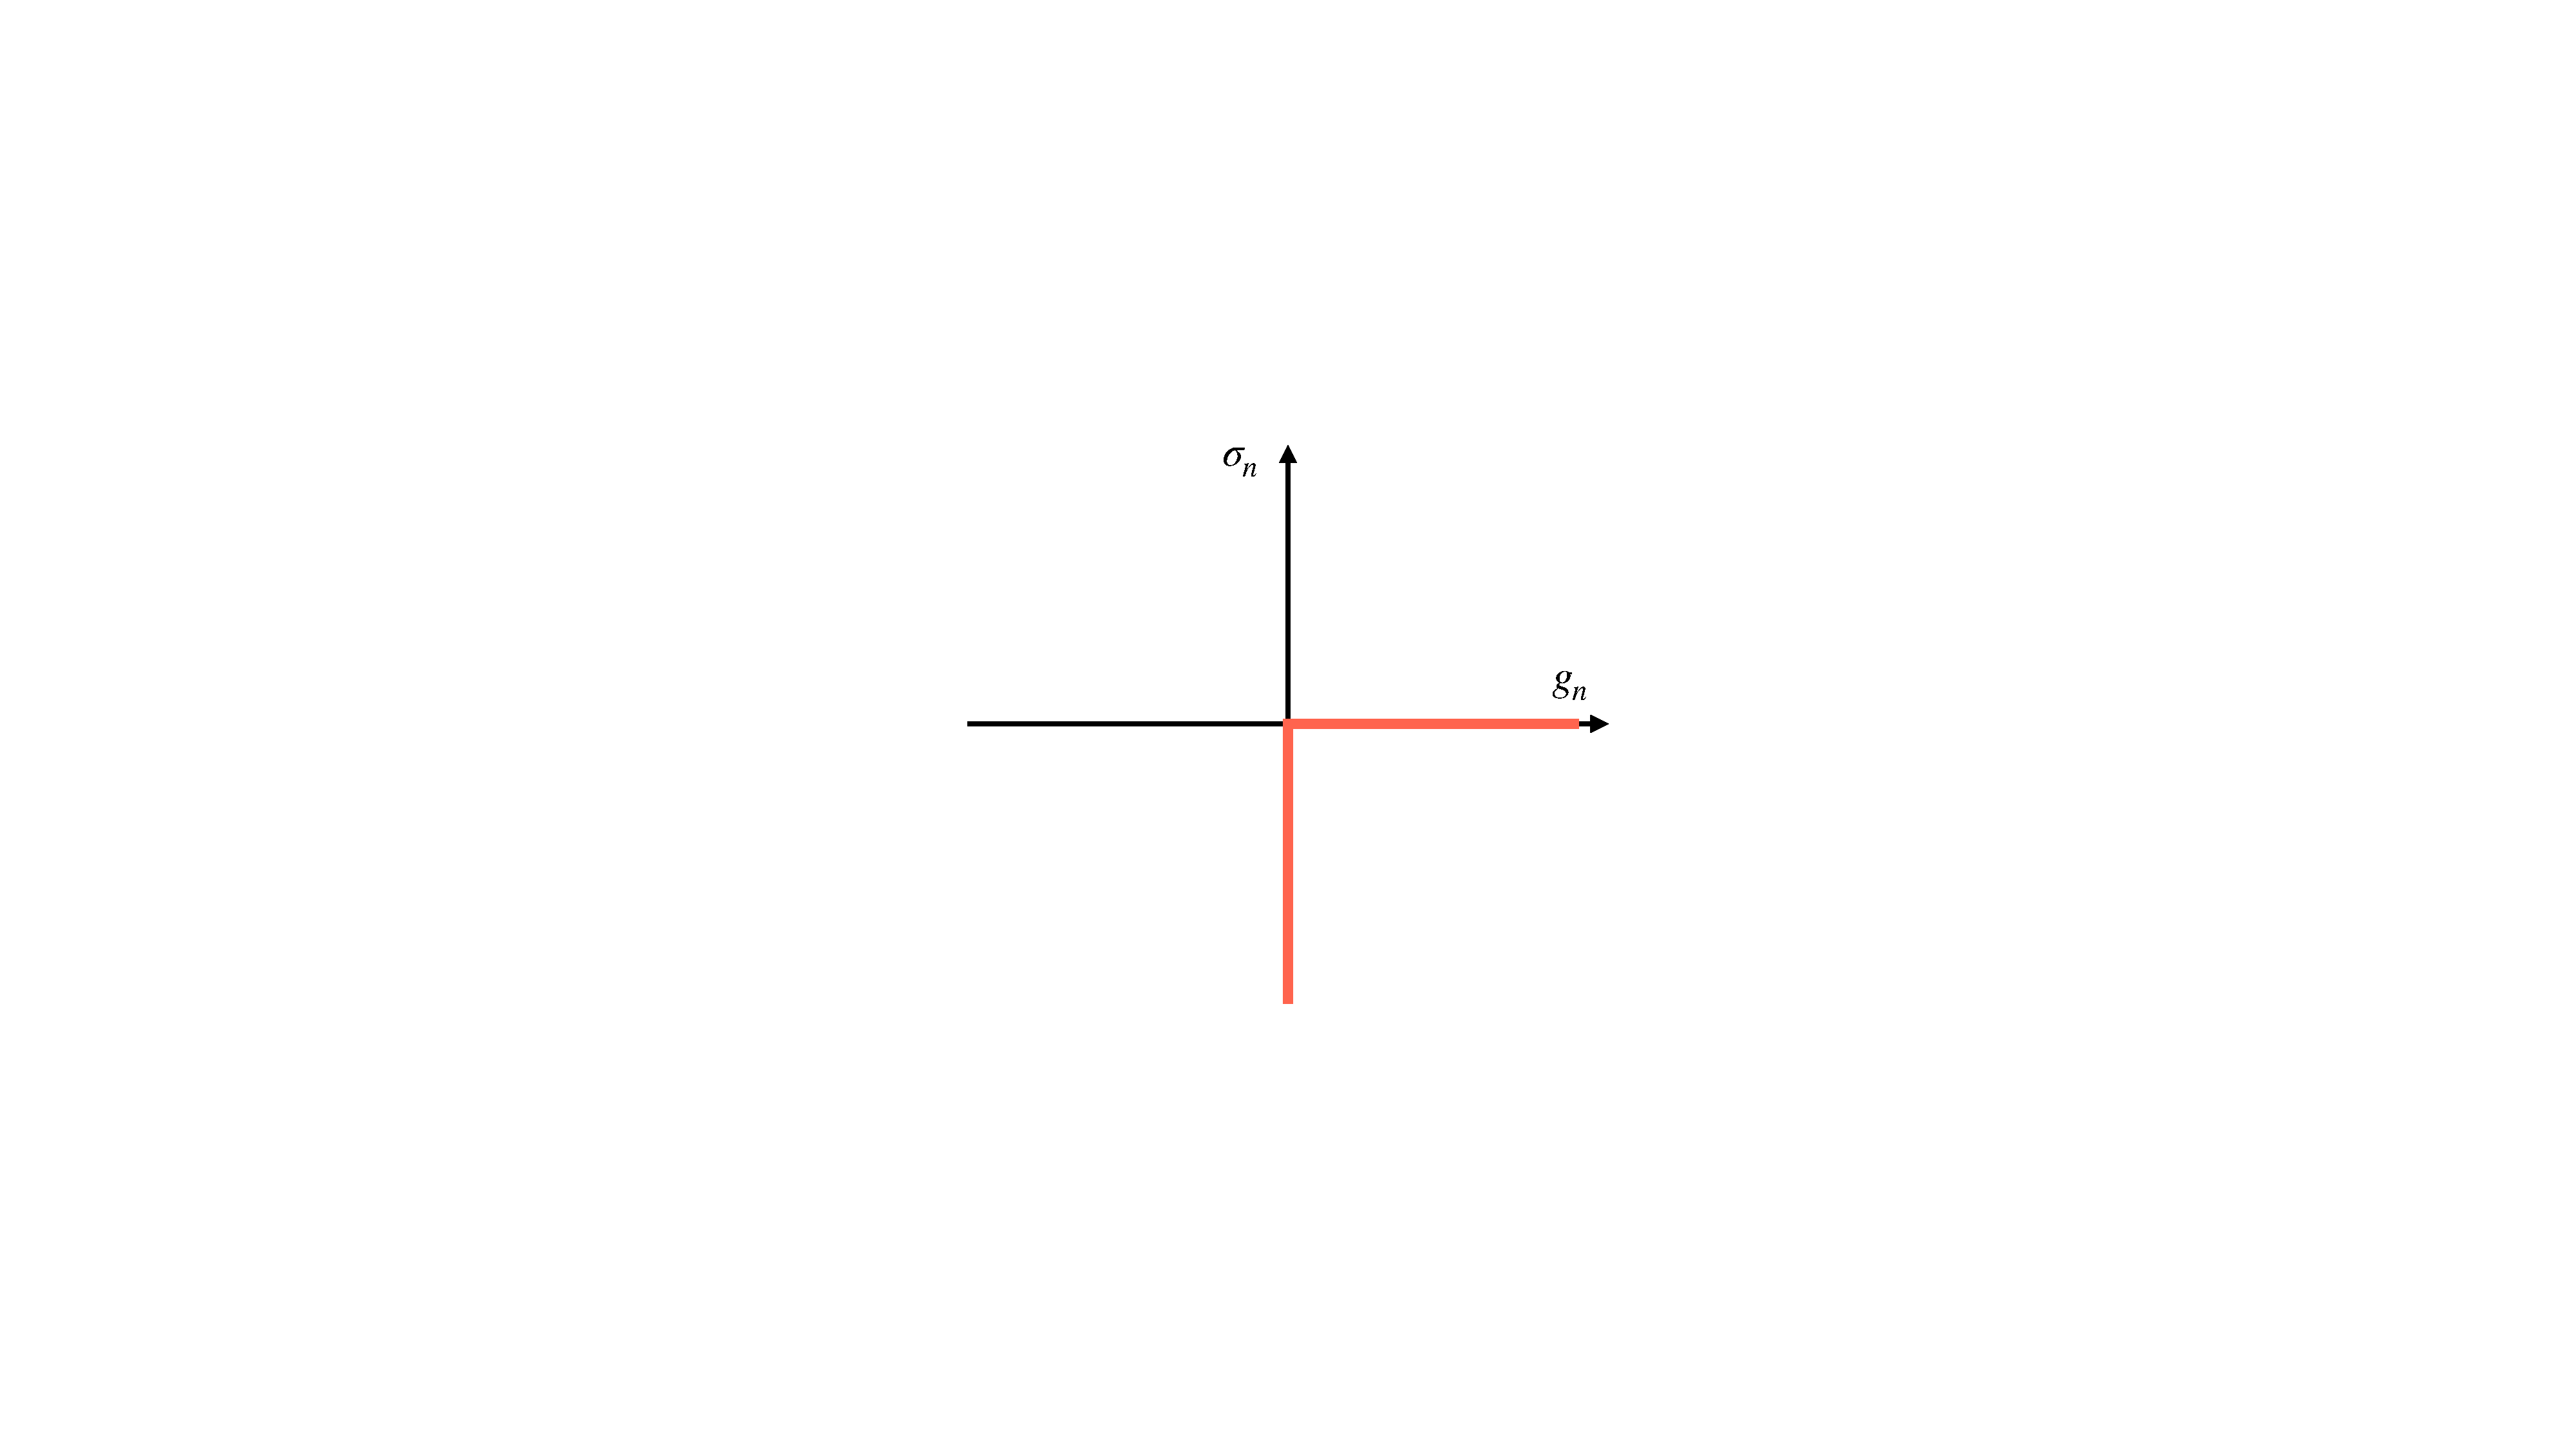
\includegraphics[scale=0.43]{Chapter1/Pictures/signorini.pdf}
    \caption{Illustration of Signorini conditions}
    \label{fig:signori}
\end{figure}

For small deformation problems, the gap function \eqref{gap_fun} can be linearised as follows

\begin{equation}\label{gap_fun}
\Delta g_n = [\bm{u}^{(1)}-\overleftarrow{\bm{u}}^{(2)}].\bm{\hat{\mathrm v}}_{n}+g_0 = u_n+g_0
\end{equation}

where $g_0$ represents the gap function in the reference configuration. Hence, for any incremental time, the linearized expression of the gap function will be used for the following definitions where the condition \eqref{no_penet} can be expressed as  

\begin{equation}
u_n+g_0 \geq 0 \quad \mathrm{or} \quad u_n-g_0 \leq 0
 \end{equation}
 
 We use the later convention  $u_n-g_0 \leq 0$ for the following definitions.


\subsection{Friction formulation}

Friction is defined through Coulomb-Amonton's law where it is based on threshold conditions to define stick and slip characteristics where no motion is allowed until $||\bm\sigma_{t}||$ satisfies the threshold $\mu ||\bm\sigma_{n}||$, defined as follows

\begin{subequations}\label{fric_bc}
\begin{equation}
|\bm{\dot{u}}_t| \geq 0
\end{equation} 

\begin{equation}
||\bm\sigma_{t}||-\mu|\sigma_{n}| \leq 0
\end{equation}

\begin{equation}
 (||\bm\sigma_{t}||-\mu|\sigma_{n}|)|\bm{\dot{u}}_t| = 0
\end{equation}

\end{subequations}

where $\mu$ is the classical coefficient of friction. The above conditions can be interpreted as follows, for the stick condition $|\bm{\dot{u}}_t|=0$,  $||\bm\sigma_{t}||\leq\mu|\sigma_{n}| $ where $||\bm\sigma_{t}||$  is inside Coulomb's cone in the space of traction stresses and similarly for the slip condition $|\bm{\dot{u}}_t|>0$,  $||\bm\sigma_{t}||=\mu|\sigma_{n}| $ where $||\bm\sigma_{t}||$ is on the Coulomb's cone. The conditions are graphically shown in Fig, \ref{fig:Coul_Amon}, similar to Signorini conditions for contact, the conditions define multi-valued mapping. \\

\begin{figure}
    \centering
    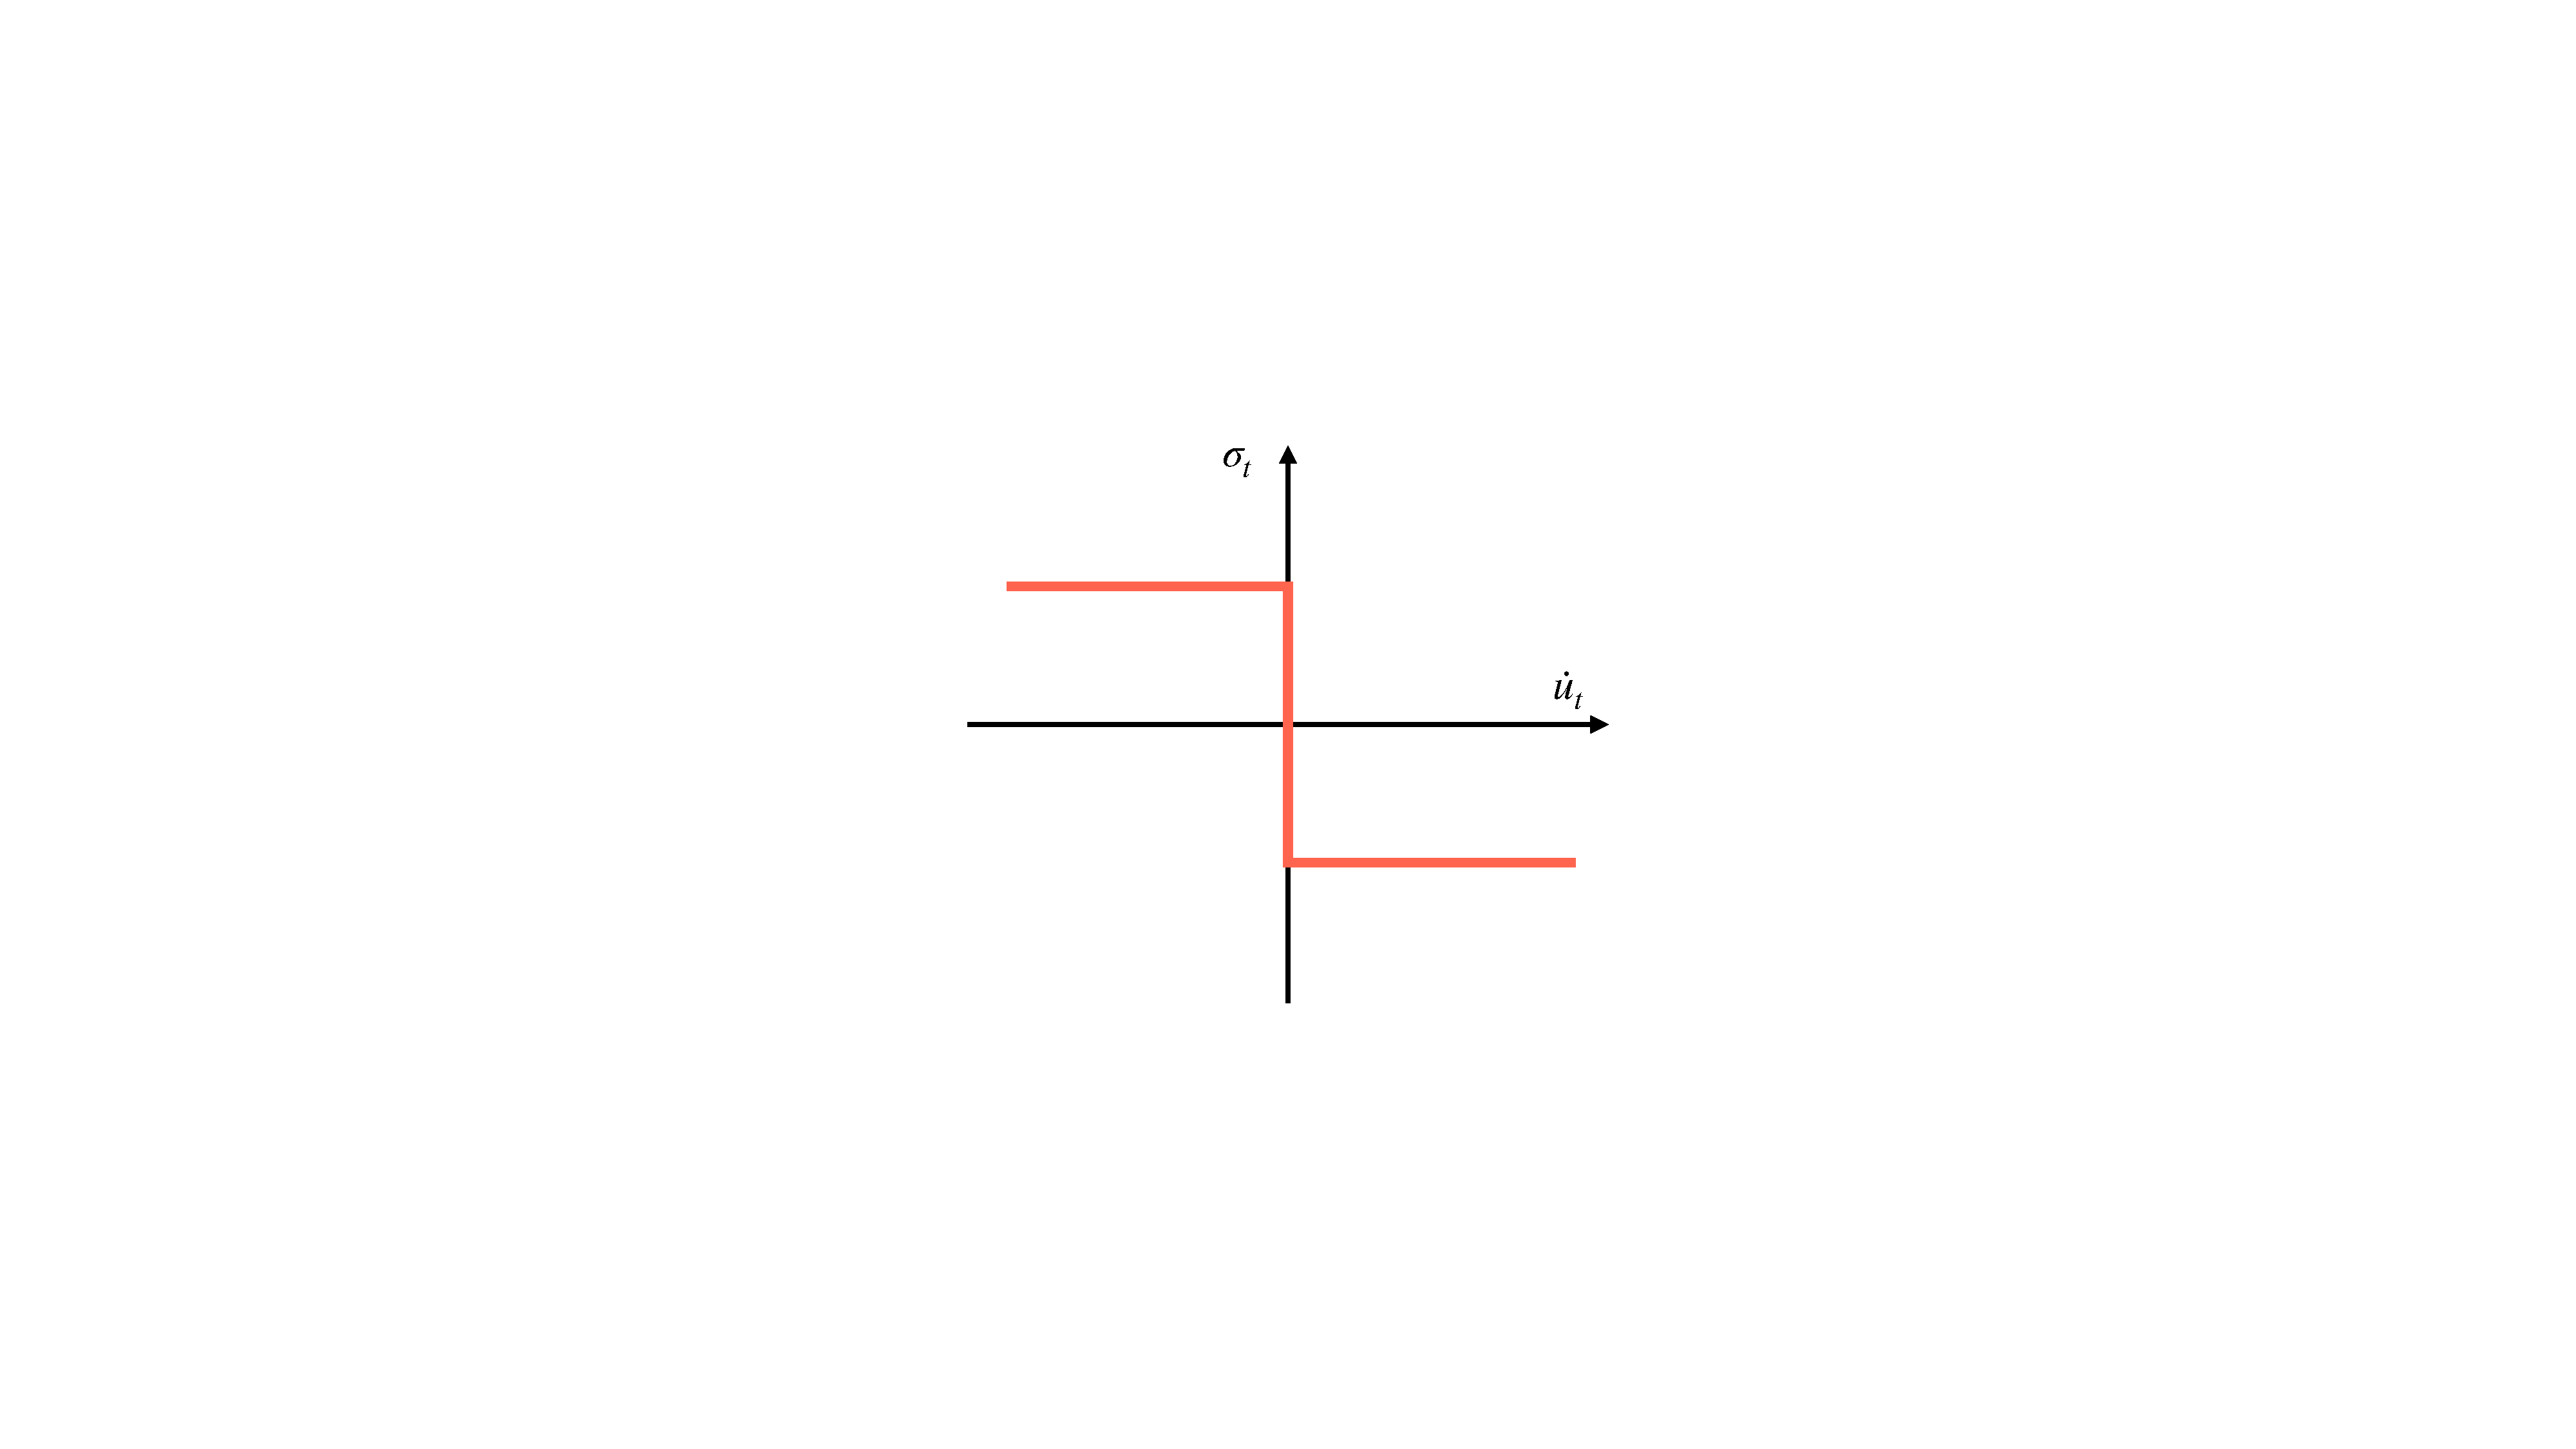
\includegraphics[scale=0.43]{Chapter1/Pictures/Coul_Amon.pdf}
    \caption{Illustration of Coulomb-Amonton's law for friction}
    \label{fig:Coul_Amon}
\end{figure}


The initial boundary value problem Eq.\eqref{cont_eq1} with unilateral conditions for contact and friction can be given as follows

\begin{equation}\label{cont_eq2}
\begin{split}
\rho\bm{\ddot{u}}+\nabla.\bm{\sigma}(\bm{u}) = \bm{f}\quad \mathrm{in} \quad \Omega\\ 
\bm{u} = \bm{u}_D\quad \mathrm{on}\quad \Gamma_D\\
\bm{\sigma}(\bm{u}).\bm{\hat{\mathrm v}}_n=\bm{t}_N\quad\mathrm{on}\quad\Gamma_N\\
%\bm{\sigma}_\mathrm{k}(u_\mathrm{k}).\hat{\mathrm v}_t=F_{f_\mathrm{k}}\quad\mathrm{on}\quad\Gamma_{c,\mathrm{k}}\\\
\\
g_n \geq 0,\quad {\sigma}_n \leq 0,\quad g_n {\sigma}_{n} = 0\quad \\
|\bm{\dot{u}}_t| = 0 \implies ||\bm\sigma_{t}||-\mu|\sigma_{n}| \leq 0\\
|\bm{\dot{u}}_t| \neq 0 \implies ||\bm\sigma_{t}||-\mu|\sigma_{n}|\frac{\bm{\dot{u}}_t}{|\bm{\dot{u}}_t|} = 0\\
\mathrm{on} \quad \Gamma_C\\
\end{split}
\end{equation}


Unlike the classical weak form \eqref{weak_f} which can be obtained through the optimisation of minimising the energy functional, the presence of inequalities from contact and friction expresses the problem in the context of convex optimisation of functional.  Hence, the weak form of the problem has the form of variational inequality where the admissible solution $\bm{\dot{u}}$ is defined over a convex set, given as follows



\begin{multline}\label{fric_con_raw}
\int_{\Omega}\rho\bm{\ddot{u}}.(\delta \bm{u}-\bm{\dot{u}}) \,\ d\Omega +\int_{\Omega}  \bm{\sigma}(\bm{u}):(\nabla \delta \bm{u}-\nabla \bm{\dot{u}}) \,\,d\Omega\\
 - \int_{\Gamma_C} \sigma_n(\delta{u}_n-{\dot{u}}_n) \,\, d\Gamma_C - \int_{\Gamma_C} \sigma_t(|\delta{\bm{u}}_t|-|{\dot{\bm{u}}}_t|) \,\, d\Gamma_C\\
  -  \int_{\Gamma_N} \bm{t}_N.(\delta \bm{u}-\bm{\dot{u}}) \,\, d\Gamma_N- \int_{\Omega} \bm{f}.(\delta \bm{u}-\bm{\dot{u}}) \,\, d\Omega \geq 0
\end{multline}


where the weak form contains the simultaneous presence of two inequalities for contact and friction. To make it complete as an initial boundary value problem, the initial conditions can be defined as $\bm{u}_0$ and $\bm{\dot{u}}_0$ which satisfies the above equation at the initial time. \\
% the function space 

The solution to the above dynamical problem is often discussed in the context of non-smooth mechanics which we do not focus here. 
%Discuss existence of sol
%The above problem characterizes rigid body motion where the solution may not be ensured. 
%The problem is often given as a quasi-static variation, where 
The existence and uniqueness of solution to the above problem  is conferred under certain conditions through regularisation of the multi-valued mapping from the Signorini conditions \eqref{cont_bc} and the Coulomb-Amonton's law \eqref{fric_bc} . Such multi-valued mapping are also seen as fundamental in defining some of the friction-induced dynamic instabilities such as stick-slip. Hence, the model for regularization and the parameters in modelling the regularization are important depending on the hypotheses that model the nature of a given instability.\\ 

We focus on modelling flutter-type dynamic instability through classical theories of linear analysis, where the effect of perturbation around a fixed point is analysed. Hence, the stability of the dynamical system with frictional contact \eqref{fric_con_raw} can be characterized by determining the fixed point which is typically quasi-static or steady-sliding equilibrium depending on the characteristics of the external forces, and defining the dynamics for the perturbation around the fixed point.
For non-linear systems such as the system with frictional contact, the stability can be defined through linearizing the perturbation around a fixed point, which brings the question of modelling the multi-valued mapping to be linear. 
This is possible through regularization of the multi-valued mapping with functions through normal-compliance approach which will be discussed in detail with the case of steady-sliding equilibrium.   
As an intermediate step in realizing the stability analysis for the steady-sliding equilibrium, we discuss the quasi-static insight for the above dynamical system \eqref{fric_con_raw}.\\


The dynamical problem can be expressed as quasi-static problem when the inertial effects can be ignored, given as 

\begin{multline}\label{fric_con_quasi}
\int_{\Omega}  \bm{\sigma}(\bm{u}):(\nabla \delta \bm{u}-\nabla \bm{\dot{u}}) \,\,d\Omega\\
 - \int_{\Gamma_C} \sigma_n(\delta{u}_n-{\dot{u}}_n) \,\, d\Gamma_C - \int_{\Gamma_C} \sigma_t(|\delta{\bm{u}}_t|-|{\dot{\bm{u}}}_t|) \,\, d\Gamma_C\\
  -  \int_{\Gamma_N} \bm{t}_N.(\delta \bm{u}-\bm{\dot{u}}) \,\, d\Gamma_N- \int_{\Omega} \bm{f}.(\delta \bm{u}-\bm{\dot{u}}) \,\, d\Omega \geq 0
\end{multline}
 
The quasi-static frictional problem characterizes the time-dependent variation of $\bm{u}_t$ with Coulomb's conditions, which implies the presence of time-dependent external forces $\bm{t}_N$ and $\bm{f}$. Hence, the system can be considered as series of quasi-static equilibrium, where the stability of the dynamical system can be characterized around such equilibrium states. 
This means that the stability could be defined taking in to account of the time-dependent external forces, or also velocity-dependent friction coefficient, where the history of loading is important for such applications. The solution to the quasi-static problem, either with uniqueness or non-uniqueness is proved to exist under strict conditions.\\

The quasi-static equilibrium can be expressed as a steady-sliding equilibrium between at least two half-spaces when no net acceleration is present. Similar to quasi-static equilibrium, this can be seen as a series of equilibrium states with respect to time where the equilibrium characteristics remain the same, except for the change in the contact domain. Since the equilibrium characteristics remain the same for all the time, the equilibrium state could be expressed with no time dependent forces but purely by static forces. This also means that the knowledge of $\bm{\hat{\mathrm v}}_t$ for ${\sigma}_t\bm{\hat{\mathrm v}}_t$ at $\Gamma_C$ is known a priori, where the general notion of  $\bm{\hat{\mathrm v}}_t$ could be given as  $\bm{\hat{\mathrm v}}_k$ for the known sliding direction. Hence, the time-independent definition of Coulomb's law could be expressed for the so-called static state as follows

\begin{subequations}
\begin{equation}
|\bm{{u}}_t| \geq 0
\end{equation} 

\begin{equation}
||\bm\sigma_{t}||-\mu|\bm\sigma_{n}| \leq 0
\end{equation}

\begin{equation}
 (||\bm\sigma_{t}||-\mu|\bm\sigma_{n}|)|\bm{{u}}_t| = 0
\end{equation}

\end{subequations}
   

The steady-sliding equilibrium explicitly defines the slip condition where the sliding velocity is constant and hence at the equilibrium, $\sigma_t = \mu\sigma_n $ at $\Gamma_C$. 
For simplicity, we consider only one half-space of the sliding contact where the half-space is considered to be fixed relative to the other half-space, while the other half-space moves parallel to $\bm{\hat{\mathrm v}}_t$ creating a sliding contact.
Hence, at any time, the equilibrium state could be expressed as follows

\begin{multline}
\int_{\Omega}  \bm{\sigma}(\bm{u}):(\nabla \delta \bm{u}-\nabla \bm{{u}}) \,\,d\Omega - \int_{\Gamma_C} \mu\sigma_n(|\delta{\bm{u}}_t|-|{{\bm{u}}}_t|) \,\, d\Gamma_C\\
  -  \int_{\Gamma_N} \bm{t}_N.(\delta \bm{u}-\bm{{u}}) \,\, d\Gamma_N- \int_{\Omega} \bm{f}.(\delta \bm{u}-\bm{{u}}) \,\, d\Omega \geq 0
\end{multline}

Since the knowledge of $\bm{\hat{\mathrm v}}_t$ for ${u}_t\bm{\hat{\mathrm v}}_t$ at $\Gamma_C$ is known a priori as $\bm{\hat{\mathrm v}}_k$ and with the slip condition for friction, the above formulation can be defined as follows

\begin{multline}\label{pre_normcomp}
\int_{\Omega}  \bm{\sigma}(\bm{u}):(\nabla \delta \bm{u}-\nabla \bm{{u}}) \,\,d\Omega - \int_{\Gamma_C} \mu\sigma_n(\delta \bm{u}-\bm{{u}}).\bm{\hat{\mathrm v}}_k \,\, d\Gamma_C\\
  -  \int_{\Gamma_N} \bm{t}_N.(\delta \bm{u}-\bm{{u}}) \,\, d\Gamma_N- \int_{\Omega} \bm{f}.(\delta \bm{u}-\bm{{u}}) \,\, d\Omega \geq 0
\end{multline}

where the multi-valued mapping of friction is replaced by a smooth definition. We now introduce the function space for defining $\delta \bm{u}$ and $\bm{{u}}$, where $\delta \bm{u}$ and $\bm{{u}}$ are defined to be from the same space $\bm K\subset \bm V $, with $\bm K$ being the convex subset of $\bm V$, given as\\

\qquad$\bm V:= \{ \delta \bm{u} \in (H^1(\Omega))^3 | \delta \bm{u}=\bm{u}_D\,\, \mathrm{on} \,\, \Gamma_D\}$\\

\qquad $\bm K:=\{\delta \bm{u} \in \bm V | \delta \bm{u}_n \leq g_n\}$\\

\qquad $\bm{f}\in (L^2(\Omega))^3$ and $\bm{t} \in (H^{-1/2}(\partial\Omega))^3$\\

where $(H^1(\Omega))^3$ is the Sobolev space of functions, given with the property\\ 

$(H^1(\Omega))^3 := \{ \delta \bm u \in (L^2(\Omega))^3, \nabla\delta \bm u  \in (L^2(\Omega))^3 \}$\\ 

Hence, the Hilbert space induced by inner product is given through $L^2$ norm:
  
${\|{\delta \bm u}\|_{L^2}= \langle {\delta \bm u},{\delta \bm u} \rangle=\int_{\Omega} {\delta \bm u}^2 d\Omega < \infty }$. A subspace $(H^{1/2}(\partial\Omega))^3$ can be defined as the restriction of $(H^{1}(\Omega))^3$ on $\partial\Omega$, where $(H^{-1/2}(\partial\Omega))^3$ is the dual of the space $(H^{1/2}(\partial\Omega))^3$.

Even though  $\bm{t}$ is typically defined to be in $L^2(\Omega)$, the unknown a priori conditions of $\bm{t}$ for $\sigma_n$ on $\Gamma_C$ results in the space to be $H^{1/2}(\partial\Omega)$.
Unlike the case for the dynamical problem or quasi-static problems which are characterized by the presence of two simultaneous inequalities, the above problem is characterized purely by the inequalities of the Signorini conditions, when friction is defined for the slip condition with equality.\\

The Signorini and Coulomb's conditions \eqref{cont_bc} \eqref{fric_bc} represent the mathematical model for contact and friction in macroscopic view, where such conditions have been found through experiments to be far from the physical reality. This leads to the view of normal compliance approach to define a better approximation of the physical reality, also through which regularization for the muti-valued mappings is achieved, where $\sigma_n$ is related as the function of gap function $g_n$ with a set of parameters determined largely by experiments, given as  

\begin{equation}\label{normal_comp}
-\sigma_n = c_n(u_n-g_n)_+^{m_n}
\end{equation}

where  $(.)_+$ allows only positive value. This can be extended to friction as follows

\begin{subequations}
\begin{equation}
|\bm{\dot{u}}_t| \geq 0
\end{equation} 

\begin{equation}
||\bm\sigma_{t}||-c_t(u_n-g_n)_+^{m_t} \leq 0
\end{equation}

\begin{equation}
 ||\bm\sigma_{t}||-c_t(u_n-g_n)_+^{m_t} |\bm{\dot{u}}_t| = 0
\end{equation}

\end{subequations}

where the parameters $c_n$, $m_n$, $c_t$ and $m_t$ are determined from the experiments. 
The normal compliance can also be applied to the previously defined dynamic and quasi-static cases, where existence and uniqueness of solution were proved through normal compliance under certain assumptions. 
For steady-sliding equilibrium, $|\bm{\dot{u}}_t|$ can be expressed as $|\bm{{u}}_t|$.\\

The Eq. \eqref{pre_normcomp} can hence be defined through normal compliance as follows

\begin{multline}
\int_{\Omega}  \bm{\sigma}(\bm{u}):(\nabla \delta \bm{u}-\nabla \bm{{u}}) \,\,d\Omega - \int_{\Gamma_C} c_t(u_n-g_n)_+^{m_t}(\delta \bm{u}-\bm{{u}}).\bm{\hat{\mathrm v}}_k \,\, d\Gamma_C\\
  -  \int_{\Gamma_N} \bm{t}_N.(\delta \bm{u}-\bm{{u}}) \,\, d\Gamma_N- \int_{\Omega} \bm{f}.(\delta \bm{u}-\bm{{u}}) \,\, d\Omega \geq 0
\end{multline}

The above variational inequality can be expressed as variational equality through active set strategy, where instead of looking for the admissible displacement field that satisfies the condition ${u}_n \leq g_n$ on $\Gamma_C$, as the minimizer of the above functional in the convex set $\bm K$ if there exists a unique solution in the set, the set $\Gamma_C$ is defined a priori, called active set, at least for an incremental time for which ${u}_n  - g_n \rightarrow 0$, provided that ${u}_n \leq g_n$ was satisfied prior to the given time. 
With the knowledge of active set, the displacement field $u_n$ on $\Gamma_C$ could be satisfied by normal compliance given in Eq. \eqref{normal_comp}.
Hence, the above functional with inequality can be expressed through equality as follows

 \begin{multline}\label{SS_pen}
\int_{\Omega}  \bm{\sigma}(\bm{u}):\nabla \delta \bm{u} \,\,d\Omega - 
\underbrace{\int_{\Gamma_C} c_t(u_n-g_n)_+^{m_t}\delta \bm{u}.\bm{\hat{\mathrm v}}_k \,\, d\Gamma_C}_{{\langle \bm{\sigma}_n, \delta \bm u \rangle}} 
+ \underbrace{\int_{\Gamma_C} c_n(u_n-g_n)_+^{m_n}\delta \bm{u}.\bm{\hat{\mathrm v}}_n \,\, d\Gamma_C}_{{\langle \bm{\sigma}_t, \delta \bm u \rangle}}\\
  -  \int_{\Gamma_N} \bm{t}_N.\delta \bm{u} \,\, d\Gamma_N- \int_{\Omega} \bm{f}.\delta \bm{u} \,\, d\Omega = 0
\end{multline}

where the inner products ${\langle \bm{\sigma}_n, \delta \bm u \rangle}$ and ${\langle \bm{\sigma}_t, \delta \bm u \rangle}$ define the  weak form of contact and friction respectively. 
The definition of $\Gamma_C$ through the active set strategy means that $\bm{t}_N \in (L^2(\Omega))^3$. 
 When $m_n \neq 1$ and $m_t \neq 1$, the steady-sliding equilibrium can be solved through non-linear programming like Newton-Rhapson for $\bm{u}_{eq}$.\\ 
 
We do not relate to the experimental determination of the parameters $c_n$, $m_n$, $c_t$ and $m_t$. Hence, $c_n$ is purely given as the penalty parameter $\mathit{p}$ considering numerical stability, which implies that for any $(u_n-g_0) > 0$ defined by $(u_n-g_0)_+$ is penalized by a factor $p$, where the ideal would be $ \mathit{p} \rightarrow \infty$. 
While $c_t$ is given for the ideal slip state of the steady-sliding equilibrium as $c_t=\mu\mathit{p}$. 
The normal compliance approach can be viewed in general as modelling springs with certain stiffness $c_n$ which resist penetration at the contact interface. 
We consider $m_n = m_t = 1$, where the parameters $m_n$ and $m_t$ for any value other than $1$ can be physically interpreted as non-linear springs. 
With the above consideration of the parameters for the normal compliance, the above functional can be expressed as follows

 \begin{multline}\label{SS_pen_1}
\int_{\Omega}  \bm{\sigma}(\bm{u}):\nabla \delta \bm{u} \,\,d\Omega - \int_{\Gamma_C} \mu\mathit{p}(u_n-g_n)_+\delta \bm{u}.\bm{\hat{\mathrm v}}_k \,\, d\Gamma_C + \int_{\Gamma_C} \mathit{p}(u_n-g_n)_+\delta \bm{u}.\bm{\hat{\mathrm v}}_n \,\, d\Gamma_C\\
  -  \int_{\Gamma_N} \bm{t}_N.\delta \bm{u} \,\, d\Gamma_N- \int_{\Omega} \bm{f}.\delta \bm{u} \,\, d\Omega = 0
\end{multline}




where for finite deformation, the problem can be solved for $\bm{u}_{eq}$ with one incremental time step.\\

The perturbed state of the displacement field for any excitation of the steady-sliding equilibrium can be given as 

\begin{equation}\label{pert_wrt_eq}
\bm{u}=\bm{u}_{eq}+\bm{\widetilde{u}}
\end{equation}

 where $\bm{\widetilde{u}}$ corresponds to the perturbed displacement field. The idea is to analyse the dynamics of the perturbation such that the stability of the dynamical system can be determined through the onset evolution of the dynamics for the perturbation, where it is hypothesized that the onset evolution of the dynamics can be expressed linearly. This brings the question of linearization for the non-linear frictional contact problem, even with the sufficient approximation made for Eq. \eqref{SS_pen_1}.\\

 As a detour for generalization, we discuss the linearization of the normal compliance terms. The contact and friction terms in Eq. \eqref{SS_pen} with $c_n=p, c_t=\mu p$, $0< m_n \neq 1$  and $0< m_t \neq 1$ , can be expressed as\\ 
 
 \begin{subequations}\label{genli}
 \begin{equation}
 {\langle \bm{\sigma}_n, \delta \bm u \rangle_{\Gamma_C}}=\int_{\Gamma_C} \mathit{p}(u_n-g_0)^{m_n}_+\delta \bm{u}.\bm{\hat{\mathrm v}}_n \,\, d\Gamma_C
  \end{equation}
  \begin{equation}
  {\langle \bm{\sigma}_t, \delta \bm u \rangle_{\Gamma_C}}= \int_{\Gamma_C} \mu\mathit{p}(u_n-g_0)^{m_t}_+\delta \bm{u}.\bm{\hat{\mathrm v}}_k \,\, d\Gamma_C
  \end{equation}
 \end{subequations}
 
 
% when $m_n \neq 1$ and $m_t \neq 1$, the steady-sliding equilibrium can be solved through non-linear programming like Newton-Rhapson for $\bm{u}_{eq}$.\\ 
 
 The perturbation of the normal compliance can hence be expressed as\\
 
  \begin{subequations}
 \begin{equation}
 \mathit{p}(\widetilde{u}_n+u_n-g_n)^{m_n}_+- \mathit{p}(u_n-g_0)^{m_n}_+\approx \mathit{p}(\widetilde{u}_n)^{m_n}_+
   \end{equation}
    \begin{equation}
 \mu\mathit{p}(\widetilde{u}_n+u_n-g_n)^{m_t}_+- \mu\mathit{p}(u_n-g_0)^{m_t}_+\approx \mu\mathit{p}(\widetilde{u}_n)^{m_t}_+
    \end{equation}
  \end{subequations}
  
 if it can be assumed that the parameters of the normal compliance stay the same for the perturbation $\bm{\widetilde{u}}$ close to the equilibrium $\bm{u}_{eq}$. The linearization for the degree of the polynomial terms at $\bm{u}_{eq}$ can be defined as\\
 
 \begin{subequations}
 \begin{equation}
  \Delta \mathit{p}(\widetilde{u}_n)^{m_n}_+ |_{\bm{u}_{eq}}
 = m_n \mathit{p}(\widetilde{u}_n)^{m_n-1}_+|_{\bm{u}_{eq}}
 \end{equation}
  \begin{equation}
   \Delta \mu\mathit{p}(\widetilde{u}_n)^{m_t}_+ |_{\bm{u}_{eq}}
   = \mu m_t \mathit{p}(\widetilde{u}_n)^{m_t-1}_+|_{\bm{u}_{eq}}
  \end{equation}
 \end{subequations}
 
where the expressions are still non-linear in the presence of $(.)_+$. It should be noted that the perturbation $\widetilde{u}_n$ on $\Gamma_C$ may not result in the same active set as the equilibrium, due to the possible separation at some parts on $\Gamma_C$, which introduces non-linearities defined by $(.)_+$. 
 This is because the separation leads to $u_n-g_0 < 0$ and hence $p(u_n-g_0)_+^{m_n} \rightarrow 0$ which can only be taken in to account nonlinearly. 
 This is linearized with the hypothesis that the onset of instability occurs very close to the equilibrium $\bm{u}_{eq}$ such that $\Gamma_C$ remains the same for the perturbation $\bm{\widetilde{u}}$. This means that if $\Gamma_C$ must be constant for $\widetilde{\bm{u}}$, the separation $u_n-g_0 < 0$ must also be penalized which can simply be achieved by evading the operator $(.)_+$ .  
The above hypothesis for the perturbation of $\widetilde{u}_n$ on $\Gamma_C$ would have been impossible to define with Signorini conditions where $\widetilde{u}_n$ may lead to strict contact separation on $\Gamma_C$, while in the view of normal compliance, the perturbation $\widetilde{u}_n$ for no variation of $\Gamma_C$ can be considered to  define the variation of $\sigma_n$ and hence also its subsequent effect on $\sigma_t$ for friction.\\
  
With the above hypothesis, the linearized weak form of contact and friction for the dynamics of the perturbation $\bm{\widetilde{u}}$ close to $\bm{u}_{eq}$ can be defined as\\
 
 \begin{subequations}
 \begin{equation}
 {\langle \bm{\sigma}_n, \delta \bm u \rangle_{\Gamma_C}}= \int_{\Gamma_C} m_n\mathit{p}{\widetilde{u}_n}^{\,m_n-1}|_{\bm{u}_{eq}}\delta \bm{u}.\bm{\hat{\mathrm v}}_n \,\, 
 d\Gamma_C
 \end{equation}
 \begin{equation}
  {\langle \bm{\sigma}_t, \delta \bm u \rangle_{\Gamma_C}}=\int_{\Gamma_C} \mu m_n\mathit{p}{\widetilde{u}_n}^{\,m_n-1}|_{\bm{u}_{eq}}\delta \bm{u}.\bm{\hat{\mathrm v}}_k \,\, d\Gamma_C\\
 \end{equation}
 \end{subequations}
 %This can be assumed that the $c_n = p$ and $c_n = p$ is purely determined 
It should be noted that the above weak form is different from the classical weak form of contact and friction defined by normal compliance in Eq. \eqref{SS_pen}. The above weak form essentially characterises force which is purely displacement-dependent, also known as follower force. The definition of follower force can be largely said as implicit for modelling flutter-type dynamic instability. 
In the case of flutter-type instability arising from friction between solids, the main hypothesis is that the onset of instability occurs at perturbations very close to $\bm u_{eq}$ such that the non-linearities of the classical contact and friction \eqref{SS_pen} can be effectively ignored and hence, friction phenomenon for a perturbed state $\widetilde{\bm u}$ can be modelled linearly with the contact state of $\bm u_{eq}$ purely by displacement-dependent forces.
Hence, the hypothesis only characterises $\widetilde{\bm u}$ with the linearization of non-linearities very close to $\bm u_{eq}$, while the characteristics of non-linearities away from $\bm u_{eq}$ cannot be forseen.
This essentially reflects on the possibility of utilising linear analysis such as CEA \ref{Phy_CEA}, where CEA can characterise instability of a system through eigenmodes in one computation, which would otherwise require expensive transient analysis to find a limit cycle.
This defines the system to be holonomic and autonomous since the nature of follower force depends only on generalized coordinates without explicit time dependence. 
%It should be noted that linearization effectively models instabilities very close to the equilibrium, while the effect of non-linearities away from $\bm u_{eq}$ is not present. \\

We consider the case of $m_n = 1$ and $m_t = 1$ for the following discussions, where the linearization of Eqs. \eqref{genli} can simply be expressed as\\ 
 
 \begin{subequations}
 \begin{equation}
 {\langle \bm{\sigma}_n, \delta \bm u \rangle_{\Gamma_C}}= \int_{\Gamma_C} \mathit{p}{\widetilde{u}_n}\delta \bm{u}.\bm{\hat{\mathrm v}}_n \,\, d\Gamma_C
   \end{equation}
   \begin{equation}
  {\langle \bm{\sigma}_t, \delta \bm u \rangle_{\Gamma_C}}= \int_{\Gamma_C} \mu \mathit{p}{\widetilde{u}_n}\delta \bm{u}.\bm{\hat{\mathrm v}}_k \,\, d\Gamma_C
     \end{equation}
   \end{subequations}
   
 The initial-boundary value problem for the dynamics of the perturbation can be given as
 
\begin{equation}\label{pert_dyn}
\begin{split}
\rho^\mathrm{(k)}\bm{\ddot{\widetilde{u}}}^\mathrm{(k)} +\nabla\bm{.}\bm{\sigma}^\mathrm{(k)}(\bm{\widetilde u}^\mathrm{(k)}) = 0 \quad \mathrm{in} \quad \Omega^\mathrm{(k)}\\ 
\bm{\widetilde u}^\mathrm{(k)} = \bm{\widetilde u}^\mathrm{(k)}_{D} \quad \mathrm{on}\quad\Gamma^{\mathrm{(k)}}_D\\
\sigma^{(\mathrm k)}_n(\bm{\widetilde u}^\mathrm{(k)}) \bm{\hat{\mathrm v}}_n = - \mathit{p}{\widetilde{u}_n}^{(\mathrm k)} \bm{\hat{\mathrm v}}_n,\quad \sigma^{(\mathrm k)}_t(\bm{\widetilde u}^\mathrm{(k)})  \bm{\hat{\mathrm v}}_k = \mu \mathit{p}{\widetilde{u}_n}^{(\mathrm k)} \bm{\hat{\mathrm v}}_k \quad \mathrm{on}\quad\Gamma^{\mathrm{(k)}}_C\\
%\bm{\sigma}_\mathrm{k}(u_\mathrm{k}).\hat{\mathrm v}_t=F_{f_\mathrm{k}}\quad\mathrm{on}\quad\Gamma_{c,\mathrm{k}}\\
\end{split}
\end{equation}

It should be noted that for linear case, the problem can be explicitly defined without the fore knowledge of $\bm u_{eq}$, by defining $\Gamma_C$ explicitly. For simplicity, we consider the parameters $p$ and $\mu$ to be constant between the contact interface of all the domains in contact. The subscript $\mathrm{k}$ distinguishes the domains in contact.  Similar to Eq. \eqref{weak_f}, the weak form of the differential formulation can be expressed as

\begin{equation} \label{weak_pert}
\int_{\Omega^{(k)}}\rho^\mathrm{(k)}\bm{\ddot{\widetilde{u}}}^\mathrm{(k)}. \delta\bm u^\mathrm{(k)} \,\,d\Omega^\mathrm{(k)} +\int_{\Omega^{(k)}} \bm{\sigma}^\mathrm{(k)}(\bm{\widetilde u}^\mathrm{(k)}) : \nabla\delta\bm u^\mathrm{(k)} \,\,d\Omega^\mathrm{(k)} - \int_{\Gamma^{(k)}_C} \bm t_C^\mathrm{(k)}  .  \delta\bm u^\mathrm{(k)} \,\,d\Gamma_{C}^\mathrm{(k)} = 0 
\end{equation}
 
The traction force $\bm t_C \in H^{-{1}/{2}}(\Gamma_C)$ can be decomposed as follows

\begin{equation}
\begin{split}
 \int_{\Gamma^{(\mathrm k)}_C}  \bm t_C^\mathrm{(k)}  .  \delta\bm u^\mathrm{(\mathrm k)}  \,\,d\Gamma_{C}^\mathrm{(k)} = \int_{\Gamma^{(k)}_C} ( \sigma_n^{(\mathrm k)} \bm{\hat{\mathrm v}}_n+  \sigma_t^{(\mathrm k)}\bm{\hat{\mathrm v}}_k) .
 \delta\bm u^\mathrm{(k)} \,\,d\Gamma_{C}^\mathrm{(k)}\\ 
 =  {\int_{\Gamma^{(k)}_C}  \sigma_n^{(\mathrm k)} \bm{\hat{\mathrm v}}_n. \delta\bm u^\mathrm{(k)}} \,\,d\Gamma_{C}^\mathrm{(k)}+ {\int_{\Gamma^{(k)}_C}  \sigma_t^{(\mathrm k)} \bm{\hat{\mathrm v}}_k. \delta\bm u^\mathrm{(k)}} \,\,d\Gamma_{C}^\mathrm{(k)}
 \end{split}
\end{equation}

Hence, the Eq. \eqref{weak_pert} for the $\mathrm n_{\mathrm k}$ domains in contact can be defined as 

\begin{multline} 
\sum_{\mathrm{k}=1}^{\mathrm{n}_{\mathrm{\mathrm{k}}}}   \bigg\{  \int_{\Omega^{(k)}}\rho^\mathrm{(k)}\bm{\ddot{\widetilde{u}}}^\mathrm{(k)}. \delta\bm u^\mathrm{(k)} \,\,d\Omega^\mathrm{(k)}+\int_{\Omega^{(k)}} \bm{\sigma}^\mathrm{(k)}(\bm{\widetilde u}^\mathrm{(k)}) : \nabla \delta\bm u^\mathrm{(k)} \,\,d\Omega^\mathrm{(k)}\\  -    \underbrace{\int_{\Gamma^{(k)}_C}  \sigma_n^{(\mathrm k)} \bm{\hat{\mathrm v}}_n. \delta\bm u^\mathrm{(k)}  \,\,d\Gamma_{C}^\mathrm{(k)}}_{\langle \bm{\sigma}^{\mathrm{(k)}}_n, \delta \bm u^{\mathrm{(k)}} \rangle_{\Gamma_C^{\mathrm{(k)}}}} - \underbrace{\int_{\Gamma^{(k)}_C}  \sigma_t^{(\mathrm k)} \bm{\hat{\mathrm v}}_k. \delta\bm u^\mathrm{(k)}  \,\,d\Gamma_{C}^\mathrm{(k)}}_{\langle \bm{\sigma}^{\mathrm{(k)}}_t, \delta \bm u^{\mathrm{(k)}} \rangle_{\Gamma_C^{\mathrm{(k)}}}} \bigg\} = 0 
\end{multline}\label{weak_pert_1}

where $\bm \sigma_n, \bm \sigma_t \in (H^{-1/2}(\Gamma_C))^3$.  The inner products can be expressed in $(H^{1/2}(\Gamma_C))^{3}$ space which is the restriction of $\bm u \in H^{1}(\Omega) \rightarrow H^{1/2} (\Gamma_C)$  through the normal compliance approach, where the above equation can be defined as  

\begin{multline}  
\sum_{\mathrm{k}=1}^{\mathrm{n}_{\mathrm{\mathrm{k}}}}   \bigg\{  \int_{\Omega^{(k)}}\rho^\mathrm{(k)}\bm{\ddot{\widetilde{u}}}^\mathrm{(k)}. \delta\bm u^\mathrm{(k)} \,\,d\Omega^\mathrm{(k)}+\int_{\Omega^{(k)}} \bm{\sigma}^\mathrm{(k)}(\bm{\widetilde u}^\mathrm{(k)}) : \nabla \delta\bm u^\mathrm{(k)} \,\,d\Omega^\mathrm{(k)}\\  
+ \underbrace{\int_{\Gamma^{(k)}_C}  \mathit{p}{\widetilde{u}_n}^{(\mathrm k)} \bm{\hat{\mathrm v}}_n. \delta\bm u^\mathrm{(k)}  \,\,d\Gamma_{C}^\mathrm{(k)}}_{\langle \bm{\sigma}^{\mathrm{(k)}}_n, \delta \bm u^{\mathrm{(k)}} \rangle_{\Gamma_C^{\mathrm{(k)}}}} 
- \underbrace{\int_{\Gamma^{(k)}_C} \mu \mathit{p}{\widetilde{u}_n}^{(\mathrm k)} \bm{\hat{\mathrm v}}_k. \delta\bm u^\mathrm{(k)}  \,\,d\Gamma_{C}^\mathrm{(k)}}_{\langle \bm{\sigma}^{\mathrm{(k)}}_t, \delta \bm u^{\mathrm{(k)}} \rangle_{\Gamma_C^{\mathrm{(k)}}}} \bigg\} = 0 
\end{multline}

For simplicity in expansion of the contact and friction compliance terms, we consider contact between two domains $\Omega^{(a)}$ and $\Omega^{(b)}$, with the derivation of traction forces on $\Omega^{(a)}$. Hence, the inner products ${\langle \bm{\sigma}^{\mathrm{(a)}}_n, \delta \bm u^{\mathrm{(a)}} \rangle_{\Gamma_C^{\mathrm{(a)}}}}$ and ${\langle \bm{\sigma}^{\mathrm{(a)}}_t, \delta \bm u^{\mathrm{(a)}} \rangle_{\Gamma_C^{\mathrm{(a)}}}}$ can be expressed as
 
\begin{equation}\label{pert_cont}
{\langle \bm{\sigma}^{\mathrm{(a)}}_n, \delta \bm u^{\mathrm{(a)}} \rangle_{\Gamma_C^{\mathrm{(a)}}}} = 
\int_{\Gamma^{(\mathrm a)}_C}  \mathit{p}{\widetilde{u}_n}^{(\mathrm a)} \bm{\hat{\mathrm v}}_n. \delta\bm u^\mathrm{(a)} \,\,d\Gamma_{C}^\mathrm{(a)}=
\int_{\Gamma^{(\mathrm a)}_C}  \mathit{p}[({\widetilde{\bm u}}^{(\mathrm a)} - {\widetilde{\bm u}}^{(\mathrm b)}). \bm{\hat{\mathrm v}}_n]  \delta\bm u^\mathrm{(a)}. \bm{\hat{\mathrm v}}_n \,\,d\Gamma_{C}^\mathrm{(a)}
\end{equation}

\begin{equation}\label{pert_fric}
{\langle \bm{\sigma}^{\mathrm{(a)}}_t, \delta \bm u^{\mathrm{(a)}} \rangle_{\Gamma_C^{\mathrm{(a)}}}} = 
\int_{\Gamma^{(\mathrm a)}_C}  \mu \mathit{p}{\widetilde{u}_n}^{(\mathrm a)} \bm{\hat{\mathrm v}}_n. \delta\bm u^\mathrm{(a)} \,\,d\Gamma_{C}^\mathrm{(a)}=
\int_{\Gamma^{(\mathrm a)}_C}  \mu \mathit{p}[({\widetilde{\bm u}}^{(\mathrm a)} - {\widetilde{\bm u}}^{(\mathrm b)}). \bm{\hat{\mathrm v}}_n] \delta\bm u^\mathrm{(a)}. \bm{\hat{\mathrm v}}_k \,\,d\Gamma_{C}^\mathrm{(a)}
\end{equation}

The traction forces on $\Omega^{(b)}$ can similarly be defined from the conservation of momentum as $\bm{\sigma}^{\mathrm{(a)}}_n = - \bm{\sigma}^{\mathrm{(b)}}_n$ and $\bm{\sigma}^{\mathrm{(a)}}_t = - \bm{\sigma}^{\mathrm{(b)}}_t$. 
We defined a suitable function space $\bm V \subset (H^1(\Omega))^3$ on which the solution $\bm u$ of the functional in modelling the continuum is presumed to exist.The arbitrary variation $\delta \bm u$ in an infinite-dimensional function space $\bm V$ can be expressed as

\begin{equation}
\delta \bm u = \sum^{\infty}_\mathrm{i}  \delta \bm \vartheta_\mathrm{i} \bm v_i \qquad \forall  \bm v_i \in \bm V
\end{equation}

Hence, the Eq. \eqref{weak_pert_1} can be defined for a system of two domains $\Omega^{(a)}$ and $\Omega^{(b)}$as 


\begin{multline} \label{weak_pert_2}
\sum^{\mathrm{a,b}}_{\mathrm{k}}    \bigg\{   \bigg( \int_{\Omega^{(k)}}\rho^\mathrm{(k)}\bm{\ddot{\widetilde{u}}}^\mathrm{(k)}.  \bm v_i^\mathrm{(k)} \,\,d \Omega^{(k)}+\int_{\Omega^{(k)}} \bm{\sigma}^\mathrm{(k)}(\bm{\widetilde u}^\mathrm{(k)}) : \nabla \bm v_i^\mathrm{(k)}\,\,d \Omega^{(\mathrm k)}\\  
+\int_{\Gamma^{(k)}_C}  \mathit{p}[({\widetilde{\bm u}}^{(\mathrm k)} - {\widetilde{\bm u}}^{( \sim \mathrm k)}). \bm{\hat{\mathrm v}}_n]  \bm v_i^\mathrm{(k)}. \bm{\hat{\mathrm v}}_n \,\,d{\Gamma^{(k)}_C} 
-\int_{\Gamma^{(k)}_C}  \mu \mathit{p}[({\widetilde{\bm u}}^{(\mathrm k)} - {\widetilde{\bm u}}^{(\sim \mathrm k)}). \bm{\hat{\mathrm v}}_n]  \bm v_i^\mathrm{(k)}. \bm{\hat{\mathrm v}}_k \,\,d{\Gamma^{(\mathrm k)}_C} \bigg) \delta \bm \vartheta  \bigg\} = 0 
\end{multline} 

where the equation must be satisfied for any arbitrary variation of $\delta \bm \vartheta$. $\sim \mathrm k$ defines the domain which is not $\mathrm k$, i.e., $\mathrm{k=a}$ implies $\sim\mathrm{k=b}$ and vice-versa.\\

With the finite element approach, we define a finite-dimensional function space ${}_h \bm {V} \subset \bm V$ and hence, there is some bound for ${}_h \bm v_\mathrm{i} \in {}_h \bm V$. We define the approximation of $\bm u$ in the same space ${}_h \bm V$ as $\bm u \approx {}_h \bm u \in {}_h \bm V$, where the above equation can be defined as

\begin{multline} \label{weak_pert_2}
\sum^{\mathrm{a,b}}_{\mathrm{k}}   \bigg\{ \int_{\Omega^{(k)}}\rho^\mathrm{(k)} {}_h\bm{\ddot{\widetilde{u}}}^\mathrm{(k)}. {}_h \bm v_i^\mathrm{(k)}  \,\,d \Omega^{(\mathrm k)} +\int_{\Omega^{(k)}} \bm{\sigma}^\mathrm{(k)}({}_h \bm{\widetilde u}^\mathrm{(k)}) : \nabla {}_h \bm v_i^\mathrm{(k)} \,\,d \Omega^{(\mathrm k)}\\  
+\int_{\Gamma^{(k)}_C}  \mathit{p}[({{}_h\widetilde{\bm u}}^{(\mathrm k)} - {{}_h \widetilde{\bm u}}^{ (\sim \mathrm k)}). \bm{\hat{\mathrm v}}_n]  {}_h \bm v_i^\mathrm{(k)}. \bm{\hat{\mathrm v}}_n \,\,d{\Gamma^{(\mathrm k)}_C}
-\int_{\Gamma^{(k)}_C}  \mu \mathit{p}[({{}_h\widetilde{\bm u}}^{(\mathrm k)} - {{}_h\widetilde{\bm u}}^{(\sim \mathrm k)}). \bm{\hat{\mathrm v}}_n]  {}_h \bm v_i^\mathrm{(k)}. \bm{\hat{\mathrm v}}_k \,\,d{\Gamma^{(\mathrm k)}_C} \bigg\} = 0 \\
\qquad \forall {}_h \bm v_i^{(\mathrm k)} \in {}_h \bm V^{(\mathrm k)}
\end{multline} 

We explain the definition of space ${}_h \bm V$ for classical finite elements in ~, but we mainly explain in detail for Isogeometric methods with focus on contact in ~, where the Isogeometric approach is new for the given application. 
But given a suitable choice of finite-dimensional space ${}_h \bm V$, the above equation can be defined in matrix form as  

\begin{equation}\label{mat_dyn_fric}
\mathbf M^{(a-b)} \ddot{\bm{\widetilde U}}^{(a-b)} +(\mathbf K^{(a-b)} +\mathbf K_C^{(a-b)}+\mathbf K_F^{(a-b)}) \bm{\widetilde{U}}^{(a-b)} =0
\end{equation}

The properties of the matrices can be given as follows, where $\mathbf M$ and $\mathbf K$ are symmetric and positive definite. $\mathbf K_C$ is also symmetric which essentially defines the conservation of momentum at the interface, while $\mathbf K_F$ is non-symmetric with the non-conservative nature of friction at slip state. 
Often damping matrix $\mathbf C$ is also added purely in numerical context, typically through modal or Rayleigh damping. In the scope of modelling rotational inertia effects, gyroscopic matrix $\mathbf G$ can also be defined, where $\mathbf {C}$ and  $\mathbf {G}$ are both velocity dependent. We do not consider damping and gyroscopic effects for the following discussions, where we mainly focus on contact and friction definitions.\\

With the definition of finite-dimensional space ${}_h \bm V$, the steady-sliding problem can be expressed as

 \begin{multline}
 \sum^{\mathrm{a,b}}_{\mathrm{k}}   \bigg\{ \int_{\Omega}  \bm{\sigma}^\mathrm{(k)}({}_h\bm{u}^\mathrm{(k)}):\nabla {}_h \bm v_i^\mathrm{(k)} \,\,d\Omega - \int_{\Gamma_C} \mu\mathit{p}({}_hu_n^\mathrm{(k)}-{}_hg_n)_+\,{}_h \bm v_i^\mathrm{(k)}.\bm{\hat{\mathrm v}}_k \,\, d\Gamma_C\\ + \int_{\Gamma_C} \mathit{p}({}_hu_n^\mathrm{(k)}-{}_hg_n)_+\,{}_h \bm v_i^\mathrm{(k)}.\bm{\hat{\mathrm v}}_n \,\, d\Gamma_C
  -  \int_{\Gamma_N} {}_h\bm{t}_N^\mathrm{(k)}.{}_h \bm v_i^\mathrm{(k)} \,\, d\Gamma_N- \int_{\Omega} {}_h\bm{f}^\mathrm{(k)}.{}_h \bm v_i^\mathrm{(k)} \,\, d\Omega = 0 \bigg\}\\
  \qquad \forall {}_h \bm v_i^{(\mathrm k)} \in {}_h \bm V^{(\mathrm k)}
\end{multline}

where the solution to the problem corresponds to $\bm u_{eq}$. The matrix form of the problem can be expressed as

\begin{equation}\label{mat_stat_fric}
(\mathbf K^{(a-b)} +\mathbf K_C^{(a-b)}+\mathbf K_F^{(a-b)}) \bm U_{eq}^{(a-b)} = \bm F^{(a-b)} 
\end{equation}

 For the ease of computation, the dynamical model \eqref{mat_dyn_fric} can be reduced through model reduction where we used  Craig \& Bampton reduction. This is essentially to take advantage of sub-structuring in shape optimisation, where only the matrices of the sub-structures defined for shape optimisation need to be computed in every iteration. Craig \& Bampton (C\&B) reduction essentially captures the properties at the contact interface along with the internal dynamic properties. In accordance to the method, for a domain $\Omega^{(\mathrm k)}$, the vector $\bm U^{(\mathrm k)}$ and the matrices $\mathbf K^{(\mathrm k)}$ and $\mathbf M^{(\mathrm k)}$ are split between internal ($\mathrm{u}$) and interface ($\mathrm{v}$) degrees of freedom as follows\\ 


\begin{equation}
\bm U^{(\mathrm k)}=\left[
\begin{array}{c}
     {\bm U}^{(\mathrm k)}_{\mathrm{u}}  \\
     {\bm U}^{(\mathrm k)}_{\mathrm{v}}  
\end{array}\right]
\end{equation}
\begin{equation}
\mathbf K^{(\mathrm k)}=\left[
\begin{array}{cc}
  {\mathbf K}^{(\mathrm k)}_{\mathrm{uu}} &{\mathbf K}^{(\mathrm k)}_{\mathrm{uv}} \\
  {\mathbf K}^{(\mathrm k)}_{\mathrm{vu}} &{\mathbf K}^{(\mathrm k)}_{\mathrm{vv}} \\
\end{array}
\right]
\end{equation}
\begin{equation}
\mathbf M^{(\mathrm k)}=\left[
\begin{array}{cc}
  {\mathbf M}^{(\mathrm k)}_{\mathrm{uu}} &{\mathbf M}^{(\mathrm k)}_{\mathrm{uv}} \\
  {\mathbf M}^{(\mathrm k)}_{\mathrm{vu}} &{\mathbf M}^{(\mathrm k)}_{\mathrm{vv}} \\
\end{array}
\right]
\end{equation}
\\

The transformation matrix $\mathbf{T}$ can be constructed from the composition of static transformation $ {\bm\Theta}_s={\mathbf K}_{\mathrm{uu}}^{-1} {\mathbf K}_{\mathrm{uv}}$ and the matrix of eigenvectors $ {\bm \Theta}_d=[\Theta_1\quad\Theta_2\quad\cdots\quad\Theta_{H}] $ obtained by solving the problem $({\mathbf K}_{\mathrm{uu}}-\lambda_{\mathrm{i}}^2{\mathbf M}_{\mathrm{uu}})\Theta_{\mathrm{i}}=0$ for the first $H$ modes, where the choice of $H$ depends on the number of modes to be represented in the problem. The matrix $\mathbf{T}$ can hence be defined as\\

\begin{equation}
{\mathbf T}^{(\mathrm k)}=
\left[
\begin{array}{cc}
  {\bm \Theta}_d^{(\mathrm k)} &{\bm \Theta}_s^{(\mathrm k)} \\
  \bm 0 & \mathbb{I} \\
\end{array}
\right]
\end{equation}

The transformation to define the reduced mass $\mathbf{\hat{M}}^{(\mathrm k)}$ and stiffness $\mathbf{\hat{K}}^{(\mathrm k)}$ matrices can be realized by
$\mathbf{\hat{M}} = {\mathbf T}^T \mathbf M {\mathbf T}$ and $\mathbf{\hat{K}} = {\mathbf T}^T \mathbf K {\mathbf T}$, where the reduced matrices are expressed in the reduced coordinates $\mathbf{Z} = \left[\begin{array}{cc}
  \mathscr{M} \\
  \bm U_{\mathrm{v}} \\
\end{array}\right]$, with  $\mathscr{M}$ representing the modal coordinates.\\

The composition of the matrices $\mathbf{\hat{M}}$ and $\mathbf{\hat{K}}$ can be expressed as
\begin{equation}
\mathbf{\hat{M}} =\left[
\begin{array}{cc}
  {{\mathbf{\hat M}}}_{\mathrm{uu}} &{\mathbf{\hat M}}_{\mathrm{uv}} \\
  {\mathbf{\hat M}}_{\mathrm{vu}} &{\mathbf{\hat M}}_{\mathrm{vv}} \\
\end{array}
\right] 
\end{equation}
\begin{equation}
\mathbf{\hat{K}} =\left[
\begin{array}{cc}
 {{\mathbf{\hat K}}}_{\mathrm{uu}} &{\mathbf{\hat K}}_{\mathrm{uv}} \\
 {\mathbf{\hat K}}_{\mathrm{vu}} &{\mathbf{\hat K}}_{\mathrm{vv}} \\
\end{array}
\right]
\end{equation}

where for $\mathbf{\hat{M}}$, the sub-matrices can be expressed as 
$ {{\mathbf{\hat M}}}_{\mathrm{uu}} = \mathbb{I}$, ${\mathbf{\hat M}}_{\mathrm{uv}} = {\mathbf{\hat M}}_{\mathrm{vu}}^T=   {{\bm \Theta}_d}^T({\mathbf M}_{\mathrm{uv}} -{\mathbf M}_{\mathrm{uu}}{\mathbf K}_{\mathrm{uu}}^{-1}{\mathbf K}_{\mathrm{uv}})$ and $\mathbf{ \hat{M}}_{\mathrm{vv}}={\mathbf M}_{\mathrm{vv}}-{\mathbf M}_{\mathrm{vu}}{\mathbf K}_{\mathrm{uu}}^{-1}{\mathbf K}_{\mathrm{uv}}-{\mathbf K}_{\mathrm{vu}}{\mathbf K}_{\mathrm{uu}}^{-1}{\mathbf M}_{\mathrm{uv}}+{\mathbf K}_{\mathrm{vu}}{\mathbf K}_{\mathrm{uu}}^{-1}{\mathbf M}_{\mathrm{uu}}{\mathbf K}_{\mathrm{uu}}^{-1}{\mathbf K}_{\mathrm{uv}}$. Similarly for $\mathbf{\hat{K}}$, the sub-matrices can be expressed as
${{\mathbf{\hat K}}}_{\mathrm{uu}} = {{\bm \Theta}_d}^{T} {{\mathbf{K}}}_{\mathrm{uu}} {\bm \Theta}_d = \mathcal{\hat I}, {\mathbf{\hat K}}_{\mathrm{uv}} = {\mathbf{\hat K}}_{\mathrm{vu}}=0$ and $\mathbf{\hat{K}}_{\mathrm{vv}}=\mathbf{{K}}_{\mathrm{vv}}- \mathbf{{K}}_{\mathrm{vu}}\mathbf{{K}}_{\mathrm{vu}}^{-1}\mathbf{{K}}_{\mathrm{uv}}$, where $\mathcal{\hat I} =
\left[
\begin{array}{ccc}
\lambda_1 & 0 & 0 \\
0 & \ddots & 0 \\
0 & 0 & \lambda_H
\end{array}
\right]$.

 
Essentially, the interface degrees of freedom $\bm U_{\mathrm v}$ for a given domain is defined by contact and friction degrees of freedom, where the reduced contact $\mathbf{\hat K}_C$ and friction $\mathbf{\hat K}_F$ matrices defined by the coordinates 
$\bm U^{\mathrm{(a-b)}}_{\mathrm v}=
\left[\begin{array}{cc}
  \bm U_{\mathrm{v}}^{\mathrm{(a)}} \\
  \bm U_{\mathrm{v}}^{\mathrm{(b)}} \\
\end{array}\right]
$, has the form
 
 \begin{equation}
 \mathbf{\hat K}_C^{\mathrm{(a-b)}} = 
 \left[
\begin{array}{cc}
  {{\mathbf{\hat K}}}^{\mathrm{(a)}}_C &{{\mathbf{\hat K}}}^{\mathrm{(a,b)}}_C \\
  {{\mathbf{\hat K}}}^{\mathrm{(b,a)}}_C &{{\mathbf{\hat K}}}^{\mathrm{(b)}}_C \\
\end{array}
\right]
 \end{equation}
 
 \begin{equation}
 \mathbf{\hat K}_F^{\mathrm{(a-b)}} = 
 \left[
\begin{array}{cc}
  {{\mathbf{\hat K}}}^{\mathrm{(a)}}_F &{{\mathbf{\hat K}}}^{\mathrm{(a,b)}}_F \\
  {{\mathbf{\hat K}}}^{\mathrm{(b,a)}}_F &{{\mathbf{\hat K}}}^{\mathrm{(b)}}_F \\
\end{array}
\right]
 \end{equation}
 
 The reduced mass matrix of the system, $\mathbf{\hat{M}}^{(a-b)}$, can simply be expressed as
 \begin{equation}
 \mathbf{\hat{M}}^{(a-b)}=\left[
\begin{array}{cc}
  {{\mathbf{\hat M}}}^{(a)} &0\\
  0&{\mathbf{\hat M}}^{(b)} \\
\end{array}
\right] 
 \end{equation}
 
 where the mass matrix is essentially uncoupled between the domains. But it should be noted that, for $\mathbf{\hat{M}}^{(\mathrm k)}$, the internal ${\bm U_{\mathrm u}}$ and interface ${\bm U_{\mathrm v}}$ degrees of freedom are coupled, i.e., ${\mathbf{\hat M}}_{\mathrm{uv}}^{(\mathrm k)} =  ({{\mathbf{\hat M}}^{(\mathrm k)}_{\mathrm{vu}}})^T \neq 0$. This is not true in case of the reduced stiffness matrix of the system, $\mathbf{\hat{K}}^{(a-b)}$, where coupling exists through contact and friction. Hence, the sub-structuring of the domains are essentially coupled through the interface degrees of freedom $\bm U_{\mathrm v}$, where the stiffness matrix with the definition of contact and friction can be expressed with the matrix $\mathbf{\hat{K}}^{(a-b)}$ in reduced coordinates as
  
  \begin{equation}
 \mathbf{\hat{K}}^{\mathrm{(a-b)}}_{\uplus CF}=
 \left[
\begin{array}{cccc}
  \mathcal{\hat I}^{(\mathrm a)} &0&0&0\\
  0&\mathbf{\hat{K}}_{\mathrm{vv}}^{(\mathrm a)}+ {{\mathbf{\hat K}}}^{\mathrm{(\mathrm a)}}_C+ {{\mathbf{\hat K}}}^{\mathrm{(a)}}_F&0&{{\mathbf{\hat K}}}^{\mathrm{(a,b)}}_C+{{\mathbf{\hat K}}}^{\mathrm{(a,b)}}_F \\
  0&0& \mathcal{\hat I}^{(\mathrm b)} &0 \\
  0& {{\mathbf{\hat K}}}^{\mathrm{(b,a)}}_C+{{\mathbf{\hat K}}}^{\mathrm{(b,a)}}_F&0&\mathbf{\hat{K}}_{\mathrm{vv}}^{(b)}+ {{\mathbf{\hat K}}}^{\mathrm{(b)}}_C+ {{\mathbf{\hat K}}}^{\mathrm{(b)}}_F \\
\end{array}
\right] 
 \end{equation}
 
 where the coordinates of the matrix is defined by $\mathbf{Z}^{(a-b)} = \left[\begin{array}{cc}
 \mathbf{Z}^{(\mathrm a)}  \\
  \mathbf{Z}^{(\mathrm b)}  \\
\end{array}\right]$, which is also true for $\mathbf{\hat{M}}^{(a-b)}$.
Unlike $\mathbf{\hat{M}}^{(\mathrm k)}$, for $\mathbf{\hat{K}}^{(\mathrm k)}$ there is no coupling between ${\bm U_{\mathrm u}}^{(\mathrm k)}$ and ${\bm U_{\mathrm v}}^{(\mathrm k)}$, but essentially it is only $\mathbf{\hat{K}}^{(a-b)}$ that couples the domains. \\ 
 
 
 
 
 









\iffalse
Any excitation of the steady-sliding equilibrium leads to the perturbation of the displacement field, where the displacement field corresponds to $u =u_eq+{u}$ given as $\bm{u}_eq$  


%%%%

The continuum description of the dynamics around the fixed point $\bm{u}_e$ for the perturbation $u$ can be defined as follows,

\begin{equation}\label{cont_eq}
\begin{split}
\rho_\mathrm{k}\ddot{u}_\mathrm{k} +\nabla.\bm{\sigma}_\mathrm{k}(u_\mathrm{k}) =0 \quad \mathrm{in} \quad \Omega_\mathrm{k}\\ 
u_\mathrm{k} = 0\quad \mathrm{on}\quad\Gamma_{D,\mathrm{k}}\subset\partial\Omega_\mathrm{k}\\
\bm{\sigma}_\mathrm{k}(u_\mathrm{k}).\hat{v}_n=F_{c_\mathrm{k}},\quad\bm{\sigma}_\mathrm{k}(u_\mathrm{k}).\hat{v}_t=F_{f_\mathrm{k}}\quad\mathrm{on}\quad\Gamma_{c,\mathrm{k}}\subset\partial\Omega_\mathrm{k}\\
%\bm{\sigma}_\mathrm{k}(u_\mathrm{k}).\hat{v}_t=F_{f_\mathrm{k}}\quad\mathrm{on}\quad\Gamma_{c,\mathrm{k}}\\
\end{split}
\end{equation}

where $\bm{\sigma}(u)$ represents constitutive equations as a function of displacement vector $u:\Omega \rightarrow \mathrm{R}^3$ in an infinitesimal volume with isotropic material properties and strain tensor defined by infinitesimal strain theory, $\partial\Omega$ defines the boundary of $\Omega$ and,  $\hat{v}_n$ and $\hat{v}_t$ define a normal unit vector and a tangential unit vector respectively on $\partial\Omega$. The subscript $\mathrm{k}$ distinguishes the domains in contact.\\

With the approximation of $u_{\mathrm{k}} \in \Phi_\mathrm{k}$ as $\overline{u}_{\mathrm{k}}\approx u_{\mathrm{k}}$, and with the application of Galerkin's method to Eq. \eqref{cont_eq1} leads to following the weak form:

\begin{equation}
   \int_{\Omega_\mathrm{k}}\rho_\mathrm{k} \ddot{\overline{u}}_{\mathrm{k}}. \varphi_{\mathrm{k},\mathrm{i}} \,\, d\Omega_\mathrm{k}+\int_{\Omega_\mathrm{k}}\nabla.\bm{\sigma}_\mathrm{k}(\overline{u}_{\mathrm{k}}).\varphi_{\mathrm{k},\mathrm{i}} \,\, d\Omega_\mathrm{k}=0 \qquad \forall \varphi_{\mathrm{k},\mathrm{i}} \in \Phi_\mathrm{k} \label{cont2}
\end{equation}

The above weak form through expansion of the term $\nabla.\bm{\sigma}_\mathrm{k}(\overline{u}_{\mathrm{k}}).\varphi_{\mathrm{k},\mathrm{i}}$ by Green's identity  for $\mathrm{n}_{\mathrm{\mathrm{k}}}$ domains in contact, is given as

\begin{multline}
\sum_{\mathrm{k}=1}^{\mathrm{n}_{\mathrm{\mathrm{k}}}}   \bigg\{\int_{\Omega_\mathrm{k}}\rho_\mathrm{k} \ddot{\overline{u}}_{\mathrm{k}}. \varphi_{\mathrm{k},\mathrm{i}} \,\, d\Omega_\mathrm{k}+\int_{\Omega_\mathrm{k}}\bm{\sigma}_\mathrm{k}(\overline{u}_{\mathrm{k}}).\nabla\varphi_{\mathrm{k},\mathrm{i}} \,\,d\Omega_\mathrm{k}\\
-\underbrace{\int_{\Gamma_{c_\mathrm{k}}}F_{c_\mathrm{k}}.\varphi_{\mathrm{k},\mathrm{i}}\,\,d\Gamma_{c_\mathrm{k}}}_{\langle F_{c_\mathrm{k}},\varphi_{\mathrm{k},\mathrm{i}} \rangle}- \underbrace{\int_{\Gamma_{c_\mathrm{k}}}F_{f_\mathrm{k}}.\varphi_{\mathrm{k},\mathrm{i}}\,\,d\Gamma_{c_\mathrm{k}}}_{\langle F_{f_\mathrm{k}},\varphi_{\mathrm{k},\mathrm{i}} \rangle}\bigg\} = 0 \\
\qquad \forall \varphi_{\mathrm{k},\mathrm{i}} \in \Phi_\mathrm{k} \label{cont3}
\end{multline}

where the inner products $\langle {F}_{c_k},\varphi_{k,i} \rangle$ and $\langle {F}_{f_k},\varphi_{k,i} \rangle$ define the weak form for contact and friction respectively, which are defined independently on their respective domains.
When $F_{c_\mathrm{k}}=F_{f_\mathrm{k}}=0$, the classical expression for dynamics can be deduced independently for the domain $\Omega_\mathrm{k}$ as

\begin{equation}
    \mathbf{M}_\mathrm{k}\ddot{U}_\mathrm{k}+\mathbf{K}_\mathrm{k}U_\mathrm{k}=0
\end{equation}

where $\mathbf{M}$ and $\mathbf{K}$ represent the classical mass and stiffness matrices. The definition of traction forces require a system level description of the disc-pad ensemble

We introduce the contact and friction forces $F_{c}$ and  $F_{f}$  as externally applied traction forces independently on their respective domains.  Though the inner products $\langle {F}_{c_k},\varphi_\mathrm{k,i} \rangle$ and $\langle {F}_{f_k},\varphi_{\mathrm{k},\mathrm{i}} \rangle$ are of the linear form, the definition of the forces $F_{c}$ and  $F_{f}$ through the constraint, with discretization lead to bilinearity. For simplicity, we give a concise explanation for arriving at $F_{c}$ and $F_{f}$ through an example by considering two domains $\Omega_a$ and $\Omega_b$ in contact, with the derivation of traction forces on $\Omega_a$. The holonomic constraint  for the domains in contact at $\Gamma_{c_a} : \Omega_a \cap \Omega_b$ is given as

\begin{equation}
 (u_a - u_b).\hat{v}_n = 0 \quad \mathrm{on} \quad \Gamma_{c_a}
\end{equation}

where the holonomic constraint characterizes the property of no contact separation for the perturbed displacement field.
The kinematic relation for the contact is satisfied through the outward normal projection $\hat{v}_n$ from $\Gamma_{c}$ of one of the domains to the other.
The constraint is enforced by penalty method where the degree of violation of the constraint is penalized by a factor $\boldsymbol{\gamma}$, which can be interpreted as normal contact stress $F_{c_a}$ on  $\Gamma_{c_a}$, given as

\begin{equation}
F_{c_a} = \boldsymbol{\gamma} (u_a - u_b).\hat{v}_n \quad \mathrm{on} \quad  \Gamma_{c_a} 
\end{equation}

The value of $\boldsymbol{\gamma}$ is usually determined experimentally rather than conventionally where it is sufficient to be high enough concerning numerical stability. The tangential stress $F_{f_a}$ by friction is defined through follower force model with Coulomb's law, where the stress is prescribed in the direction of motion $\hat{v}_t$ which is tangent to the contact stress $F_{c_a}$, given as follows

\begin{equation}
F_{f_a} =  \boldsymbol{\mu} (\boldsymbol{\gamma} (u_a - u_b).\hat{v}_n).\hat{v}_t \quad \mathrm{on} \quad \Gamma_{c_a} 
\end{equation}

where $\boldsymbol{\mu}$ is the coefficient of friction. Through discretization of the displacement field $u$ --similar to arriving at equation \eqref{cont2}-- for the continuum description of $F_{c_a}$ and $F_{f_a}$ as $\overline{F}_{c_a}$ and $\overline{F}_{f_a}$ respectively, the weak formulations $\langle \overline{F}_{c_a},\varphi_{k,i} \rangle$ and $\langle \overline{F}_{f_a},\varphi_{k,i} \rangle$ can be expressed as

\begin{equation}\label{cont_eqn}
\langle \overline{F}_{c_a},\varphi_{a,\mathrm{i}} \rangle = \int_{\Gamma_{c_a}}  (\boldsymbol{\gamma} (\overline{u}_a - \overline{u}_b).\hat{v}_n). \varphi_{a,\mathrm{i}}.\hat{v}_n\,\, d\Gamma_{c_a} \qquad \forall \varphi_{a,\mathrm{i} \in \Gamma_{c_a}} \in \Phi_a
\end{equation}

\begin{equation}\label{fric_eqn}
\langle \overline{F}_{f_a},\varphi_{a,\mathrm{i}} \rangle = \int_{\Gamma_{c_a}} \boldsymbol{\mu} (\boldsymbol{\gamma} (\overline{u}_a - \overline{u}_b).\hat{v}_n). \varphi_{a,\mathrm{i}}.\hat{v}_t\,\, d\Gamma_{c_a} \qquad \forall \varphi_{a,\mathrm{i} \in \Gamma_{c_a}} \in \Phi_a
\end{equation}

Similarly, the traction forces on $\Gamma_{c_b}$ can be defined as ${F}_{c_b} = -{F}_{c_a}$ and ${F}_{f_b} = -{F}_{f_a}$. There are several methods through which the above integrals which will be discussed in the coming sections .\\
%%%
\fi
%With the  definitioion of normal compliance as regularization for Signorini and Coulomb's conditions, the above variational inequality which defines the system  








%Hence, the stability of the dynamical system with frictional contact can be characterized by modelling the dynamics of the perturbation around the quasi-static or stead-sliding equilibrium for the dynamical system, often through assumptions and definition dnamocs around the fixed point
\subsubsection{Brake squeal}
The problem of brake squeal analysis has been studied for a very long time with one of the early reviews from {North} and is still a challenging issue due to the immense complexities involved. 
Some of the complexities can be attributed to modelling friction, where models based on even simple macroscopic view (Coulomb's law) can give rise to non-smooth boundary non-linearities, which can be hard to model analytically and numerically.  
The early analyses were largely based on lumped models (mass-spring) where the discussions were primarily based on analytical solutions. 
These models were quite sophisticated and some with large degrees of freedom, which greatly improved the understanding of the friction induced phenomena. 
One of the conclusive evidence was that the instability occurs even at constant coefficient of friction from the coupling of two degrees of freedom by friction force. 

\subsubsection{Physical description}\label{Phy_CEA}
Considering brake squeal, it is well known that squeal noise can be linked to modal behaviour. Hence, it seems quite obvious to build an optimisation criterion to characterise squeal noise on the presence of unstable modes which define flutter-type instability. Given a linear system, the most efficient is to use eigenvalue analysis where we can characterise modes through eigenvalues in one computation. The topic of linearisation of such systems has been the discussion with previous explanations, where we achieve linearisation of contact and friction around a fixed point.\\

 For the following definitions, we consider an applicative example of disc-pad system $\mathrm{d-p}$ as a simplified brake system, which essentially consists of two domains: a disc $\Omega^{(\mathrm d)}$ and a pad $\Omega^{(\mathrm p)}$. The disc is defined as a solid annulus geometry fixed at the inner cylindrical face. The pad is constrained to be in contact with the disc defined by $\bm u_{eq}$ and with additional constraints to avoid any rigid body modes in the system. The description of pad shapes in optimization is detailed in section 4. The idea of defining a simple system at least initially is to make focused studies on individual problems by avoiding the complexity of boundary conditions present in a real braking system, where we focus on defining a frame-work for shape optimisation of such systems. For the following explanations, we express the matrices in normal coordinates as supposed to reduced coordinates where we later define a strategy for sub-structuring with reduced coordinates in optimisation. The problem \eqref{mat_dyn_ref} for $\mathrm{d-p}$ system can be defined as
 
\begin{equation} 
\mathbf{M}^{\mathrm{(d-p)}}{\bm {\ddot{\widetilde U}}}^{\mathrm{(d-p)}}+(\mathbf{K}^{\mathrm{(d-p)}}+\mathbf{K}_C^{\mathrm{(d-p)}}+\mathbf{K}_F^{\mathrm{(d-p)}})\bm{\widetilde U}^{\mathrm{(d-p)}}=0  
\label{eq:system1}
\end{equation} 

With the assumption of a feasible solution of the form $\Theta e^{\lambda t}$ for $\bm U$, the characteristics eigenvalue problem can be expressed as 

\begin{equation} \label{eq:char_eqn}
 (\lambda^{2} \mathbf{M}^{\mathrm{(d-p)}}+(\mathbf{K}^{\mathrm{(d-p)}}+\mathbf{K}_{C}^{\mathrm{(d-p)}}+\mathbf{K}_{F}^{\mathrm{(d-p)}})) \Theta =0
\end{equation}

It is evident that the value of $\lambda$ determines the state of the perturbed solution $\bm{\widetilde U}$. 
Since $\mathbf{K}_F$ is non-symmetric from the definition of friction at the slip state, this can lead to $\lambda$ and $\Theta$ being a complex value and a complex vector respectively. For a complex value of $\lambda$, the imaginary part $\Im(\lambda)$ defines the oscillatory behaviour of $\bm{\widetilde U}$ and the real part $\Re(\lambda)$ characterizes the stability of $\bm{\widetilde U}$.\\

Hence, depending on the value of $\Re(\lambda)$, the stability of a mode can be categorized into one of the following:
\begin{itemize}
    \item $\Re(\lambda)>0$ unstable mode
    \item $\Re(\lambda)<0$ stable mode
    \item $\Re(\lambda)= 0$ neutral 
    \end{itemize}

In our system, the coefficient of friction ${\mu}$ is the driving parameter which determines stability, such that increase in the value of ${\mu}$ can drive the system from stable to  unstable behaviour. This type of instability is characterised by Hopf-bifurcation where the presence of a limit cycle is determined by the occurrence of a pair of eigenvalues $\pm\Re(\widehat{\lambda}_{{\mu}})+\Im(\widehat{\lambda}_{{\mu}} )$, with $\widehat{\lambda}_{{\mu}}$ being the eigenfrequency of two modes undergoing coalescence at ${\mu}$. 
The presence of this type of limit cycle defines a self-excitation behaviour leading to flutter-type instability. 
This is physically understood for our system as follows, the bifurcation leads to two modes with  $\pm\Re(\widehat{\lambda}_{{\mu}_o})$ for a given frequency $\Im(\widehat{\lambda}_{{\mu}_o})$ at the point of bifurcation ${\mu}_o$ and when ${\mu} > {\mu}_o$, the two modes  $+\Re(\widehat{\lambda}_{{\mu} > {\mu}_o})+\Im(\widehat{\lambda}_{{\mu} > {\mu}_o})$ and $-\Re(\widehat{\lambda}_{{\mu} > {\mu}_o})+\Im(\widehat{\lambda}_{{\mu} > {\mu}_o})$ characterize stable and unstable behaviours respectively, leading to mode-coalescence phenomenon. 
The presence of this type of instability in the range of brake squeal frequency can indicate the presence of brake squeal noise. But, it should be noted that the magnitude of $+\Re(\widehat{\lambda})$ defines the rate of divergence which may not quantify noise level.

 
 %proportional to $+\Re(\widehat{\lambda}_{\boldsymbol{\mu}})$ as a contribution to squeal noise by the unstable mode of frequency $\widehat{\lambda}_{\boldsymbol{\mu}}$ among the other modes in $\Lambda_{\boldsymbol{\mu}}$ which is a set of eigenvalues of the $d-p$ system. 
%Hence, we define a stability criterion $C_s$ through the magnitude of such type of unstable modes $+\Re(\widehat{\lambda}_{\boldsymbol{\mu}})$ in $\Lambda_{\boldsymbol{\mu}}$ for all the values of $\boldsymbol{\mu}$, detailed in \ref{Stability_criterion}.\\


Example of mode shapes for the disc-pad system obtained through CEA are shown in the Figures \ref{fig:stable_modes} and \ref{fig:unstable_modes}.\\

 \begin{figure}[h!]
    \centering
    \subfloat[Mode no. 5, Frequency:1476 Hz]{
    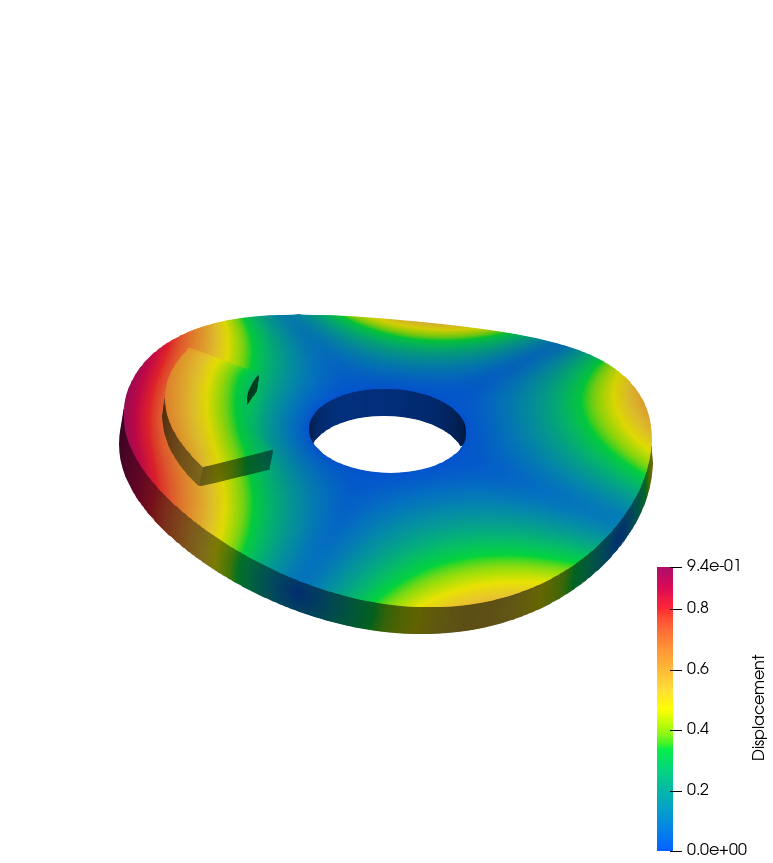
\includegraphics[scale=0.27]{Chapter1/Pictures/Shape_5.png}}
    \subfloat[Mode no. 26, Frequency:9245 Hz]{
    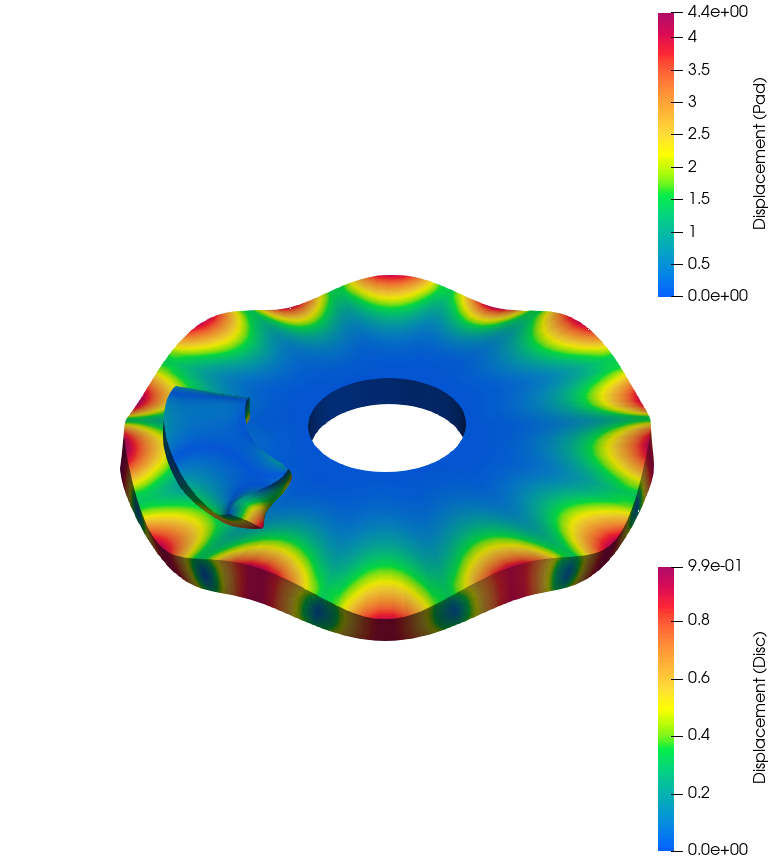
\includegraphics[scale=0.27]{Chapter1/Pictures/Shape_26.png}}
    \caption{Example of disc-pad stable modes}
    \label{fig:stable_modes}
\end{figure}

 \begin{figure}[h!]
    \centering
    \subfloat[Mode no. 45, Frequency:12236 Hz]{
    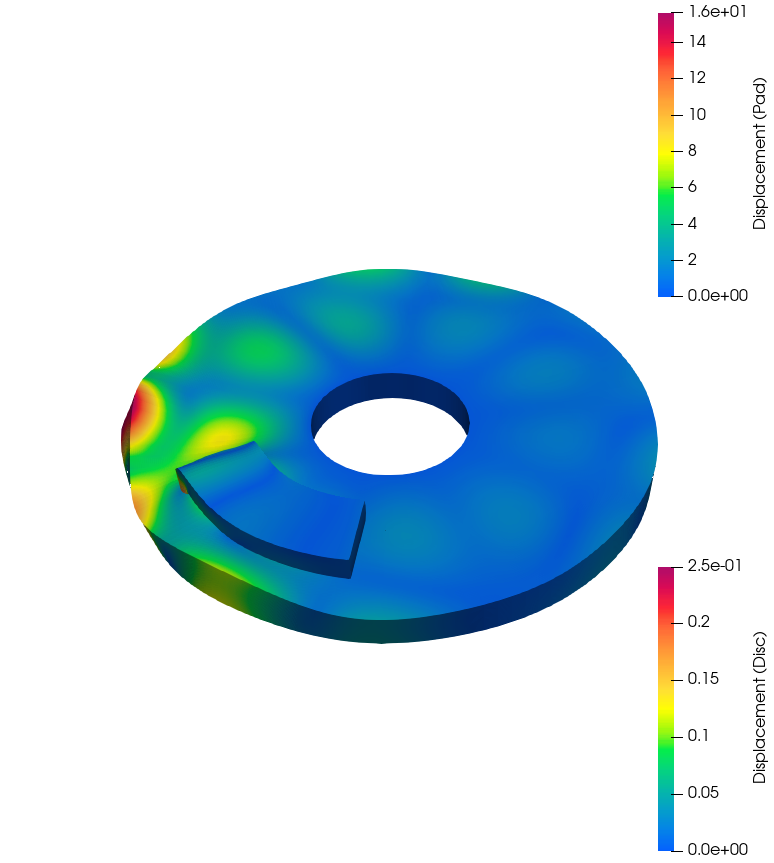
\includegraphics[scale=0.27]{Chapter1/Pictures/Shape_45.png}}
    \subfloat[Mode no. 82, Frequency:17259 Hz]{
    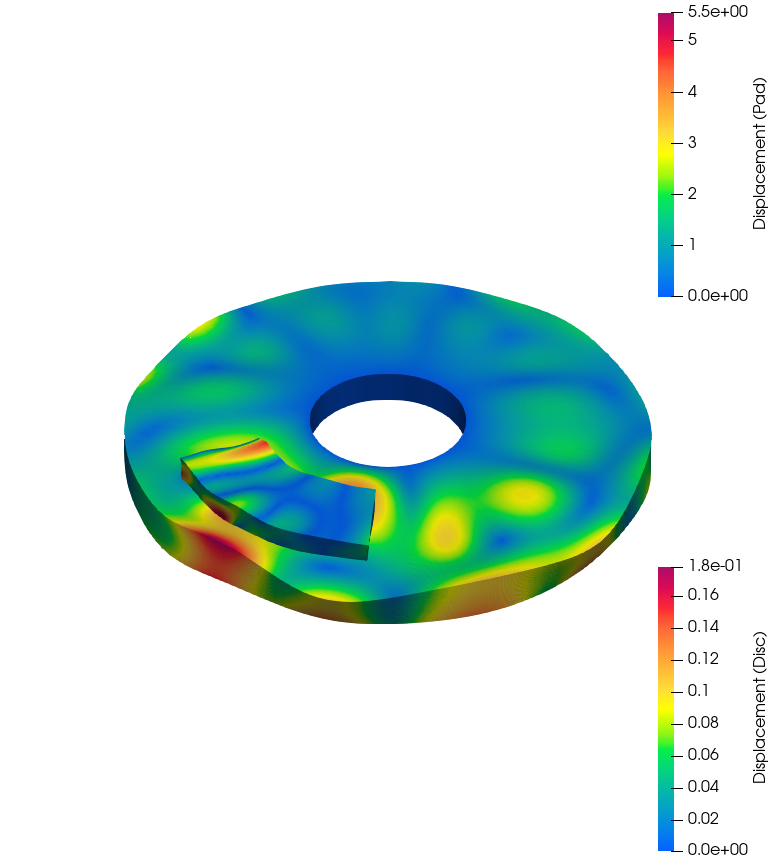
\includegraphics[scale=0.27]{Chapter1/Pictures/Shape_82.png}}
    \caption{Example of disc-pad unstable modes, where the displacement field is considered only for real-part of the eigenvector}
    \label{fig:unstable_modes}
\end{figure}

We discuss the empirical observations from the post-processing of mode shapes, even though the results are highly subjective and depend on the value of $p$ which is typically determined from experiments in the light of normal compliance.
Typically at low frequencies, the mode shape of the pad follows the shape of the disc with correspondence in displacement field at the contact interface. While at higher frequencies, the behaviour is complicated to understand, but relatively large difference in magnitude of displacement field between the disc and the pad was observed. 
Further, the unstable modes lead to definition of eigenvectors in complex-plane for displacement field, which was not considered for representation in Figure \ref{fig:unstable_modes}. 
For intuition, a complex eigenvalue with non-zero real and imaginary parts, defines the phase-lag in the displacement field for an eigenvector and hence, the stable equilibrium position of the displacement field for an eigenvector is never achieved simultaneously.\\

\subsubsection{Optimization criterion definition}

In the context of shape optimization, the idea is to define a criterion for optimization independent of the coefficient of friction ${\mu}$, such as to reduce the influence of ${\mu}$ in determining the shape. This is because the parameter $\mu$ is mostly uncertain in real world and also instabilities could be easily averted at lower values of ${\mu}$. Hence, to define a criterion which characterizes instability for a geometric shape $\bm X$ independent of ${\mu}$, we define the criterion as follows
 
 \begin{equation}
C_{\mathsf s}(\bm X)=\int_{{\mu}} max\{\Re(\bm \Lambda(\bm X,{\mu}))\}\,d{\mu}
    \label{eq:firststabcrit}
\end{equation}
 
where $\bm \Lambda=\{\lambda_1\cdots\lambda_{(.)}\}$ is a set of eigenvalues of the system. 
The criterion is essentially a black-box function defined by the maximum of the real part in $\bm \Lambda(\bm X)$ at a given value of ${\mu}$, integrated over ${\mu}$.
Typically, it can be too unrealistic or optimistic to minimise the criterion over the whole range of squeal frequency ($1$ to $16$ $KHz$) and hence, the set $\bm \Lambda$ can be chosen for a specific range of frequency.
This can also be a better strategy in defining meta-model for $C_{\mathsf s}$, since the meta-model can be more accurate in characterising the behaviour of modes over a specific range of frequency than the whole range.
Even though, no correlation can be implied between $\max\{\Re(\bm \Lambda(\bm X,{\mu}))\}$ and noise level, choosing $\max\{\Re(\bm \Lambda(\bm X,{\mu}))\}$ is essential to define some smoothness for $C_{\mathsf s}$ in optimisation. 
Hence the choice of $\max\{\Re(\bm \Lambda(\bm X,{\mu}))\}$ does not necessarily characterise noise level but the presence of instability which can be accounted for squeal noise. 
Nevertheless, the Utopian goal of $C_{\mathsf s}=0$ defines lack of instabilities and hence characterising noise level may not be a concern if such a goal could be reached in optimisation.\\

Evaluation of $C_{\mathsf s}$ can be computationally expensive, but with the aid of model reduction and parallel computing, it can be made to be efficient. In the following, we give the general frame-work for evaluating $C_{\mathsf s}$.

The reduced stiffness matrices of the multi-patch disc can be defined with C\&B method as

  \begin{equation}
 \mathbf{\hat{K}}^{\mathrm{(d)}}=\left[
\begin{array}{cccc}
  \mathcal{\hat I}^{(\mathrm d)} &0\\
  0&\mathbf{\hat{K}}_{\mathrm{vv}}^{(\mathrm d)} \\
\end{array}
\right] 
 \end{equation}

where the matrix is defined by the coordinates 
$\bm Z^{(\mathrm d)}= \left[\begin{array}{cc}
  \mathscr{M}^{(\mathrm d)} \\
  \bm U_{\mathrm{v}}^{(\mathrm d)} \end{array}\right]$
  , with $\bm U_{\mathrm{v}}^{(\mathrm d)}$ defining the degrees of freedom on $\Gamma_{C}^{(\mathrm d)}$ \footnote{It should be noted that in the context of multi-patch parameterisation, detailed in \S ,$\Gamma_{C}^{(\mathrm d)}$ corresponds to $\Gamma_{C}^{(\mathrm d_1)}$, where the contact interface is defined to be on $\Omega^{(\mathrm d_1)}$.}.
 The matrix is essentially the same in optimisation, when the optimisation is defined only for $\Omega^{\mathrm{p}}$. Hence, for a given definition of shape, the following matrix is computed
 
   \begin{equation}
 \mathbf{\hat{K}}^{\mathrm{(p)}}=\left[
\begin{array}{cccc}
  \mathcal{\hat I}^{(\mathrm p)} &0\\
  0&\mathbf{\hat{K}}_{\mathrm{vv}}^{(\mathrm p)} \\
\end{array}
\right] 
 \end{equation}
 
 The evaluation of $C_{\mathsf s}$ demands the definition of  $\mathbf{\hat{K}}^{\mathrm{(d-p)}}$ for several values of $\mu$. Since $\mu$ is the property of interface, the characteristics at the interface can be decoupled as interface degrees of freedom $\bm U_{\mathrm{v}}$ in C\&B reduced coordinates. For the definition of $\mathbf{\hat K}_F^{\mathrm{(a-b)}}$, $\mu$ can be factored out as  $\mu \mathbf{\hat K}_F^{\mathrm{(a-b)}}|_{\mu=1}$, where in this case with $\mu$ factored out,  $\mathbf{\hat K}_F^{\mathrm{(a-b)}}|_{\mu=1}$ can be interpreted as $\mathbf{\hat K}_F^{\mathrm{(a-b)}}$ computed with $\mu=1$. The idea is that for the evaluation of $C_{\mathsf s}$, with numerical integration defined over $\mu$, the matrix $\mathbf{\hat K}_F^{\mathrm{(a-b)}}$ does not need to be evaluated for discrete values of $\mu$, but instead $\mu$ can be defined as factor of $\mathbf{\hat K}_F^{\mathrm{(a-b)}}|_{\mu=1}$, where $\mathbf{\hat K}_F^{\mathrm{(a-b)}}$ in this case is computed only once with $\mu=1$.\\ 
 
 
The computational cost of evaluating $C_{\mathsf s}$ with numerical integration for discrete values of ${\mu}$ can be reduced through 
 parallel computation. The only varying parameter for parallelisation is $\mu$ for the definition of $\mathbf{\hat K}_F^{\mathrm{(a-b)}}$, hence the computation of the matrices  $\mathbf{\hat{M}}^{\mathrm{(p)}}$, $\mathbf{\hat{K}}^{\mathrm{(p)}}$, $\mathbf{\hat{K}}^{\mathrm{(d-p)}}_C$ and $\mathbf{\hat{K}}^{\mathrm{(d-p)}}_F|_{\mu=1}$ are achieved on single core. Further with $\mathbf{\hat{M}}^{\mathrm{(d)}}$ and $\mathbf{\hat{K}}^{\mathrm{(d)}}$ already computed, the reduced matrices of $\mathbf{\hat{M}}^\mathrm{(d-p)}$ and $\mathbf{\hat{K}}^\mathrm{(d-p)}$ can also be defined on single core as
 
  \begin{equation}
 \mathbf{\hat{M}}^{(d-p)}=\left[
\begin{array}{cc}
  {{\mathbf{\hat M}}}^{(d)} &0\\
  0&{\mathbf{\hat M}}^{(p)} \\
\end{array}
\right] 
 \end{equation}
 

 \begin{equation}
 \mathbf{\hat{K}}^{\mathrm{(d-p)}}_{\uplus C}=\left[
\begin{array}{cccc}
  \mathcal{\hat I}^{(\mathrm a)} &0&0&0\\
  0&\mathbf{\hat{K}}_{\mathrm{vv}}^{(\mathrm a)}+ {{\mathbf{\hat K}}}^{\mathrm{(\mathrm d)}}_C&0&{{\mathbf{\hat K}}}^{\mathrm{(d,p)}}_C \\
  0&0& \mathcal{\hat I}^{(\mathrm p)} &0 \\
  0& {{\mathbf{\hat K}}}^{\mathrm{(p,d)}}_C+{{\mathbf{\hat K}}}^{\mathrm{(p,d)}}_F&0&\mathbf{\hat{K}}_{\mathrm{vv}}^{(p)}+ {{\mathbf{\hat K}}}^{\mathrm{(p)}}_C\\
\end{array}
\right] 
 \end{equation}
 
 
 where the matrices are expressed in coordinates $\mathbf{Z}^{(d-p)}$. Similarly, the matrix $\mathbf{\hat{K}}^{\mathrm{(d-p)}}_F|_{\mu=1}$ can be expressed in  $\mathbf{Z}^{(d-p)}$ coordinates as
 
  \begin{equation}
 \mathbf{\hat{K}}^{\mathrm{(d-p)}}_{\cup F}|_{\mu=1}=\left[
\begin{array}{cccc}
0&0&0&0\\
0& {{\mathbf{\hat K}}}^{\mathrm{(d)}}_F|_{\mu=1}&0& {{\mathbf{\hat K}}}^{\mathrm{(d,p)}}_F|_{\mu=1}\\
0&0&0&0\\
0& {{\mathbf{\hat K}}}^{\mathrm{(p,d)}}_F|_{\mu=1}&0& {{\mathbf{\hat K}}}^{\mathrm{(p)}}_F|_{\mu=1}\\
\end{array}
\right] 
 \end{equation}

The evaluation of $C_{\mathsf s}$ with numerical integration can be expressed as

\begin{equation}
\int_{{\mu}}max\{\Re(\bm \Lambda(\bm X,{\mu}))\}\,d{\mu} \approx \sum_{{\mu}_{\mathsf i}\in [0,1]}max\{\Re(\bm \Lambda(\bm X,{\mu}_{\mathsf i}))\}\,w_{{\mathsf i}}
\end{equation}

where ${\mu}_{\mathsf i}$ can be spaced evenly in the interval $[0,1]$. Hence, on each parallel core, the matrix $ \mathbf{\hat{K}}^{\mathrm{(d-p)}}_{\uplus CF}$ can be computed as

\begin{equation}
\mathbf{\hat{K}}^{\mathrm{(d-p)}}_{\uplus CF} =  \mathbf{\hat{K}}^{\mathrm{(d-p)}}_{\uplus C}+\mu_{\mathsf i} \,\mathbf{\hat{K}}^{\mathrm{(d-p)}}_{\cup F}|_{\mu=1}
\end{equation}

Along with the definition of $\mathbf{\hat{K}}^{\mathrm{(d-p)}}_{\uplus CF}$, the computation in parallel cores is defined for Eq. \eqref{eq:char_eqn} in reduced coordinates, where in each core, the computation of the characteristics eigenvalue problem in reduced coordinates can be expressed as

\begin{equation}
 (\lambda^{2} \mathbf{\hat M}^{\mathrm{(d-p)}}+\mathbf{\hat{K}}^{\mathrm{(d-p)}}_{\uplus C}+\mu_{\mathsf i}\, \mathbf{\hat{K}}^{\mathrm{(d-p)}}_{\cup F}|_{\mu=1}) \Theta =0
\end{equation} 

This eventually leads to the evaluation of $max\{\Re(\bm \Lambda(\bm X,{\mu}_{\mathsf i}))\}$ in each parallel core and hence with the evaluation of  $max\{\Re(\bm \Lambda(\bm X,{\mu}_{\mathsf i}))\}$ on all parallel cores, $C_{\mathsf s}$ can be computed from $\sum_{{\mu}_{\mathsf i}\in [0,1]}max\{\Re(\bm \Lambda(\bm X,{\mu}_{\mathsf i}))\}\,w_{{\mathsf i}}$.


\iffalse
When defined through numerical integration, the criterion demands evaluation at several values of ${\mu}$ and hence is computationally expensive. But this can be evaded through taking advantage of parallel computation with reduced dynamical models using Craig-Bampton reduction, where the computation of the matrices in physical coordinates followed by dynamic model reduction are achieved on the main core. 


The only varying parameter in the parallel cores is $\boldsymbol{\mu}$ and hence, the calculation of the reduced friction matrix $\mathbf{\hat{K}}^f_{d-p}$ matrix --i.e., the reduced matrix  represented in the Craig-Bampton coordinates-- is defined with $\bm{\mu} = 1$ on the main core and the parallelization is defined for distinct values of $\bm{\mu}$ for $\bm{\mu} \mathbf{\hat{K}}^f_{d-p}$. This means that in addition to the definition of $\bm{\mu} \mathbf{\hat{K}}^f_{d-p}$, the computation on the parallel cores is limited to solving the eigenvalue problem \eqref{eq:char_eqn} with the reduced dynamical model for evaluation of the criterion \eqref{eq:firststabcrit}, which makes it computationally efficient.
\fi


\chapter{FEM modelisation}

In classical FEM, typically the elements are constructed from Lagrange polynomials, known as Lagrange elements, where the interpolating polynomials define unity at the nodes. This property means that the nodes lie on the surface discretised by Lagrange elements, which brings the intuition of Node-to-Node contact where the contact is defined between the nodes of conforming meshes at the contact interface. 
Node-to-Node contact can be essentially considered as the collocation method where the strong form of contact or friction definition is satisfied at the nodes in $\Gamma_C$. The area effects can also be partly considered through Isoparametric mapping even though it may not be precise.\\


\iffalse
Even though the factor $c_n$ in the contact integral is determined experimentally in the light of normal compliance approach, the characteristics of  depends on the underlying numerical formulation.

There are some strategies which adapt the collocation scheme to take in to account of area implicitly, where typically contact pressure is correlated to contact stiffness or experimentally determining contact stiffnesses across the contact interface. 
With the former approach of correlating contact stiffness to contact pressure, the contact pressure solved from $\bm{u}_{eq}$ can also be considered as the correlation factor to define contact stiffness for $\bm{\widetilde{u}}$.\\
\fi

Given that we focus on shape optimisation, Node-to-Node contact can place severe constraints in meshing, where structured meshing must be preferred to define confirming meshes at the contact interface. Depending on the design space in shape optimisation, this may not be a very robust strategy, since structured meshing can severely restrict mesh adaptation to avoid distorted elements that can effect the Isoparametric definition of integrals. 
On the other hand, it is well known that unstructured mesh definition may not also lead to robust meshing with classical FEM. 
Due to such complications with meshing, Isogeometric approach can be considered by choosing a robust parameterization strategy which would be rather difficult with classical FEM. 
But also the Node-to-Node contact can not be explicitly defined with Isogeometric approach, since the control points which correspond to nodes in classical FEM may not lie on the surface. 
Rather, the collocation may not have to be on the nodes which is typically preferred in classical FEM, but else where on the surface. 
Hence, the collocation scheme in classical FEM typically defined with Node-to Node contact takes a different form with Isogeometric approach, where the collocation can be defined on the surface or implicitly in the knot span.
We also remind that defining an initial Parametrisation may also be cumbersome with Isogeomtric approach but given a well-defined initial parameterisation, Isogeometric approach can achieve robust refinement.
Although the complications with meshing for classical FEM can be avoided with contact formulations that do not demand confirming meshes at the interface, developing such formulations with Isogeometric approach can be even more advantageous in shape optimisation.\\ 

The effect of contact formulation to the prediction of instabilities with CEA has not been largely studied, where the interest is on the contact characteristics pertaining to the dynamics of the perturbation $\bm{\widetilde{u}}$ rather than $\bm{u}_{eq}$ \eqref{pert_wrt_eq}. 
Nevertheless, we develop a more rigorous formulation with Isogeometric approach in {\color{red} \S}, purely for its advantages in optimisation, where it does not require confirming meshes at the interface -- since also defining confirming meshes can be even more cumbersome with Isogeometric approach due to the tensor product nature of NURBS.\\

We define optimisation of simple shapes through classical FEM discretisation, where the definition of simple shapes vow for a robust structured meshing and hence Node-to-Node contact can be preferred for its simplicity.
With the following explanations, we detail the Node-to-Node collocation method to model the contact and the friction definitions in the problem \eqref{pert_dyn}, where we also show the relation of collocation method to the weak form of contact and friction terms in  \eqref{weak_pert_2}. 
It should be noted that this type of contact and friction definitions are defined with approximations specific for modelling flutter-type dynamic instability with CEA, detailed in {\color{red}\S}.
Considering Eq. \eqref{weak_pert_2}, for classical FEM with Lagrange elements, the space ${}_h \bm V$ is defined by the bases $ {}_h \bm v_i $ of Lagrange polynomials.  





\subsubsection{Contact formulation} \label{weak_pert_2}

The contact definition of the initial-boundary value problem Eq. \eqref{pert_dyn} can be defined in finite element context as

\begin{equation}
{}_h\sigma^{(\mathrm k)}_n({}_h\bm{\widetilde u}^\mathrm{(k)}) = - \mathit{p}{{}_h\widetilde{u}_n}^{(\mathrm k)} \quad \mathrm{on}\quad\Gamma^{\mathrm{(k)}}_C\\
\end{equation}

where for a system with two domains $\Omega^{(a)}$ and  $\Omega^{(b)}$ in contact. 
With confirming mesh at $\Gamma_C^{(a)}$ and $\Gamma_C^{(b)}$, it can be said that for any node ${i} \in \Gamma_C^{(\mathrm a)}$, there exists a unique node ${j} \in \Gamma_C^{(\mathrm b)}$ that forms contact. Hence, the contact force for a given node $i \in \Gamma_C^{\mathrm (a)}$ in contact with a node $j \in \Gamma_C^{\mathrm (b)}$ can simply be expressed with Node-to-Node contact as

\begin{equation}
  \mathit{p}({{}_h\widetilde{\bm u}}^{(\mathrm a)} - {{}_h \widetilde{\bm u}}^{ ( \mathrm b)}). \bm{\hat{\mathrm v}}_n\bigg|_{ {}_h \bm v_i^\mathrm{(a)}= {}_h \bm v_i^\mathrm{(b)}=1}  = p ( \widetilde{ \bm u}_{{i}}^{(\mathrm a)}- \widetilde{ \bm u}_{{j}}^{(\mathrm b)}). \bm{\hat{\mathrm v}}_n = {}_ht^{(\mathrm k)}_n
\end{equation}

where ${{}_h\widetilde{\bm u}}^{(\mathrm a)} = \sum_{\forall {i} \in \Omega^{(\mathrm a)}} {}_h\bm v_i^\mathrm{(a)} \widetilde{\bm u}_i^\mathrm{(a)}$ and ${{}_h\widetilde{\bm u}}^{(\mathrm b)} = \sum_{\forall {j} \in \Omega^{(\mathrm b)}} {}_h\bm v_j^\mathrm{(b)} \widetilde{\bm u}_j^\mathrm{(b)}$. Since the collocation is defined at the nodes itself, the bases ${}_h \bm v_i^\mathrm{(a)}= {}_h \bm v_i^\mathrm{(b)}=1$ for Lagrange elements or typically for elements in classical FEM. The above equation is stated specifically for linear case, where normal compliance terms are expressed to be linear.\\

As an alternate interpretation, the collocation method can also be defined from the weak form of contact \eqref{pert_cont} as

\begin{multline}
{\langle {}_h \bm{\sigma}^{\mathrm{(a)}}_n, {}_h \bm v_i^\mathrm{(a)} \rangle_{\Gamma_C^{\mathrm{(a)}}}} =\int_{\Gamma^{(a)}_C}  \mathit{p}[({{}_h\widetilde{\bm u}}^{(\mathrm a)} - {{}_h \widetilde{\bm u}}^{ ( \mathrm b)}). \bm{\hat{\mathrm v}}_n]  {}_h \bm v_i^\mathrm{(a)}. \bm{\hat{\mathrm v}}_n \,\,d{\Gamma^{(\mathrm a)}_C}
\rightarrow\\ 
p ( \widetilde{ \bm u}_{{i}}^{(\mathrm a)}- \widetilde{ \bm u}_{{j}}^{(\mathrm b)}). \bm{\hat{\mathrm v}}_n\end{multline}

if the weighting function $ {}_h \bm v_i^\mathrm{(a)}$ of the weak form is defined to be the Dirac-delta function $(\delta_D(.))$ as $ {}_h \bm v_i^\mathrm{(a)} = \delta_D(\widetilde{ \bm u}_{{i}}^{(\mathrm a)} - \widetilde{ \bm u}^{(\mathrm a)})$ \footnote{$ \delta_D(\widetilde{ \bm u}_{{i}}^{(\mathrm a)} - \widetilde{ \bm u}^{(\mathrm a)}): {}_h \bm v_i^\mathrm{(a)} = 0, \,\, \forall \widetilde{ \bm u}_{{i}}^{(\mathrm a)} \neq \widetilde{ \bm u}^{(\mathrm a)}$ and ${}_h \bm v_i^\mathrm{(a)} = 1$ if $\widetilde{ \bm u}_{{i}}^{(\mathrm a)} = \widetilde{ \bm u}^{(\mathrm a)}$}.\\


As aforementioned, we do not focus on the physical characteristics of contact stiffness in the light of normal compliance, and its subsequent effect on CEA, where we define contact stiffness purely as a penalty coefficient $p$. 
But to proceed with the following discussions, we must make a strong assumption on the existence of global contact stiffness ($p_{G}$) such that this property is independent of the contact interface area. 
This is because, if $p$ is a parameter of differential area determined from experiments, it cannot be taken in to account with Node-to-Node contact unless area is implicitly considered. This is largely the case if contact stiffness has correlation with contact pressure at the interface. 
%This is also important to eliminate bias of contact stiffness in optimisation. 
%With this assumption, This is to eliminate bias in optimisation, where larger area can have larger contact stiffness globally relative to a shape with smaller contact area. 
%Hence, we implicitly make a strong assumption that contact stiffness is property associated globally. 
%This can also be interpreted as $p_{G}$  being associated with net force, while local contact stiffness ($p_{l}$) being associated with pressure, which may not be necessarily true.  
 It is only safe to say that experimental studies can alone determine if $p$ is a global or local parameter, such that to eliminate any bias of contact stiffness in defining instability for shape optimisation. 
Nevertheless, with this strong proposition, contact stiffness between any two spatially corresponding nodes is defined by local contact stiffness $p_{l}$, defined as 
   
\begin{equation}
p_{l} = \frac{p_G}{\mathrm{m}}
\end{equation}\\

where ${\mathrm{m}}$ is the number of contact nodes at the interface.
%The convergence of the stability criteria $C_s$ for a given design point based on the choice of the number of contact pairs is also discussed in \S.\\

Similarly, the friction definition of the initial-boundary value problem Eq. \eqref{pert_dyn} can be defined in finite element context as 

\begin{equation}
{}_h\sigma^{(\mathrm k)}_t({}_h\bm{\widetilde u}^\mathrm{(k)}) = \mu \mathit{p}{{}_h\widetilde{u}_n}^{(\mathrm k)} \quad \mathrm{on}\quad\Gamma^{\mathrm{(k)}}_C\\
\end{equation}

Similar to the definition of contact force, the tangential force of friction can be defined with Node-to-Node collocation as 

\begin{equation}
  \mu \mathit{p}({{}_h\widetilde{\bm u}}^{(\mathrm a)} - {{}_h \widetilde{\bm u}}^{ ( \mathrm b)}). \bm{\hat{\mathrm v}}_n\bigg|_{ {}_h \bm v_i^\mathrm{(a)}= {}_h \bm v_i^\mathrm{(b)}=1}  = \mu p ( \widetilde{ \bm u}_{{i}}^{(\mathrm a)}- \widetilde{ \bm u}_{{j}}^{(\mathrm b)}). \bm{\hat{\mathrm v}}_n
\end{equation}

where vectorially, the friction force can be expressed as $\mu [p ( \widetilde{ \bm u}_{{i}}^{(\mathrm a)}- \widetilde{ \bm u}_{{j}}^{(\mathrm b)}). \bm{\hat{\mathrm v}}_n]\bm{\hat{\mathrm v}}_t$, with $\bm{\hat{\mathrm v}}_t$ for a given node being known a priori. For the $d-p$ system, the friction force can be resolved in to tangential and radial components relative to the disc axis. Since, the relative sliding velocity is negligible in the radial direction, the frictional force component of the radial direction is also negligible and hence often ignored. 

\iffalse
\subsubsection{Model reduction}

The evaluation of the stability criterion $C_s$ involves expensive computation for eigenvalues evaluated at various friction coefficients to capture the evolution of the instability. While only the major unstable modes constituting the squeal noise is required to be identified, the model can be simplified by dynamic model reduction techniques. This further allows us to simplify the damping definition of the dynamic model with the method of modal damping. The method of Craig \& Bampton reduction is applied to the model, which is considered to be effective since it captures the dynamic properties at the contact interface and also the internal dynamic properties of the models involved in contact. More detailed description of Craig \& Bampton method used in brake squeal application can be found in literature \cite{BESSET2017896} and \cite{MONTEIL20161073}.   In accordance with the Craig \& Bampton theory,

\begin{equation}
\bm U=\left\{
\begin{array}{c}
     {\bm U}_i  \\
     {\bm U}_j 
\end{array}\right\};
\quad
\bm K=\left[
\begin{array}{cc}
  {\bm K}_{ii} &{\bm K}_{ij} \\
  {\bm K}_{ji} &{\bm K}_{jj} \\
\end{array}
\right];
\quad
\bm M=\left[
\begin{array}{cc}
  {\bm M}_{ii} &{\bm M}_{ij} \\
  {\bm M}_{ji} &{\bm M}_{jj} \\
\end{array}
\right]
%\left[
%\begin{array}{cc}
%{\bm U_i}\\
%{\bm U_j}\\
%\end{array}
%\right]
%=
%\left[
%\begin{array}{cc}
%F_i\\
%F_j\\
%\end{array}
%\right]
\end{equation}\\

where $\bm U_i$ and $\bm U_j$ are internal and interface degrees of freedom respectively. The transformation matrix $\bm T$ is defined as composition of static transformation ${\bm \Phi}_s$ and Eigen vectors ${\bm \Phi}_d$, as follows\\

\begin{equation}
{\bm T}=
\left[
\begin{array}{cc}
  {\bm \Phi}_d &{\bm \Phi}_s \\
  \bm 0 & \bm I \\
\end{array}
\right];
\quad
{\bm\Phi}_s={\bm K}_{ii}^{-1} {\bm K}_{ij};
\quad
{\bm \Phi}_d=[\Phi_0,\Phi_1,...,\Phi_n]\
\end{equation}\\


where $\Phi_n$ is the $n^\text{th}$ eigenvector obtained from the eigenvalue problem defined as $({\bm K}_{ii}-\omega_n^2{\bm M}_{ii})\Phi_n=0$. The choice of the number of eigenvectors $n$ considered for reduction depends on the convergence required with respect to prediction of the eigenvalues for the unstable modes obtained by the reduced model.\\

The reduced mass matrix ${\bm  M}_{r}$ and stiffness matrix ${\bm  K}_{r}$ are respectively obtained through the transformation matrix ${\bm T}$ applied as ${\bm T}^t{\bm  M}_{s}{\bm T}$ and ${\bm T}^t{\bm  K}_{s}{\bm T}$, where ${\bm  K}_{s}$ is the stiffness matrix of the system with friction definition. The matrix ${\bm  K}_{r}$ is largely uncoupled, defined in the modal coordinates, except for the non-diagonal terms which can be viewed as the terms constituting the effects of friction in the modal coordinates and also the part of the matrix with static reduction is non-diagonal. While the reduction of the mass matrix from ${\bm  M}_{s}$ to ${\bm  M}_{r}$ is simply straight forward.\\

The Craig-Bampton reduction leads to reduced matrices of size ${\bm[\;S\times S\;]}$, where $\bm S$ is given by the sum of the number of contact points at the system interface and the number of eigenvectors of the system considered. This greatly reduces the computation time of the Complex eigenvalue analyses for the estimation of the stability criteria. \\

\fi


\subsubsection{Mesh sensitivity}

In relation to the expensive evaluation of the stability criteria, mesh convergence study was performed for the influence of mesh at the contact interface and outside the contact interface. The eigenmodes reflecting maximum instability as predicted by the maximum positive real part of the complex eigenvalues are only of interest to us and hence taken in to account to check for convergence. It should be noted that the contact formulation can have some influence on mesh convergence especially for CEA, where no clear studies has been performed. In this case, we are specific for convergence with for node-to-node formulation. \\

The dynamic properties with respect to maximum instability show little variation for change in mesh size out of the contact region for a given shape and number of contact points. The comparison is shown through a model with highly coarse mesh as in Fig. \ref{fig:coarse_mesh} against  a model with the same shape but for a relatively fine mesh as in Fig. \ref{fig:h_mesh}, while maintaining the same number and position for the contact points. The mismatch in frequencies between the models is shown in Fig. \ref{fig:h_freq} where the range for frequency is zoomed to a pair of frequencies which induce mode coalescence predicted to cause the maximum instability. The shift in unstable frequencies and the point of bifurcation of the maximum real part as shown in Fig. \ref{fig:h_real} are observed to be very low for change in mesh size.\\


\begin{figure}
    \centering
    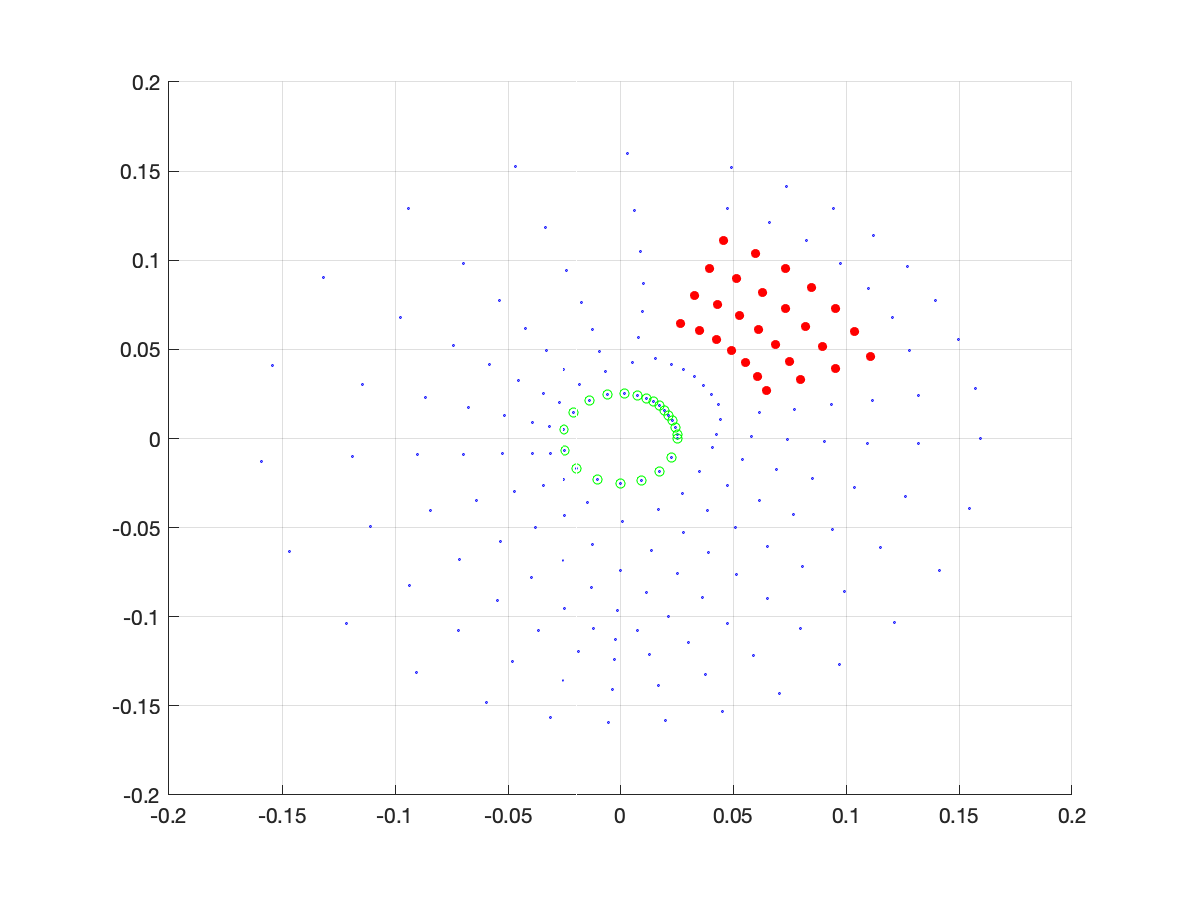
\includegraphics[scale=0.43]{Chapter2/Pictures/Geo_pub_h1.eps}
    \caption{Node plot for a coarse mesh of the disc geometry with contact nodes represented in red}
    \label{fig:coarse_mesh}
\end{figure}

\begin{figure}
    \centering
    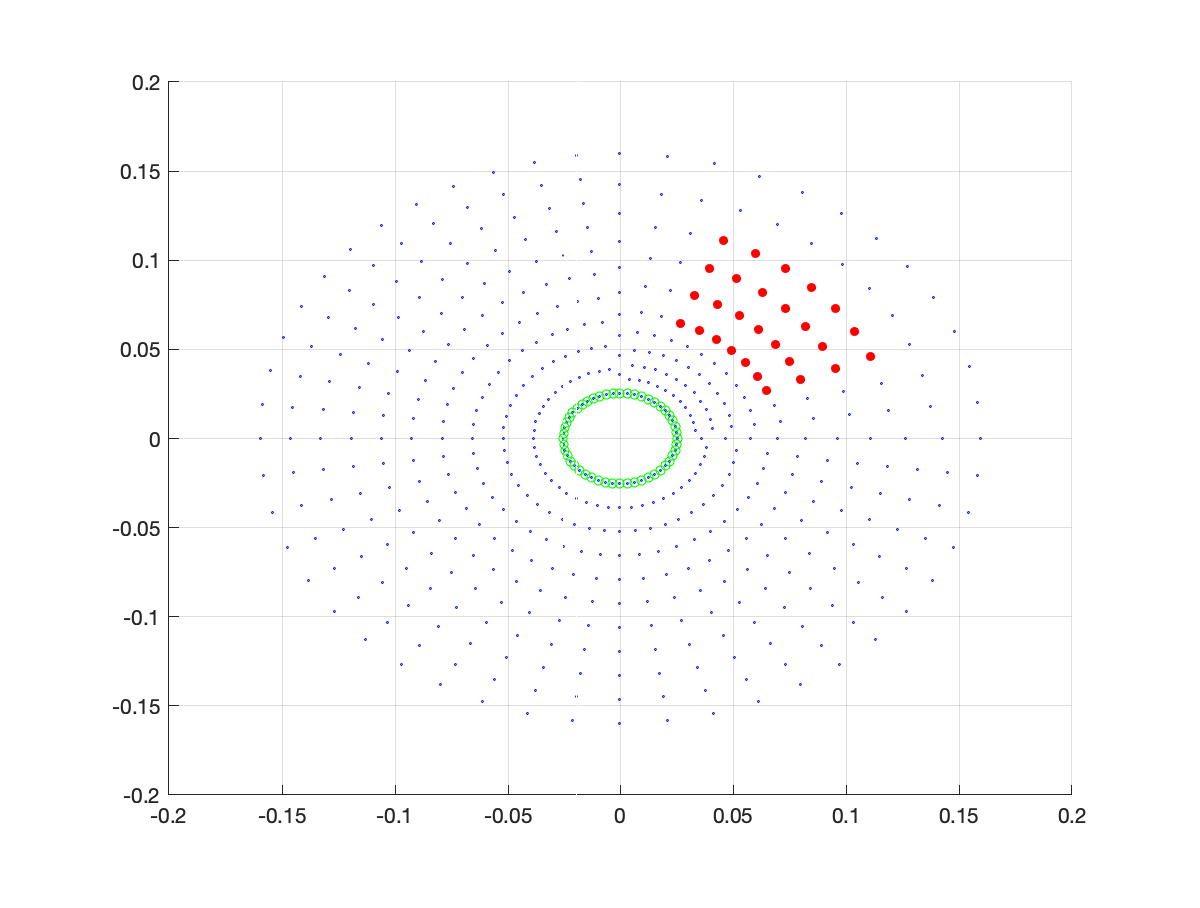
\includegraphics[scale=0.43]{Chapter2/Pictures/Geo_pub_h.eps}
    \caption{ Node plot for a relatively fine structured mesh of the disc geometry with contact nodes represented in red}
    \label{fig:h_mesh}
\end{figure}

\begin{figure}
    \centering
    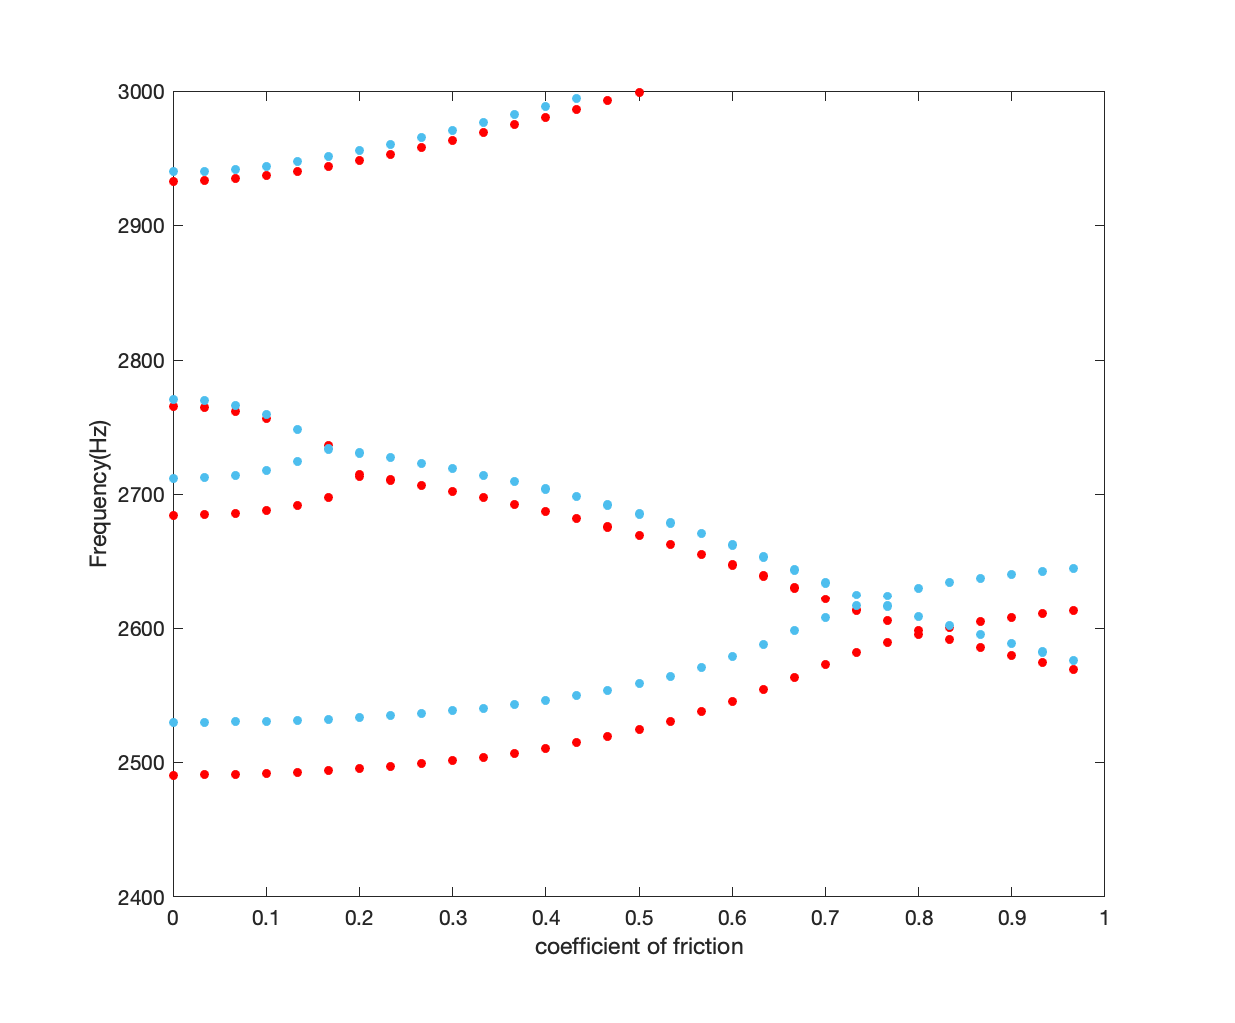
\includegraphics[scale=0.43]{Chapter2/Pictures/hvsh1_freq1.eps}
    \caption{Plot of Frequency vs Friction coefficient, of modes showing maximum instability; Blue represents for the model in \ref{fig:coarse_mesh}; Red represents for the model in \ref{fig:h_mesh}}
    \label{fig:h_freq}
\end{figure}

\begin{figure}
    \centering
    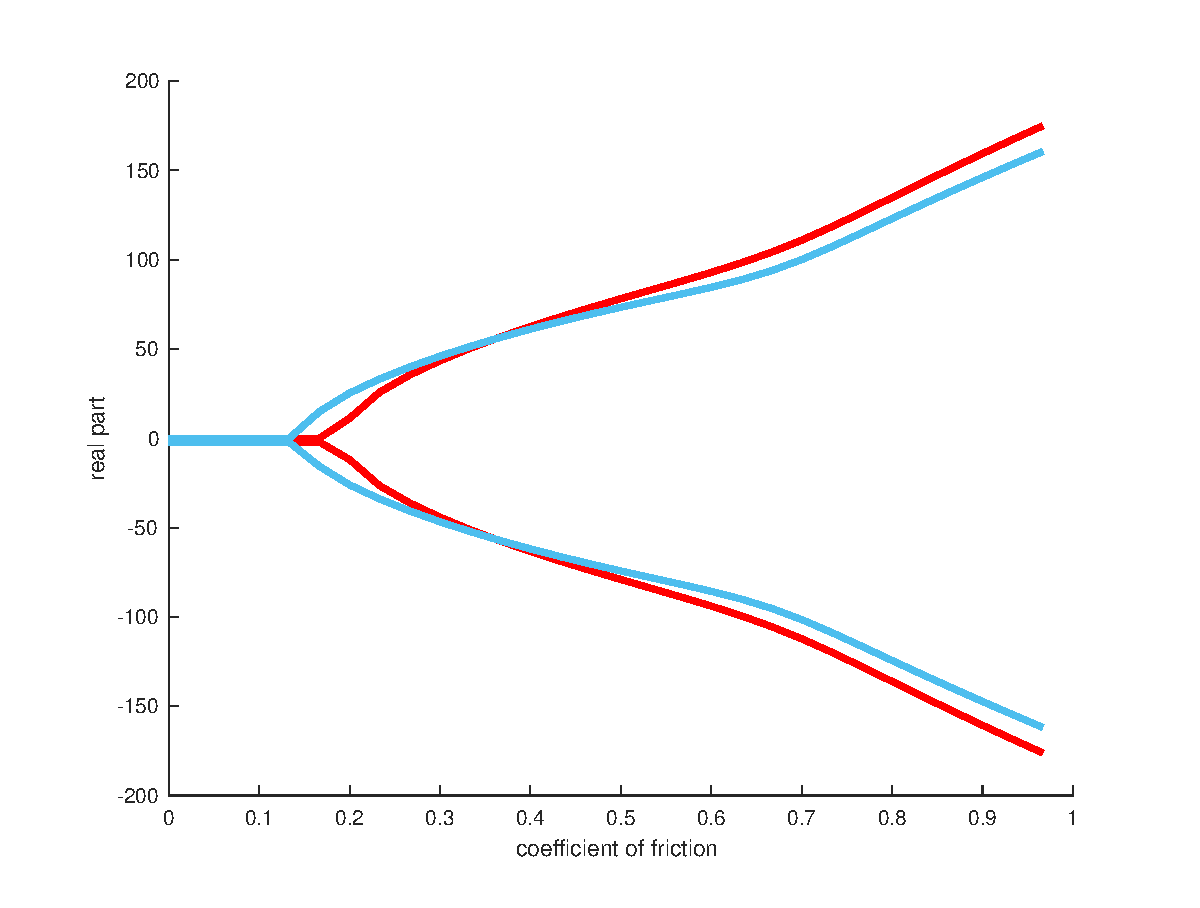
\includegraphics[scale=0.43]{Chapter2/Pictures/hvsh1_real.eps}
    \caption{Plot of Real part of the complex eigenvalues vs Friction coefficient, of modes showing maximum instability; Blue represents for the model in \ref{fig:coarse_mesh}; Red represents for the model in \ref{fig:h_mesh}}
    \label{fig:h_real}
\end{figure}

Though the variation of the mesh out of the contact interface is shown to have a little influence on the maximum instability, the variation of mesh at the contact interface is observed to have a considerable effect on the dynamic properties. This can be seen by comparing results of the models in Fig. \ref{fig:coarse_mesh} and Fig. \ref{fig:h_mesh} against the models in Fig. \ref{fig:hh_mesh} and Fig. \ref{fig:hhhh_mesh} which are of the same shape. Hence, it is intuitive to assume a large number of contact points, since the contact interface is a continuum after all. The convergence is shown with large number of contact points in Fig. \ref{fig:hh_mesh} and Fig. \ref{fig:hhhh_mesh} with plot for bifurcation of the real part in Fig. \ref{fig:hhhh_real}) and frequencies inducing maximum instability in Fig. \ref{fig:hhhh_freq}. \\

\begin{figure}
    \centering
    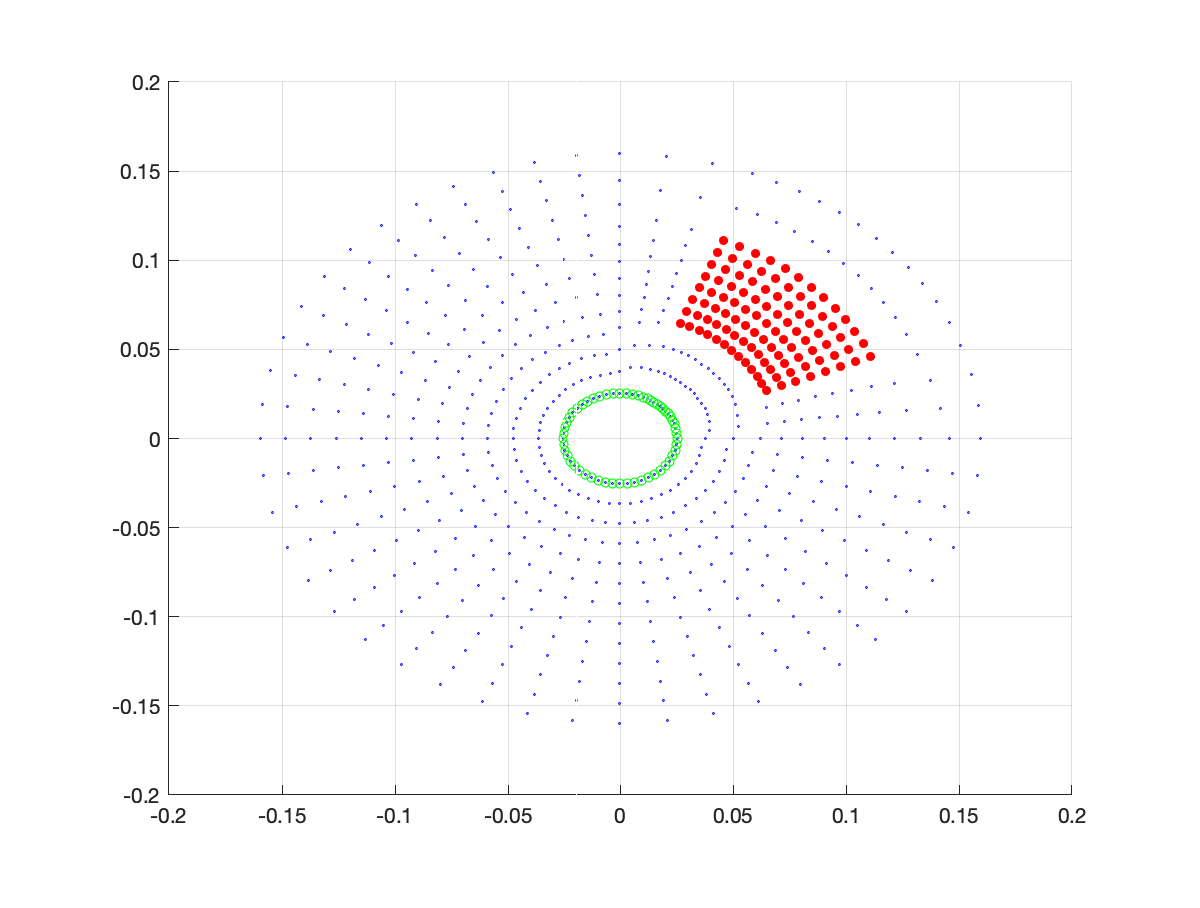
\includegraphics[scale=0.43]{Chapter2/Pictures/Geo_pub_hh.eps}
    \caption{Node plot for a fine mesh with contact nodes represented in red}
    \label{fig:hh_mesh}
\end{figure}

\begin{figure}
    \centering
    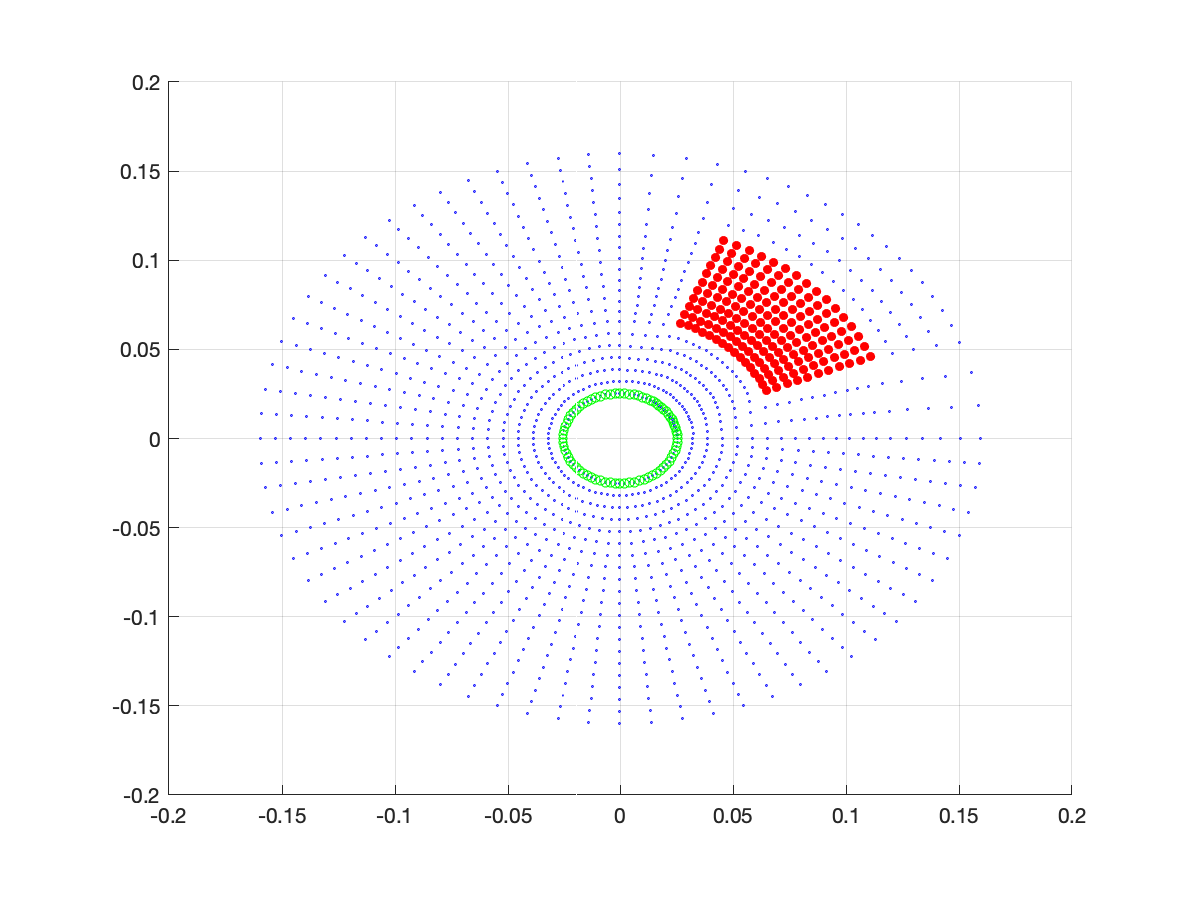
\includegraphics[scale=0.43]{Chapter2/Pictures/Geo_pub_hhhh.eps}
    \caption{ Node plot for a relatively finer mesh compared to \ref{fig:hh_mesh}, especially on the contact interface with contact nodes represented in red}
    \label{fig:hhhh_mesh}
\end{figure}

\begin{figure}
    \centering
    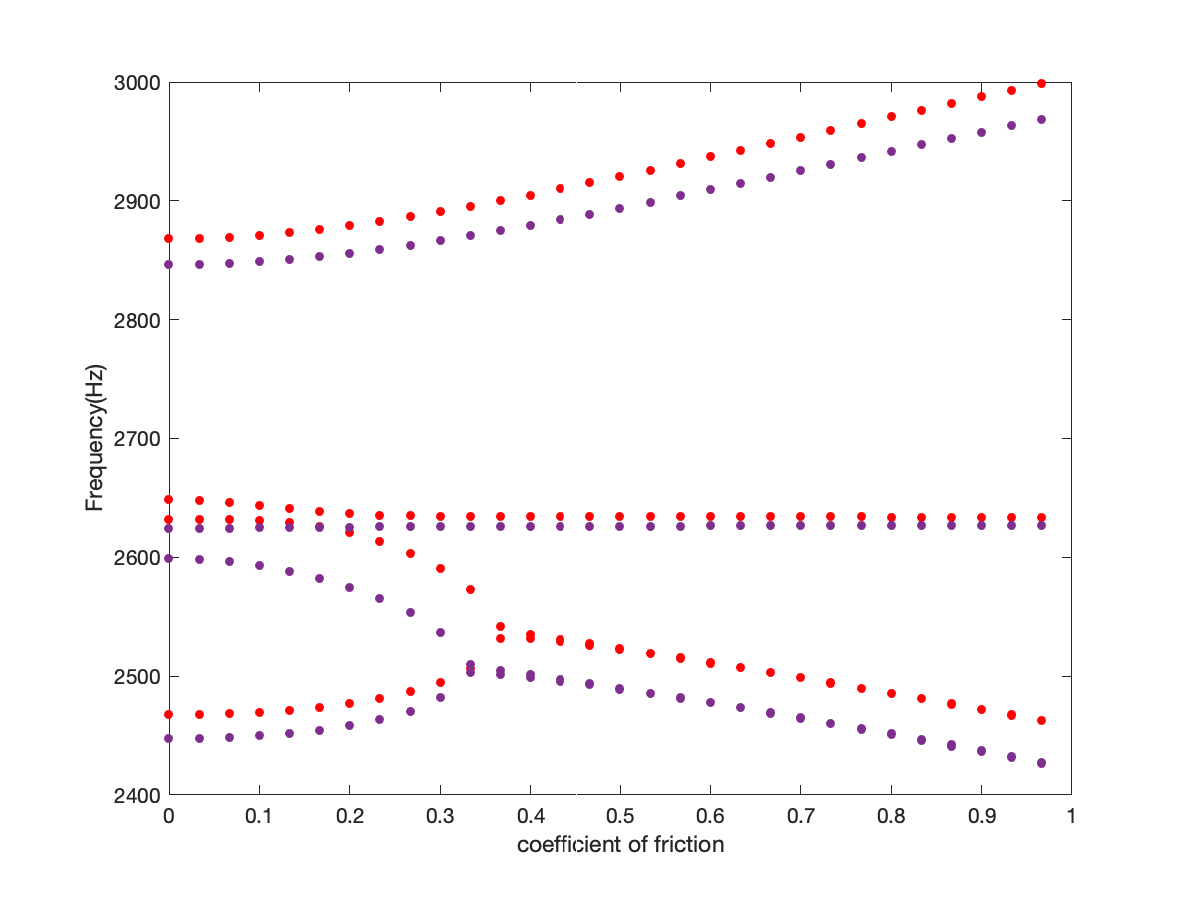
\includegraphics[scale=0.43]{Chapter2/Pictures/hhvshhhh_freq.eps}
    \caption{Plot of Frequency vs Friction coefficient, of modes showing maximum instability; Red represents the plot for the model in \ref{fig:hh_mesh}; Violet represents the plot for the model in \ref{fig:hhhh_mesh}}
    \label{fig:hhhh_freq}
\end{figure}

\begin{figure}
    \centering
    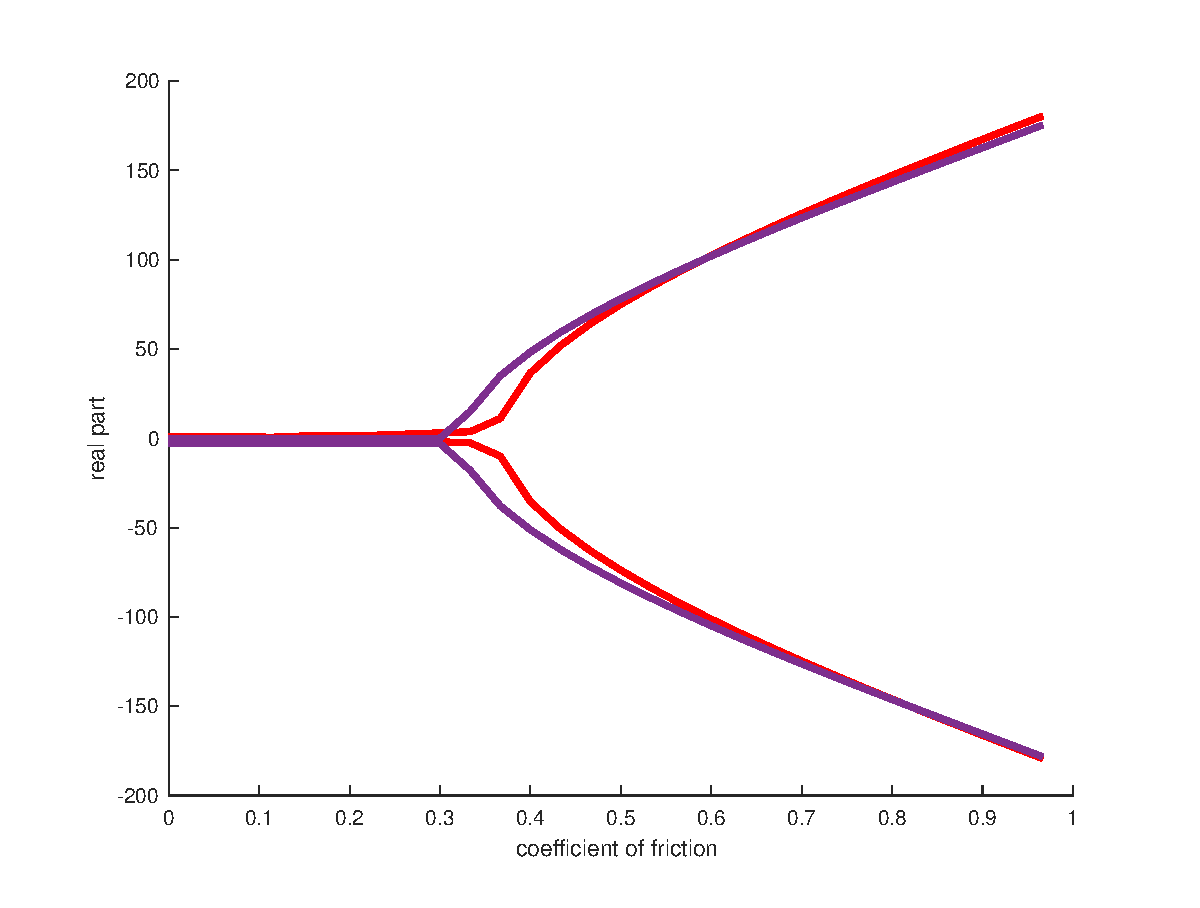
\includegraphics[scale=0.43]{Chapter2/Pictures/hhvshhhh_real.eps}
    \caption{Plot of Real part of the complex eigenvalues vs Friction coefficient, of modes showing maximum instability; Red represents the plot for the model in \ref{fig:hh_mesh}; Violet represents the plot for the model in \ref{fig:hhhh_mesh}}
    \label{fig:hhhh_real}
\end{figure}

The definition of the contact points can be observed to have significant influence on the maximum real part of the complex eigenvalues and hence also the stability criteria, which demands a good mesh definition to define a robust stability criteria in optimisation. For this reason, we defined a structured mesh as in Fig. \ref{fig:disc_mesh} where linear hexahedral elements are largely used through out the model with smaller elements at the contact interface, while the region outside of contact interface is defined by larger elements. The difference in mesh density is compromised by introducing 3D wedge elements to maintain a structured mesh.\\ 


\begin{figure}
    \centering
    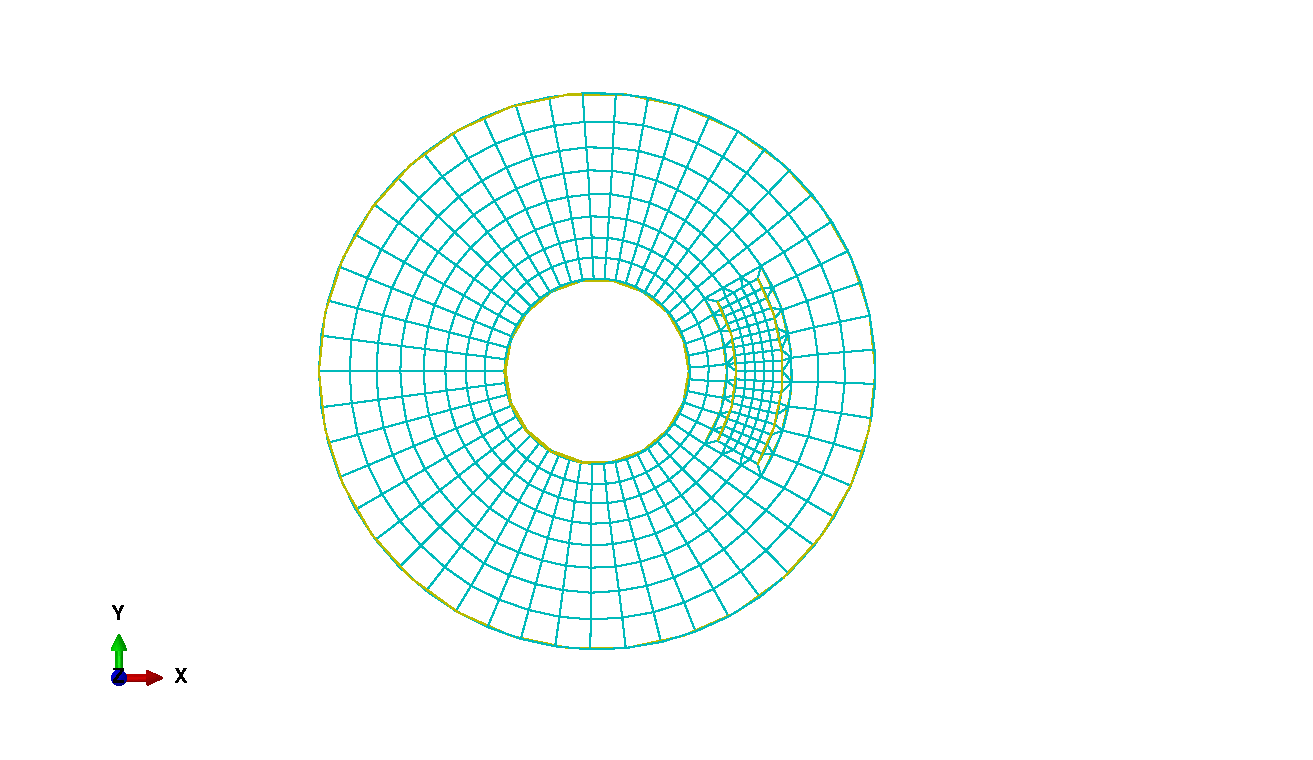
\includegraphics[scale=0.6]{Chapter2/Pictures/disc1.eps}
    \caption{Considered mesh definition}
    \label{fig:disc_mesh}
\end{figure}






\chapter{IGA formulation}
\cite{ha2015}
We start with the definition of B-spline functions with extension to B-spline curves, from which NURBS curves are introduced with the definition of a weighing parameter and a non-uniform knot vector. This is followed by description of higher dimensional geometries through extension by tensor product definition.\\
 
 The B-spline basis functions can be defined by Cox de Boor's formula as follows,
 
\begin{equation}
{N_{i,0}\left( \xi  \right)} = \left\{ {\begin{array}{cl}
   1 & {\;{\xi _i} \le \xi  < {\xi _{i + 1}}}  \\
   0 & {\;otherwise}
\end{array}} \right.
\end{equation}

\begin{equation}
{N_{i,p}\left( \xi  \right)} = \frac{{\xi  - \xi_{i} }}{{{\xi _{i + p}} - {\xi _i}}}{N_{i,p - 1}\left( \xi  \right)} + \frac{{{\xi _{i + p + 1}} - \xi }}{{{\xi _{i + p + 1}} - {\xi _{i + 1}}}}{N_{i + 1,p - 1}\left( \xi  \right)}
\end{equation}

where $p$ is defined recursively for $p>0$ to obtain a curve of degree $p$, which starts with a piecewise constant at $p=0$. Naturally, a uniform knot vector can be defined as  $\bm \xi  = \left\{ {{\xi _1},{\xi _2}, \cdots ,{\xi _{n + p + 1}}} \right\}$, where any $\xi_i - \xi_{i+1}$ is uniformly spaced.  
For a uniform knot vector, the bases span with continuity $C^{p-1}$ between the knots, where it satisfies partition of unity $\sum_{i=1}^{n} {N_{i,p}\left( \xi  \right)} = 1$ for $[\xi _p,\xi _{n+1}]$, with $n$ being the number of control points. Further, the span of any ${N_{i,p}\left( \xi  \right)}$ is defined in $[\xi_i,\xi_{i+p+1}]$, and ${N_{i,p}\left( \xi  \right)} \geq 0$, $\forall \xi$.\\

The knot vector need not be equidistant and the multiplicity  of a knot $\xi _i$ by $\mathcal{M}$ in the knot vector decreases the continuity by $C^{p-\mathcal{M}}$ across the knot $\xi _i$,  which defines a non-uniform knot vector. 
The multiplicity $\mathcal{M}=p$ for the first knot and the last knot defines a open knot vector, where the basis functions model interpolation between the first and the last knots. 
The basis functions defined with an open knot vector satisfies partition of unity $\forall \xi$. 
Through B-spline basis functions and a knot vector $\bm \xi  = \left\{ {{\xi _1}, \cdots ,{\xi _{n + p + 1}}} \right\}$, a B-spline curve can be defined with coefficients of the basis functions as follows 

\begin{equation}
\bm X_c(\xi) =  \sum_{i=1}^n N_{i,p}(\xi)  \bm {{P}}_i
\end{equation}

where with a open knot vector for a curve, the ends of the curve are $C^0$. The coefficients $\bm{{P}}_i \in \mathbb{R}^{d}$ are the control points, with $d$ being the dimension of the space. The definition of a weighing parameter $w_i >0$ associated with a re spective basis function $N_i$, normalized defines rational B-splines where it respects the partition of unity, given as follows
\begin{equation}
\bm X_c(\xi) =  \sum_{i=1}^n\underbrace{\frac{w_iN_{i,p}(\xi)}{\sum_{i=0}^n{w_iN_{i,p}(\xi)}}}_{R_{i,p}}\bm {{P}}_i \label{NURBS_c}
\end{equation}

The parameter $w_i$ provides a new dimension for controlling the geometry through projective transformation, while the affine transformation is achieved by $\bm{{P}}_i$ . Hence, the combination of non-uniform knot vectors and rational basis functions define NURBS. Further, if all weights are the same, NURBS is simply a B-spline with non-uniform knot vector.\\

%Add figure for projective trans IGA book

The higher dimensional NURBS are a natural extension of its $1$-dimensional precursor through tensor product definition where the order of the tensor is the same as the dimension of the geometry. For a $2$-dimensional geometry, the tensor product NURBS surface is defined as follows

\begin{equation}
\bm X_s(\xi,\eta) =   \sum_{i=1}^n\sum_{j=1}^m  R_{i,p}(\xi)R_{j,q}(\eta)\bm{{P}}_{i,j} \label{NURBS_s}
\end{equation}

which is supported by knot vectors $\bm \xi = \left\{ {{\xi _1}, \cdots ,{\xi _{n + p + 1}}} \right\}$ and $\bm \eta = \left\{ {{\eta _1}, \cdots ,{\eta _{m + q + 1}}} \right\}$, for the domain $[\xi_1,\xi_{m+q+1}] \times [\eta_1,\eta_{m+q+1}]$, with $n\times m$ net of control points $\bm{{P}}_{i,j}$. Similarly, to define volume, the tensor product NURBS volume is defined as follows

\begin{equation} \label{NURBS_v}
\bm X_v(\xi,\eta,\zeta) =   \sum_{i=1}^n\sum_{j=1}^m\sum_{k=1}^l  \underbrace{R_{i,p}(\xi)R_{j,q}(\eta)R_{k,r}(\zeta)}_{R_{i,j,k}(\mathbf{\Xi})}\bm {{P}}_{i,j,k}
\end{equation}

where the knot vectors are given as $\bm \xi = \left\{ {{\xi _1}, \cdots ,{\xi _{n + p + 1}}} \right\}, \bm \eta = \left\{ {{\eta _1}, \cdots ,{\eta _{m + q    + 1}}} \right\}$ and $\bm \zeta = \left\{ {{\zeta _1}, \cdots ,{\zeta _{l + r + 1}}} \right\}$. \\

The above expression can be simply expressed in matrix form as $\bm X_v(\mathbf{\Xi}) = \mathbf{R(\Xi) \mathbf{P}}$. 

where,

$\mathbf{R(\Xi)}$

\subsubsection{IGA discretization}\label{IGA_contandfric}

We defined the general view of the space ${}_h \bm V$ and now we give a more precise definition of the space with the Isogeometric approach. The main idea with Isogeometric approach is to define ${}_h \bm V$ as the space of the NURBS basis functions which also parameterizes the geometry. 
The parameterization of a domain $\Omega \in \mathbb{R}^3$ as an initial geometric description through NURBS can be defined as $\breve{\bm {X}}^\mathrm{(k)}_v(\breve{\mathbf{\Xi}}^\mathrm{(k)}) = \breve{{\mathbf{R}}}^\mathrm{(k)} (\breve{\mathbf{\Xi}}^\mathrm{(k)}) \breve{\mathbf{P}}^\mathrm{(k)}$, $\bm X : \hat{\Omega}\rightarrow\Omega$, where $\bm {X}$ defines the mapping from the parametric domain $\hat{\Omega}$ to the physical domain $\Omega$ -- for simplicity, we consider the parameterization of the domain $\Omega_\mathrm{k}$  through a single patch: $[ {\xi _1}, \cdots ,{\xi _{n + p + 1}} ] \times  [ {{\eta _1}, \cdots ,{\eta _{m + q    + 1}}} ] \times [ {\zeta _1}, \cdots ,{\zeta _{l + r + 1}} ]$ . 
The analysis-suitable parameterization $\bm X$ \footnote{For simplicity of the notation, we define $\bm{X}$ to be the default notation for analysis-suitable parameterization of a domain $\Omega \in \mathbb{R}^3$} can be achieved through the refinement of $\breve{\bm{X}} \rightarrow \bm{X}$ with one or several of the refinement methods ($h$, $p$ and $k$), where $\bm X$ can be defined as ${\bm {X}}_v({\mathbf{\Xi}}) = {\mathbf{{R}}}(\mathbf{\Xi}) \mathbf{{P}}$ to take in to account of the modified knot vectors and control points -- more on parameterization and refinement for our applicative example of disc-pad system is discussed in.\\

The Isogeometric approach for approximation of the solution $\bm{u}_\mathrm{k}$ is achieved through the same NURBS bases $R_{i,j,k}$, where for the vector-valued function space ${}_h\bm V$, the vectorial definition of the bases  $\bm R_{i,j,k} \in \mathbb{R}^3$ can be defined as\\

$ \begin{Bmatrix}
\begin{bmatrix}
 R_{i,j,k}\\ 
 0\\
 0  
\end{bmatrix}\\ 
\end{Bmatrix}
\bigcup
\begin{Bmatrix}
\begin{bmatrix}
 0\\ 
 R_{i,j,k}\\
 0  
\end{bmatrix}\\ 
\end{Bmatrix}
\bigcup
\begin{Bmatrix}
\begin{bmatrix}
 0\\ 
 0\\
 R_{i,j,k}  
\end{bmatrix}\\ 
\end{Bmatrix}
$\\
\\

where in matrix form,
$\bm R_{i,j,k}({\mathbf{\Xi}}) :=
 \begin{bmatrix}
 R_{i,j,k}({\mathbf{\Xi}}) &0 &0 \\ 
 0&R_{i,j,k}({\mathbf{\Xi}})&0  \\ 
 0 &0&R_{i,j,k}({\mathbf{\Xi}}) \\ 
\end{bmatrix}$\\
\\

which is taken in to account through the definition of the matrix $ \mathbf{R(\Xi)}$ and $\mathbf{P}$ as \\

$\mathbf{R(\bm \Xi)} = \begin{bmatrix}
 \bm R_{1,1,1}({\mathbf{\Xi}}) &\cdots  &\bm R_{n,m,l}({\mathbf{\Xi}})  \\ 
\end{bmatrix}$
\\
\\
$\mathbf{P} = \begin{bmatrix}
 P_{1,1,1}^x& 
P_{1,1,1}^y& 
P_{1,1,1}^z 
\cdots&  
P_{n,m,l}^x& 
P_{n,m,l}^y& 
P_{n,m,l}^z 
\end{bmatrix}^{T}$\\

In a abstract sense, the bases $\bm R_{i,j,k}(\mathbf{\Xi})$ in parametric space is transformed to the bases $\bm \phi_{i,j,k}(x,y,z)$ in physical space using the push-forward operator $\circ$, where the bases $\bm \phi_{\mathrm{i}}$ is defined with the property $\bm \phi_\mathrm{i}=\bm \phi_{i,j,k}(\bm X)= \bm R_{i,j,k}(\mathbf{\Xi}) \circ \bm{X}^{-1}$. Hence, the approximation of a field variable on $\Omega$ is defined through all the bases $\bm \phi_\mathrm{i}$ spanning the finite-dimensional function space $\bm \Phi$.
Considering Eq.   with the Isogeometric approach, the finite-dimensional space ${}_h\bm V \to \bm \Phi$, and its associated bases ${}_h \bm v_{\mathrm{i}} \rightarrow \bm \phi_{\mathrm{i}}$. 
The approximation of $\widetilde{\bm {u}} \in \bm \Phi$ can be defined as ${}_h \widetilde{\bm u} =  \sum_{\forall \mathrm{i} \in \Omega} \bm \phi_{\mathrm{i}} \widetilde{ \bm u}_{\mathrm{i}}$, expressed in matrix form as ${}_h \widetilde{\bm u} = \bm N(\bm X) \bm U$, where\\ 

$ \bm N(\bm X)  
= \begin{bmatrix}
 \bm \phi_{\mathrm{i}}(\bm X) &\cdots   &\bm \phi_{n\times m \times l}(\bm X) \\ 
\end{bmatrix}$\\
\\
$\bm {U} = \begin{bmatrix}
 U_{\mathrm{i}}^x& 
U_{\mathrm{i}}^y& 
U_{\mathrm{i}}^z& 
\cdots& 
U_{n\times m \times l}^x& 
U_{n \times m \times l}^y&
U_{n \times m \times l}^z& 
\end{bmatrix}^T$\\

When $\Gamma_C = \emptyset$, the Eq. can be simply expressed in matrix form as

\begin{multline} \label{weak_pert_2}
\sum_{\mathrm{k}=1}^{\mathrm{n}_{\mathrm{\mathrm{k}}}}   \bigg\{ \int_{\Omega^{(k)}}\rho^\mathrm{(k)} {}_h \bm{\ddot{\widetilde{u}}}^\mathrm{(k)}. {}_h \bm v_i^\mathrm{(k)} +\int_{\Omega^{(k)}} \bm{\sigma}^\mathrm{(k)}({}_h \bm{\widetilde u}^\mathrm{(k)}) : {}_h \bm v_i^\mathrm{(k)}\\  
+\int_{\Gamma^{(k)}_C}  \mathit{p}[({{}_h\widetilde{\bm u}}^{(\mathrm k)} - {{}_h \widetilde{\bm u}}^{ (\sim \mathrm k)}). \bm{\hat{v}}_n]  {}_h \bm v_i^\mathrm{(k)}. \bm{\hat{v}}_n 
-\int_{\Gamma^{(k)}_C}  \mu \mathit{p}[({{}_h\widetilde{\bm u}}^{(\mathrm k)} - {{}_h\widetilde{\bm u}}^{(\sim \mathrm k)}). \bm{\hat{v}}_n]  {}_h \bm v_i^\mathrm{(k)}. \bm{\hat{v}}_k  \bigg\} = 0 \qquad \forall {}_h \bm v_i \in {}_h \bm V
\end{multline} 

For the following explanation, we consider contact between two domains $\Omega_a$ and $\Omega_b$, where the formulation for contact and friction are given in Eq.\eqref{pert_cont} and Eq.\eqref{pert_fric} respectively.
The parameterization of the domains $\Omega^{(a)}$ and  $\Omega^{(b)}$ defined through NURBS can be expressed as $\bm X^{(a)} =\mathbf{R}^{(a)}(\bm \Xi^{(a)})$ and $\bm X^{(b)} =\mathbf{R}^{(b)}(\bm \Xi^{(b)})$.
For the perturbed displacement field $\bm{\widetilde{u}}$ around a equilibrium $\bm u_{eq}$, $\Gamma_C$ was hypothesized to be stationary, where the effect of $\bm{\widetilde{u}}$ for a stationary $\Gamma_C$ was modelled through the normal compliance approach. Hence, $\Gamma_C$ is known a prior from the solution $\bm u_{eq}$ in solving for an equilibrium configuration. Further, $\Gamma_C: g_n = 0$, i.e., $\bm X^{(a)}.\bm{\hat{v}_n}={\overleftarrow{\bm X}^{(b)}}.\bm{\hat{v}_n}$, where $\bm{\hat{v}_n}$ in this case is taken to be the outward normal projection from the slave side $\Gamma^{(a)}$ to the master side $\Gamma^{(b)}$. This means that ${\overleftarrow{\bm X}^{(b)}}: {\overleftarrow{\bm X}^{(b)}}(\bm X^{(a)})$, where for $\bm X^{(a)}$ that parametrizes $\Gamma_C^{(a)}$, a projection exists that maps $\bm X^{(a)}$ on $\Gamma_C^{(b)}$ as ${\overleftarrow{\bm X}^{(b)}}$. 
For the following explanations, we detail the derivation of traction forces on $\Gamma^{\mathrm{(a)}}$ which also similarly applies for $\Gamma^{\mathrm{(b)}}$. 
The approximation of ${\langle \bm{\sigma}^{\mathrm{(a)}}_n, \delta \bm u^{\mathrm{(a)}} \rangle_{\Gamma_C^{\mathrm{(a)}}}}$ and $ {\langle \bm{\sigma}^{\mathrm{(a)}}_t, \delta \bm u^{\mathrm{(a)}} \rangle_{\Gamma_C^{\mathrm{(a)}}}} $ in the function space $\bm \Phi$ can be defined as

\begin{multline}
{\langle {}_h\bm{\sigma}^{\mathrm{(a)}}_n,  \bm \phi^{\mathrm{(a)}}_{\mathrm{i}} \rangle_{\Gamma_C^{\mathrm{(a)}}}} =\\
\int_{\Gamma^{(a)}_C} p[(\bm N^{\mathrm{(a)}}(\bm X^{\mathrm{(a)}})\bm U^{\mathrm{(a)}} - \bm N^{\mathrm{(b)}}(\overleftarrow{\bm X}^{(b)})\bm U^{\mathrm{(b)}}).\bm{\hat{v}}_n] \bm \phi^{\mathrm{(a)}}_{\mathrm{i}} . \bm{\hat{v}}_n \,\, d\Gamma^{(a)}_C  \qquad \forall \bm \phi^{\mathrm{(a)}}_{\mathrm{i}\in \Gamma_C^{(a)}} \in \bm\Phi^{\mathrm{(a)}}  
\end{multline}

\begin{multline}
{\langle {}_h\bm{\sigma}^{\mathrm{(a)}}_t,  \bm \phi^{\mathrm{(a)}}_{\mathrm{i}} \rangle_{\Gamma_C^{\mathrm{(a)}}}} =\\
\int_{\Gamma^{(a)}_C} \mu p[(\bm N^{\mathrm{(a)}}(\bm X^{\mathrm{(a)}})\bm U^{\mathrm{(a)}} - \bm N^{\mathrm{(b)}}(\overleftarrow{\bm X}^{(b)})\bm U^{\mathrm{(b)}}).\bm{\hat{v}}_n] \bm \phi^{\mathrm{(a)}}_{\mathrm{i}} . \bm{\hat{v}}_t \,\, d\Gamma^{(a)}_C \qquad \forall \bm \phi^{\mathrm{(a)}}_{\mathrm{i}\in \Gamma_C^{(a)}} \in \bm\Phi^{\mathrm{(a)}}  
\end{multline}

where in matrix form,\\

$\bm \phi_{\mathrm{i}}.\bm{\hat{v}}:=
\begin{bmatrix}
 \phi_{i,j,k}(\bm X){\hat{v}}^x &0   &0\\ 
 0 & \phi_{i,j,k}(\bm X){\hat{v}}^y   &0\\
 0 &0   & \phi_{i,j,k}(\bm X){\hat{v}}^z
\end{bmatrix}
$\\
\\

The expression for ${\langle {}_h\bm{\sigma}^{\mathrm{(a)}}_n,  \bm \phi^{\mathrm{(a)}}_{\mathrm{i}} \rangle_{\Gamma_C^{\mathrm{(a)}}}}$ and ${\langle {}_h\bm{\sigma}^{\mathrm{(a)}}_t,  \bm \phi^{\mathrm{(a)}}_{\mathrm{i}} \rangle_{\Gamma_C^{\mathrm{(a)}}}}$ can be further expanded as 

\begin{multline}\label{cont_proj}
{\langle {}_h\bm{\sigma}^{\mathrm{(a)}}_n,  \bm \phi^{\mathrm{(a)}}_{\mathrm{i}} \rangle_{\Gamma_C^{\mathrm{(a)}}}} =\\
\int_{\Gamma^{(a)}_C} p[( \bm \phi^{\mathrm{(a)}}_{\mathrm{i}} . \bm{\hat{v}}_n)(\bm N^{\mathrm{(a)}}.\bm{\hat{v}}_n) \quad( \bm \phi^{\mathrm{(a)}}_{\mathrm{i}} . \bm{\hat{v}}_n)(- \bm N^{\mathrm{(b)}}.\bm{\hat{v}}_n)] \bm U^{(a,b)} \,\, d\Gamma^{(a)}_C \\ \qquad \forall \bm \phi^{\mathrm{(a)}}_{\mathrm{i}\in \Gamma_C^{(a)}} \in \bm\Phi^{\mathrm{(a)}}  
\end{multline}

\begin{multline}\label{fric_proj}
{\langle {}_h\bm{\sigma}^{\mathrm{(a)}}_t,  \bm \phi^{\mathrm{(a)}}_{\mathrm{i}} \rangle_{\Gamma_C^{\mathrm{(a)}}}} =\\
\int_{\Gamma^{(a)}_C} \mu p[( \bm \phi^{\mathrm{(a)}}_{\mathrm{i}} . \bm{\hat{v}}_t)(\bm N^{\mathrm{(a)}}.\bm{\hat{v}}_n) \quad( \bm \phi^{\mathrm{(a)}}_{\mathrm{i}} . \bm{\hat{v}}_t)(- \bm N^{\mathrm{(b)}}.\bm{\hat{v}}_n)] \bm U^{(a,b)} \,\, d\Gamma^{(a)}_C \\ \qquad \forall \bm \phi^{\mathrm{(a)}}_{\mathrm{i}\in \Gamma_C^{(a)}} \in \bm\Phi^{\mathrm{(a)}}  
\end{multline}

where \\
\\
$\bm N.\bm{\hat{v}}:=
\begin{bmatrix}
 \bm \phi_{1}(\bm X).\bm{\hat{v}} &\cdots   &\bm \phi_{n\times m \times l}(\bm X).\bm{\hat{v}} \\ 
\end{bmatrix}
$\\
\\
$\bm U^{(a,b)} = 
\begin{bmatrix}
{\bm U^{(a)}}\\
{\bm U^{(b)}}
\end{bmatrix}
$\\
\\

\iffalse
Or alternalively, the expressions Eq. \eqref{cont_proj} and Eq. \eqref{fric_proj} can be defined as

\begin{equation}\label{cont_proj1}
\mathbf{K}^{(a)}_C=
\sum_{\forall \bm i \in \bm I^{(a)}}p[(\bm N^{\mathrm{(a)}}.\bm{\hat{v}}_n)^T(\bm N^{\mathrm{(a)}}.\bm{\hat{v}}_n) \quad(\bm N^{\mathrm{(a)}}.\bm{\hat{v}}_n)^T(- \bm N^{\mathrm{(b)}}.\bm{\hat{v}}_n)] \bm U^{(a,b)} \,\, d\Gamma^{(a)}_C
\end{equation}

\begin{equation}\label{fric_proj1}
\mathbf{K}^{(a)}_F=
\sum_{\forall \bm i \in \bm I^{(a)}} \mu p[(\bm N^{\mathrm{(a)}}.\bm{\hat{v}}_t)^T(\bm N^{\mathrm{(a)}}.\bm{\hat{v}}_n) \quad(\bm N^{\mathrm{(a)}}.\bm{\hat{v}}_t)^T(- \bm N^{\mathrm{(b)}}.\bm{\hat{v}}_n)] \bm U^{(a,b)} \,\, d\Gamma^{(a)}_C
\end{equation}\\
\\
\fi
 
We expand the terms of the form  
$\int_{\Gamma^{(a)}_C} \bm \phi^{\mathrm{(a)}}_{\mathrm{i}} \bm N^{\mathrm{(b)}}(\bm X^{\mathrm{(b)}}) \,\, d\Gamma^{(a)}_C$ \footnote{For simplicity of the expansion, we ignore the unit vectors $\bm{\hat{v}}_n$ and $\bm{\hat{v}}_t$} in Eq. \eqref{cont_proj} and Eq. \eqref{fric_proj}, given as\\
\\
 \begin{multline}
  \int_{\Gamma^{(a)}_C}  \bm \phi^{\mathrm{(a)}}_{\mathrm{i}} \bm N^{\mathrm{(b)}}(\bm X^{\mathrm{(b)}}) d\Gamma^{(a)}_C =\\ \bigg[ \int_{\Gamma^{(a)}_C} \bm  \phi^{\mathrm{(a)}}_{\mathrm{i}}(\bm X^{\mathrm{(a)}}).\bm  \phi^{\mathrm{(b)}}_{\mathrm{1}}(\overleftarrow{\bm X}^{(b)}(\bm X^{\mathrm{(a)}}))\,\, d\Gamma^{(a)}_C \quad \cdots\\ \quad  \int_{\Gamma^{(a)}_C} \bm  \phi^{\mathrm{(a)}}_{\mathrm{i}}(\bm X^{\mathrm{(a)}}). \bm  \phi^{\mathrm{(b)}}_{\mathrm{n \times m \times l}}(\overleftarrow{\bm X}^{(b)}(\bm X^{\mathrm{(a)}}))\,\,d\Gamma^{(a)}_C \bigg]
\end{multline} \\
 
 where the integral is simultaneously defined over the bases of the two contact domains, since $\bm \phi^{(a)} \in H^{-1/2}(\Gamma^{(a)})_C$ and $\bm \phi^{(b)} \in H^{-1/2}(\Gamma^{(b)}_C)$.
 Even though the definition of integral is possible for $\bm  \phi^{\mathrm{(b)}}_{\mathrm{1}}(\overleftarrow{\bm X}^{(b)}(\bm X^{\mathrm{(a)}}))$ on $\Gamma_C^{(a)}$,
 for dissimilar meshes at the contact interface, the definition of numerical quadrature scheme for the integral demands domain decomposition to find the common span: $\bm \phi^{(a)}_{\mathrm{i}\in \Gamma_C^{(a)}}  \cap \bm \phi^{(b)}_{\mathrm{j}\in \Gamma_C^{(b)}}$. This means that the integral can only be defined through a quadrature scheme specific on the span of $\bm \phi^{(a)}_{\mathrm{i}\in \Gamma_C^{(a)}}$ or $\bm \phi^{(b)}_{\mathrm{j}\in \Gamma_C^{(b)}}$ for which the projection $\bm \phi^{(a)}_{\mathrm{i}\in \Gamma_C^{(a)}} \bm \phi^{(b)}_{\mathrm{j}\in \Gamma_C^{(b)}} \neq 0$. Alternatively, this can be viewed as the projection of $\bm \phi^{(a)}_{\mathrm{i}\in \Gamma_C^{(a)}} $ on $\bm \phi^{(b)}_{\mathrm{j}\in \Gamma_C^{(b)}}$ for which the relation of weak sense should hold, given as 

\begin{multline}\label{int_part_unity}
\int_{\Gamma^{(a)}_C} [\bm  \phi^{\mathrm{(a)}}_{\mathrm{i}}.\bm  \phi^{\mathrm{(a)}}_{\mathrm{1}} +\quad \cdots \quad  +\bm  \phi^{\mathrm{(a)}}_{\mathrm{i}}. \bm  \phi^{\mathrm{(a)}}_{\mathrm{n \times m \times l}}]\,\,d\Gamma^{(a)}_C =\\
 \int_{\Gamma^{(a)}_C} [\bm  \phi^{\mathrm{(a)}}_{\mathrm{i}}.\bm  \phi^{\mathrm{(b)}}_{\mathrm{1}} +\quad \cdots \quad  +\bm  \phi^{\mathrm{(a)}}_{\mathrm{i}}. \bm  \phi^{\mathrm{(b)}}_{\mathrm{n \times m \times l}} ] \,\,d\Gamma^{(a)}_C 
\end{multline}    
    
where it verifies the conservation of momentum at the contact interface. We satisfy the relation in an approximate sense, where we consider the integral $\int_{\Gamma_C} \bm \phi_{\mathrm i} \,\, d\Gamma_C$ on one of the domains -- in this case $\Gamma^{(a)}$ -- through collocation defined as  $\int_{\Gamma_C^{(a)}}  \bm \phi_{\mathrm i}^{(a)} d \Gamma_C^{(a)} \rightarrow \sum_{\forall \bm i \in \bm I^{(a)}} {}^{\bm i}\bm \phi_{\mathrm i}^{(a)}$ where $\bm I^{(a)}$ is the set of points on $\Gamma_C^{(a)}$ which depends on the collocation scheme. 
Hence, for Eq. \eqref{int_part_unity}, the integral for the projection of $\bm \phi_{\mathrm{i}}^{(a)}$ on the bases in $H^{-1/2}(\Gamma^{(a)}_C)$ and $H^{-1/2}(\Gamma^{(b)}_C)$ can be given through collocation as 

\begin{multline}\label{sum_part_unity}
\sum_{\forall \bm i \in \bm I^{(a)}} [{}^{\bm i} \bm  \phi^{\mathrm{(a)}}_{\mathrm{i}}.{}^{\bm i} \bm  \phi^{\mathrm{(a)}}_{\mathrm{1}} +\quad \cdots \quad  +{}^{\bm i} \bm  \phi^{\mathrm{(a)}}_{\mathrm{i}}. {}^{\bm i} \bm  \phi^{\mathrm{(a)}}_{\mathrm{n \times m \times l}}]=\\
\sum_{\forall \bm i \in \bm I^{(a)}} [{}^{\bm i} \bm  \phi^{\mathrm{(a)}}_{\mathrm{i}}.{}^{\bm i} \bm  \phi^{\mathrm{(b)}}_{\mathrm{1}} +\quad \cdots \quad  +{}^{\bm i} \bm  \phi^{\mathrm{(a)}}_{\mathrm{i}}. {}^{\bm i} \bm  \phi^{\mathrm{(b)}}_{\mathrm{n \times m \times l}} ] 
\end{multline}    

where ${}^{\bm i} \bm  \phi^{\mathrm{(a)}}:= \bm  \phi^{\mathrm{(a)}}({}^{\bm i} \bm X^{\mathrm{(a)}})$ and  ${}^{\bm i} \bm  \phi^{\mathrm{(b)}}:= \bm  \phi^{\mathrm{(b)}}(\overleftarrow{\bm X}^{(b)}({}^{\bm i} \bm X^{\mathrm{(a)}}))$. 
This implicitly satisfies the conditions for conservation of momentum even though the integral $\int_{\Gamma^{(a)}_C} (\bm  \phi^{\mathrm{(a)}}_{\mathrm{i}})(\bm  \phi^{\mathrm{(b)}}_{\mathrm{1}})\,\, d\Gamma^{(a)}_C$ may not be defined accurately. But this can effect the continuity of the solution, which is typically verified through Patch-test. For any $\bm i$, the following relation also holds

\begin{multline}\label{part_unity}
 [{}^{\bm i} \bm  \phi^{\mathrm{(a)}}_{\mathrm{i}}.{}^{\bm i} \bm  \phi^{\mathrm{(a)}}_{\mathrm{1}} +\quad \cdots \quad  +{}^{\bm i} \bm  \phi^{\mathrm{(a)}}_{\mathrm{i}}.{}^{\bm i} \bm  \phi^{\mathrm{(a)}}_{\mathrm{n \times m \times l}}]=\\
 [{}^{\bm i} \bm  \phi^{\mathrm{(a)}}_{\mathrm{i}}.{}^{\bm i} \bm  \phi^{\mathrm{(b)}}_{\mathrm{1}} +\quad \cdots \quad  +{}^{\bm i} \bm  \phi^{\mathrm{(a)}}_{\mathrm{i}}.{}^{\bm i} \bm  \phi^{\mathrm{(b)}}_{\mathrm{n \times m \times l}} ] = {}^{\bm i} \bm  \phi^{\mathrm{(a)}}_{\mathrm{i}}
\end{multline}    

This means that any quantity defined through collocation at $\bm i$ over ${}^{\bm i} \bm  \phi^{\mathrm{(a)}}_{\mathrm{i}}$ is projected equally over the bases in $H^{-1/2}(\Gamma^{(a)}_C)$ and $H^{-1/2}(\Gamma^{(b)}_C)$. It should be noted that the collocation strategy  can be replaced by a numerical quadrature scheme as $\int_{\Gamma_C^{(a)}} \bm \phi_{\mathrm i}^{(a)} d {\Gamma_C^{(a)}}  \approx \sum_{\forall \bm i \in \bm I^{(a)}} {}^{\bm i}w \,\,  {}^{\bm i}\bm \phi_{\mathrm i}^{(a)}$ where $\bm I^{(a)}$ in this case corresponds to the quadrature points with ${}^{\bm i}w$ being the quadrature weights, but the notion of ${}^{\bm i} w$ on $\bm  \phi^{\mathrm{(b)}} \in H^{-1/2}(\Gamma^{(b)}_C)$ may not be realistic when ${}^{\bm i} w$ is defined for $\bm \phi^{(a)} \in H^{-1/2}(\Gamma^{(a)}_C)$.\\

The Eq. \eqref{cont_proj} and Eq. \eqref{fric_proj} defined through collocation can be expressed as\\

\begin{multline}\label{cont_proj1}
{\langle {}_h\bm{\sigma}^{\mathrm{(a)}}_n,  \bm \phi^{\mathrm{(a)}}_{\mathrm{i}} \rangle_{\bm I^{(a)}}} =\\
\sum_{\forall \bm i \in \bm I^{(a)}}p[( \bm \phi^{\mathrm{(a)}}_{\mathrm{i}} . \bm{\hat{v}}_n)(\bm N^{\mathrm{(a)}}.\bm{\hat{v}}_n) \quad( \bm \phi^{\mathrm{(a)}}_{\mathrm{i}} . \bm{\hat{v}}_n)(- \bm N^{\mathrm{(b)}}.\bm{\hat{v}}_n)] \bm U^{(a,b)} \,\, d\Gamma^{(a)}_C \\ \qquad \forall \bm \phi^{\mathrm{(a)}}_{\mathrm{i}\in \Gamma_C^{(a)}} \in \bm\Phi^{\mathrm{(a)}}  
\end{multline}

\begin{multline}\label{fric_proj1}
{\langle {}_h\bm{\sigma}^{\mathrm{(a)}}_t,  \bm \phi^{\mathrm{(a)}}_{\mathrm{i}} \rangle_{\bm I^{(a)}}} =\\
\sum_{\forall \bm i \in \bm I^{(a)}} \mu p[( \bm \phi^{\mathrm{(a)}}_{\mathrm{i}} . \bm{\hat{v}}_t)(\bm N^{\mathrm{(a)}}.\bm{\hat{v}}_n) \quad( \bm \phi^{\mathrm{(a)}}_{\mathrm{i}} . \bm{\hat{v}}_t)(- \bm N^{\mathrm{(b)}}.\bm{\hat{v}}_n)] \bm U^{(a,b)} \,\, d\Gamma^{(a)}_C \\ \qquad \forall \bm \phi^{\mathrm{(a)}}_{\mathrm{i}\in \Gamma_C^{(a)}} \in \bm\Phi^{\mathrm{(a)}}  
\end{multline}

Or alternalively can be expressed as

 \begin{equation}\label{cont_dis1}
\mathbf{K}^{(a)}_C=\sum_{\forall \bm i \in \bm I^{(a)}} p[({}^{\bm i} \bm N^{\mathrm{(a)}}.\bm{\hat{v}}_n)^T({}^{\bm i}\bm N^{\mathrm{(a)}}.\bm{\hat{v}}_n) \quad({}^{\bm i} \bm N^{\mathrm{(a)}}.\bm{\hat{v}}_n)^T(- {}^{\bm i} \bm N^{\mathrm{(b)}}.\bm{\hat{v}}_n)] \bm U^{(a,b)}
\end{equation}

\begin{equation}\label{fric_dis1}
\mathbf{K}^{(a)}_F=\sum_{\forall \bm i \in \bm I^{(a)}} \mu p[({}^{\bm i} \bm N^{\mathrm{(a)}}.\bm{\hat{v}}_t)^T({}^{\bm i}\bm N^{\mathrm{(a)}}.\bm{\hat{v}}_n) \quad({}^{\bm i} \bm N^{\mathrm{(a)}}.\bm{\hat{v}}_t)^T(- {}^{\bm i} \bm N^{\mathrm{(b)}}.\bm{\hat{v}}_n)] \bm U^{(a,b)}
\end{equation}\\

where ${}^{\bm i} \bm N := 
\begin{bmatrix}
{}^{\bm i} \bm \phi_{1} &\cdots   &{}^{\bm i}\bm \phi_{n\times m \times l} \\ 
\end{bmatrix}$\\
\\
Similar to the Isoparametric approach in the classical FEM, the integral is defined over the parametric domain $\hat \Omega$, where the above expressions can be defined as

\begin{equation}\label{cont_dis2}
\mathbf{K}^{(a)}_C=
\sum_{\forall \bm i \in \bm I^{(a)}} \big[ p[({}^{\bm i} \mathbf{R}^{\mathrm{(a)}}.\bm{\hat{v}}_n)^T({}^{\bm i}\mathbf{R}^{\mathrm{(a)}}.\bm{\hat{v}}_n) \quad({}^{\bm i} \mathbf{R}^{\mathrm{(a)}}.\bm{\hat{v}}_n)^T(-{}^{\bm i} \mathbf{R}^{\mathrm{(b)}}.\bm{\hat{v}}_n)] |{}^{\bm i} \bm J^{(a)}| \big] \bm U^{(a,b)}\\
\end{equation}

\begin{equation}\label{fric_dis2}
\mathbf{K}^{(a)}_F=
\sum_{\forall \bm i \in \bm I^{(a)}} \big[ \mu p[({}^{\bm i} \mathbf{R}^{\mathrm{(a)}}.\bm{\hat{v}}_t)^T({}^{\bm i}\mathbf{R}^{\mathrm{(a)}}.\bm{\hat{v}}_n) \quad({}^{\bm i} \mathbf{R}^{\mathrm{(a)}}.\bm{\hat{v}}_t)^T(-{}^{\bm i} \mathbf{R}^{\mathrm{(b)}}.\bm{\hat{v}}_n)] |{}^{\bm i} \bm J^{(a)}| \big] \bm U^{(a,b)}\\
\end{equation}\\

where ${}^{\bm i}\mathbf{R} := \mathbf{R} ({}^{\bm i}\bm \Xi)$, with ${}^{\bm i}\bm \Xi$ being the collocation point in the parametric space. 
While, ${}^{\bm i}\bm \Xi^{\mathrm{(b)}}$ is the corresponding map of $\overleftarrow{\bm X}^{\mathrm{(b)}}$ in the parametric space, which can determined through Newton-Rhapson method in solving for ${\bm X}^{(b)}({}^{\bm i}\bm \Xi^{(b)})=\overleftarrow{\bm X}^{(b)}(\bm X^{(a)}({}^{\bm i} \bm \Xi^{(a)}))$.
Hence, there exists a mapping ${}^{\bm i} \bm \Xi^{(a)} \rightarrow {}^{\bm i} \bm \Xi^{(b)}$ for which $\bm X^{(a)}({}^{\bm i} \bm \Xi^{(a)})= {\bm X}^{(b)}({}^{\bm i}\bm \Xi^{(b)})$.\\

From the conservation of momentum at the interface, the following relation holds $\bm{\sigma}^{\mathrm{(a)}}_n = - \bm{\sigma}^{\mathrm{(b)}}_n$ and $\bm{\sigma}^{\mathrm{(a)}}_t = - \bm{\sigma}^{\mathrm{(b)}}_t$. Hence, the traction stresses at the interface $\Gamma^{\mathrm{(b)}}$ can be similarly defined as

 \begin{multline}\label{cont_dis3}
\mathbf{K}^{(a)}_C =
\sum_{\forall \bm i \in \bm I^{(a)}} \big[ p[({}^{\bm i} \mathbf{R}^{\mathrm{(b)}}.\bm{\hat{v}}_n)^T(- {}^{\bm i} \mathbf{R}^{\mathrm{(a)}}.\bm{\hat{v}}_n) \quad({}^{\bm i} \mathbf{R}^{\mathrm{(b)}}.\bm{\hat{v}}_n)^T({}^{\bm i} \mathbf{R}^{\mathrm{(b)}}.\bm{\hat{v}}_n)] |{}^{\bm i} \bm J^{(a)}| \big] \bm U^{(a,b)} 
\end{multline}

\begin{multline}\label{fric_dis3}
\mathbf{K}^{(a)}_F =
\sum_{\forall \bm i \in \bm I^{(a)}} \big[ p[({}^{\bm i} \mathbf{R}^{\mathrm{(b)}}.\bm{\hat{v}}_t)^T(- {}^{\bm i} \mathbf{R}^{\mathrm{(a)}}.\bm{\hat{v}}_n) \quad({}^{\bm i} \mathbf{R}^{\mathrm{(b)}}.\bm{\hat{v}}_t)^T({}^{\bm i} \mathbf{R}^{\mathrm{(b)}}.\bm{\hat{v}}_n)] |{}^{\bm i} \bm J^{(a)}| \big] \bm U^{(a,b)} 
\end{multline}\\

Hence, the contact stiffness matrix $\mathbf{K}_C$ and the friction matrix $\mathbf{K}_F$ for the system can be defined as \\
\\
$\mathbf{K}_C=
\begin{bmatrix}
\mathbf{K}^{(a)}_C\\
\mathbf{K}^{(b)}_C
\end{bmatrix}$
and 
$\mathbf{K}_F=
\begin{bmatrix}
\mathbf{K}^{(a)}_F\\
\mathbf{K}^{(b)}_F
\end{bmatrix}$\\
\\
It should be noted that, for the Eqns. \eqref{cont_dis3} and \eqref{fric_dis3} even though the integral should be defined over $\Gamma^{\mathrm{(b)}}$ as $\langle {}_h\bm{\sigma}^{\mathrm{(b)}},  \bm \phi^{\mathrm{(b)}}_{\mathrm{i}} \rangle_{ \Gamma^{(\mathrm{b})}}$, the collocation points ${\bm I^{(a)}}$ are determined only on $\Gamma^{\mathrm{(a)}}$, 
where its corresponding projection on $\Gamma^{\mathrm{(b)}}$ is defined through the projection  $\overleftarrow{\bm X}^{(b)}$. 
This is commonly also known as one-pass.  The Eqns. \eqref{cont_dis3} and \eqref{fric_dis3} can be further simplified based on the relation \eqref{part_unity}, where the following could be stated

\begin{equation}
{}^{\bm i} \bm \phi^{(\mathrm{a})}_{\mathrm{i}}. {}^{\bm i} \bm \phi^{(\mathrm{a})}_{\mathrm{i}} = \sum_{\forall \bm \phi^{\mathrm{(a)}}_{\mathrm{i}\in \Gamma_C^{(a)}}} {}^{\bm i} \bm \phi^{(\mathrm{a})}_{\mathrm{i}}. {}^{\bm i} \bm \phi^{(\mathrm{a})}_{\mathrm{j}} = {}^{\bm i} \bm  \phi^{\mathrm{(a)}}_{\mathrm{i}}
\end{equation}

\begin{equation}
{}^{\bm i} \bm \phi^{(\mathrm{b})}_{\mathrm{i}}. {}^{\bm i} \bm \phi^{(\mathrm{b})}_{\mathrm{i}} = \sum_{\forall \bm \phi^{\mathrm{(b)}}_{\mathrm{i}\in \Gamma_C^{(b)}}} {}^{\bm i} \bm \phi^{(\mathrm{b})}_{\mathrm{i}}. {}^{\bm i} \bm \phi^{(\mathrm{b})}_{\mathrm{j}} = {}^{\bm i} \bm  \phi^{\mathrm{(b)}}_{\mathrm{i}}
\end{equation}
This is similar to the lumping approach where the off-diagonal terms of a row is summed to the diagonal. 
It should be noted that, also the following relation holds

\begin{equation}\label{bases_ab}
{}^{\bm i} \bm \phi^{(\mathrm{a})}_{\mathrm{i}}. {}^{\bm i} \bm \phi^{(\mathrm{a})}_{\mathrm{i}} = \sum_{\forall \bm \phi^{\mathrm{(a)}}_{\mathrm{i}\in \Gamma_C^{(a)}}} {}^{\bm i} \bm \phi^{(\mathrm{a})}_{\mathrm{i}}. {}^{\bm i} \bm \phi^{(\mathrm{b})}_{\mathrm{j}} = {}^{\bm i} \bm  \phi^{\mathrm{(a)}}_{\mathrm{i}}
\end{equation}

\begin{equation}\label{bases_ba}
{}^{\bm i} \bm \phi^{(\mathrm{b})}_{\mathrm{i}}. {}^{\bm i} \bm \phi^{(\mathrm{b})}_{\mathrm{i}} = \sum_{\forall \bm \phi^{\mathrm{(b)}}_{\mathrm{i}\in \Gamma_C^{(b)}}} {}^{\bm i} \bm \phi^{(\mathrm{b})}_{\mathrm{i}}. {}^{\bm i} \bm \phi^{(\mathrm{a})}_{\mathrm{j}} = {}^{\bm i} \bm  \phi^{\mathrm{(b)}}_{\mathrm{i}}
\end{equation}

but only the inner product of the bases from the same space can be lumped, i.e, even though the above relations hold, it can not be lumped since the inner product of the bases are from different space and hence not possible to collocate on to a diagonal term of any particular basis. Moreover, it will not satisfy conservation of momentum with the above case but the relations implicitly define the conservation of momentum at the interface and hence cannot be lumped.
Further, the analyses show nearly no variation between the lumping approach and the default formulation, hence we use this property as an advantage where only off diagonal terms have to stored in memory.\\

As a side note, It is well known that the choice of master and slave can lead to bias with on-pass. The bias can be eliminated by the so called two-pass formulation where after one-pass, the role of the master and the slave is switched, and the average of the projections is taken in to account, given for $\Gamma_C^{(a)}$ as
 
 \begin{equation}
 {\langle {}_h\bm{\sigma}^{\mathrm{(a)}}_n,  \bm \phi^{\mathrm{(a)}}_{\mathrm{i}} \rangle_{ \bm I^{(a,b)}}}=
\frac{1}{2} {\langle {}_h\bm{\sigma}^{\mathrm{(a)}}_n,  \bm \phi^{\mathrm{(a)}}_{\mathrm{i}} \rangle_{ \bm I^{(a)}}}+
\frac{1}{2} {\langle {}_h\bm{\sigma}^{\mathrm{(a)}}_n,  \bm \phi^{\mathrm{(a)}}_{\mathrm{i}} \rangle_{ \bm I^{(b)}}}
 \end{equation}
 
  \begin{equation}
 {\langle {}_h\bm{\sigma}^{\mathrm{(a)}}_t,  \bm \phi^{\mathrm{(a)}}_{\mathrm{i}} \rangle_{ \bm I^{(a,b)}}}=
\frac{1}{2} {\langle {}_h\bm{\sigma}^{\mathrm{(a)}}_t,  \bm \phi^{\mathrm{(a)}}_{\mathrm{i}} \rangle_{ \bm I^{(a)}}}+
\frac{1}{2} {\langle {}_h\bm{\sigma}^{\mathrm{(a)}}_t,  \bm \phi^{\mathrm{(a)}}_{\mathrm{i}} \rangle_{ \bm I^{(b)}}}
 \end{equation}
 
 and could be defined otherwise for $\Gamma_C^{(a)}$. The difference with one-pass and two-pass was found to have no effect in our application and hence we stick with the one-pass formulation.\\
 
 \iffalse
 The equation could be further simplified where the projection of a basis $\bm \phi^{\mathrm{(k)}}$ in it's own space  $H^{-1/2}(\Gamma^{(\mathrm{k})}_C)$ can be defined through Kronecker delta product as
 
 \begin{equation}
\langle \bm \phi_{i}^{(\mathrm{k})}, \bm \phi_{j}^{(\mathrm{k})} \rangle = \delta_{(i,j)}^{(\mathrm{k})} = \left\{ {\begin{array}{cl}
   1 & {i=j}  \\
   0 & {i \neq j}
\end{array}} \right.
\end{equation}
\fi 
 


\iffalse
The Isogeometric approach for approximation of the solution $\bm{u}_\mathrm{k}$ is achieved through the same NURBS bases $R_{i,j,k}(\mathbf{\Xi}_\mathrm{k})$ in $\mathbf{\overline{R}_\mathrm{k}(\Xi_\mathrm{k})}$ which was used to achieve an analysis-suitable parametrization of $\Omega_{\mathrm{k}}$, where $R_{i,j,k}(\mathbf{\Xi})$ defines trivariate spline bases for approximation of $\bm{u} \in \mathrm{R}^3$. 
And in abstract sense, the bases $R_{i,j,k}(\mathbf{\Xi})$ in parametric space is transformed to the bases $\varphi_{i,j,k}(.)$ in physical space using the push-forward operator $\circ$, where the bases $\varphi_{\mathrm{i}}$ for approximation is defined with the property $\varphi_\mathrm{i}=\varphi_{i,j,k}(.)=R_{i,j,k}(\mathbf{\Xi}) \circ \overline{X}^{-1}$.
Hence, the approximation of a field variable in $\Omega_\mathrm{k}$ is defined through all the bases $\varphi_{\mathrm{k},\mathrm{i}}$ spanning the finite dimensional function space $\Phi_\mathrm{k} := H_{0,\Gamma_{D,\mathrm{k}}}^1(\Omega_{\mathrm{k}})$. With the approximation of $u_{\mathrm{k}} \in \Phi_\mathrm{k}$, expressed in matrix form as $u_\mathrm{k} \approx \Phi_\mathrm{k}^T U_\mathrm{k}$ \footnote{We use the same notation for the function space $\Phi:= span\{\varphi_1,\hdots,\varphi_{(.)}\}$ and the matrix $\Phi$ containing the bases $\varphi_{\mathrm{i}}$.} and the application of Galerkin's method to Eq. \eqref{cont_eq1} leads to the following expression:

\begin{equation}
   \int_{\Omega_\mathrm{k}}\rho_\mathrm{k} \Phi^T_\mathrm{k} \varphi_{\mathrm{k},\mathrm{i}} \ddot{U}_\mathrm{k}\,\, d\Omega_\mathrm{k}+\int_{\Omega_\mathrm{k}}[\nabla\bm{\sigma}_\mathrm{k}(\Phi_\mathrm{k})]^T\varphi_{\mathrm{k},\mathrm{i}} U_\mathrm{k} \,\, d\Omega_\mathrm{k}=0 \qquad \forall \varphi_{\mathrm{k},\mathrm{i}} \in \Phi_\mathrm{k} \label{cont2}
\end{equation}

The above weak form is reduced through expansion of the term $[\nabla\bm{\sigma}_\mathrm{k}(\Phi_\mathrm{k})]^T \varphi_{\mathrm{k},\mathrm{i}}$ by Green's identity  for $\mathrm{n}_{\mathrm{\mathrm{k}}}$ domains in contact, given as

\begin{multline}
\sum_\mathrm{k}^{\mathrm{n}_{\mathrm{\mathrm{k}}}}  \int_{\Omega_\mathrm{k}}\rho_\mathrm{k} \Phi^T_\mathrm{k} \varphi_{\mathrm{k},\mathrm{i}} \ddot{U}_\mathrm{k}\,\, d\Omega_\mathrm{k}+\int_{\Omega_\mathrm{k}}[\bm{\sigma}_\mathrm{k}(\Phi_\mathrm{k})]^T \partial{\varphi}_{\mathrm{k},\mathrm{i}} U_\mathrm{k} \,\,d\Omega_\mathrm{k}\\
-\underbrace{\int_{\Gamma_{c_\mathrm{k}}}F_{c_\mathrm{k}}\varphi_{\mathrm{k},\mathrm{i}}\,\,d\Gamma_{c_\mathrm{k}}}_{\langle F_{c_\mathrm{k}},\varphi_{\mathrm{k},\mathrm{i}} \rangle}- \underbrace{\int_{\Gamma_{c_\mathrm{k}}}F_{f_\mathrm{k}}\varphi_{\mathrm{k},\mathrm{i}}\,\,d\Gamma_{c_\mathrm{k}}}_{\langle F_{f_\mathrm{k}},\varphi_{\mathrm{k},\mathrm{i}} \rangle} =0 \\
\qquad \forall \varphi_{\mathrm{k},\mathrm{i}} \in \Phi_\mathrm{k} \label{cont3}
\end{multline}

%\begin{equation}
    %\sum_k^{n_k}  \int_{\Omega_k}\rho_k \Phi^T_k \varphi_{k,i} \ddot{U}_k d\Omega_k+\int_{\Omega_k}[\bm{\sigma}_k(\Phi_k)]^T d{\varphi}_{k,i} U_k d\Omega_k- \underbrace{\int_{\Gamma_{c_k}}F_{c_k}\varphi_{k,i}\,d\Gamma_{c_k}}_{\langle F_{c_k},\varphi_{k,i} \rangle}- \underbrace{\int_{\Gamma_{c_k}}F_{f_k}\varphi_{k,i}\,d\Gamma_{c_k}}_{\langle F_{f_k},\varphi_{k,i} \rangle} =0 \qquad \forall \varphi_{k,i} \in \Phi_k \label{cont3}
%\end{equation}

where $F_{c}$ and $F_{f}$ represent the traction forces for contact and friction respectively, which are defined independently on their respective domains. When $F_{c_\mathrm{k}}=F_{f_\mathrm{k}}=0$, the classical expression for dynamics can be deduced independently for the domain $\Omega_\mathrm{k}$ as

\begin{equation}
    \mathbf{M}_\mathrm{k}\ddot{U}_\mathrm{k}+\mathbf{K}_\mathrm{k}U_\mathrm{k}=0
\end{equation}

where $\mathbf{M}$ and $\mathbf{K}$ represent the classical mass and stiffness matrices. The definition of traction forces require a system level description of the system, which is briefed in the next sub-section.
\fi

    %\subsubsection{IGA advantages}
    
    
    %\subsubsection{Contact formulation}
    
    We explore the contact patch test for different numerical quadrature schemes on various discretisation settings between two blocks in contact with each other.
    The lower block is fixed on the bottom face, while a uniform load of $1 \mathrm{K N}$
    
    
   % \subsubsection{Squeal noise quality output}
\chapter{Classical optimisation scheme for FEM model}
%The way to build the optimization chain with metamodelisation Paper1

 \subsubsection{Sensitivity analysis}
    

  The global sensitivity analysis for the involved shape parameters was performed using the Variance-based method which comes from Hoeffding-Sobol decomposition. This method is based on decomposing the variance of a function to its variance associated with the parameters and the interaction between the parameters. Hence, higher the variance in output of a function induced by a parameter infers higher sensitivity. The method is applied through Monte-Carlo based estimation defined by latin hypercube sampling for efficiency. In effect, to evaluate the global behaviour and to increase the accuracy for the given Monte-Carlo based estimation on the presumed asymptotic case demands a large computation of design points, which is simply impossible to converge with a reasonable time given the computation cost to evaluate the stability criteria. Hence, a surrogate model based on Gaussian process regression was used, detailed in section . The stability criteria given by the surrogate model is defined as $\hat C_s$, where $ C_s \approx \hat C_s$.\\ 

To understand the effect of the shape parameters on the stability criteria, the first-order and the total-order sensitivity indices are computed. The first-order indices define the contribution of a given parameter to the change in unconditional variance $V(\hat C_s)$, while the total-order indices add to it the contribution of all the higher-order interactions on the given parameter. The general expression for the first-order index $S_i$ and the total-order index $S_{Ti}$  can be given as 

\begin{equation}
S_i = \dfrac{V_{X_i}(E_{X_{\sim i}}(\hat C_s|X_i))}{V(\hat C_s)}
\end{equation}

\begin{equation}
S_{Ti} = 1-\dfrac{V_{X_{\sim i}}(E_{X_i}(\hat C_s|X_{\sim i}))}{V(\hat C_s)}
\end{equation}

where ${V_{X_i}(E_{X_{\sim i}}(\hat C_s|X_i))}$ is the variance of the conditional expectation on the function of the stability criteria $\hat C_s$ evaluated by conditioning the parameter $X_i$ for several values across the bounded design space and similarly, ${V_{X_{\sim i}}(E_{X_i}(\hat C_s|X_{\sim i}))}$ is the variance of the conditional expectation obtained by conditioning all parameters except for $X_i$. \\

The described probability measures are estimated based on the estimators proposed in . The Monte-Carlo based estimation for the given estimators require two matrices $Y_A$ and $Y_B$ of equal size with rows and columns representing the design points and the parameters respectively. To evaluate the first order index of the $i$th parameter, all the parameters of $Y_B$ are unchanged except for the $i$th parameter ($i$th column of the matrix) which is replaced by the $i$th parameter of $Y_A$ to obtain the matrix $Y_{Bi}$. Similarly, to evaluate the total-order index of the $i$th parameter, all the parameters of $Y_B$ are changed with the parameters of $Y_A$ except for the $i$th parameter to obtain the matrix $Y_{Bti}$. Hence, the matrices $Y_{Bi}$ and $Y_{Bti}$ represent the conditioning of the parameters with respect to the matrix $Y_A$, which in a sense is used to evaluate the conditional probability terms and also to describe the effective unconditional variance, as given by the estimators. For $n$ parameters and $p$ design points where the parameters are to be conditioned, it requires an estimation of $(n+1)p$ design points to evaluate the first order index or the total order index of all the parameters.\\

The sensitivity analysis was performed on seven shape parameters as in table \ref{tab:Parameters_range} describing the complete geometry of the considered model. The value of $p$ as described in section \ref{sensitivity_analysis} is chosen to be 1500 and hence evaluating a total of 24000 design points with meta-model to evaluate the first-order and the total-order indices. The evaluation was repeated for different sample sets to check for convergence, which is seen to be not difficult with the chosen $p$ value and with an estimated standard error for the indices of no more than 0.02.\\

\begin{figure}
    \centering
    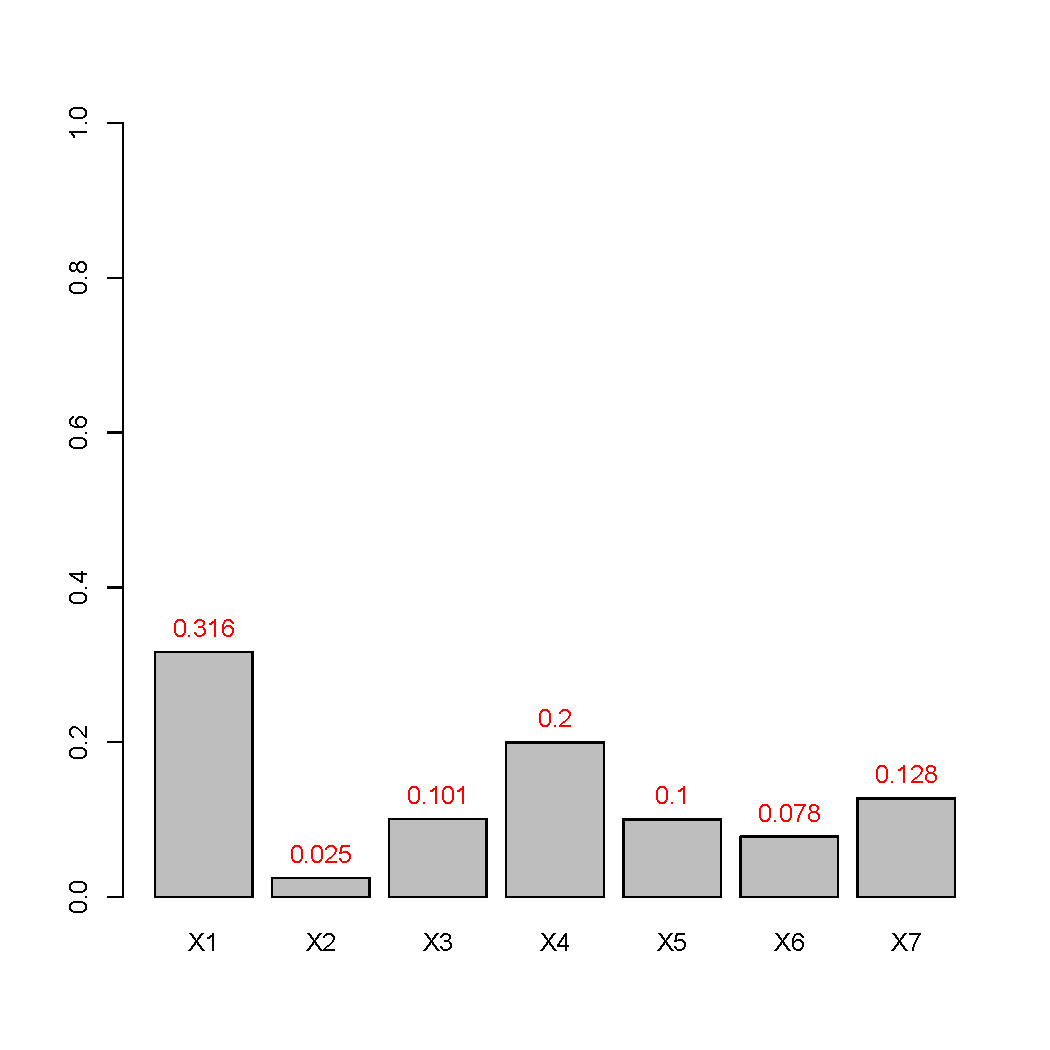
\includegraphics[scale=0.53]{Chapter2/Pictures/first_sobol.pdf}
    \caption{First-order Sobol indices}
\end{figure}

\begin{figure}
    \centering
    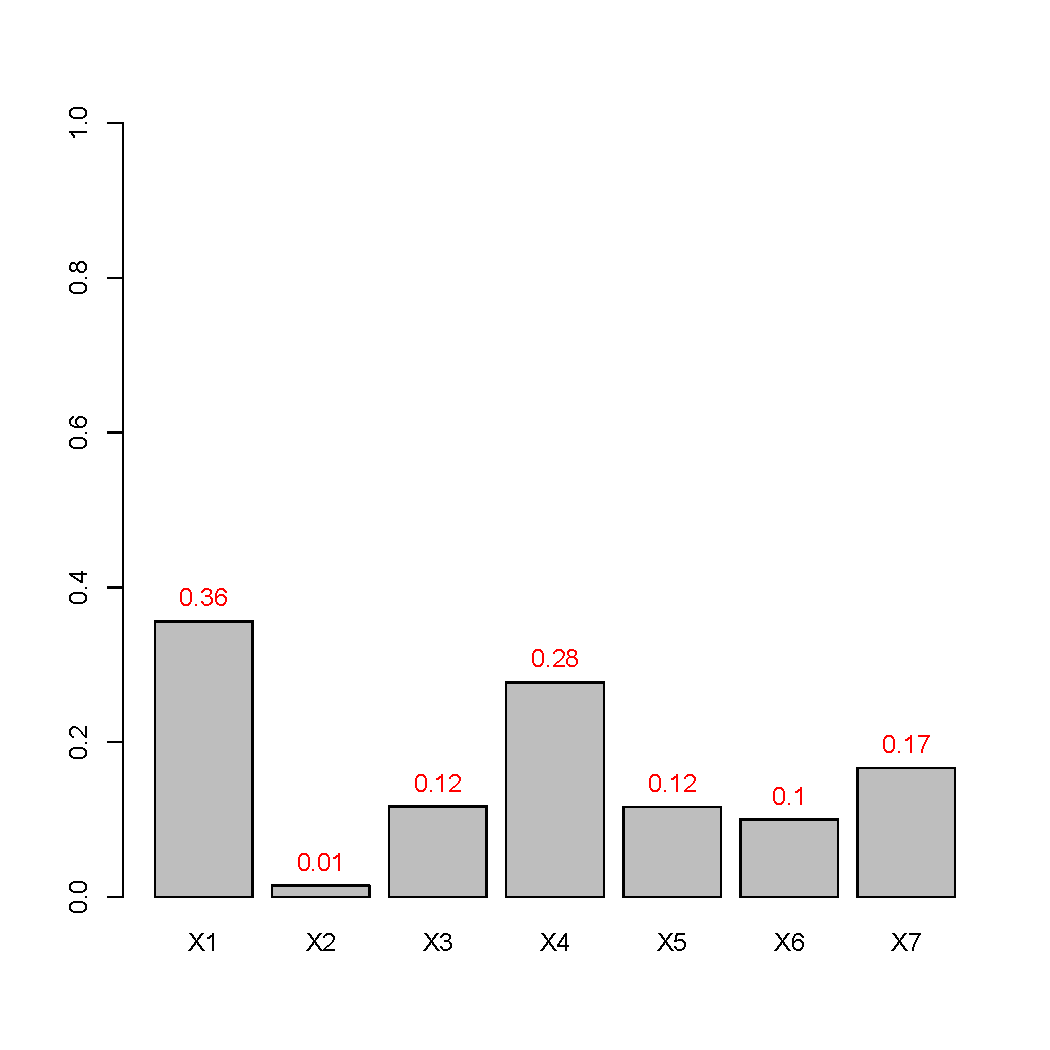
\includegraphics[scale=0.53]{Chapter2/Pictures/total_sobol.pdf}
    \caption{Total-order Sobol indices}
\end{figure}

The description of the parameters are as in  %\ref{tab:Parameters_range}.
\iffalse
\sout{follows, X1 - Thickness of the disc, X2 - Outer radius of the disc, X3 - Inner radius of the disc, X4 - Thickness of the pad, X5 - Inner radius of the pad, X6 - Outer radius of the pad and X7 - Angle of the pad.} 
\fi

As it can be seen, the first-order indices show relatively high values for the parameters X1 - thickness of the disc and X4 - thickness of the pad. The total-order indices also increase relatively for the two parameters. But the global variance of the stability criteria can be largely attributed to independent effects from the parameters rather than interaction between them. \\

Further, the results are also shown with closed second-order indices, combining the independent effects and the interaction between any two parameters.

\begin{figure}
    \centering
    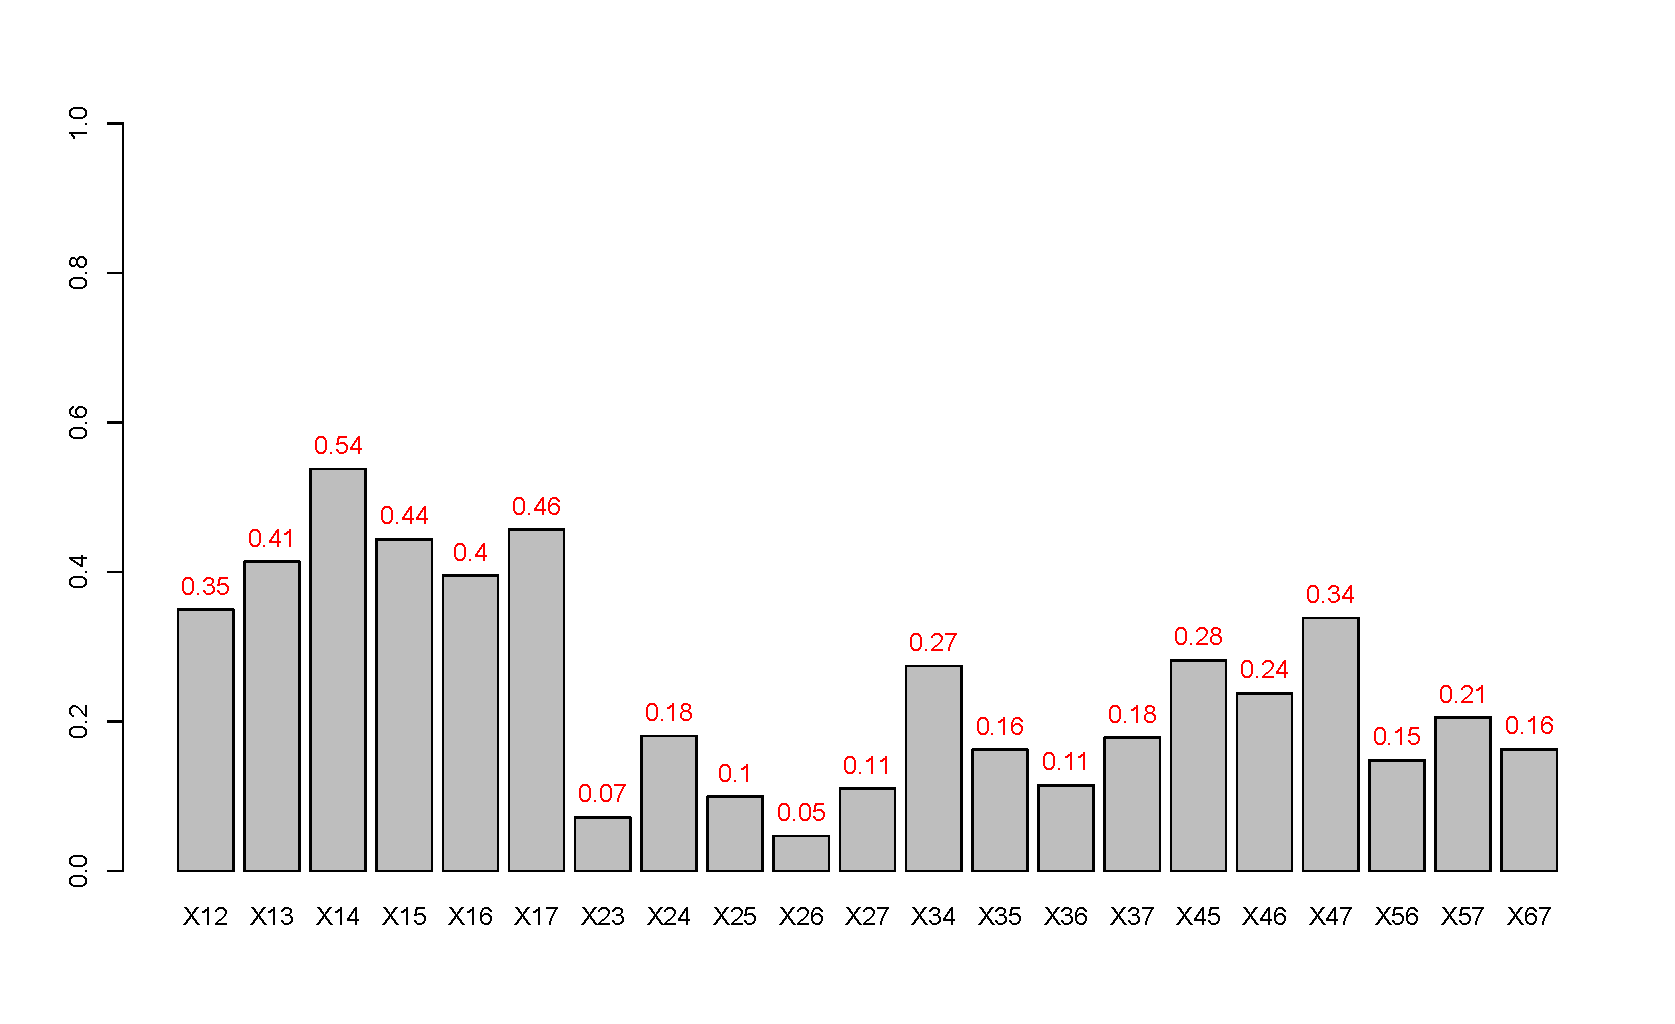
\includegraphics[scale=0.53]{Chapter2/Pictures/second_order_sobol.pdf}
    \caption{Closed second-order Sobol indices}
\end{figure}

\chapter{IGA based optimisation scheme}
%The way to build the optimization chain with metamodelisation Paper2

\subsection{IGA optimization setting}

In this section, we detail the shape optimization defined through NURBS parameterization of shapes for the pad, with its associated constraints and objectives for optimization. We also provide a short description of parameterization and refinement strategy for the disc-pad system domain $\Omega^{(\mathrm{d-p})}$.\\

The optimization is defined for the boundary $\partial \Gamma_{C}^{(\mathrm p)}$ of the planar surface $\Gamma_{C}^{(\mathrm p)}$ of the pad which is in contact with the disc, where the thickness of the pad and the design parameters of the disc are set to be constant. The geometry of $\Gamma_{C}^{(\mathrm{p})}$ can be parameterized through NURBS as

\begin{equation}
    \bm {\check{X}}_{s}^{(\mathrm p)}(\xi,\eta) = \sum_{i=0}^n \sum_{j=0}^m R_{i,p}(\xi)R_{j,q}(\eta)\bm{P}_{i,j}
\end{equation}

  Hence, in this setting, the shape optimization is defined for the shape of the NURBS curves $\bm X_{c}^{(1)}(s),\bm {\check{X}}_{c}^{(2)}(t),\bm {\check{X}}_{c}^{(3)}(u)$and $\bm X_{c}^{(4)}(v)$ which parameterizes $\partial \Gamma_{C}^{(\mathrm p)}$ that encloses the surface $\bm X_s^{(\mathrm p)}(\xi,\eta)$, as shown in Figure \ref{fig:Des_dom}, where the curves can be expressed as
  
  \begin{equation}\label{curves_bound}
    \begin{array}{lr}
    \bm {\check{X}}_{s}^{(\mathrm p)}(\xi,\eta|\xi=0)=\bm X_c^{(1)}(s)\\
    \bm {\check{X}}_{s}^{(\mathrm p)}(\xi,\eta|\eta=0)=\bm X_c^{(2)}(t)\\
    \bm {\check{X}}_{s}^{(\mathrm p)}(\xi,\eta|\xi=1)=\bm X_c^{(3)}(u)\\
    \bm {\check{X}}_{s}^{(\mathrm p)}(\xi,\eta|\eta=1)=\bm X_c^{(4)}(v)
    \end{array}
\end{equation}

\begin{figure}[h!]
    \centering
    \includegraphics[scale=0.3]{Chapter5/Pictures/des_dom.pdf}
    \caption{An illustration describing the parameterisation of $\Gamma_{c_{Pad}}$ and $\partial \Gamma_{c_{Pad}}.$  }
    \label{fig:Des_dom}
\end{figure}

This leads to the problem of defining the parameterisation $ \bm {\check{X}}_{s}^{(\mathrm p)}(\xi,\eta)$ given the four parametric curves $\bm X_c^{(1)}(s),\bm X_c^{(2)}(t),\bm X_c^{(3)}(u)$ and $\bm X_c^{(4)}(v)$.  The parameterisation should be characterized by injective mapping which is ensured if the Jacobian does not vanish. For $\bm X: \hat{\Omega}\rightarrow \Omega$, verifying Jacobian on $\hat{\Omega}$ in transfinite sense would be impossible, for which it can be verified in a finite sense with the property of determinant-Jacobian function for a NURBS parameterisation. The definition of determinant of Jacobian for a NURBS parameterisation can be expressed as a function of higher-order NURBS to the NURBS parameterisation, given as

\begin{equation}
|\bm J( \bm {\check{X}}_{s}(\xi,\eta) )|= \big|\begin{bmatrix}\frac{\partial \bm X_s}{\partial \xi} & \frac{\partial \bm X_s}{\partial \eta}\end{bmatrix}\big|= \sum_{i=1}^{2n-1}\sum_{j=1}^{2m-1}   R_{i,2p-1}(\xi)R_{j,2q-1}(\eta)\bm{O}_{i,j}
\end{equation}

The condition for injective mapping $|\bm J( \bm {\check{X}}_{s}(\xi,\eta) )|>0$ for $(\xi,\eta) \in [0,1]^2$ can be said to be satisfied if $\bm{O}_{i,j}>0$, which is  a sufficient condition but not a necessary one. This is because, if $|\bm J( \bm {\check{X}}_{s}(\xi,\eta) )|=0$ for any point on boundary, even though $|\bm J( \bm {\check{X}}_{s}(\xi,\eta) )|>0$ on $(0,1)^2$,  $\bm{O}_{i,j}<0$. Nevertheless, $\bm{O}_{i,j}$ is often considered to check the validity of a  parameterisation for injectivity, especially in the scope of defining optimisation to achieve an injective parameterisation.\\
 
The general idea behind Isogeometric approach is that given an initial parameterisation $\breve{\bm X}$ of a domain $\Omega$ with NURBS, analysis-suitable parameterisation $\bm X$ can be achieved with in the same parametric space, through addition or manipulation of knots and control points. But achieving initial parameterisation with injective mapping can be a difficult challenge especially for arbitrary definition of shapes in an optimisation, where to achieve a quality parameterisation with injective mapping can be even more challenging. The problem of defining $\breve{\bm X}$ is more related to computer-aided design (CAD), where the role of CAD is typically not focused on defining $\bm X$. This is because, for the illustration of CAD, there can be multiple ways to parametrise a domain, that may not necessarily be suited for defining an approximation space ${}_h \bm V$ in the context of isogeometric analysis as $\bm \Phi$ \footnote{To distinguish the space ${}_h \bm V$ in the context of isogeometric approach, we define $\bm \Phi$ to be ${}_h \bm V$}. A typical approach in CAD is that a complicated domain being defined as a trimmed domain\footnote{The definition of $\Omega$ as a trimmed domain can be defined as $\Omega \subset \Omega_{\uplus}$, where $\hat{\Omega}\rightarrow\Omega_{\uplus}$ } (Fig. \ref{fig:trimmed_dom}) or union of several trimmed domains. 

\begin{figure}[h!]
    \centering
    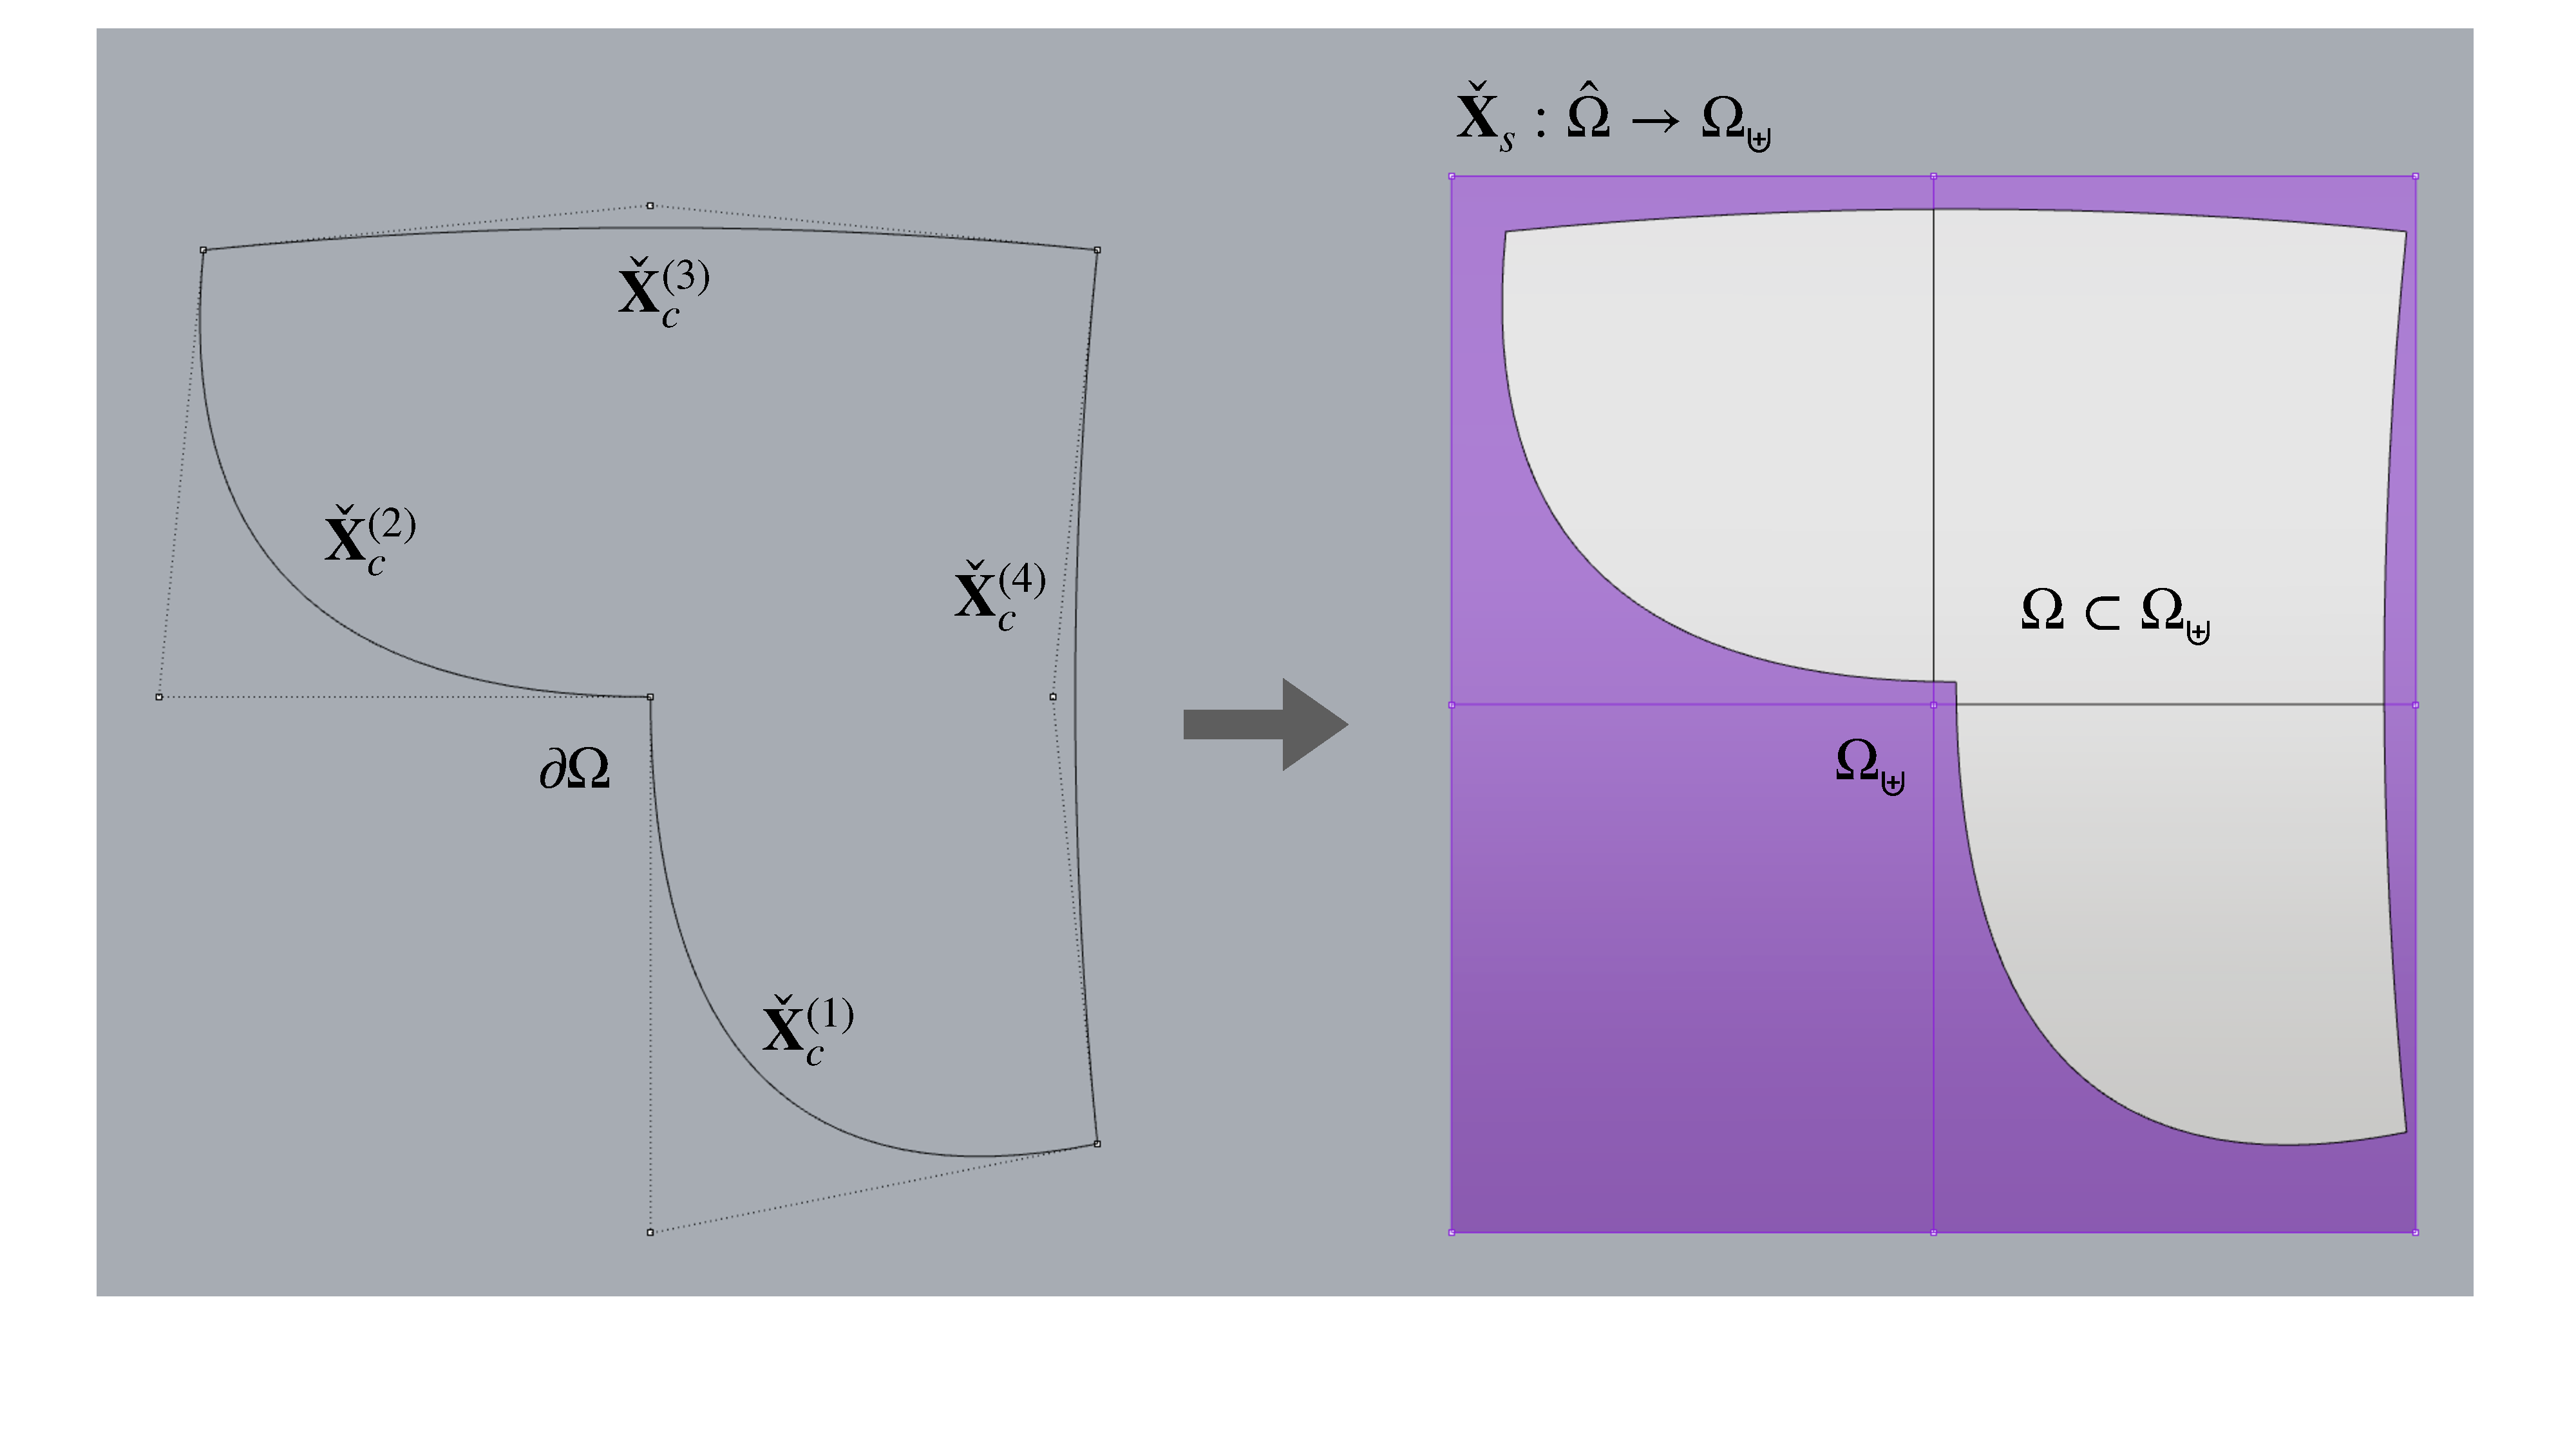
\includegraphics[scale=0.25]{Chapter5/Pictures/trimmed_dom}
    \caption{Parameterisation with trimmed domain }
    \label{fig:trimmed_dom}
\end{figure}


For the definition of a trimmed domain, since only essential part of the mapping that defines the domain from the parametric space to the physical space is considered, it does not place severe restriction over the complete parametric space to be mapped to the domain, illustrated in. This can be better in the context of designing where a surface can be loosely defined to contain a closed curve, but may not be suitable for defining $\bm \Phi$. One could say that for $\Omega \subset \Omega_{\uplus}$, with $\Omega_{\uplus}$ parameterised by $\bm X$, and given the bases $\bm \phi_\mathrm{i}:= \bm R_{i,j,k}(\mathbf{\Xi}) \circ \bm{X}^{-1}$, only the bases $\bm \phi_\mathrm{i}$ defining $\Omega$ can be considered for approximation. 
This is essentially the approach of the immersed methods, where typically the bases $\bm \phi_\mathrm{i}$ defining $\Omega$ is distinguished with material properties at the quadrature points, along with local refinement at the boundary of $\Omega\subset\Omega_{\uplus}$ through hierarchical refinement. Though immersed methods can have more flexibility in defining ${}_h \bm V$, we do not focus on such approaches owing to its novelty which can require immense time to develop.
 We purely focus on defining $\bm X:\hat\Omega\rightarrow\Omega$ which can be called body-fitted parameterisation. 
 The point is that to achieve body-fitted injective parameterisation for any shape as initial parameterisation can be too demanding from purely the perspective of CAD (Fig. (Fig. \ref{fig:body_neg}). 
 
 \begin{figure}[h!]
    \centering
    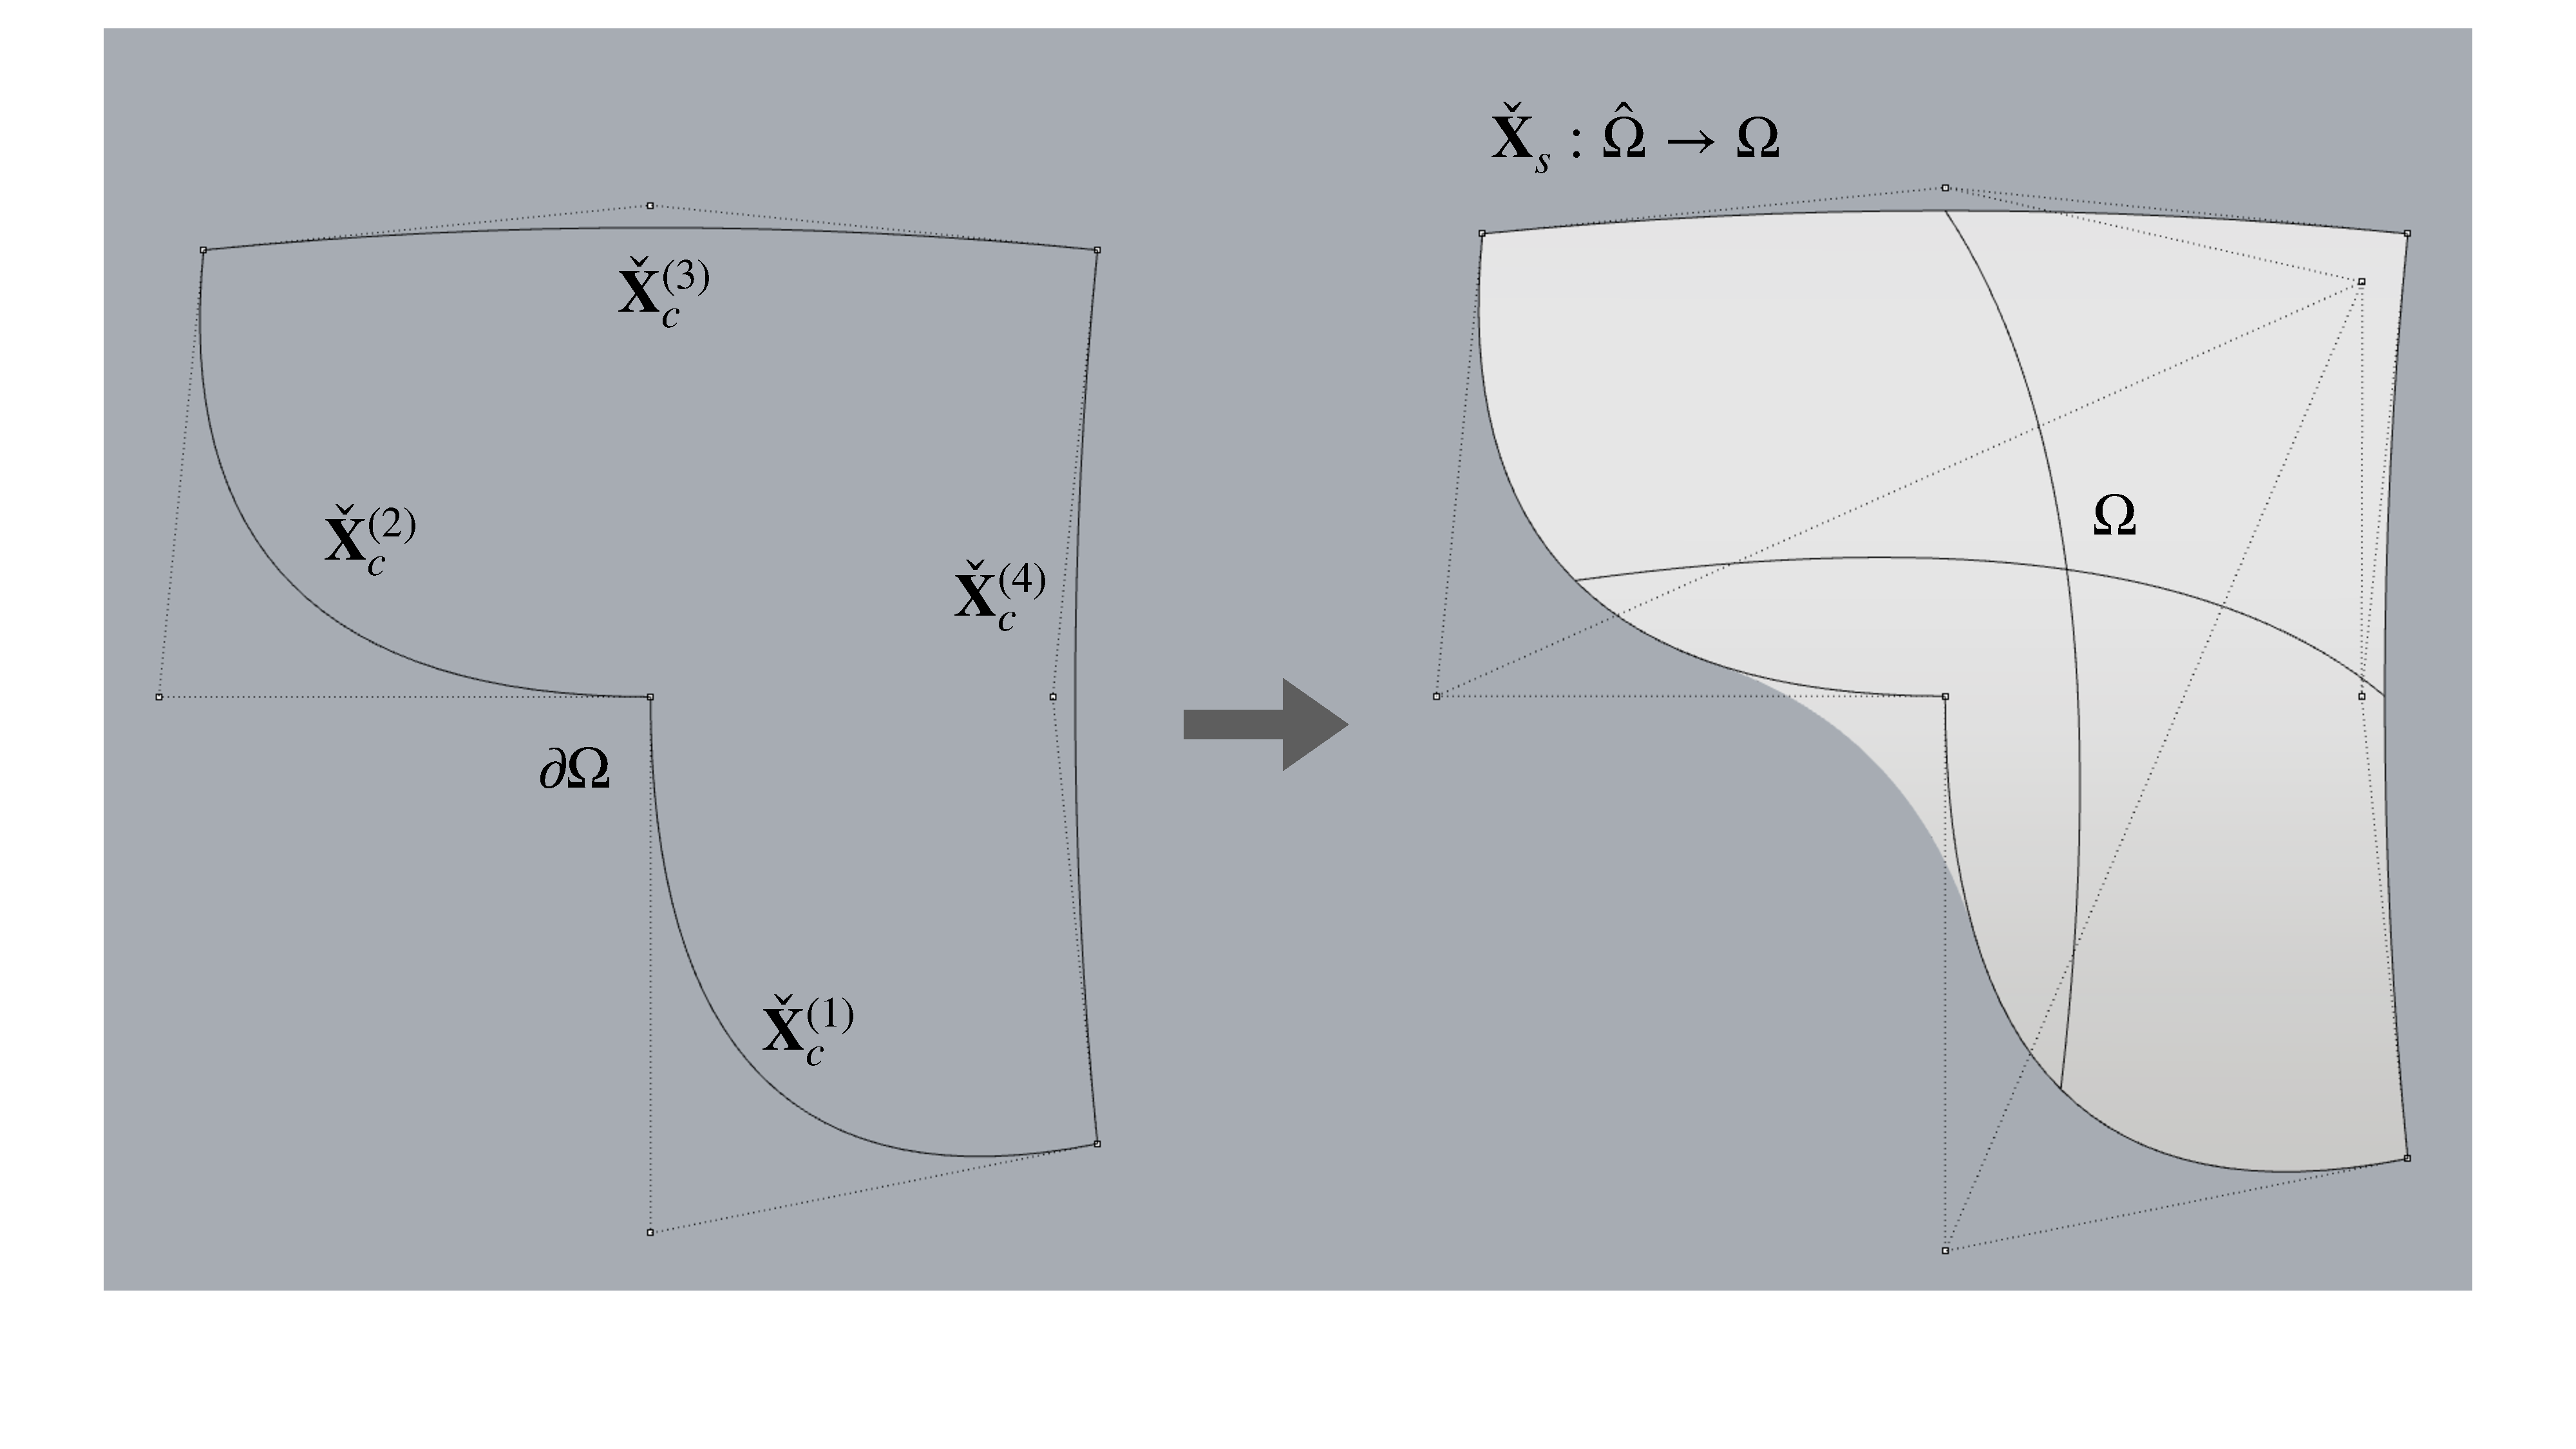
\includegraphics[scale=0.25]{Chapter5/Pictures/body_neg}
    \caption{Body-fitted non-injective parameterisation }
    \label{fig:body_neg}
\end{figure}


%Typically, the boundary of a domain is parametrised with lesser control points as parameters to define shapes, where to achieve an initial parameterisation given the boundary parameterisation can be sometimes impossible with lesser control points. 
For complex shapes, it is typically preferred to define analysis-suitable parameterisation directly, rather from a prior definition of initial parameterisation, where analysis-suitable parameterisation with sufficient refinement can be well suited to define injective parameterisation. 
From the perspective of CAD, this makes no difference as along as body-fitted injective parameterisation is achieved and hence, sometimes, no distinguish can necessarily be made between initial and analysis-suitable parameterisations (Fig. \ref{fig:body_pos}). 

 \begin{figure}[h!]
    \centering
    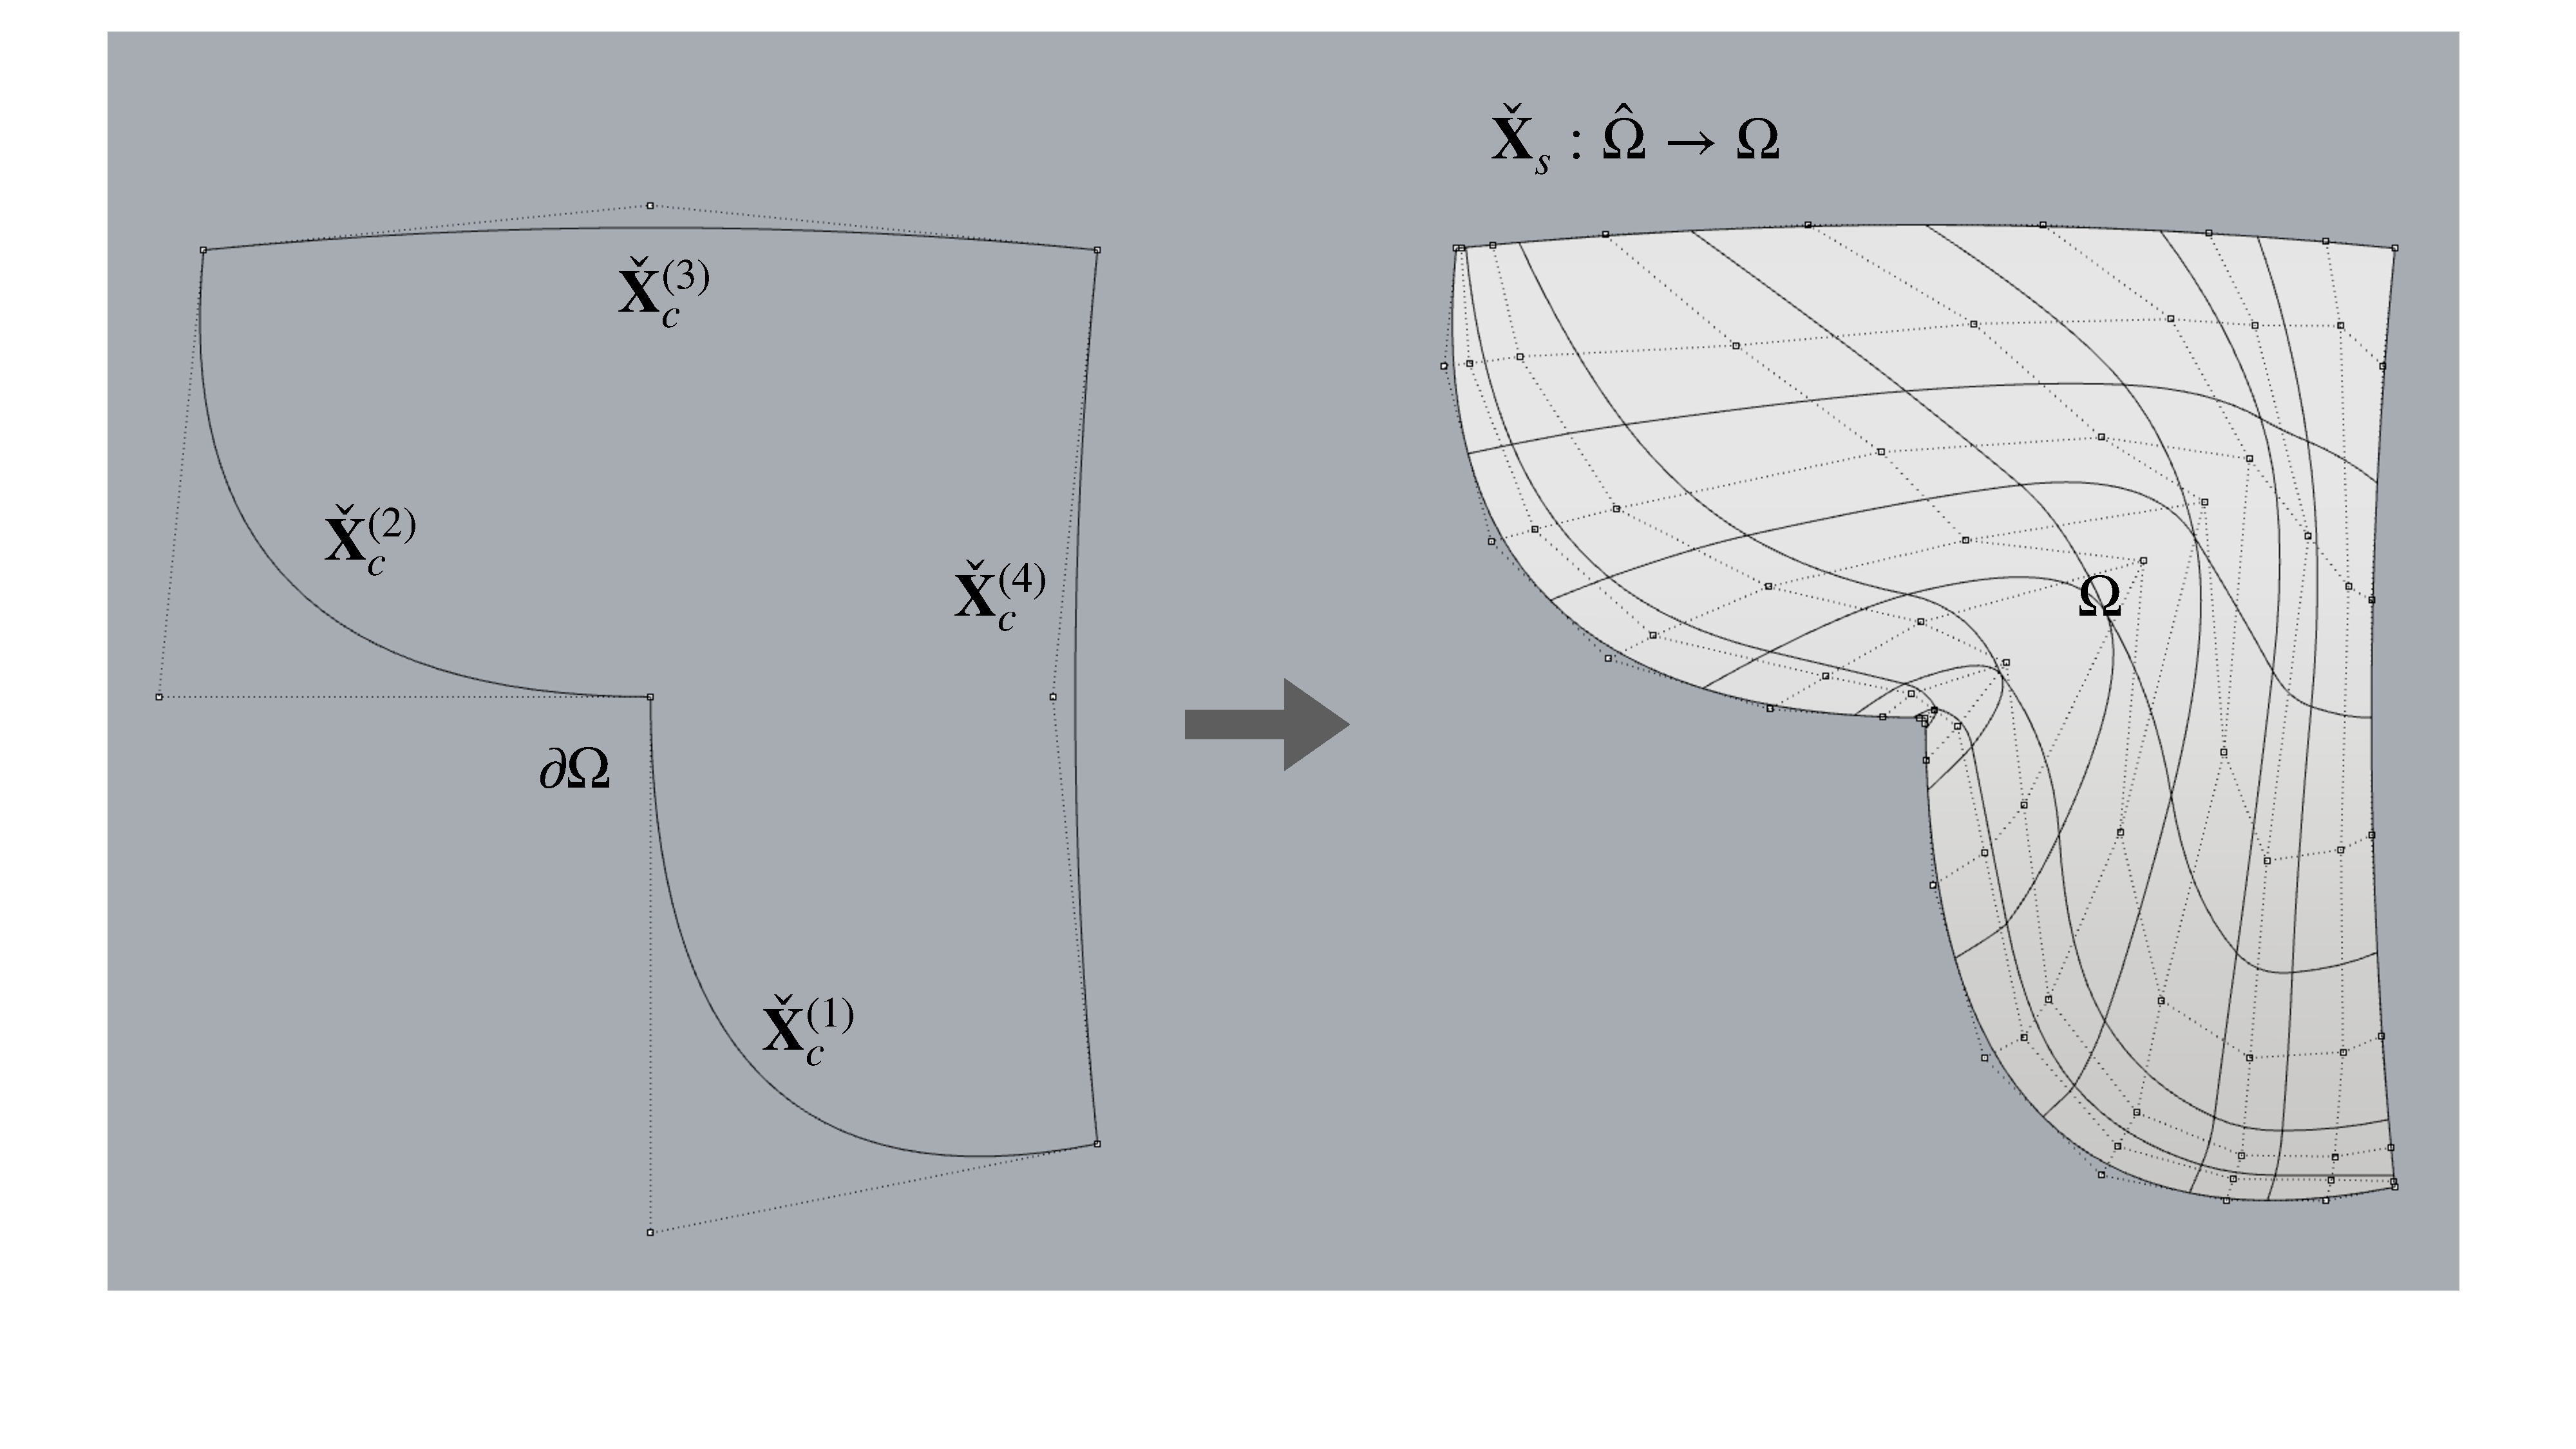
\includegraphics[scale=0.25]{Chapter5/Pictures/body_pos}
    \caption{Body-fitted injective parameterisation}
    \label{fig:body_pos}
\end{figure}

%At least for the definition of the boundary, we must talk about initial parameterization, in our case, with the chosen approach for parameterisation, for all parameterisation %Hence, expecting an initial parameterisation as body-fitted parameterisation for CAD can be very demanding, since for more complicated shapes it typically requires non-linear optimisation to find an injective body-fitted parameterisation.
%We stick with the narration of defining initial parameterisation prior to analysis-suitable parameterisation, since with the considered definition of shapes, it is possible to distinguish initial and analysis-suitable parameterisations, through there may not be an explicit advantage of this narration in our case.
Nevertheless, given the complexity of defining initial or analysis-suitable parameterisation, it is seen as a more robust strategy to define ${}_h \bm V$ compared to classical FEM. 
It should also be reminded that a complex domain can also be defined through multiple patches, where each patch corresponds to body-fitted parameterisation. But this also requires a more robust strategy to split a complex domain in to patches for any arbitrary definition of shape, at least for a fixed topology.
Nevertheless, we adapt multi-patch parameterisation as a strategy for local refinement and sub-structuring in optimisation.\\

For the scope of this thesis, we consider discrete Coon's patch method as a preliminary approach for the parameterisation part of the Bayesian shape optimisation framework. The idea is to adapt a more advanced parameterisation strategy for future evolution of the framework.\\



The parameterization of$ \bm {\check{X}}_{s}^{(\mathrm p)}(\xi,\eta)$ with the above four curves \eqref{curves_bound} by discrete Coon's patch method can be given as

\begin{multline}
    \bm {\check{X}}_{s}^{(\mathrm p)}(\xi,\eta) =\bm {\check{X}}_{c}^{(1)}(s)(1-\xi)+\bm X_c^{(3)}(u)(\xi)+\bm {\check{X}}_{c}^{(2)}(t)(1-\eta)+\bm X_c^{(4)}(v)(\eta)\\-\bm {\check{X}}_{c}^{(1)}(0)(1-\xi)(1-\eta) - \bm  X_c^{(1)}(1)(1-\xi)(\eta)\\ -\bm {\check{X}}_{c}^{(3)}(0)(\xi)(1-\eta) -\bm {\check{X}}_{c}^{(3)}(1)(\xi)(\eta)
\end{multline}

where the Coon's patch method is an explicit linear method and hence computationally efficient in realising parameterisation, but the method doesn't guarantee injective mapping. 
In our experience, the shapes realised through Coon's patch method that doesn't satisfy injective mapping are largely too conceptual for pad shapes and hence, given the complexity of realising parameterisation for such shapes, we only stick with the shapes realised through Coon's patch method for which injective property is satisfied.\\

In the scope of shape optimisation,$ \bm {\check{X}}_{s}^{(\mathrm p)}(\xi,\eta)$ can be defined as the function to be optimised, on which constraints can be imposed.
We define Constraint set 1, which contains constraints intrinsic of the boundary curves \eqref{curves_bound}. For simplicity owing to the preliminary definition of framework, in order to limit the parameters in optimization, we restricted the degree of each curve to $2$ and hence, this leads to the surface$ \bm {\check{X}}_{s}^{(\mathrm p)}(\xi,\eta)$ with the property $p=q=2$, and each curve is defined only through three control points which are just enough to define a curve of degree $2$. 
Furthermore, the optimisation is defined only for the position of the control points $\bm{P}_{i,j}$ for $w_{i,j} =1$ \eqref{NURBS_c}, i.e, we considered the optimization of the NURBS geometry only through affine transformation without considering projective transformation.\\
 
While the end control points will be constrained relative to the disc domain, given in Constraint set 3, we impose constraint on the mid-control point of each curve segment. The control points for any curve segment can be expressed as $\bm P_1$, $\bm P_2$ and $\bm P_3$, where $\bm P_1$ and $\bm P_3$ define the end control points. If the initial configuration of the curve can be expressed as a line segment $\overline{\bm P_1\bm P_3}$ with $\bm P_2 = \frac{\bm P_1+\bm P_3}{2}$, then the constraint on $\bm P_2$ can be expressed relative to the initial configuration as $\bm P_2 \perp \overline{\bm P_1\bm P_3}$\\


Constraints between curve segments are given as Constraint set 2 which contains constraints to confirm injective mapping, which also implicitly preserves topology.
Injective parameterisation can be said to be achieved if $ |\bm J( \bm {\check{X}}_{s}(\xi,\eta) )|$ does not vanish on all $\hat{\Omega}$.
With the mid-control points constrained, the set of constraints for testing this condition was realised geometrically, given as\\
 
{
Constraint set 2: 
\begin{multline}
   \quad \{\bm X_c^{(1)}(s) \cap\bm {\check{X}}_{c}^{(2)}(t)\}\cup \{\bm X_c^{(3)}(u) \cap\bm {\check{X}}_{c}^{(4)}(v)\}\cup \{\bm X_c^{(1)}(s) \cap\bm {\check{X}}_{c}^{(3)}(u)\}\cup\\
   \{\bm X_c^{(1)}(s) \cap\bm {\check{X}}_{c}^{(4)}(v)\} \cup \{\bm X_c^{(2)}(t) \cap\bm {\check{X}}_{c}^{(3)}(u)\} \cup \{\bm X_c^{(2)}(t) \cap\bm {\check{X}}_{c}^{(4)}(v)\} = \emptyset\\ 
\forall s,t,u,v \in (0,1)\\
\\
\{\bm X_c^{(1)}(0)(1-\xi)+\bm X_c^{(3)}(0)(\xi)\} \cap \{\bm X_c^{(1)}(0+\Delta s)(1-\xi)+\bm X_c^{(3)}(0+\Delta u)(\xi)\} = \emptyset\\
\{\bm X_c^{(1)}(1)(1-\xi)+\bm X_c^{(3)}(1)(\xi)\} \cap \{\bm X_c^{(1)}(1-\Delta s)(1-\xi)+\bm X_c^{(3)}(1-\Delta u)(\xi)\} = \emptyset\\
\{\bm X_c^{(2)}(0)(1-\eta)+\bm X_c^{(4)}(0)(\eta)\} \cap \{\bm X_c^{(2)}(0+\Delta t)(1-\eta)+\bm X_c^{(4)}(0+\Delta v)(\eta)\} = \emptyset\\
\{\bm X_c^{(2)}(1)(1-\eta)+\bm X_c^{(4)}(1)(\eta)\} \cap \{\bm X_c^{(2)}(1-\Delta t)(1-\eta)+\bm X_c^{(4)}(1-\Delta v)(\eta)\} = \emptyset\\
\forall \xi,\eta \in [0,1]
\end{multline}
}
where $\Delta$ represents an arbitrary small variation. The first constraint avoids intersection between the curves except for the end points. Satisfying the first constraint which guarantees a fixed topology does not assure injective parameterisation through Coon's patch method, for which the last set of four constraints are necessary.  The last set of four constraints implicitly avoid concave intersection between the curves. Given that the curves do not intersect except for convex intersection at the end points, and with constraints on the mid-control points, injective parameterisation can be achieved with Coon's patch method. \\
% Alternate way to realise

Further, the definition of the pad surface to be with in the bounds of the disc surface is given through a box constraint as follows\\

Constraint set 3: \\
\begin{equation}
    (\bm X_{s(lb)} \leq \bm X_s^{(\mathrm p)}(\xi,\eta) \leq \bm X_{s(ub)}) :   \{[\bm X_{c(lb)}^{(i)},\bm X_{c(ub)}^{(i)}]\} \cap   \{[\bm X_{c(lb)}^{(j)},\bm X_{c(ub)}^{(j)}]\} = \emptyset  
\end{equation}

where the choice of $\bm X_{s(lb)}$ and $\bm X_{s(ub)}$ depends on the design choice for the domain of the disc to be in contact with the pad. Further, the box constraint is adapted to limit the redundancies in geometric description i.e, to limit the scope for a given shape to be defined in more than one way with in the same design space. To avoid this type of redundancy, we restricted the domain through box constraints for at least two curves $\bm X_{c}^{(i)}(.)$ and $\bm X_{c}^{(j)}(.)$ of the four curves, such that the intersection of their domains is a null set. This leads to restriction of the design space with compromise on reducing the redundancies. Hence, we avoided some of the redundancies on empirical notion, such that the restricted design space has lesser meaningful designs. This maybe an interesting anomaly to investigate, since the redundancies may lead to larger design space with more severe multi-modality.\\   

We further impose an inequality constraint in order to avoid designs with smaller contact surface, given as\\

Constraint 4: \\
\begin{equation}
    Area(\bm X_{s}^{(\mathrm p)}(\xi,\eta)) \geq A_{min}
\end{equation}

where $Area(\bm X_{s}^{(\mathrm p)}(\xi,\eta)): \int_{\xi}\int_{\eta}|\frac{\partial \bm {\check{X}}_{s}^{(\mathrm p)}}{\partial \xi} \times \frac{\partial \bm {\check{X}}_{s}^{(\mathrm p)}}{\partial \eta}|d\xi d\eta$ and the choice of $A_{min}$ depends on the minimum contact surface area that is required on the Pareto-front, since maximization of $Area(\bm X_{s}^{(\mathrm p)}(\xi,\eta))$ is defined to be one of the objectives.\\

The definition of the shape of$ \bm {\check{X}}_{s}^{(\mathrm p)}(\xi,\eta)$ through this strategy means that there is no requisite for a reference configuration to define optimization, but instead the pad shapes are defined through random generation of curves with $C^0$ continuity between them. We assume that this restricts bias to any specific shape and hence encouraging more randomness in defining a meaningful geometry. 
This highly restricts the use of gradient-based approaches for optimization, since the constraints are also black-box and may have discontinuities. 
Some of the limitations can also be attributed to lack of exploring classical shapes such as the annulus sector pad shapes in our application even though such shapes are already a subset of the the design space defined. The randomness in the definition of shapes can lead to higher probability of failure for the constraints, and hence more constraint evaluation in optimisation.\\

Finally, the objectives for the Multi-objective optimization can be posed as optimization of the following functionals: 

\begin{itemize}
    \item Objective 1:
$min \, C_{\mathsf s}(\bm X_{s}^{(\mathrm p)}(\xi,\eta)\,|\,\Im(\bm \Lambda(\bm X^{(\mathrm{d-p})})\in[10KHz,13KHz])$
    \item Objective 2:
$max \, Area(\bm X_{s}^{(\mathrm p)}(\xi,\eta))$
\end{itemize}

%Objective 1:
%$min \, C_s(\bm X_{s}^{(\mathrm p)}(\xi,\eta))\,|\,\Im(\Lambda(\bm X_{s}^{(\mathrm p)}(\xi,\eta)))\in[10KHz,13KHz]$

%Objective 2: 
%$max \, Area(\bm X_{s}^{(\mathrm p)}(\xi,\eta))$

where the optimisation of the functionals are defined over the space of NURBS functions. Since we fixed the order and the number of control points of the NURBS surface$ \bm {\check{X}}_{s}^{(\mathrm p)}(\xi,\eta)$, the optimisation is restricted to a fixed number of control points.\\ 

\subsection{Isogeometric parameterization and refinement strategies for the disc-pad system domain with contact considerations} \label{subsec:iso_ref_strat}
{For the following, we do not focus on the mesh sensitivity for CEA or the stability criterion $C_{\mathsf s}$, but instead the below refinement strategies can be seen as to realise the classical mesh refinement considerations for a contact problem, where more elements are typically defined on $\Gamma_C$ and at the vicinity of $\partial \Gamma_C$ to capture more accurately the contact characteristics and the strong solution gradient. This is especially more challenging with local refinement for NURBS parameterization, hence we expose here some strategies to achieve local refinement. Empirically, the refinement at $\Gamma_C$ and around $\partial \Gamma_C$ seems to effect the results of CEA and converges with sufficient refinement, but a more qualitative assessment of the sensitivity has not been developed here, since it requires a detailed study of not only the refinement but also the contact formulation and  the nature of modelling contact stiffness.}\\

The planar parameterization$ \bm {\check{X}}_{s}^{(\mathrm p)}$ can be easily extended to define $\Omega^{(\mathrm p)}$ as $\bm X_{v}^{(\mathrm p)}$ considering the thickness of the pad through the tensor product definition \eqref{NURBS_v}, given a NURBS line along the thickness. 
The disc domain $\Omega^{(\mathrm d)}$ was realised by multi-patch parameterization $\bm X_{v}^{(\mathrm d)} := \bm X_{v}^{(\mathrm d_1)} \cup \bm X_{v}^{(\mathrm d_2)}$ to achieve local refinement on $\Gamma_C^{(\mathrm d_2)}$. {The surface parameterization for the disc patches$ \bm {\check{X}}_{s}^{(\mathrm d_1)}$ and$ \bm {\check{X}}_{s}^{(\mathrm d_1)}$ can be achieved through the concept of revolved surface, detailed in \citep{Piegl1995TheNB}, which assures robust injective parameterisation since the curve to be revolved is a straight line perpendicular to the disc axis, given that the straight line does not pass through the axis. The planar parameterizations$ \bm {\check{X}}_{s}^{(\mathrm d_1)}$ and$ \bm {\check{X}}_{s}^{(\mathrm d_2)}$ can be extended to $\bm X_{v}^{(\mathrm d_1)}$ and $\bm X_{v}^{(\mathrm d_2)}$ respectively, similar to achieving $\bm X_{v}^{(\mathrm p)}$}.\\

For any refinement, the space for parameterisation remains the same i.e, $(\xi,\eta,\zeta) \in [0,1]^3$ and the refinement is defined only through manipulation or addition of knots and control point to achieve an analysis-suitable parameterisation. 
After an analysis-suitable parameterisation, to take in to account of the additional control points and the manipulated knot vectors, $\bm X_{v}^{(\mathrm p)}$ and $\bm X_{v}^{(\mathrm d)}$ can be expressed as $\overline{X}_{v}^{(\mathrm p)}$ and $\overline{X}_{v}^{(\mathrm d)}$. 
Hence, the NURBS bases associated with $\overline{X}_{v}^{(\mathrm p)}$ and $\overline{X}_{v}^{(\mathrm d)}$ are used to define the space for approximation in isogeometric approach, detailed in Section \ref{cont_des}. It should be noted that often analysis-suitable parameterisation is achieved directly in the scope of defining an injective parameterisation, since for complex shapes, analysis-suitable parameterisation with sufficient refinement can be well suited to define injective parameterisation.
Hence, often no distinguish can be made between initial and analysis-suitable parameterisations, since the definition of body-fitted initial parameterisation in the context of CAD may already demand sufficient refinement to achieve even an elementary injective  parameterisation. Since we only choose designs for which injective parameterisation exists with Coon's patch method, it is safe to say that for any analysis-suitable injective parameterisation achieved through Coon's patch method, initial injective parameterisation can also be achieved by Coon's patch method. Hence, we talk in the context that initial parameterisation of CAD does not have sufficient refinement  to define the space ${}_h\bm V$ and hence we explicitly define analysis-suitable parameterisation through refinement.\\

%In the following, we show the strategy adapted to achieve  analysis-suitable parameterizations $\overline{X}_{v}^{Pad}$ and $\overline{X}_{v}^{Disc}$ in shape optimization.
 Normally across the boundary $\partial\Gamma_C$ of a contact domain $\Gamma_C$, there is drastic change in the solution gradient and hence, the parameterization needs special attention owing to the continuity of the NURBS bases. The tensor product property of the NURBS gives further challenge for local refinement which is usually desired on $\Gamma_C$. These challenges can be largely overcome by adaptation of NURBS bases to T-splines \citep{BAZILEVS2010229} or THB-splines \citep{GIANNELLI2012485}, but requires extensive adaptation. Hence, we defined a multi-patch parameterization strategy through collocation and projection of  properties defined on control points between two merging surfaces, which was simple and efficient for our application with fewer adaptation. Even though the considered multi-patch approach only considers $C^0$ solution continuity between the patches, the post-processing of the mode shapes show sufficient smoothness in displacement field across the patches, shown in Figure \ref{fig:MP_anatom}.\\

\begin{figure}[h!]
    \centering
    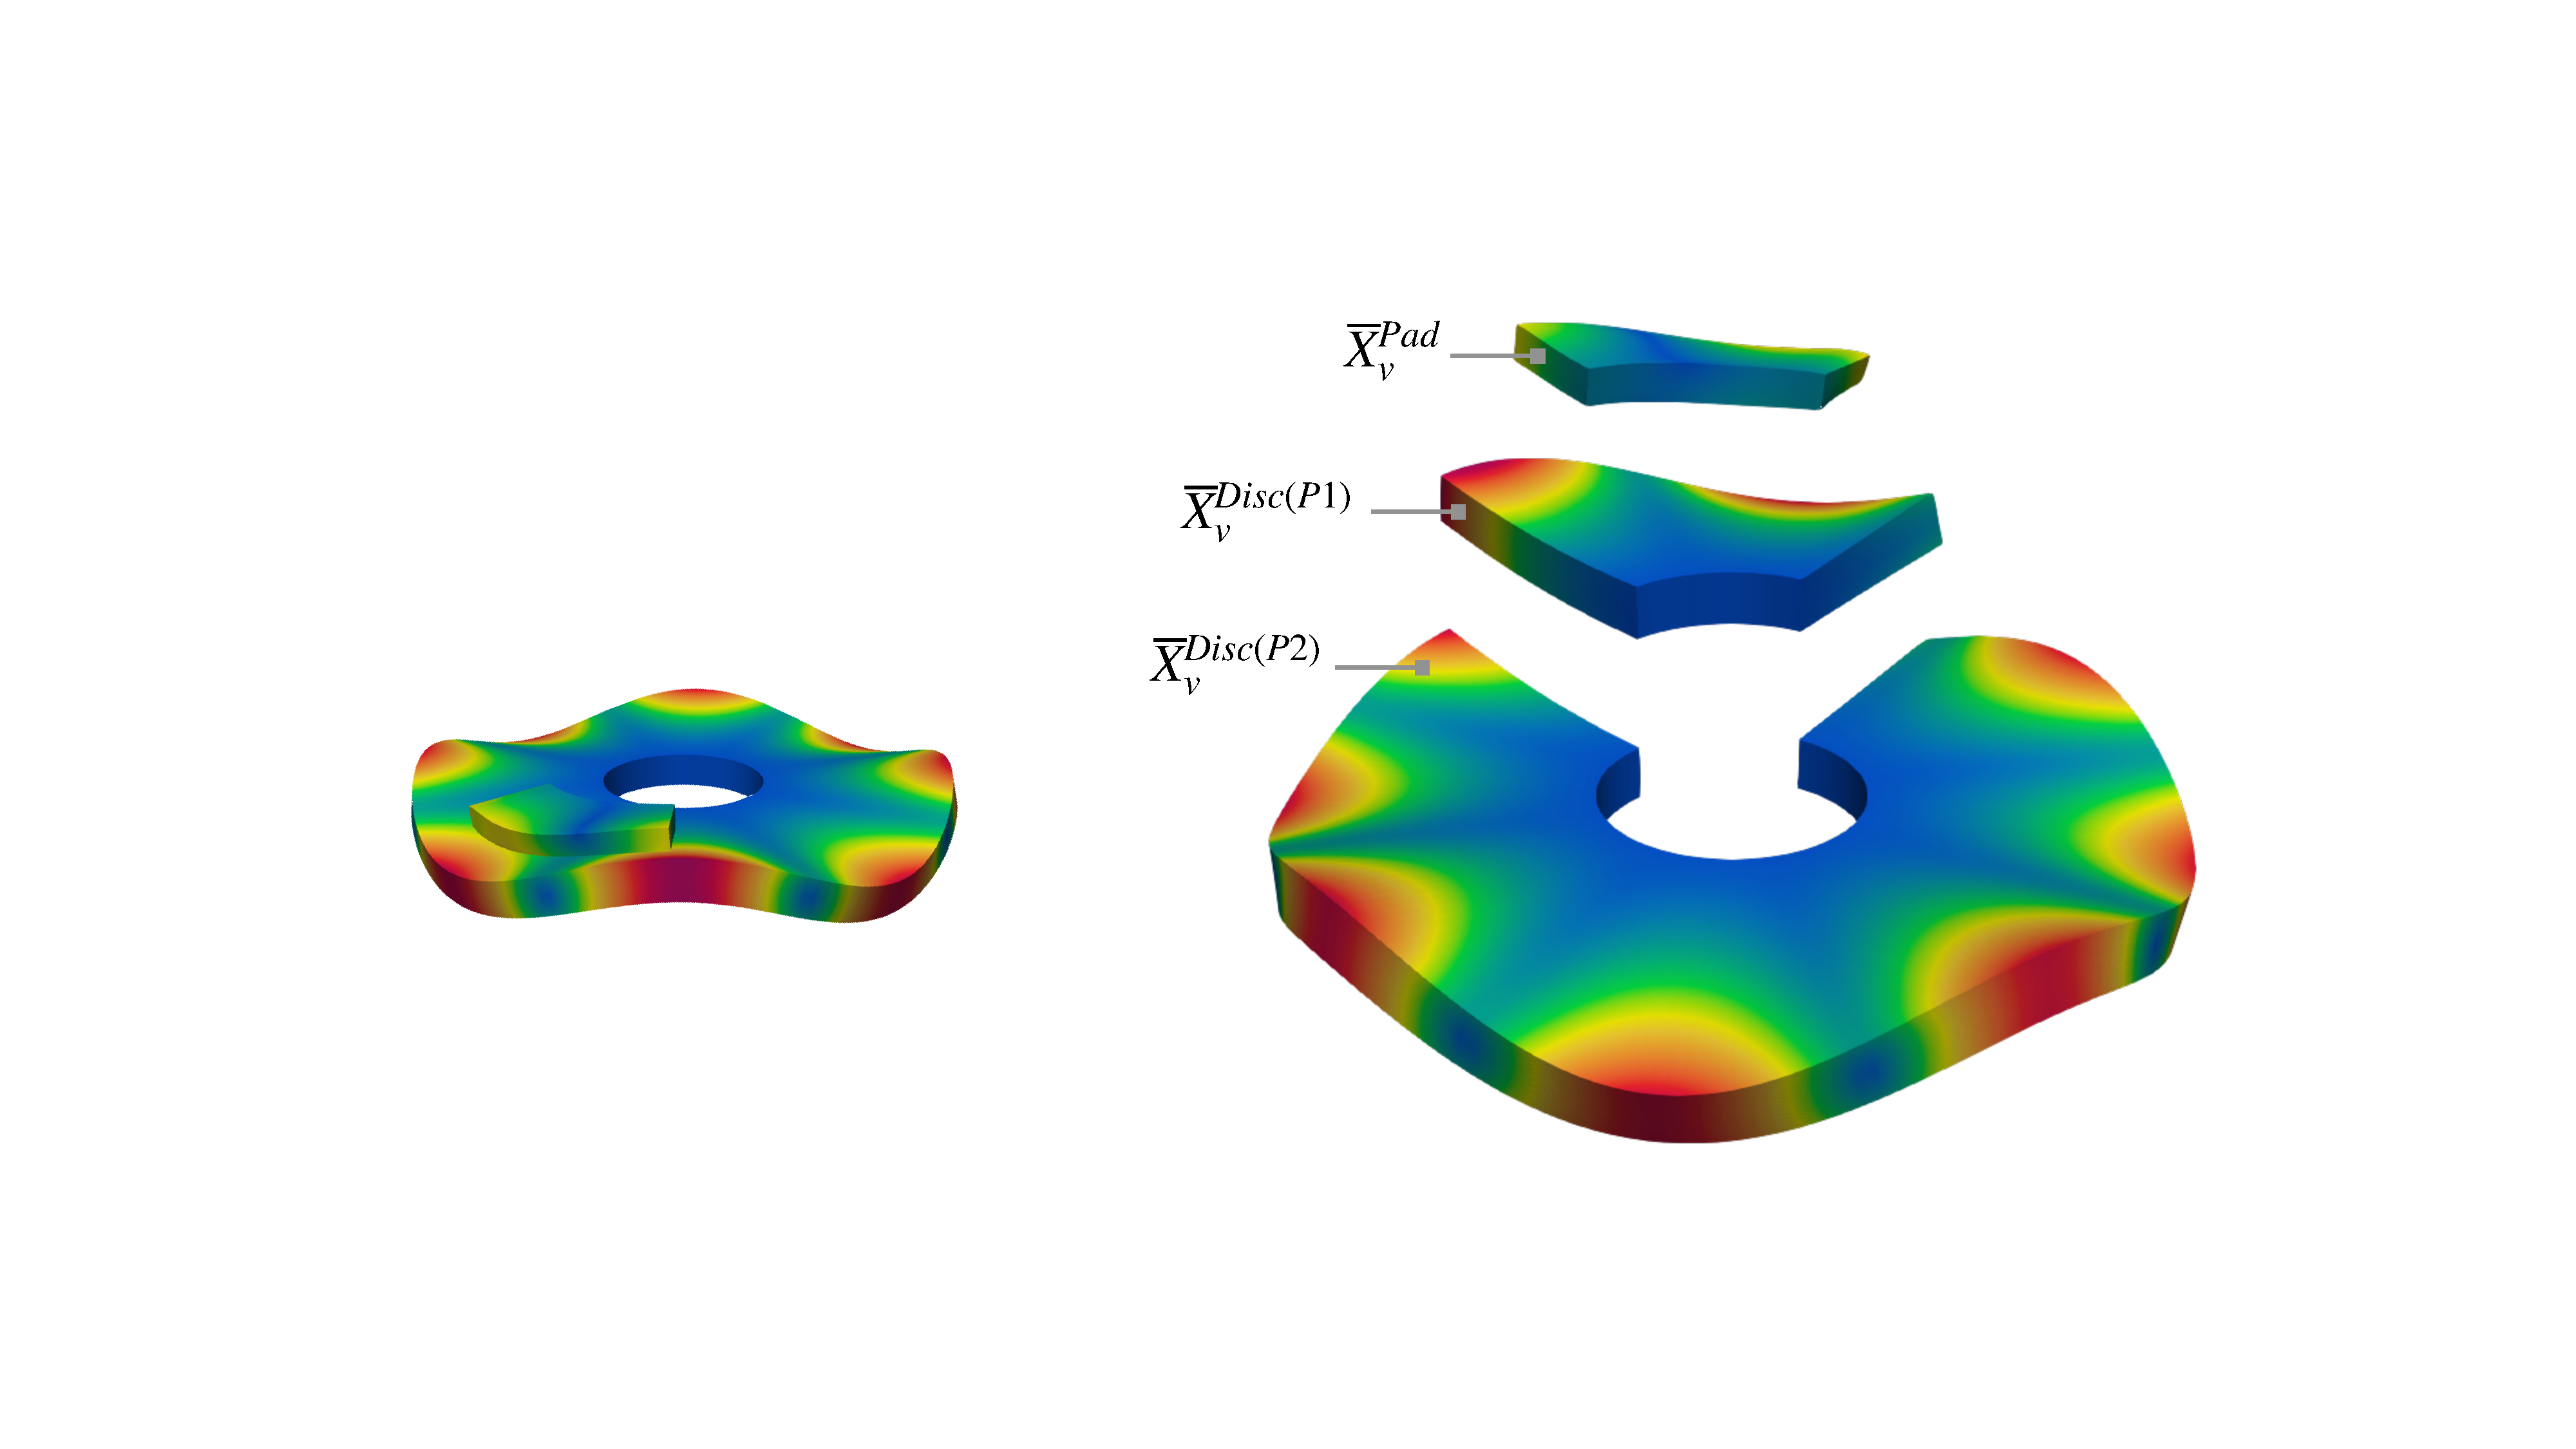
\includegraphics[scale=0.28]{Chapter5/Pictures/MP.pdf}
    \caption{Anatomy of parameterization for the disc-pad system with arbitrary dimensions, shown here for Mode 9, Frequency: 3630 Hz}
    \label{fig:MP_anatom}
\end{figure}

%We adapted some techniques which was well suited for our domain and problem of interest. 
The multi-patch parameterization of $\Omega^{(\mathrm d)}$ to break the NURBS tensor product definition is shown in Figure \ref{fig:multi-patch_disc}, where one patch  $\overline{X}_{v}^{(\mathrm d_1)}$ contains the contact domain $\Gamma_{C}^{(\mathrm d_1)}$ defined through a fine mesh by $h$-refinement and the other patch $\overline{X}_{v}^{(\mathrm d_2)}$ with a relatively coarse mesh sufficient to capture the required dynamic properties. And different strategies were used to reduce the solution smoothness induced by the continuity of the NURBS approximation across the boundary $\partial \Gamma_{C}^{(\mathrm d_2)}$ where typically strong solution gradient exists. For pad shapes where the knot lines on  $\overline{X}_{v}^{(\mathrm d_1)}$ can be aligned with $\partial\Gamma_{C}^{(\mathrm d_1)}$, $h$-refinement can be used with finer refinement around $\partial\Gamma_{C}^{(\mathrm d_1)}$, while the contact domain $\Gamma_{C}^{(\mathrm d_1)}$ itself is discretized by $h$-refinement through a relatively coarse mesh compared to the refinement around $\partial\Gamma_{C}^{(\mathrm d_1)}$, but finer than the rest of the domain. For pad shapes where the knot lines on $\overline{X}_{v}^{(\mathrm d_1)}$ cannot be aligned with the boundary $\partial\Gamma_{C}^{(\mathrm d_1)}$, we purely relied on $h$-refinement with much finer refinement. For the shape optimization, we used the later strategy due to random definition of shapes. \\


\begin{figure}[h!]
    \centering
    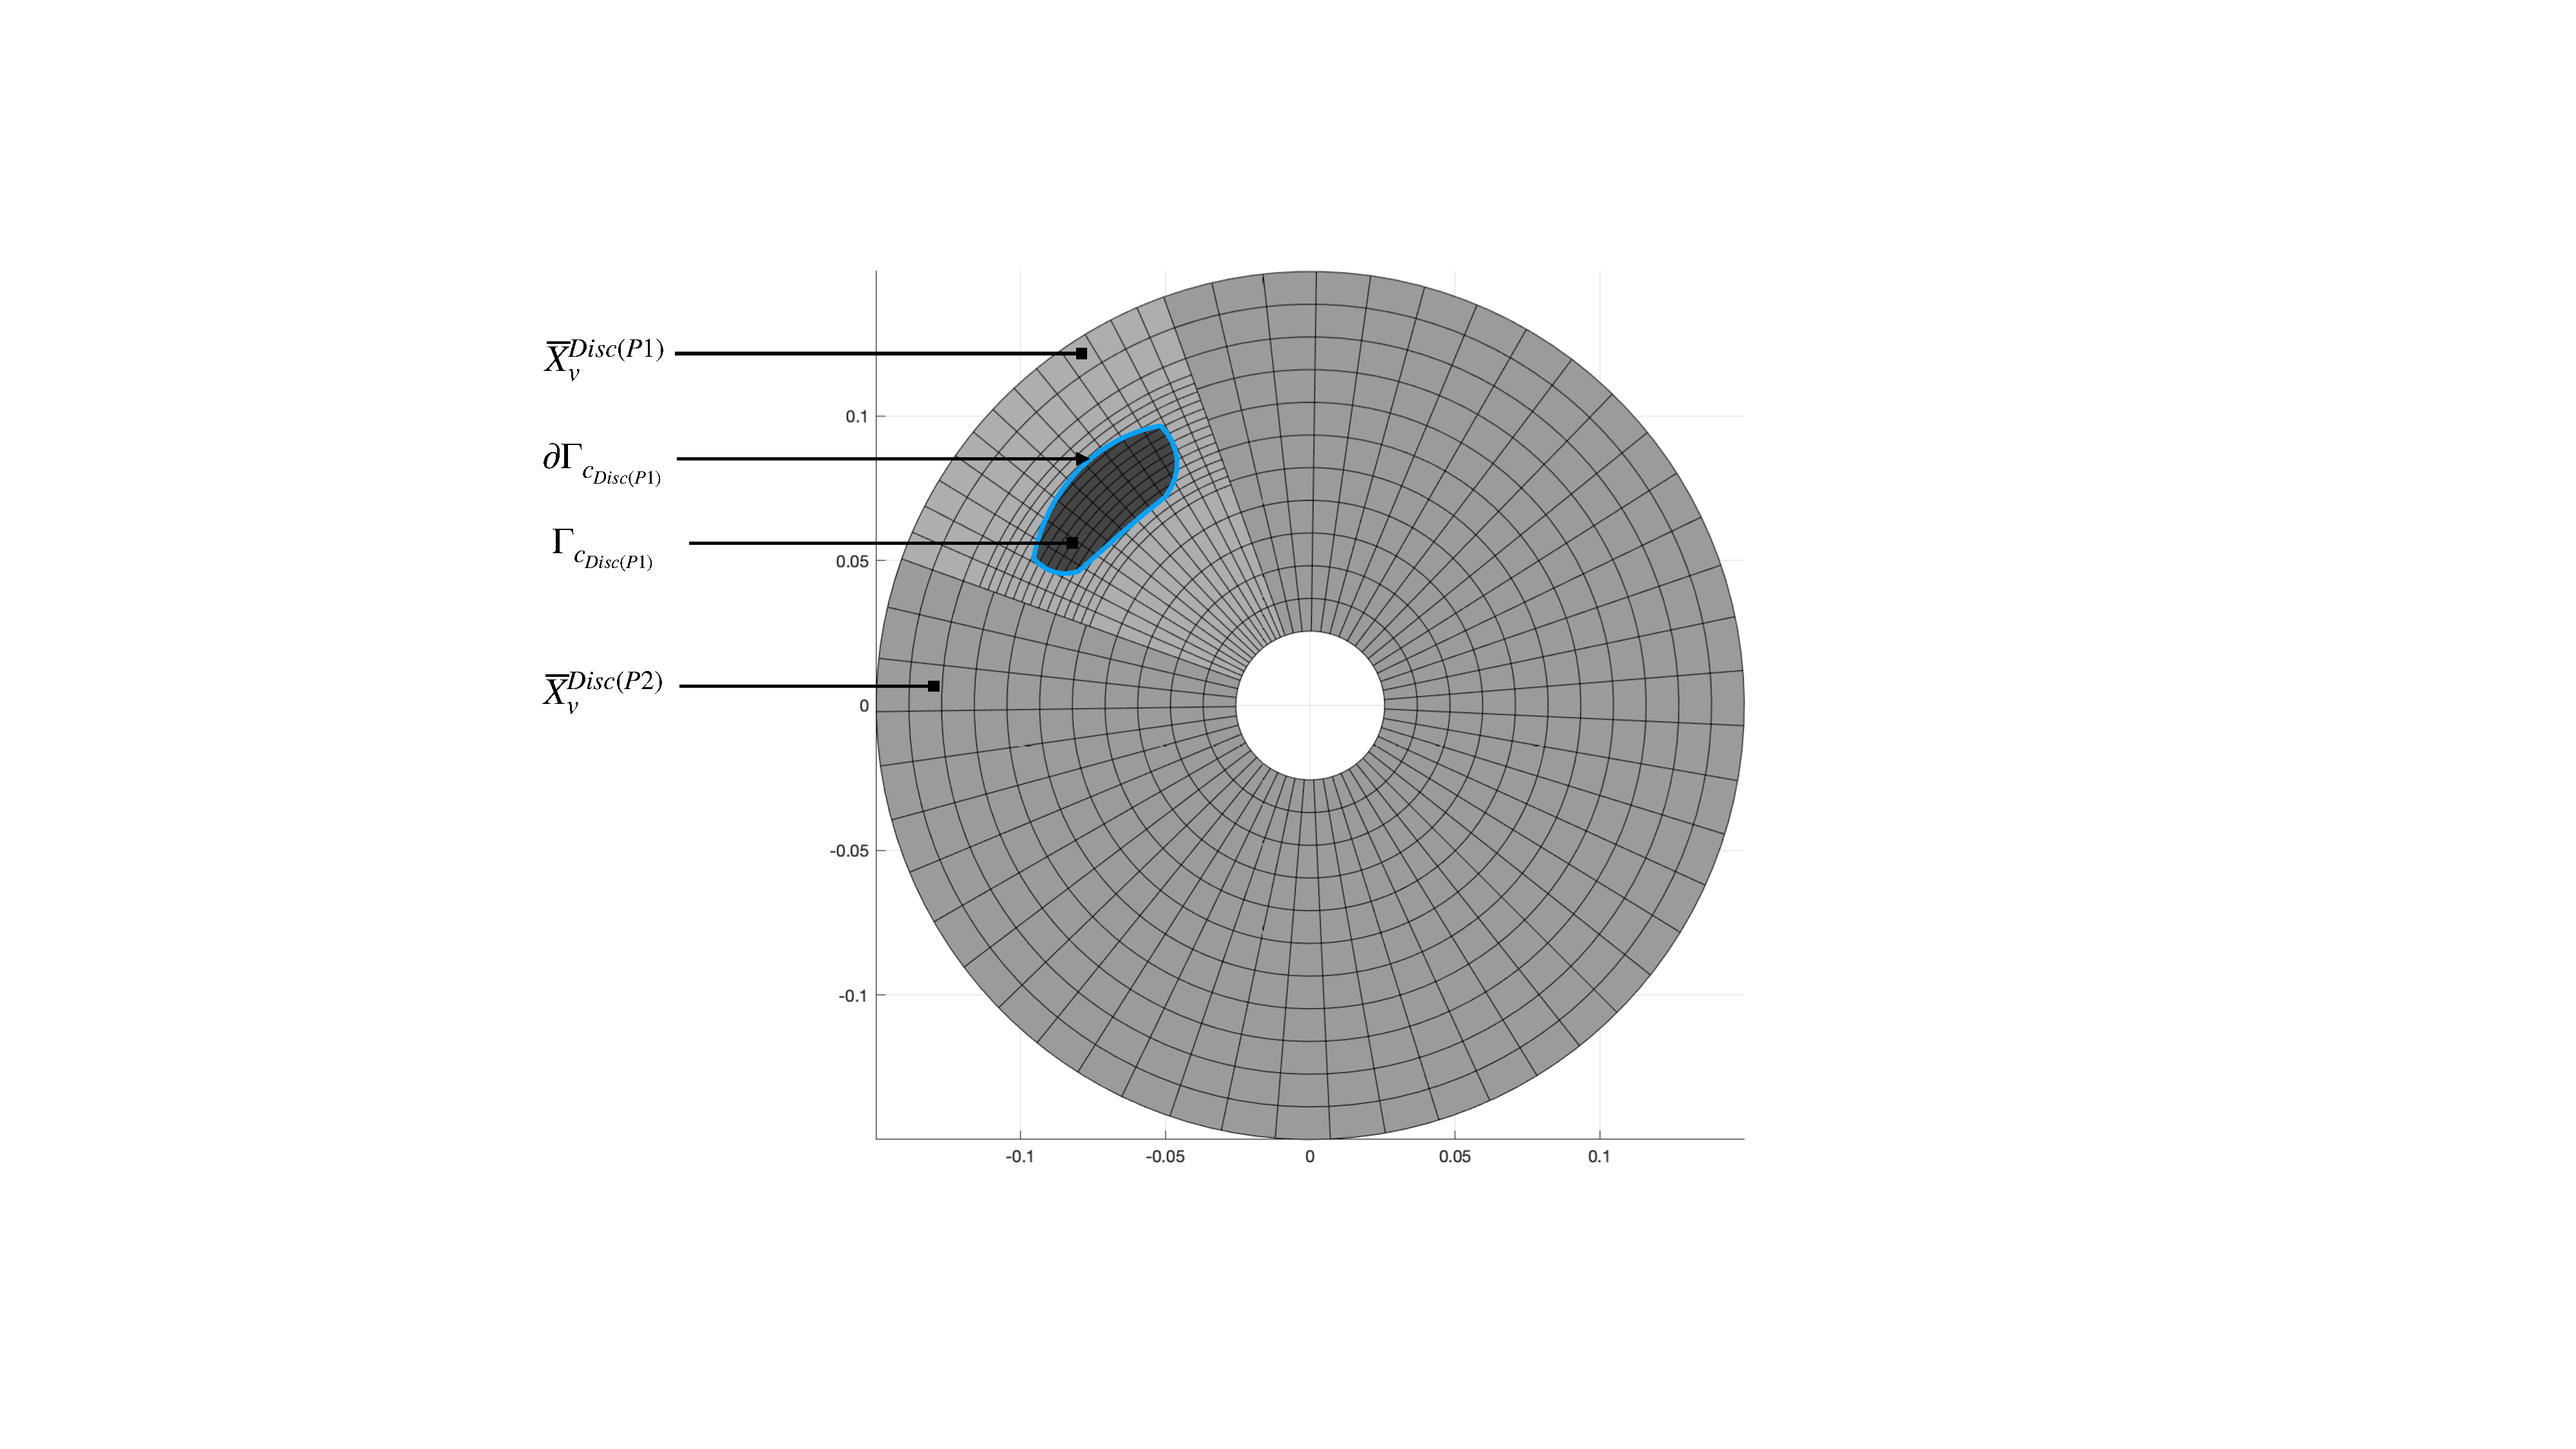
\includegraphics[scale=0.3]{Chapter5/Pictures/ran3.pdf}
    \caption{Multi-patch parameterization of $\Omega_{Disc}$ as $\overline{X}_{v}^{Disc}:=X_{v}^{Disc(P1)}(\xi,\eta,\zeta) \cup X_{v}^{Disc(P2)}(\xi,\eta,\zeta)$, with $h$-refinement at the contact region $\Gamma_{c_{Disc(P1)}}$.}
    \label{fig:multi-patch_disc}
\end{figure}

%As aforementioned, the pad is defined through a single patch parameterization $X_{v}^{Pad}(\xi,\eta,\zeta)$.
%In the optimization loop, for arbitrary definition of pad shapes, the parameterization was adapted for change in shape through $r$-refinement strategy i.e, the number of control points except for their positions are fixed. 
%Further, in the optimization loop, the dimension of the disc patches were adapted for changes in $\Gamma_{c_{Disc(P1)}}$ to realize a more restrictive local refinement on $\Gamma_{c_{Disc(P1)}}$ and across $\partial\Gamma_{c_{Disc(P1)}}$. Hence, the knot vectors were also adapted to have uniform spacing of knots for a given region irrespective of the change in the dimension of the patches. 

%While the multi-patch parameterization of $\Omega^{(\mathrm d)}$ makes it computationally efficient with defining local refinement on $\Gamma_{C}^{(\mathrm d_1)}$ and across $\partial\Gamma_{C}^{(\mathrm d_1)}$, 


 
 

\subsection{Bayesian optimization}

Bayesian optimization is an effective strategy for optimising computationally expensive objective functions \cite{Shahriari}. 

We begin the following explanations without defining the specifics of modelling the probability $\mathcal{P}$ which is given as knowledge and considering the optimisation of a single function $f(\bm{x})$ for $\underset{\bm x \in \mathcal{X}}{min}\,f(\bm{x})$.
The idea is based on Bayes rule where the prior knowledge $\mathcal{P}(\mathcal{H})$ of the hypothesis $\mathcal{H}$ and the likelihood of the evidence $\mathcal{E}$ given the hypothesis, $\mathcal{P}(\mathcal{E}|\mathcal{H})$, are used to infer the posterior knowledge of the hypothesis given the evidence, $\mathcal{P}(\mathcal{H}|\mathcal{E})$, where the proportionality is expressed as follows

\begin{equation}\label{Baye1}
\mathcal{P}(\mathcal{H}|\mathcal{E}) \propto \mathcal{P}(\mathcal{E}|\mathcal{H})\mathcal{P}(\mathcal{H})
\end{equation}

 where $\mathcal{P}(\mathcal{H}|\mathcal{E})$ defines Bayesian inference. In our setting, the hypothesis $\mathcal{H}$  corresponds to the function $f(\bm{x})$ and the evidence $\mathcal{E}$ to $\mathcal{F}_{1:{\mathfrak{n}}}:\{f(\bm{x}_1),f(\bm{x}_2),\hdots,f(\bm{x}_{\mathfrak{n}})\}$ where $f(\bm{x})$ is sampled on $\mathcal{X}_{1:{\mathfrak{n}}}:\{\bm{x}_1,\bm{x}_2,\hdots,\bm{x}_{\mathfrak{n}}\}$, with $\mathcal{D}_{1:{\mathfrak{n}}}:\{\mathcal{X}_{1:{\mathfrak{n}}},\mathcal{F}_{1:{\mathfrak{n}}}\}$. This is typically known as function-space view, since the probability is defined on the space of functions. It can be hard to conceptualise such view with functions, but it is possible if one can imagine the existence of a function in a mere probabilistic sense such that the random draw from a probability distribution is a function.  The relation \eqref{Baye} can be expressed in this case as\\
 
 \begin{equation}\label{Baye}
\mathcal{P}(f(\bm{x})|\mathcal{D}_{1:{\mathfrak{n}}}) \propto \mathcal{P}(\mathcal{D}_{1:{\mathfrak{n}}}|f(\bm{x}))\mathcal{P}(f(\bm{x}))
\end{equation}

 
 %The posterior knowledge can be then used to infer the optimum of the function where the expensive computational model needs to be evaluated. The new evaluation is then used to update the  belief of the prior, and with the likelihood to infer a new posterior. The process is run subsequently for optimization with the expectation of reaching the global optimum for the function. The most common method to model the prior of a function is through Gaussian process, which also infers the posterior as Gaussian. This is more efficient since this presents the prediction and the uncertainty of the prediction, which provides a decisive knowledge to construct an acquisition function to sample more efficiently for optimization.\\

%The modelling of prior, and the inference of posterior, for a function to be approximated takes the role of surrogate modelling commonly known as Gaussian process regression or Kriging. There are different context through which the Gaussian process regression could be presented owing to its diverse origins. We present in the context of function space view of Gaussian processes, but the interested readers can refer to the following articles for more details  \citep{Rasmussen1}\citep{Forrester}. Followed by, we present an acquisition function where we adapted  Expected Improvement($EI$) that defines EGO \citep{Jones1998}.\\
 
The prior over a function, $\mathcal{P}(f(\bm{x}))$, is typically modelled through spatial correlation which is assumed to be known a priori, where the hypothesis is that a given function exhibits certain characteristics of spatial correlation which can be generalized globally. 
In other words, a prior belief is defined over the space of functions, such that the functions in the space largely exhibit certain characteristics of spatial correlation. % which the function to be optimised is believed to exhibit. 
 With the prior $\mathcal{P}(f(\bm{x}))$ defined, and given the likelihood of the points sampled on the function, $\mathcal{P}(\mathcal{D}_{1:{\mathfrak{n}}}|f(\bm{x}))$, the posterior knowledge of the function, $\mathcal{P}(f(\bm{x})|\mathcal{D}_{1:{\mathfrak{n}}})$, can be inferred from the relation \eqref{Baye}. 
 The posterior knowledge $\mathcal{P}(f(\bm{x})|\mathcal{D}_{1:{\mathfrak{n}}})$ is then used to infer the next point $\bm{x}_{\mathfrak{n}+1}$ to be sampled, depending on the strategy set for sampling in optimization. 
 The sampled point $\bm{x}_{\mathfrak{n}+1}$ is then used to update the belief of the prior $\mathcal{P}(f(\bm{x}))$ in the light of $\mathcal{D}_{1:{\mathfrak{n}+1}}$, and with the likelihood $\mathcal{P}(\mathcal{D}_{1:{\mathfrak{n}+1}}|f(\bm{x}))$ to infer a new posterior $\mathcal{P}(f(\bm{x})|\mathcal{D}_{1:{\mathfrak{n}+1}})$, which characterizes active learning. 
 The process is run subsequently with the prospect of finding the global optimum for the function through active learning, defines Bayesian optimization.\\

With the general idea defined for Bayesian optimization, at least in the context of optimizing a single function, we can now define the notion of modelling $\mathcal{P}$ which is typically defined through Gaussian process ($\mathcal{GP}$). 
While a Gaussian distribution defines distribution over a random variable or in the case of a multi-variate Gaussian distribution over random variables, a $\mathcal{GP}$ defines distribution over a function, such that each draw from a $\mathcal{GP}$ is a function. 
For some intuition of the following explanations, this can be thought in a discrete sense as all the points, of a function drawn from a $\mathcal{GP}$ as being related through a dependent multi-variate Gaussian distribution such that each point is a univariate Gaussian distribution over a value of the function.\\

The prior over a function can hence be defined as $\mathcal{GP}$ prior, where the advantage of modelling the prior as Gaussian means that it preserves the conditioning of the Gaussian prior given the likelihood to infer the posterior as Gaussian as well. This is advantageous for Bayesian optimisation, since inferring the posterior as Gaussian presents the prediction as mean and the uncertainty of the prediction as variance, which provides a decisive knowledge to construct an acquisition function to sample more efficiently.\
The $\mathcal{GP}$ posterior defined through Bayesian inference from conditioning a $\mathcal{GP}$ prior given the likelihood of the sampled points over the function, characterizes a regression model, known as $\mathcal{GP}$ regression. Hence, the meta-modelisation of the function $f(\bm{x})$ can be defined through $\mathcal{GP}$ regression. \\

%Hence, it can be said in a probabilistic sense that a function with large variation between two arbitrary points for a given distance defined by a metric characterises weak spatial correlation, than a function with smaller variation for the same distance. The comparison can only be defined probabilistically, since different parts of the function can exhibit different spatial correlation, which means that characterising a function with respect to spatial correlation can also only be probabilistic. Even though, the knowledge of spatial correlation is assumed to be known a prior, it is often determined from the of light of the sampled data.  
%From a function-space view, $\mathcal{P(H)}$ can be defined as distribution over functions, where the distribution largely corresponds to functions which exhibit certain characteristics of spatial correlation. 
 %More on the mathematical specifics for defining the prior probabilistically will be shown in the upcoming explanations.\\
 
%Given the prior defined through spatial correlation for a function, and with the points sampled on the function, the posterior knowledge of the function can be inferred from the relation \eqref{Baye}.
%The posterior knowledge is then used to determine the next point to be sampled, where the process of determining a sample point is typically achieved through optimising an acquisition function. More on the role of acquisition function in optimization will be discussed later. 
%The sampled point is then used to update the belief of the prior, and with the likelihood to infer a new posterior. 
%The process is run subsequently which defines Bayesian optimization with the expectation of reaching the global optimum for the function. This is helpful for computationally expensive functions when often the computational resources are limited, where applying the classical optimization strategies cannot converge with the reduced number of evaluations.\\

 %With the general idea behind Bayesian optimization at least in the context of single objective optimization, we can now define the notion of modelling $\mathcal{P}(.)$ which is typically defined through Gaussian: $\mathcal{N}({\mu},{\sigma}^2)$. 
% While a Gaussian distribution defines distribution over a random variable or in the case of a multi-variate Gaussian distribution over random variables, a Gaussian process $\mathcal{GP}$ defines distribution over a function. 
 %Hence, the prior over a function is given as $\mathcal{GP}$ prior, where the advantage of modelling the prior as $\mathcal{GP}$ means that it infers the posterior as $\mathcal{GP}$ as well. 
 %Inferring the posterior as Gaussian presents the prediction and the uncertainty of the prediction, which provides a decisive knowledge to construct an acquisition function to sample more efficiently for optimization, where the optimization is explicity Bayesian.\\
%Before moving on to the notion of Gaussian distriubtion over functions, the fundamental properties relating to Gaussian are preserved, such that if the prior is assumed to be of Gaussian and the conditioning of a Gaussian results in a . This means that

 %Unlike other regression models, $\mathcal{GP}$ regression is seen as non-parametric since it does not assume a parametric form \footnote{The assumption of parametric form is also possible in Gaussian process regression through parametric form defined as mean function} on functions, where the parametric form is defined through a fixed number of parameters as coefficients of polynomial bases. This is advantageous since this eliminates the need for assuming a priori form of the bases to characterize a function which might be too demanding especially for black-box functions. Instead, the hyperparameters are involved in the covariance function for characterising spatial correlations, which means that a priori assumption for the covariance function and its associated parameters should be made. Definition of hyperparameters is non-parametric in a sense that it characterizes function... 
 
  
 %Add content for weight-space view
The $\mathcal{GP}$ prior $\mathcal{P}(f(\bm{x}))$ over $f(\bm{x})$ can be expressed as

\begin{multline}
f(\bm{x}) \approx \mathcal{P}(f(\bm{x})) = \mathcal{GP} ({\mu}(\bm{x}),k(\bm{x},\bm{x}^{'})),\\
{\mu}(\bm{x}) = \mathrm{E}[f(\bm{x})],\quad
k(\bm{x},\bm{x}^{'})=\mathrm{E}[(f(\bm{x})-\mu(\bm{x}))(f(\bm{x}')-\mu(\bm{x}'))]
\end{multline}
 
where the distribution constitutes a mean function $\mu(\bm{x})$ and a covariance function $k(\bm{x},\bm{x}^{'})$. The function $\mu(\bm{x})$ can be seen as the deterministic part which captures the general trend of $f(\bm{x})$, while the covariance function $k(\bm{x},\bm{x}^{'})$ models the stochastic trend which is the spatial correlation between any $f(\bm{x})-\mu(\bm{x})$ and $f(\bm{x}')-\mu(\bm{x}')$. 
The deterministic part $\mu(\bm{x})$ is largely modelled as a constant or through polynomials, which is demanding to estimate a priori and also higher degree polynomial trend functions can lead to overfitting over the sampled points. Hence, care should be taken in defining the general trend such that some spatial correlation exists with respect to the trend. Recently, focus has also been in defining $\mu(\bm{x})$ with Polynomial chaos expansion approach.\\

The spatial correlation is modelled by hyperparameters $\bm\theta$ which are the constants known a priori in a covariance function $cov(f(\bm{x})-\mu(\bm{x}),f(\bm{x}')-\mu(\bm{x}'))$, where the choice of the covariance function depends on the application. Even though the prior knowledge is defined to be known, it is often determined from the light of the sampled points. Hence, to define the prior over $k(\bm{x},\bm{x}^{'})$, the hyperparameters are estimated a priori from the sampled points, which is usually achieved by optimising the likelihood function for  $arg \, max_{\bm\theta} \,\, L(\mathcal{F}|\bm\theta)$. More on optimising for hyperparameters will be detailed in the upcoming explanations, where  $\bm\theta$ often contains parameters to model $\mu(\bm{x})$ in addition to the hyperparameters.\\

With $\bm\theta$ determined, the $\mathcal{GP}$ prior $\mathcal{P}(f(\bm{x}))$ can now be defined. The conditioning of $\mathcal{P}(f(\bm{x}))$ with the likelihood of the sampled points $\mathcal{D}_{1:{\mathfrak{n}}}$ results in a $\mathcal{GP}$ posterior $\mathcal{P}(f(\bm{x})|\mathcal{D}_{1:{\mathfrak{n}}},\bm\theta)$ which can be viewed in a finite-dimensional sense as the posterior joint Gaussian distribution of $\mathcal{P}(f(\bm{x}_1^*)),\mathcal{P}(f(\bm{x}_2^*)),\hdots,\mathcal{P}(f(\bm{x}_\mathfrak{.}^*))$ across rest of the function where its arguments $\bm{x}_\mathfrak{i}^*$ has not been sampled, i.e. $\bm{x}_\mathfrak{i}^* \notin \mathcal{X}_{1:{\mathfrak{n}}}$.\\
 
 To move on from the abstractness of  $\mathcal{GP}$ to a practical finite-dimensional Gaussian distribution useful for making inference at an arbitrary point  $\bm{x}^*\in \mathcal{X}$, given the sampled points $\mathcal{X}_{1:{\mathfrak{n}}}$, the properties of multi-variate Gaussian distribution allow to isolate a part of the $\mathcal{GP}$ prior $\mathcal{P}(f(\bm{x}))$ to define a joint Gaussian distribution of only the sampled points $\mathcal{X}_{1:{\mathfrak{n}}}$ and an argument $\bm{x}^*$ where the inference is to be made, where the joint distribution can be expressed as 
 
 \begin{equation}
  \begin{bmatrix}\mathcal{P}(f(\bm{x}_1)) \\\vdots\\\mathcal{P}(f(\bm{x}_n)) \\\mathcal{P}(f(\bm{x}^*)) \end{bmatrix}=\mathcal{N} \left( 
  \begin{bmatrix}
  \mu(\bm{x}_1) \\\vdots\\\mu(\bm{x}_\mathfrak{n}) \\\mu(\bm{x}^*) 
  \end{bmatrix},
%  
  \begin{bmatrix} 
k(\bm{x}_1,\bm{x}_1) &\hdots & k(\bm{x}_1,\bm{x}_\mathfrak{n}) & k(\bm{x}_1,\bm{x}^*)\\ 
\vdots & \ddots & \vdots & \vdots\\ 
k(\bm{x}_\mathfrak{n},\bm{x}_1)  &\hdots & k(\bm{x}_\mathfrak{n},\bm{x}_\mathfrak{n}) & k(\bm{x}_\mathfrak{n},\bm{x}^*)\\
k(\bm{x}^*,\bm{x}_1)  &\hdots & k(\bm{x}^*,\bm{x}_\mathfrak{n}) & k(\bm{x}^*,\bm{x}^*)\\
\end{bmatrix} \right)
\label{Joint_dist}
  \end{equation}
  
  The above joint distribution can be partitioned to define the mean and the covariance for the sampled points and the point to be inferred as
  
  \begin{equation}
{\bm{\Sigma}} =  \begin{bmatrix} 
k(\bm{x}_1,\bm{x}_1) &\hdots & k(\bm{x}_1,\bm{x}_\mathfrak{n})\\ 
\vdots & \ddots & \vdots\\ 
k(\bm{x}_\mathfrak{n},\bm{x}_1)  &\hdots & k(\bm{x}_\mathfrak{n},\bm{x}_\mathfrak{n})\\
\end{bmatrix},
{\bm{\Sigma}}^* =  \begin{bmatrix} 
k(\bm{x}_1,\bm{x}^*)\\ 
\vdots\\ 
k(\bm{x}_\mathfrak{n},\bm{x}^*)\\
\end{bmatrix},
\bm\mu(\mathcal{X}) =   \begin{bmatrix}
  \mu(\bm{x}_1) \\\vdots\\\mu(\bm{x}_\mathfrak{n}) 
  \end{bmatrix}
\end{equation}

The conditioning of the joint distribution Eq.\eqref{Joint_dist} defined by the prior knowledge of $\bm\theta$ with the sampled data $\mathcal{D}$ gives the prediction for $\bm{x}^*$ as follows

\begin{equation}
\mathcal{P}(f(\bm{x}_i^*)|\mathcal{D},\bm\theta)=\mathcal{N}(\underbrace{\mu(\bm{x}_i^*)+\bm{\Sigma}^{-1}\bm{\Sigma}^*(\mathcal{F}-\bm\mu(\mathcal{X}))}_{\hat{\mu}(\bm{x}^*)},\underbrace{k(\bm{x}^*,\bm{x}^*)-\bm{\Sigma}^*\bm{\Sigma}^{-1}{\bm{\Sigma}^*}^{T}}_{\hat{\sigma}^2(\bm{x}^*)})
\end{equation}\\

where the function $f(\bm x)$ approximated by the Gaussian process regression model can be defined as $\hat{f}(\bm x):=\mathcal{N}(\hat{\mu}(\bm x),\hat{\sigma}(\bm x))$.\\

The choice of the covariance function and the estimation of the hyperparameters in defining spatial correlation are important since they are the determining factors that distinguish the above distribution for a given observation. The hyperparameters parameterizes spatial correlation through smoothness or correlation length or sometimes both \footnote{It should be noted that the parameters modelling smoothness and correlation length are not independent, but rather interdependent such that parameters modelling smoothness has influence on correlation length and vice-versa. But largely, smoothness parameters can be said to quantify the gradient factor for the variation of $h$, while correlation length parameters can be said to quantify the influence of the points on each other for the variation of $h$}, for which a large class of covariance functions exist to choose from depending on the application. The most commonly used in engineering optimisation are the Gaussian and the Matérn class of covariance functions, where for isotropic correlation, the Gaussian covariance function can be defined as 

\begin{equation}
 k(\bm{x},\bm{x}^{'}) = exp\bigg(-\frac{1}{2 \theta^2}||\bm{h}||^2\bigg)
\end{equation}

where $\bm h:=[h_1,h_2,\cdots,h_{\mathsf{l}}]$ , $h=(f({x})-\mu({x}))-(f({x}')-\mu({x}'))$ and $\bm x$ is considered to be in $\mathbb{R}^{\mathsf{l}}$. This is defined with only a single hyperparameter $\theta$ since it assumes the spatial correlation to be isotropic. The anisotropic consideration of spatial correlation can be defined as

\begin{equation}
 k(\bm{x},\bm{x}^{'}) = exp\bigg(-\sum_{\mathsf{k}=1}^{\mathsf{l}}\frac{1}{2\theta^2_{\mathsf{k}}}|h|^2\bigg)
\end{equation}

where it leads to determining $\mathsf{l}$ no. of $\theta$. The Gaussian covariance function models spatial correlation only with correlation length defined through the factor $\frac{1}{2\theta^2}$, while the smoothness for the variation of $h$ is defined for a fixed power $2$. The Matérn class of covariance functions provide flexibility in modelling smoothness through a predefined parameter $\upsilon$, where the function can be expressed for anisotropic variation as

\begin{equation}
 k(\bm{x},\bm{x}^{'}) = \sum_{\mathsf{k}=1}^{\mathsf{l}} \sigma^2 \frac{2^{(1-\upsilon)}}{\mathsf{G}(\upsilon)}\bigg(\frac{\sqrt{2\upsilon}|h_{\mathsf{k}}|}{\theta_{\mathsf{k}}}\bigg)^{\upsilon} \mathsf{B}\bigg(\frac{\sqrt{2\upsilon}|h_{\mathsf{k}}|}{\theta_{\mathsf{k}}}\bigg)
\end{equation}

where $\mathsf{G}$ and $\mathsf{B}$ are the Gamma function and the Bessel function of order $\upsilon$ respectively. The value of $\upsilon$ is typically defined to be $5/2$ or $3/2$, where as $\upsilon \rightarrow \infty$, it converges to squared exponential function and for $\upsilon = 1/2$, it simply characterizes an exponential function. The Gaussian covariance makes strong smoothness assumption with the infinite differentiability of the function which can be unreal and hence, Matérn class of functions are typically preferred which are $\upsilon-1$ times differentiable. We used Matérn with $\upsilon=5/2$, expressed as

\begin{equation}
 k(\bm{x},\bm{x}^{'}) = \sum_{\mathsf{k}=1}^{\mathsf{l}} \sigma^2 \bigg( 1+\frac{\sqrt{5}|h_{\mathsf{k}}|}{\theta_{\mathsf{k}}}+\frac{5h^{2}}{3\theta_{\mathsf{k}}^2}\bigg)exp\bigg(-\frac{\sqrt{5}|h_{\mathsf{k}}|}{\theta_{\mathsf{k}}}\bigg)
\end{equation}

With the definition of a covariance function, the optimisation of the hyperparameters to model the prior \eqref{Joint_dist} is given by $arg \, max_{\bm\theta} \,\, L(\mathcal{F}|\bm\theta)$, where $L(\mathcal{F}|\bm\theta)$ defines the likelihood of the observed data given the hyperparameters, defined by the joint probability as

\begin{equation}
L(\mathcal{F}|\mu(\bm{\theta}),\sigma({\bm \theta}))= \frac{1}{\sqrt{(2\pi\sigma^2)^{n}|\bm\Sigma|}}exp\bigg[-\frac{(\mathcal{F}-\bm{\mu}(\mathcal{X}))^T\bm\Sigma^{-1}(\mathcal{F}-\bm{\mu}(\mathcal{X})}{2\sigma^2} \bigg] 
\end{equation}

In optimising the above function for maximum likelihood, the function can be simplified by taking the natural logarithm while preserving the monotonicity of the function as

\begin{equation}\label{ln_like}
 ln(L)=-\frac{n}{2}ln(2\pi)-\frac{n}{2}ln(\sigma^2)-\frac{1}{2} ln|\bm\Sigma|-\frac{(\mathcal{F}-\bm{\mu}(\mathcal{X}))^T\bm\Sigma^{-1}(\mathcal{F}-\bm{\mu}(\mathcal{X}))}{2\sigma^2}
 \end{equation}

The definition of the logarithm preserves the monotonicity of the function and hence also the optimum point of the function.
Mean can be defined as $\bm \mu = \mathsf{X}\bm \theta_{\bm \mu}$ when modelled as regression with hyperparameters $\bm \theta_{\bm \mu}$ \footnote{$\bm\theta:=\{ \bm\theta_{\bm \mu}\}\cup\{\bm \theta_{\bm \Sigma}\}$, where $\bm\theta_{\bm \mu}$ and $\bm \theta_{\bm \Sigma}$ correspond to the hyperparameters of $\bm \mu$ and $\bm \Sigma$}, where $\mathsf{X}$ defines a matrix of size $\mathfrak{n}\times\mathsf{p}$, with $\mathsf{p}$ being the number of linear combination of functions defined for regression. The maximum likelihood estimate of $ \bm \mu$ in this case is simply the maximum likelihood estimate of $\bm {\theta_{\bm \mu}}$ which can be deduced from $\frac{\partial ln(L)}{\partial \bm {\theta_{\bm \mu}}} =0$ as

\begin{equation}
\bm {\check{\theta}_{\bm \mu}}=(\mathsf{X}^T \bm\Sigma^{-1}\mathsf{X})^{-1}\mathsf{X}^T \bm\Sigma^{-1}\mathcal{F}
\end{equation} 

which is simply the minimiser for generalized least-squares. This is apparent, since the minimiser of $\bm {\theta_{\bm \mu}}$ can be viewed as the minimisation of the generalised least-squares problem given as

\begin{equation}
\bm {\check{\theta}_{\bm \mu}} = arg\,{min}_{{\bm\theta_{\bm \mu}}} \frac{(\mathcal{F}-\bm{\mu}(\mathcal{X},{{\bm\theta_{\bm \mu}}}))^T\bm\Sigma^{-1}(\mathcal{F}-\bm{\mu}(\mathcal{X},{{\bm\theta_{\bm \mu}}}))}{2\sigma^2}
\end{equation} 

 Similarly, the maximum likelihood estimate for $\sigma$ can be defined from $\frac{\partial ln(L)}{\partial \sigma} =0$ as

\begin{equation}
\check{\sigma} =(\mathcal{F} - \mathsf{X}\bm\theta_{\bm \mu})^T\bm\Sigma^{-1}(\mathcal{F} - \mathsf{X}\bm \theta_{\bm \mu})
\end{equation}

Substituting the maximum likelihood estimates of $\check{\bm \theta}_{\bm \mu}$ and $\check{\sigma}$ in to Eq.{\eqref{ln_like}}, and with the constants removed as affine terms, one obtains

\begin{equation}\label{max_ln}
ln(L(\bm \theta)) \approx -\frac{n}{2}ln(\check{\sigma}^2(\bm \theta))-\frac{1}{2}ln|\bm \Sigma(\bm \theta_{\bm \Sigma})|
\end{equation}

The above function can be typically expected to be multimodal and hence the optimisation is typically achieved with Genetic algorithm (GA) for global convergence, followed by the best individuals from the GA as seeds for the quasi-newton algorithms like BFGS for local convergence. As a variation, quasi-newton schemes are also applied with in GA for the best individuals in each generation to define the parent population of the next generation.\\



The Bayesian inference $\mathcal{P}(f(\bm{x}_i^*)|\mathcal{D}_{1:{\mathfrak{n}}},\bm\theta)$ can be used in sampling for optimisation from the inference of the prediction $\hat{\mu}(\bm{\bm{x}}^*)$ and the uncertainty $\hat{\sigma}^2(\bm{x}^*)$ of the prediction. Naturally, question arises for the goal of sampling in balance between exploration and exploitation. Exploration can viewed as the means to gain more knowledge about the function especially where high uncertainty is reflected by the $\mathcal{GP}$ posterior. But with pure exploration, it diverts the goal in search for a global optimum with the consequence of reducing the uncertainty over the knowledge of the function, unless reducing the uncertainty also exposes the global optimum as a repercussion which happens rarely.  In contrast, exploitation focuses on parts of the function which is inferred to define optimum through the prediction from the $\mathcal{GP}$ posterior. Pure exploitation in optimisation can be viewed as more optimistic with the predictions and hence can underestimate the uncertain parts reflected by the $\mathcal{GP}$ posterior.\\

 This is where sampling through an acquisition function plays an important role in guiding the search for optimisation where the construction of the acquisition function can be adapted to set the balance between exploration and exploitation depending on the objective, for which a wide range of acquisition functions exist. 
 In general, acquisition functions define improvement with respect to a reference value $f(\bm{x}^+)$ through a probabilistic metric, where $f(\bm{x}^+)$ typically corresponds to the utopian value \footnote{Utopian value is the observed optimum value of the function} of the function, at least in the context of single objective optimisation. 
 While in multi-objective optimisation the definition of utopian value corresponds to empirical Pareto front which will be discussed later. 
 We will introduce some of the acquisition functions for single-objective optimisation which will be referred for the upcoming explanations. As defined before, we consider the case of optimising $f(\bm{x})$ for $\underset{\mathcal{X}}{min}\,f(\bm{x})$ for the following explanations and hence the utopian value  $f(\bm{x}^{++})$\footnote{We use the notation $f(\bm{x}^{++})$ to define the Utopian value as reference value and $f(\bm{x}^{+})$ to define an arbitrary reference value} is defined by ${\bm x}^{++}=arg \, min_{\bm{x}_{\mathfrak i}\in\mathcal{X}_{1:\mathfrak{n}}} f(\bm x_{\mathfrak{i}})$.\\
 
  
 Probability of Improvement (PI) for any  $\mathcal{GP}$ outcome $\hat{f}(\bm x)$ is given as 
 
 \begin{equation}
 PI(\bm x) = \mathcal{P}({f}(\bm x)\leq f(\bm{x}^{++}))
 \end{equation}
 
 where,\\  
 
 \begin{equation}
 \mathcal{P}({f}(\bm x)\leq f(\bm{x}^+))=CDF\bigg(\frac{\hat{\mu}(\bm x)-f(\bm{x}^{++})}{\hat{\sigma}(\bm x)}\bigg)
 \end{equation}\\

$PI$ gives more weight on exploitation than exploration in optimisation. This can be seen with the following case, where for a point with low variance for $\hat{\mu}<f(\bm{x}^{++})$ reflects more scope for improvement than for a point with the same $\hat{\mu}$ but larger variance, where $PI$ reflects more focus on exploitation which leads to highly exhaustive search locally. $PI$ is the same when both  points have $\hat{\mu}=f(\bm{x}^{++})$ and when $\hat{\mu}>f(\bm{x}^{++})$, the point with larger variance has larger $PI$, where $PI$ reflects focus on exploration. This means that $PI$ focuses on exploration unless there is no possibility for exploitation, where in real world, this leads to exhaustive search locally around the best points before moving on to the next exploration search. To overcome this effect, a trade-off parameter $\mathscr{E}\geq 0$ is introduced, given as

 \begin{equation}\label{PI_e}
 PI(\bm x) = \mathcal{P}({f}(\bm x)\leq f(\bm{x}^{++})+\mathscr{E})
 \end{equation}
 
 where typically $\mathscr{E}$ is set to be higher initially in an optimisation to drive exploration, and decreases to zero by the end of the optimisation to drive exploitation. $PI$ clearly lacks a good balance between exploration and exploitation for which Expected Improvement $EI$ is typically deemed to be effective.\\
 
 $EI$ is the expectation of the improvement,  $E(I(\bm x))$, where the improvement is typically defined with respect to the utopian value $f(\bm{x}^{++})$  as  $I(\bm x)= f(\bm{x}^{++})-\hat{f}(\bm x)$. The expectation of the improvement, $EI(\bm x|f(\bm{x}^{++}))$ \footnote{For simplicity, we define $EI(\bm x|f(\bm{x}^{++}))$ as $EI(\bm x)$ unless we want to emphasize the use of $f(\bm{x}^{++})$} can hence be expressed as
 
 \begin{equation}\label{EI_raw}
EI(\bm x)=E(I(\bm x)) = \int_{-\infty}^{{f}(\bm x^{++})} I(\bm x)PDF\bigg( \frac{f(\bm{x}) - \hat\mu(\bm x))}{\hat\sigma(\bm x)} \bigg) d{f}(\bm x)
\end{equation}
 
 For intuition, the above expression can be given as 
 
 \begin{equation}\label{EI_cent}
EI(\bm x) =  \Bigg(f(\bm x^{++}) - \underbrace{\frac{\int_{-\infty}^{{f}(\bm x^{++})} f(\bm{x}) PDF\bigg( \frac{f(\bm{x}) - \hat\mu(\bm x))}{\hat\sigma(\bm x)} \bigg) d{f}(\bm x)}{CDF\bigg( \frac{f(\bm{x}^{++}) - \hat\mu(\bm x))}{\hat\sigma(\bm x)} \bigg)}}_{f_{cen}}\Bigg) CDF\bigg( \frac{f(\bm{x}^{++}) - \hat\mu(\bm x))}{\hat\sigma(\bm x)} \bigg)
\end{equation}
 
 where $f_{cen}$ is the first moment of area/centroid of the $PDF \bigg( \frac{f(\bm{x}) - \hat\mu(\bm x))}{\hat\sigma(\bm x)} \bigg) \in (-\infty,{f}(\bm x^{++})]$ on the axis of ${f}(\bm x)$. 
Hence, $EI$ can be understood as the measure of $f_{cen}$ with respect to the reference value $f(\bm x^{++})$, given as $f(\bm x^{++}) - f_{cen}$, weighted by the $CDF\bigg( \frac{f(\bm{x}^{++}) - \hat\mu(\bm x))}{\hat\sigma(\bm x)} \bigg)$ which is simply $PI(\bm x)$. 
The term ${\int_{-\infty}^{{f}(\bm x^{++})} f(\bm{x}) PDF\bigg( \frac{f(\bm{x}) - \hat\mu(\bm x))}{\hat\sigma(\bm x)} \bigg) d{f}(\bm x)}$ can be seen as the measure of $E(\hat{f}(\bm x))$ in the interval 
 $(-\infty,{f}(\bm x^{++})]$, where it defines the expected value rather than the expected improvement  defined by $EI$ with respect to a reference value.  We elaborate these definitions since it will be useful for definitions to extend $EI$ to MOO. \\
 
Overall, $EI$ provides better trade-off between exploration and exploitation, unlike the greedy nature of $PI$ which primarily focuses on exploitation. This is because the term $f(\bm x^{++}) - f_{cen}$ weighted by $PI$ provides the additional factor in $EI$ to balance the search for exploration. The above expression of $EI$ can be simplified as
 
\begin{equation}
EI(\bm x)=(f(\bm{x}^{++}) - \hat\mu(\bm x)) CDF\bigg( \frac{f(\bm{x}^{++}) - \hat\mu(\bm x))}{\hat\sigma(\bm x)} \bigg)+\hat\sigma(\bm x) PDF \bigg( \frac{f(\bm{x}^{++}) - \hat\mu(\bm x))}{\hat\sigma(\bm x)} \bigg)
\end{equation}
 
 Similar to Eq. \eqref{PI_e}, it is possible to control the trade-off between exploration and exploitation by introducing $\mathscr{E}\geq 0$ to the above expression as follows \\

\begin{equation}
EI(\bm x)=(f(\bm{x}^{++}) - \hat\mu(\bm x) -  \mathscr{E}) CDF\bigg( \frac{f(\bm{x}^{++}) - \hat\mu(\bm x))}{\hat\sigma(\bm x)} \bigg)+\hat\sigma(\bm x) PDF \bigg( \frac{f(\bm{x}^{++}) - \hat\mu(\bm x))}{\hat\sigma(\bm x)} \bigg)
\end{equation}\\

The other common acquisition function is defined with the bound of  $\hat{f}(\bm x)$, where for a function to be minimised, the  lower confidence bound can be defined as

\begin{equation}\label{lcb}
LCB(\bm x) = \hat{\mu}(\bm x) - \epsilon \hat\sigma(\bm x)
\end{equation}

 where $\epsilon \geq 0$. It is quite intuitive to think that $LCB$ favours exploration over exploitation. It is apparent that each acquisition function will give rise to distinct sampling behaviour and hence, the choice of the acquisition function depends on the goal for sampling. Similar to the approach of maximising Eq. \eqref{main_ln}, the optimisation of the acquisition functions can be achieved with the combination of GA and quasi-newton algorithms to determine the infill point $\bm x^{\iota}$.  
 
\subsubsection{Multi-objective optimisation}

For MOO, the problem can be formulated as

\begin{equation}
\underset{\bm x \in \mathcal{X}}{min} \, \bm f(\bm x)
\end{equation}\\

where $\bm f=[f_1(\bm x),\cdots, f_{\mathsf{m}}(\bm x)]$, $\bm f:\mathcal{X}\subset \mathbb{R}^{\mathsf{l}}\rightarrow \mathcal{S}\subset\mathbb{R}^{\mathsf{m}}$, with $\mathcal{S}$ being the objective space. The definition of optimality in single objective optimisation is defined with minimum or maximum of a function. While in MOO for a set of functions to be minimised, where typically the functions can not be minimised simultaneously without conflict between the objectives, where minimising one function can implicitly maximise the other. Hence, the definition of optimality in MOO is given by Pareto optimality which defines optimality considering the best compromise between the objectives.\\

Hence, any two vectors $\bm x_a,\bm x_b\in \mathcal{X}$, and  $\bm x_a \neq \bm x_b$, the following conditions can be stated for Pareto-dominance to define Pareto-optimality on $\underset{\bm x \in \mathcal{X}}{min} \, \bm f(\bm x)$, given as

\begin{itemize}
\item $\bm x_a \preceq \bm x_b \,\, (\bm x_a \, \mathrm{weakly\,\,dominates} \,\, \bm x_b)\,\, i.f.f. \,\, \forall \mathsf{i},\,\, f_{\mathsf{i}}(\bm x_a) \leq f_{\mathsf{i}}(\bm x_b)$

\item $\bm x_a \prec \bm x_b \,\, (\bm x_a \, \mathrm{dominates} \,\, \bm x_b) \,\, i.f.f. \,\, \bm x_a \preceq \bm x_b \,\, \& \,\, \exists \mathsf{i}\,\, s.t \,\,  f_{\mathsf{i}}(\bm x_a) < f_{\mathsf{i}}(\bm x_b)$

\item $\bm x_a  \sim \bm x_b \,\, (\mathrm{neither\,\,dominates\,\,the\,\,other}) \,\, i.f.f. \,\, \bm x_a \nprec \bm x_b \,\, \mathrm{and}\,\, \bm x_b \nprec \bm x_a$
\end{itemize}

where  $\mathsf{i}\in \{1,\cdots,\,\mathsf{m}\}$. Any $\bm x_a \in \mathcal{X}$ can be said as Pareto-optimal $i.f.f. \,\, \nexists \bm x_b \in \mathcal{X} \,\, s.t. \,\, \bm x_a \prec \bm x_b$, given $\bm x_b \neq \bm x_a$. Hence, the Pareto-optimal set/Non-dominated solutions(NDS) ${\mathscr{P}}$ and Non-dominated points (NDS)/Pareto-front $\bm f(\mathscr{P})$ can be defined as follows

\begin{itemize}
\item  ${\mathscr{P}}:=\{\bm x_a \in \mathcal{X} : \bm x_a \neq \bm x_b, \nexists  \bm x_b \in \mathcal{X} \,\, s.t. \,\, \forall \mathsf{i}, \,\, f_{\mathsf{i}}(\bm x_a) \leq f_{\mathsf{i}}(\bm x_b)\,\, \& \,\, \exists \mathsf{i} \,\, s.t \,\, f_{\mathsf{i}}(\bm x_a) \leq f_{\mathsf{i}}(\bm x_b) \}$
\item  $\bm{f} ({\mathscr{P}}):=\{\bm f(\bm x_a) \in \mathcal{S} : \bm x_a \neq \bm x_b, \nexists  \bm x_b \in \mathcal{X} \,\, s.t. \,\, \forall \mathsf{i}, \,\, f_{\mathsf{i}}(\bm x_a) \leq f_{\mathsf{i}}(\bm x_b)\,\, \& \,\, \exists \mathsf{i} \,\, s.t \,\, f_{\mathsf{i}}(\bm x_a) \leq f_{\mathsf{i}}(\bm x_b) \}$

\end{itemize}

Hence, Pareto-front in the context of MOO corresponds to the optimal solution of a function. Often distinguish is made between the true Pareto-front which corresponds to the true optimal of a function in single objective case and the observed Pareto-front known as empirical Pareto-front which corresponds to the known optimal of a function in single objective case. For the following definitions, we define NDS as empirical Pareto-front unless otherwise specified. Similar to the Utopian point in Single objective optimisation, Utopian point in MOO corresponds to a vector of all the known optimal solutions in $\mathcal{S}$. While the Nadir point defines the opposite, if the optimal points are defined to be the minimum of functions in MOO, Nadir point defines the maximum of all the functions in the NDS.\\

Before moving on to the Multi-objective Bayesian optimisation (MOBO), we introduce some of the standard approaches in MOO, since most of the approaches in MOBO has influence of the standard approaches where in MOBO typically acquisition functions are replaced for expensive functions and optimised in the context of MOO. Broadly MOO approaches can be classified in to two, where one approach typically converts MOO in to a set of single objective optimisations and optimise with classical single objective strategies. While the other approach works directly in the context of MOO, where Pareto-dominance measures are used directly in optimisation. The former approach is typically based on aggregation procedures, where a vector of objectives are scalarized by summation with assigning weights to each objective. Hence optimising the scalar function with different set of weights, one can obtain a set of Pareto-optimal points. The simplest of them can be given as 
$\sum_{\mathsf{i}}^{\mathsf{m}} \mathsf{w}_{\mathsf{i}} f_{\mathsf{i}}(\bm x)$,
where $\mathsf{w}_{\mathsf{i}}\geq0$ and $\sum_{\mathsf{i}}^{\mathsf{m}} \mathsf{w}_{\mathsf{i}} =1$. 
The major drawback is that due to linear scalarziation, only convex parts of the Pareto-front can be found. To over come this problem, the optimisation can be defined for any one function with other functions as constraints, or through modifying the scalarization as
$\sum_{\mathsf{i}}^{\mathsf{m}} \mathsf{w}_{\mathsf{i}}( f_{\mathsf{i}}(\bm x))^{\mathsf{p}}$,
where the parameter $\mathsf{p}$ should be defined a priori, which demands a priori knowledge of the Pareto-front. The other approach to generalize for non-convex type of Pareto-front is based on Tchebychev aggregartion which is simply the weighted norm in $L_p$ metric as $p \rightarrow \infty$, given as
 
\begin{equation}
\underset{\mathsf{i}}{max} \,\, \mathsf{w}_{\mathsf{i}}( |f_{\mathsf{i}}(\bm x)-f_{\mathsf{i}}(\bm x^{\mathsf{i}++})|)
\end{equation}

where $f_{\mathsf{i}}(\bm x^{\mathsf{i}++})$ is the Utopian value of $f_{\mathsf{i}}$. Normally the above term is augmented to avoid weakly Pareto-optimal solutions as

\begin{equation}
\underset{\mathsf{i}}{max} \,\, \mathsf{w}_{\mathsf{i}}( f_{\mathsf{i}}(\bm x)-f_{\mathsf{i}}(\bm x^{\mathsf{i}++})))+\beta \sum_{\mathsf{i}}^{\mathsf{m}}|f_{\mathsf{i}}(\bm x)-f_{\mathsf{i}}(\bm x^{\mathsf{i}++})|
\end{equation}

where $\beta$ can be any sufficiently small value. The main drawback with scalarization of the MOO problem is that it is hard to define a generic frame work considering flexibility, where it is highly sensitive to the parameters and need to be defined or actively learned with prior knowledge of the optimisation problem, where such prior knowledge are typically unknown. The other major drawback is also with enhancing diversity which cannot be often explicitly achieved with a priori definition of weight vectors. This is also a set back in applications to define a focused search on the Pareto-front. This can be overcome with penalty boundary insertion strategies which further require a good prior knowledge of parameters to initialize.\\

The other class of approaches in dealing with MOO are nature-inspired approaches which are meta-heuristic, where we focus on GA which belongs to the class of Evolutionary Algorithms. GAs are inspired from concepts based on evolution such as fitness, natural selection, cross-over and mutation to guide the search for optimisation. GAs are typically more robust, and can handle discontinuities well. Constraint definitions are also more easy and generic with GAs.  GAs developed for MOO share the same advantages along with other major advantages well-suited for MOO, where it allows the possibility to utilise the optimality measure in MOO such as Pareto-dominance and diversity directly. There are several methods exist under the concept multi-objective GAs, where typically the difference comes in defining the fitness measures and niching. We use NSGA-2 where the fitness measures are defined based on the ranking of the Pareto-front and the crowding distance. Some other typical variation of fitness measures are defined based on quality indicators of the Pareto-front such as Hypervolume (also known as $\mathcal{S}$-metric) and epsilon indicators. \\



\subsubsection{Multi-objective Bayesian optimisation}


Similar to the MOO problem, the Multi-objective Bayesian optimisation (MOBO) can be defined as through the scalarization approach of converting a multi-objective problem in to an aggregate set of single objective problems, where typically Augmented Tchebycheff aggregation is used. In {\color{red} Knowles 2006}, $\mathcal{GP}$ for the scalarized function is fitted and the subsequent definition of $EI$ is optimised.  {\color{red} Liu 2008} defined a variation of the approach, where the $\mathcal{GP}$ models are independently fitted to each objective function and the $EI$ of the $\mathcal{GP}$ meta-models are scalarized, where the optimization of $EI$ is defined in parallel for the aggregation. Further variations with scalarization approach typically involves the Penalty boundary insertion to maintain diversity of the NDS.\\

A more direct extension of the MOBO comes form the extension of the concept of $EI$ to MOO in a direct or indirect sense.
$EI$ for a single objective optimization can be seen as the measure of improvement in lesbegue norm, and hence, a more direct extension of the $EI$ for MOO leads to the defintion of improvement with lesbegue measure in higher dimensions, also known as S-metric or Hypervolume metric. This approach is first defined in {\color{red} Emmerich 2008} which can be seen as the extension of $SMS-EMOEA$ {\color{red} Emmerich 2005}.  Similar to the definition of improvement for a single objective case with respect to Utopian value, in MOO, the improvement is defined with respect to the empirical Pareto-front typically bounded by Nadir point.  The hypervolume $(HV)$ can be given as

\begin{equation}
{HV}(\bm f(\mathscr{P}_{\mathcal{S}})| \bm{\mathsf{R}})= \mathscr{L}\bigg(\bigcup_{\bm f(\bm{p}_\mathrm{i})\in \bm f(\mathscr{P}_{\mathcal{S}})}\{ \bm f(\bm x):\bm f(\bm{p}_\mathrm{i}) \preceq \bm f(\bm x) \preceq \bm{\mathsf{R}} \}\bigg)
\end{equation}

where $ \mathscr{L}$ is the lesbegue measure in $\mathbb{R}^{\mathsf{m}}$ when $\bm f(\bm x) \in \mathbb{R}^{\mathsf{m}}$, bounded by the reference point $\bm{\mathsf{R}} \in \mathbb{R}^{\mathsf{m}}$. The hypervolume improvement $({HVI})$ can be defined as the hypervolume dominated by a point $\bm f_o$ with respect to the Pareto-front $\bm f(\mathscr{P}_{\mathcal{S}})$ bounded by $\bm{\mathsf{R}}$, given as


\begin{equation}
{HVI}(\bm  f_o |\bm f(\mathscr{P}_{\mathcal{S}}), \mathsf{R}) = {HV}(\bm f(\mathscr{P}_{\mathcal{S}}) \cap \bm  f_o | \mathsf{R}) - {HV}(\bm f(\mathscr{P}_{\mathcal{S}}) | \bm{\mathsf{R}})
\end{equation}

Similar to defining the expectation of improvement $E(I(\bm x)) $ in single-objective case, for the multi-objective case, the expectation is defined over ${HVI}$ as $E({HVI}(\bm x))$, given as

\begin{equation}
{EHVI}(\bm{x}|\bm f(\mathscr{P}_{\mathcal{S}}), \bm{\mathsf{R}}) = \int_{\bm{{f}}(\bm x) \prec \bm f(\mathscr{P}_{\mathcal{S}})|\bm{\mathsf{R}}} {HVI}(\bm{{f}}(\bm x) |\bm f(\mathscr{P}_{\mathcal{S}}), \bm{\mathsf{R}}). PDF(\bm{\hat{f}}({\bm x})) d \bm{{f}}{(\bm x)}
\end{equation}

where $\bm{\hat{f}}:\mathcal{N}(\bm{\hat \mu}, \bm{\hat \Sigma})$ is the prediction defined by multivariate independent normal distribution \footnote{The multi-variate Gaussian prediction is obtained through defining a joint distribution of independent univariate Gaussian predictions from $\mathcal{GP}$ meta-models}. 
Even though there exists some correlation between the predictions through which Pareto-optimal solutions are presumed to exist, the multi-variate Gaussian prediction is defined to be independent to avoid complexity, i.e.,  $\bm{\hat{\Sigma}}$ is diagonal. And hence for the joint distribution $\bm{\hat{f}}({\bm x})$, $PDF(\bm{\hat{f}}({\bm x})) := \prod^{\mathsf m}_{\mathsf{i}=1} PDF\big( \frac{f_{\mathsf{i}}-\mu_{\mathsf{i}} }{\sigma_{\mathsf{i}}} \big)$. The maximum of $EHVI$ can be chosen as the infill point for an iteration in MOBO where batch selection cannot be defined since the scalar value of $EHVI$ contains no metric to compare for diversity. Any target based improvement is defined through weights or truncation applied to the $EHVI$ {\color{red} Auger 2009, Palar 2018}. But the main disadvantage of this method is that it requires the computation of $\mathsf{m}$ dimensional hypervolume, where the integration is typically achieved by expensive Monte-Carlo methods. But recently, a formula has been proposed for any number of dimensions but the complexity still increases exponentially with number of objectives. Another approach similarly defined with $\mathcal{S}$-metric is based on $LCB$ \eqref{lcb} but still requires the expensive evaluation of $HVI$ for $LCB$ prediction to optimise for the maximum of $HVI$ to choose the infill points. Further if the $LCB$ is dominated, penalty value is assigned to avoid plateaus of the criterion.\\

The other approach is given in {\color{red} Keane 2006} for two objective case, where this approach interprets the geometric nature of $EI$ in single-objective case  -- detailed in \eqref{EI_cent} -- and extends to multi-objective case to define an equivalent metric.
The improvement $I(\bm x)$ is modelled implicitly by the Euclidean distance ($L_2$ norm) between the centroid  $\bm{f}_{cen}$ and the nearest point $\bm{f}_{near} \in \bm f(\mathscr{P}_{\mathcal{S}})$ to $\bm{f}_{cen}$. 
Hence, $E(I(\bm x))$ in this case is given as the product of $||\bm{f}_{cen} - \bm{f}_{near}||$ and 
the probability $\mathcal{P}(\bm{{f}}(\bm x) \prec \bm f(\mathscr{P}_{\mathcal{S}})|\bm{\mathsf{R}})$ for the given prediction $\bm{\hat{f}}(\bm x)$ that can dominate $\bm f(\mathscr{P}_{\mathcal{S}})$ bounded by $\bm{\mathsf{R}}$.  $\bm{f}_{cen}$ can be calculated from $\bm{f}_{cen} = \frac{E(\bm{{f}}(\bm x) \prec \bm f(\mathscr{P}_{\mathcal{S}})|\bm{\mathsf{R}})}{\mathcal{P}(\bm{{f}}(\bm x) \prec \bm f(\mathscr{P}_{\mathcal{S}})| \bm{\mathsf{R}})}$. For any prediction that does not dominate the Pareto-front, the improvement is given by so called augmented improvement. With the evaluation of the integral for higher dimensional $\bm{\hat{f}}(\bm x)$, this method can become cumbersome.\\

$EI$ has been extended to targeted MOO simply as the product of all the $EI$s of each objective, given as

\begin{equation}\label{mEI}
mEI(x|\bm{\mathsf{R}}) = \prod_{\mathsf{i}}^{\mathsf{m}} EI_{\mathsf{i}}(\bm x|\mathsf{R}_{\mathsf{i}})
\end{equation}

This approach is computationally efficient for a  targeted search, since it only deals with univariate distributions and hence, analytical evaluation of the criteria and gradient is possible for many objectives. 
One of the main concerns with this approach is choosing the reference vector $\bm{\mathsf{R}}$ considering the target which is presumed to be part of the true Pareto-front, and hence, the main emphasis of this approach is defining a proper $\bm{\mathsf{R}}$ for the target. In fact this approach is equivalent to $EHVI$ under some hypothesis when $\bm{\mathsf{R}}$ is also a non-dominated point. As a default, the preference to the reference value is given to the centre of the Pareto-front, where the centre is identified by the closest point in Eucledian measure on the Utopian-Nadir line. With the user provided aspiration point $\bm{\mathsf{R}}_o$, $\bm{\mathsf{R}}$ is adapted dynamically by projecting the closest point of the empirical Pareto-front to the broken line joining $\bm{\mathsf{R}}_o$ to the Utopian and the Nadir point.\\ 

Another approach was introduced in {\color{red}Jeong} where $EI$s\footnote{Set of $EI$ criterion} are treated as objectives and optimised in multi-objective context  typically with MOEA algorithms like NSGA-2.
The main advantage of this approach is that it is generic, since it preserves the generic characteristics of NSGA-2 in MOO and the analytical evaluation of $EI$ criterion. 
Further the optimisation of $EI$s with NSGA-2 results in Pareto-optimal solutions of $EI$ criteria where it expresses the optimality directly in the context of MOO. 
This is unlike the previous approaches where optimality is expressed through a scalar value, which does not provide much information in multi-objective context. 
This is efficient since we are dealing with a set of Pareto-optimal set of solutions from which the infill points can be chosen for diversity or targeted search, or even it provides the choice to scalarize with quality indicators. 
Constraints can also be handled easily as part of NSGA-2, based on ranking for the degree of violation of the constraints or even completely removing the individuals violating the constraints from the population and hence discouraging such individuals for future generations.\\

The main drawback with this approach is defining the reference value for $EI$ in the context of MOO, where typically Utopian or Nadir value is chosen as reference. This can work in some cases, but largely choosing Utopian or Nadir value can be too optimistic or pessimistic to define Pareto-optimal measure of $EI$.
For single objective optimisation, we look for the improvement $EI(\bm{x}|f(\bm{x}^+))$ where $f(\bm{x}^+)$ usually corresponds to the Utopian value $f(\bm{x}^{++})$. 
While in the context of MOO, the Utopian value of a function to seek improvement can sometimes be too unrealistic on some parts of the objective space. 
This demands the improvement to be defined locally in the objective space. 
As well-known, single objective $EI$ can be extended to MOO through $EHVI$ where the improvement for a multi-variate gaussian prediction is defined with respect to the empirical Pareto-front rather than a specific reference value. 
 But the evaluation of integration to define the $EHVI$ for a multi-variate gaussian prediction can be cumbersome for large number of objectives. 
 Hence, we extend the work of Jeong by defining multiple reference values in the MOO of $EI$s to define infill points for MOBO, also while preserving the generic characteristics of the approach. 
 This means that different regions of the objective space can constitute its own reference value as goal for improvement. This requires a precise definition for realistic goal/reference value to seek improvement, for which we define in a probabilistic sense with the following explanation.\\
 
 
 The MOO of $EI$s for $\underset{\bm x \in \mathcal{X}}{min} \, \bm f(\bm x)$ can be defined as 
 
 \begin{equation}\label{Optim_EIs}
 \underset{\bm x \in \mathcal{X}}{max}\Big[ \underset{min f_{\mathsf{1}}(\bm{x})}{EI}(\bm{x}|f_{{1}}(\bm x^{1+})) \cdots \underset{min f_{\mathsf{m}}(\bm{x})}{EI}(\bm{x}|f_{\mathsf{m}}(\bm x^{\mathsf{m}+}))  \Big]
 \end{equation}
 
We consider the perspective from a single-objective $max \, EI(\bm{x}|f_{\mathsf{i}}(\bm x^{\mathsf{i}+})$ in the above MOO, so as to detail the independent effect of defining a reference value $f_{\mathsf{i}}(\bm x^{\mathsf{i}+})$ for $max \, EI(\bm{x}|f_{\mathsf{i}}(\bm x^{\mathsf{i}+})$ in characterising the Pareto-optimal solutions.
 While a Pareto-front could be achieved with a single reference value $f_{\mathsf{i}}(\bm x^{\mathsf{i}+})$ for $max \, EI(\bm{x}|f_{\mathsf{i}}(\bm x^{\mathsf{i}+})$, the resolution to define improvement is only efficient for a subset of the decision space depending on the $\mathcal{GP}$ prediction relative to $f_{\mathsf{i}}(\bm x^{\mathsf{i}+})$. This can be seen through the following cases for $\underset{min f_{\mathsf{i}}(\bm{x})}{EI}$\footnote{The following cases are shown specifically for the case of  $min \, f_{\mathsf{i}}(\bm{x})$, while for $max \, f_{\mathsf{i}}(\bm{x})$, the relations are inversed} as follows:
 
\begin{equation}
\begin{array}{l}
\mathbf{Case\,1:}\,
For \,\, \hat{\mu_{\mathsf{i}}}(\bm{x})\pm \hat{\sigma_{\mathsf{i}}}(\bm{x})\gg f_{\mathsf{i}}(\bm x^{\mathsf{i}+}), \, \underset{min f_{\mathsf{i}}(\bm{x})}{EI}(\bm{x}|f_{\mathsf{i}}(\bm x^{\mathsf{i}+}))\approx0\\
\\
\mathbf{Case\,2:}\,
For \,\, \hat{\mu_{\mathsf{i}}}(\bm{x})\pm \hat{\sigma_{\mathsf{i}}}(\bm{x}) \ll f_{\mathsf{i}}(\bm x^{\mathsf{i}+}), \,\underset{min f_{\mathsf{i}}(\bm{x})}{EI}(\bm{x}|f_{\mathsf{i}}(\bm x^{\mathsf{i}+}))\approx  f_{\mathsf{i}}(\bm x^{\mathsf{i}+})-\hat{\mu_{\mathsf{i}}}(\bm{x})
\end{array}
\end{equation}

 {\textbf{Case\,1}} shows that the choice of the Utopian value $f_{\mathsf{i}}(\bm x^{\mathsf{i}+})$ to seek improvement for a subset of $\bm{x}$ on parts of the objective space where $\hat{\mu_{\mathsf{i}}}(\bm{x})\pm \hat{\sigma_{\mathsf{i}}}(\bm{x})\gg f_{\mathsf{i}}(\bm x^{\mathsf{i}+})$ can have no probabilistic chance for improvement and hence, to seek for improvement in this case can be said as being too greedy. While this is insignificant in the context of single-objective optimization where these measures can be ignored, zero or infinitesimal values provide less resolution for comparison to define NDS for MOO.\\

{\textbf{Case\,2}} shows that the measure of improvement is simply given by the distance between the prediction $\hat{\mu_{\mathsf{i}}}(\bm{x})$ and the reference value $f_{\mathsf{i}}(\bm x^{\mathsf{i}+})$, which can only be acceptable in cases where there is no realistic reference to seek improvement. This is possible when choosing the Nadir value as reference for improvement, which can be said as being too pessimistic to seek improvement. The pessimistic sense of seeking improvement can be seen as lack of risk for exploration in the parts of the objective space where $\,\, \hat{\mu_{\mathsf{i}}}(\bm{x})\pm \hat{\sigma_{\mathsf{i}}}(\bm{x}) \ll f_{\mathsf{i}}(\bm x^{\mathsf{i}+})$ and hence the absence of the uncertainty term $\hat{\sigma_{\mathsf{i}}}(\bm{x})$ in evaluating $\underset{min f_{\mathsf{i}}(\bm{x})}{EI}$. The above two cases show the limitations of using a single reference value for $EI$ and hence, it is efficient to define improvement locally in the objective space. The above cases are graphically shown in Fig. \ref{fig:cases_ei} \\

\begin{figure}[h!]
    \centering
    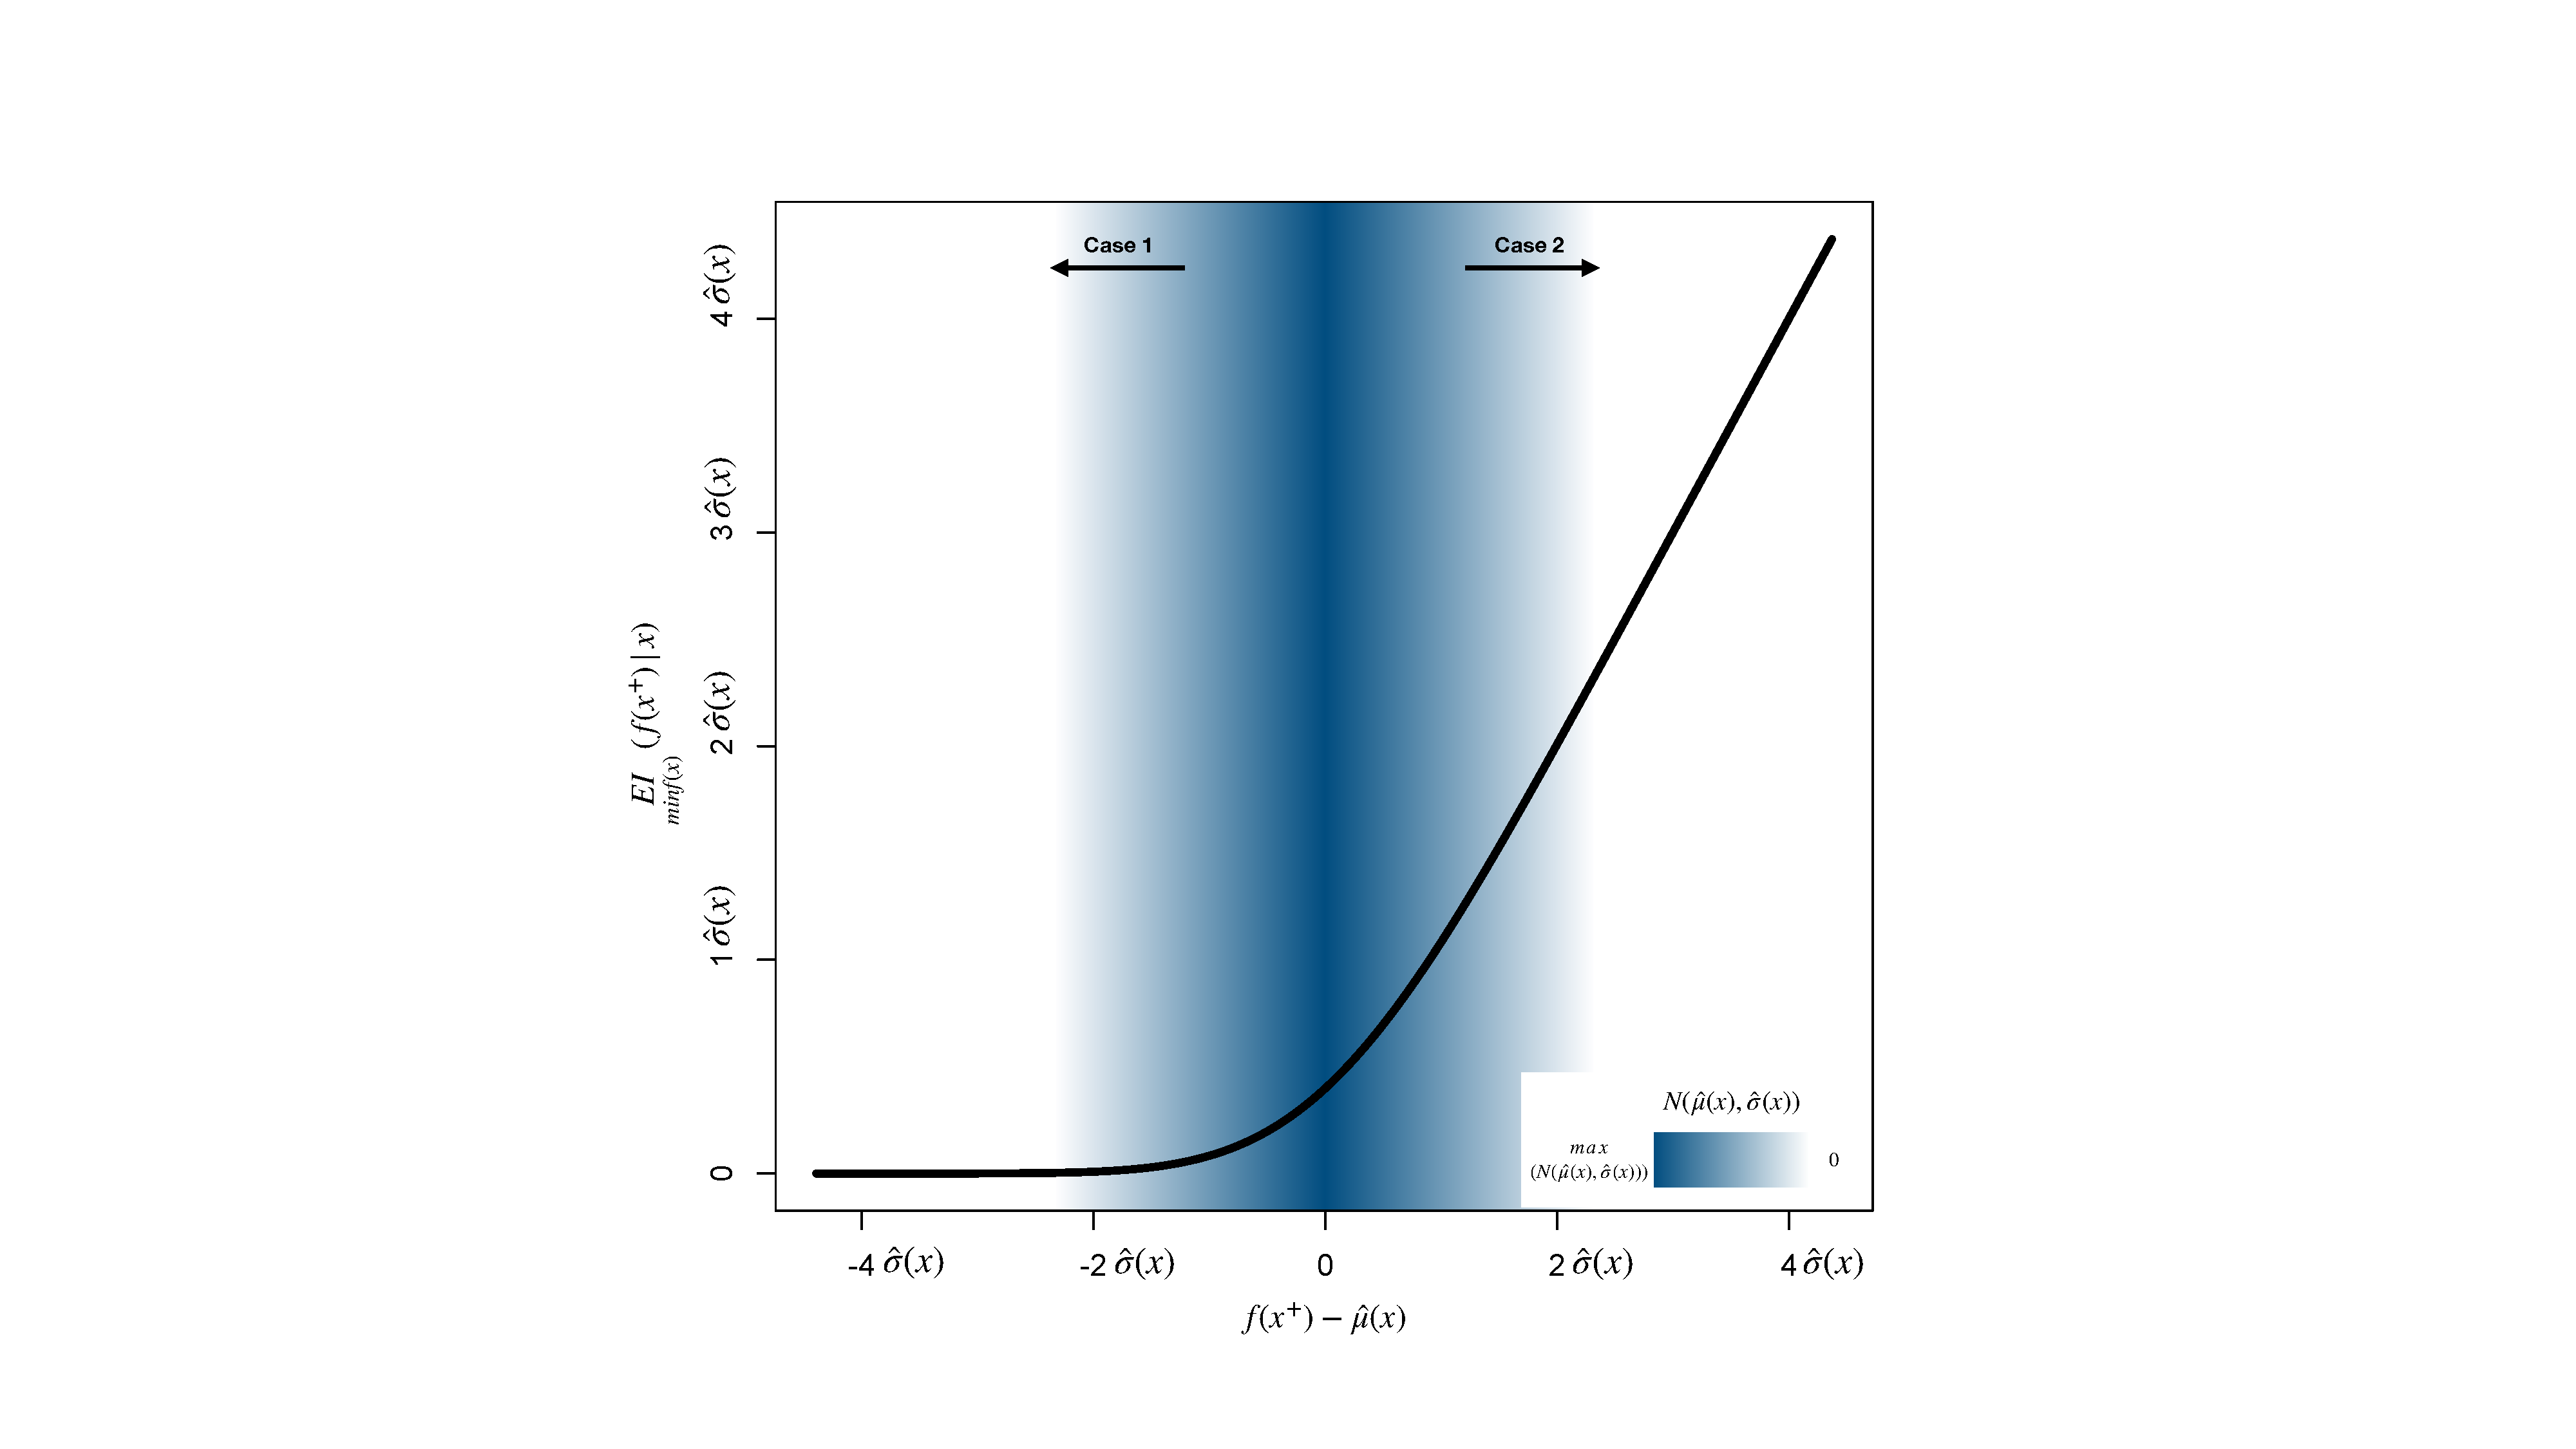
\includegraphics[scale=0.3]{Chapter5/Pictures/Cases_EI.pdf}
    \caption{Variation of $\underset{min f(\bm x)}{EI}(f(\bm x^+)|\bm x)$ for change in reference value $f(\bm x^+)$}
    \label{fig:cases_ei}
\end{figure}

As a first thought, this can be overcome by choosing an appropriate reference value $f_{\mathsf{i}}(\bm x^{\mathsf{i}+})$ depending on the prediction $\hat{f}_{\mathsf{i}}(\bm{x})$. But choosing a reference value $f_{\mathsf{i}}(\bm x^{\mathsf{i}+})$ to define $EI$ depending on where $\hat{f}_{\mathsf{i}}(\bm{x})$ lies in the objective space can make the improvements hard to be compared, since different predictions can have different definition of improvement depending on the choice of the reference value. 
The comparison is also essential for defining NDS for optimization in the context of MOO.
Hence, we augment the $EI$ to have a common frame of reference for comparison, where we consider the axes of the objective space itself as the frame of reference for comparison. The augmentation of $EI$ with $f_{\mathsf{i}}(\bm x^{\mathsf{i}+})$ as reference value is given through the criterion expected value ($EV$)\footnote{We here remind that the expected value can also be otherwise defined as $E(\hat{f}(\bm x))$ in the interval $(-\infty,{f}(\bm x^{++})]$ (detailed in \eqref{EI_cent}) contrary to $EI$ which is defined as $E(f(\bm{x}^{++})-\hat{f}(\bm x))$, but considering $E(\hat{f}(\bm x))$ leads to similar properties as $EI$ in comparing with several reference values} as follows

\begin{equation}
\underset{min f_{\mathsf{i}}(\bm{x})}{EV}(\bm{x}|f_{\mathsf{i}}(\bm x^{\mathsf{i}+})) = f_{\mathsf{i}}(\bm x^{\mathsf{i}+})-\underset{min f_{\mathsf{i}}(\bm{x})}{EI}(\bm{x}| f_{\mathsf{i}}(\bm x^{\mathsf{i}+}))
\label{EV-EI}
\end{equation}

The definition of $EV$ avoids the problem of comparing improvements with several reference values, but the above two cases take a different role for the $EV$ criterion, given as 

\begin{equation}
\begin{array}{l}
\mathbf{Case\,1:}\,
For \,\, \hat{\mu_{\mathsf{i}}}(\bm{x})\pm \hat{\sigma_{\mathsf{i}}}(\bm{x})\gg f_{\mathsf{i}}(\bm x^{\mathsf{i}+}), \, \underset{min f_{\mathsf{i}}(\bm{x})}{EV}(\bm{x}|f_{\mathsf{i}}(\bm x^{\mathsf{i}+}))\approx f_{\mathsf{i}}(\bm x^{\mathsf{i}+})\\
\\
\mathbf{Case\,2:}\,
For \,\, \hat{\mu_{\mathsf{i}}}(\bm{x})\pm \hat{\sigma_{\mathsf{i}}}(\bm{x}) \ll f_{\mathsf{i}}(\bm x^{\mathsf{i}+}), \, \underset{min f_{\mathsf{i}}(\bm{x})}{EV}(\bm{x}|f_{\mathsf{i}}(\bm x^{\mathsf{i}+}))\approx  \hat{\mu_{\mathsf{i}}}(\bm{x})
\end{array}
\end{equation}



For {\textbf{Case 1}}, in the context of $EI$, the improvement becomes infinitesimal or zero for comparison. While in the context of $EV$, this leads to the problem of over-estimation, where the value of $EV$ becomes the reference value itself and hence, an unrealistic reference value can lead to overestimation of improvement. Similarly, the difference in context between $EI$ and $EV$ can be seen for \textbf{Case 2}, where $EV$ simply converges to $\hat{\mu}{(\bm x)}$. This means that two predictions with the same  $\hat{\mu}{(\bm x)}$ but different  $\hat{\sigma_{\mathsf{i}}}(\bm{x})$ will have the same preference. The above cases are graphically shown in Fig. \ref{fig:cases_ev}\\

\begin{figure}[h!]
    \centering
    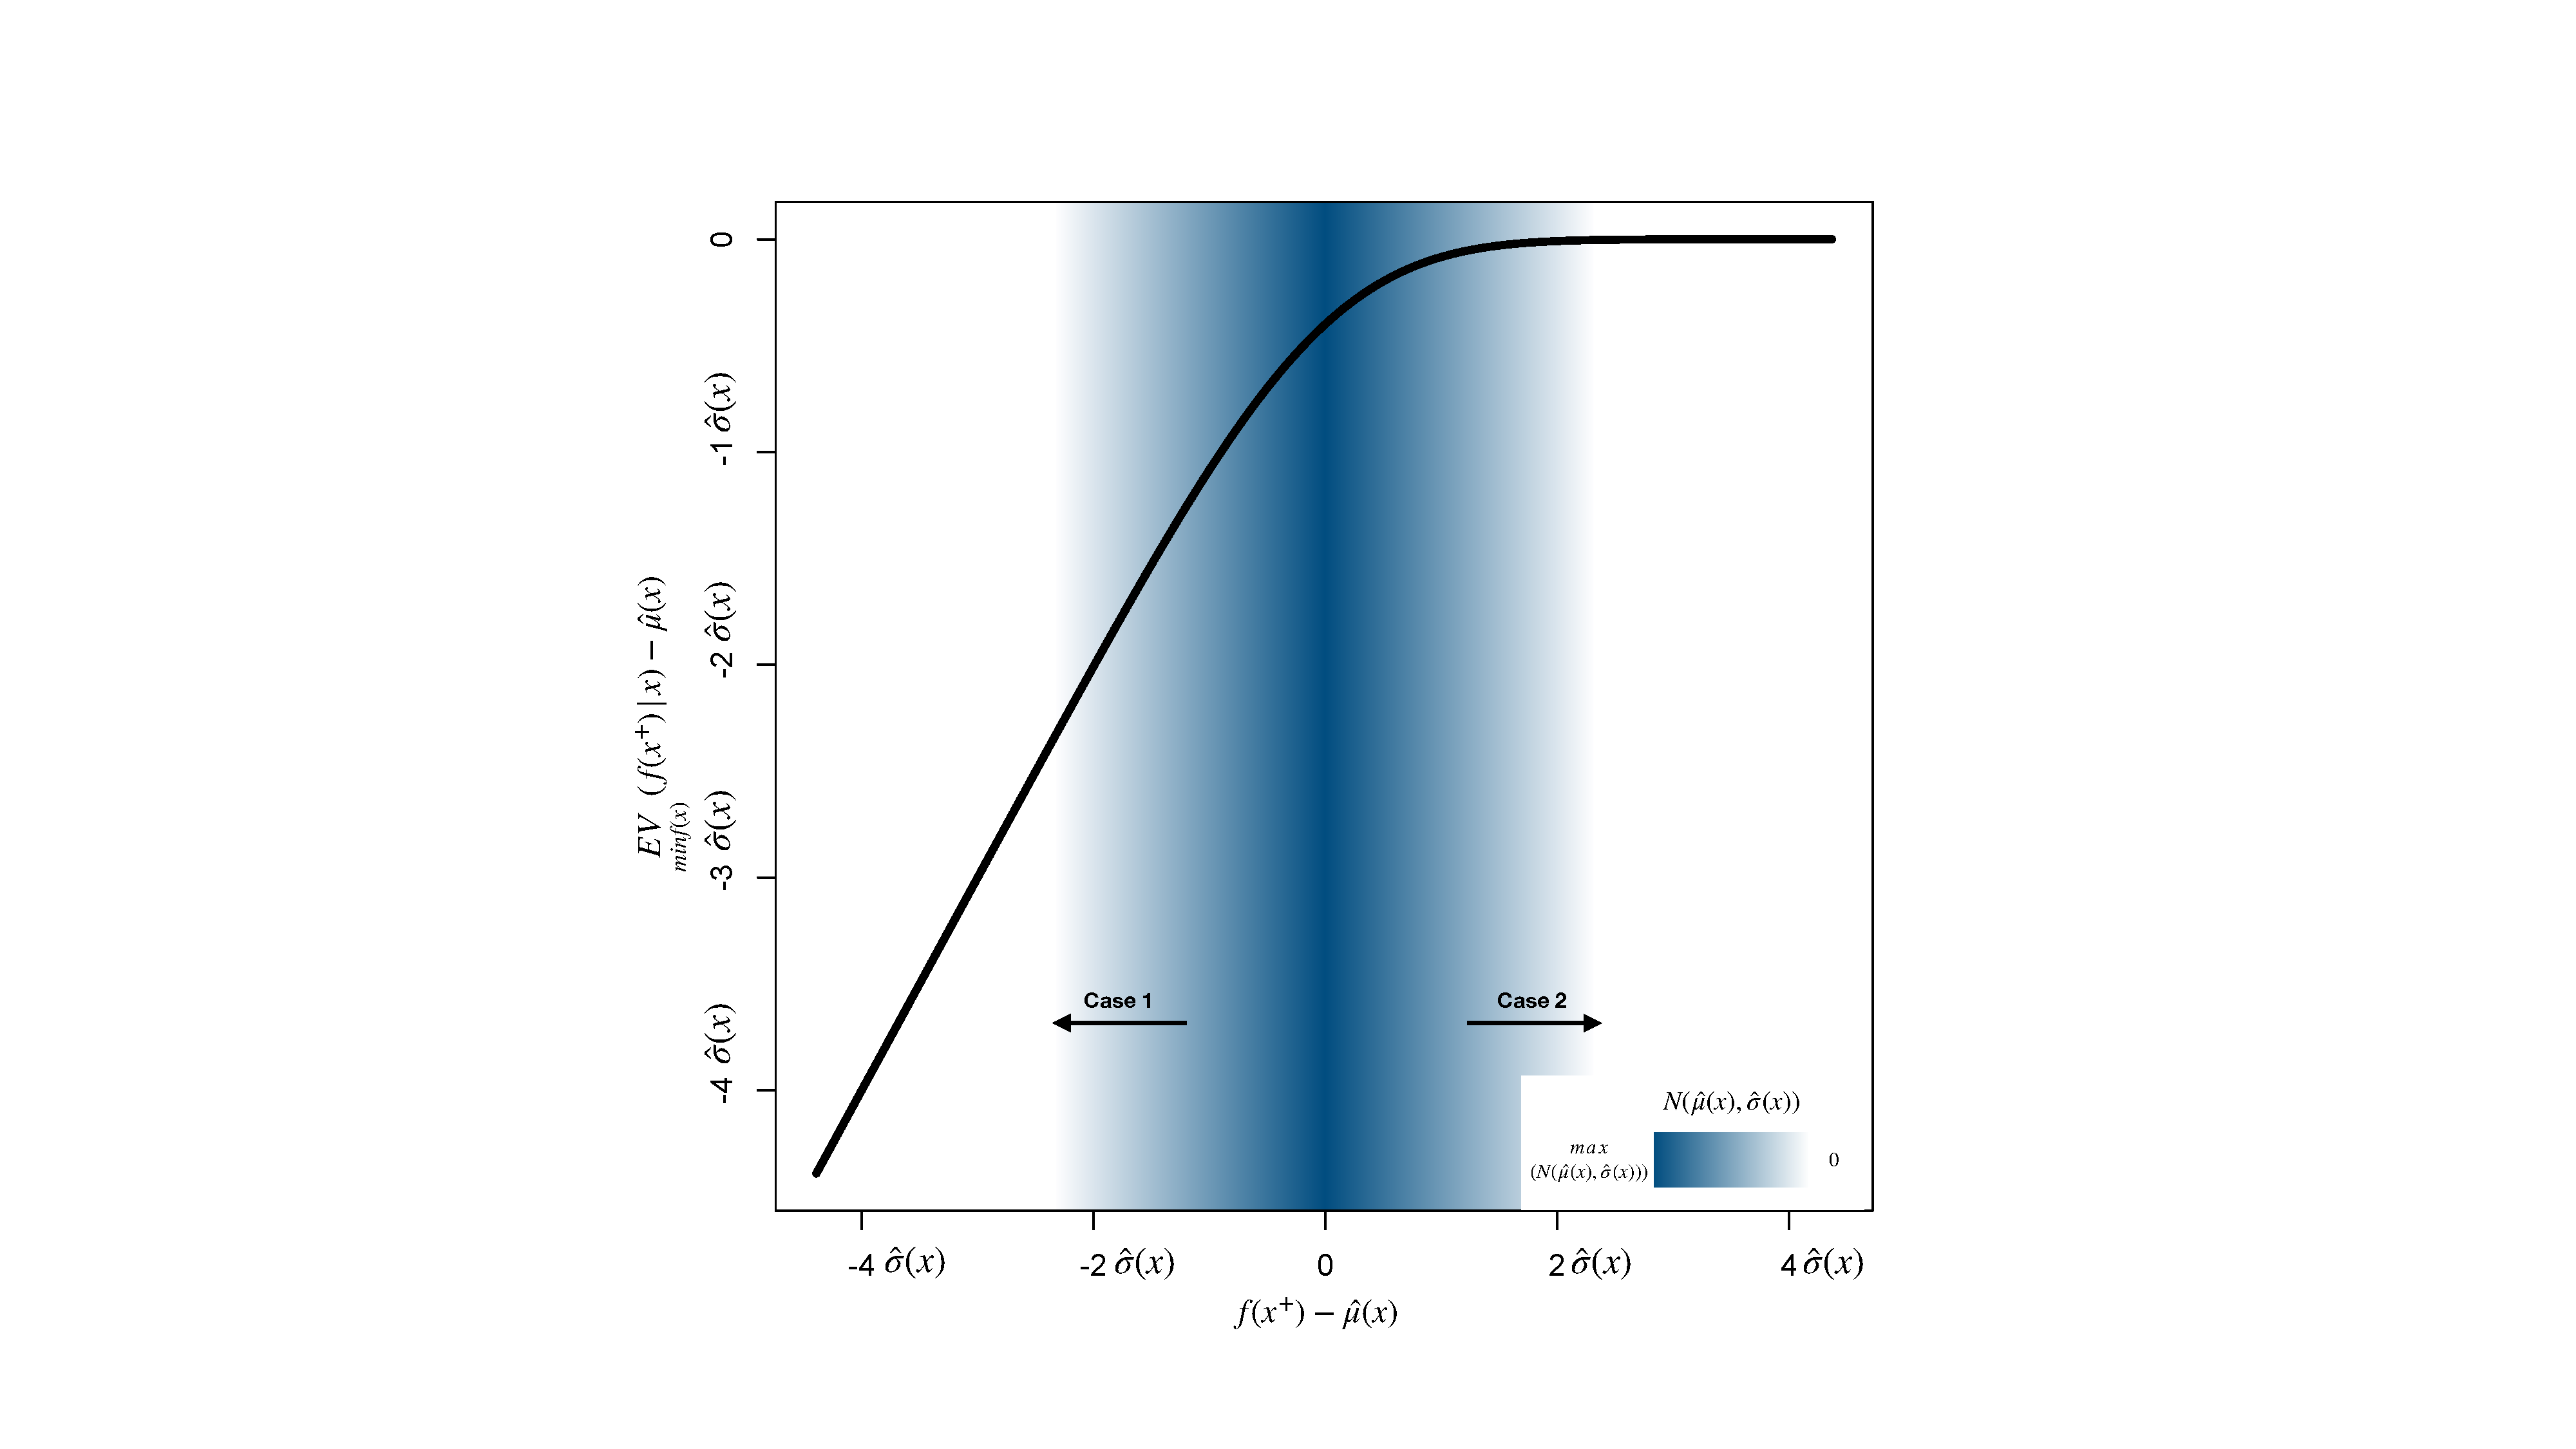
\includegraphics[scale=0.3]{Chapter5/Pictures/Cases_EV.pdf}
    \caption{Variation of $\underset{min f(\bm x)}{EV}(f(\bm x^+)|\bm x)$ for change in reference value $f(\bm x^+)$}
    \label{fig:cases_ev}
\end{figure}

 We give the explanation in avoiding the above cases with $EV$ criterion since it is much easier to work in the coordinates of the objective space. As defined before, \textbf{Case\,1} can be avoided by seeking improvement with respect to a reference value which is more realistic for improvement rather than being too greedy. 
 The realistic scope of improvement considering $f_{\mathsf{i}}(\bm x^{\mathsf{i}+})$ can be defined through the $CDF:$ $\mathcal{P}({f}_{\mathsf{i}}(\bm{x})\leq f_{\mathsf{i}}(\bm x^{\mathsf{i}+}))$ for any $\mathcal{GP}$ outcome $\hat{f}_{\mathsf{i}}(\bm{x}):\mathcal{N}(\hat{\mu_{\mathsf{i}}}(\bm{x}),\hat{\sigma_{\mathsf{i}}}(\bm{x}))$. 
 We here remind that the given $CDF$ is essentially the Probability of Improvement criterion ($PI$). 
 Hence, the $CDF$ constituting to zero for any reference value can be said as being too greedy for improvement, where there can be a limit set for the $CDF$ measure to be considered with compromise on greed. 
 The limit could be set in terms of $\hat{\mu_{\mathsf{i}}}(\bm{x})-\epsilon\hat{\sigma_{\mathsf{i}}}(\bm{x})$\footnote{We give the relation in terms of $LCB$, since for any $f(\bm x^{+}):\mathcal{P}({f}(\bm{x})\leq f(\bm x^{+}))\geq\mathcal{P}({f}(\bm{x})\leq \hat{\mu}(\bm{x})-\epsilon\hat{\sigma}(\bm{x}))$, the following relation holds $f(\bm x^{+}) \geq \hat{\mu}(\bm{x})-\epsilon\hat{\sigma}(\bm{x})$ } where we seek for $\mathcal{P}({f}_{\mathsf{i}}(\bm{x})\leq f_{\mathsf{i}}(\bm x^{\mathsf{i}+}))\geq\mathcal{P}({f}_{\mathsf{i}}(\bm{x})\leq \hat{\mu_{\mathsf{i}}}(\bm{x})-\epsilon\hat{\sigma_{\mathsf{i}}}(\bm{x}))$, with $\epsilon$ being the parameter to be defined. 
 A higher value of $\epsilon$ means higher the greed to seek improvement, but the balance to set the limit could be otherwise seen as the acceptable risk that can be considered for exploration. The higher risk with considering higher value of $\epsilon$ for $\hat{\mu_{\mathsf{i}}}(\bm{x})-\epsilon\hat{\sigma_{\mathsf{i}}}(\bm{x})$ may reap higher benefits but this could be otherwise, since there is equal probability for ${f}_{\mathsf{i}}(\bm{x})\geq\hat{\mu_{\mathsf{i}}}(\bm{x})+\epsilon\hat{\sigma_{\mathsf{i}}}(\bm{x})$. Hence, this requires the right balance for the choice of $\epsilon$ with acceptable risk for exploration.\\

For MOO, the most feasible improvement that we can look for is with respect to the empirical Pareto-front $f_{\mathsf{i}}(\mathscr{P}_{\mathcal{S}}):=\{f_{\mathsf{i}}(\bm{p}_1),f_{\mathsf{i}}(\bm{p}_2),\hdots,f_{\mathsf{i}}(\bm{p}_{(.)})\}$ of the observed samples. But, there can be multiple $\bm{p}_{\mathrm i}:f_{\mathsf i}(\bm{p}_{\mathrm{i}})\leq\hat{\mu_{\mathsf{i}}}(\bm{x})-\epsilon\hat{\sigma_{\mathsf{i}}}(\bm{x})$, where we choose the $\bm{p}_\mathrm{i}$ which gives the minimum value of $\underset{min f_{\mathsf{i}}(\bm{x})}{EV}$. The choice of the minimum value of $\underset{min f_{\mathsf{i}}(\bm{x})}{EV}$ for a function to be minimised averts \textbf{Case\,2} which defines the pessimistic choice of reference value, unless it is not possible when no suitable reference value exists. In overall, the above definitions provide the balance between greed and being pessimistic for improvement through the parameter $\epsilon$. The above definitions could be expressed as follows

\begin{equation} \label{EV_f}
\begin{split}
\underset{min\,f_{\mathsf{i}}(\bm{x})}{EV}(\bm{x}|\mathscr{P}_{\mathcal{S}},\epsilon) &= \underset{\bm{p}_{\mathrm i}\in \mathscr{P}_s}{min}(\underset{min f_{\mathsf{i}}(\bm{x})}{EV}(f_{\mathsf{i}}(\bm{p}_{\mathrm{i}})|\bm{x})) \\
\mathscr{P}_s &:=\{  f_{\mathsf{i}}(\bm{p}_{\mathrm i})\geq\hat{\mu_{\mathsf{i}}}(\bm{x})-\epsilon\hat{\sigma_{\mathsf{i}}}(\bm{x}),\forall\bm{p}_{\mathrm i}\in\mathscr{P}_{\mathcal{S}}\}
\end{split}
\end{equation}

where the discrete optimisation of $\underset{\bm{p}_{\mathrm i}\in \mathscr{P}_s}{min}(\underset{min f_{\mathsf{i}}(\bm{x})}{EV}(f_{\mathsf{i}}(\bm{p}_{\mathrm i})|\bm{x}))$ can be implicitly satisfied through defining NDS with $\underset{min\,f_{\mathsf{i}}(\bm{x})}{EV}(\bm{x}|\mathscr{P}_{\mathcal{S}},\epsilon)$. 
Alternatively, from the nature of proportionality for $\underset{min f_{\mathsf{i}}(\bm{x})}{EV}(f_{\mathsf{i}}(\bm{p}_{\mathrm{i}})|\bm{x})) \propto f_{\mathsf{i}}(\bm{p}_{\mathrm i})$, shown in Fig. \ref{fig:cases_ev}, the most suitable reference value $f_{\mathsf{i}}(\bm{p}_{\mathrm i}^\star)$ to achieve $\underset{\bm{p}_{\mathrm i} \in \mathscr{P}_s}{min}(\underset{min f_{\mathsf{i}}(\bm{x})}{EV}(f_{\mathsf{i}}(\bm{p}_{\mathrm i})|\bm{x}))$ can be simply given as  $f(\bm{p}_{\mathrm i}^\star)=\underset{\bm{p}_{\mathrm i}\in \mathscr{P}_s}{min} f(\bm{p}_{\mathrm i})$.  In short, we define the Eq. \eqref{EV_f} as $EV$ criterion for the following discussions.\\

The given definitions allow to define $EV$ criterion in the place of $EI$, where the problem \eqref{Optim_EIs} can be redefined as follows

 \begin{equation}\label{Optim_EVs}
 \underset{\bm x \in \mathcal{X}}{min}\Big[ \underset{min\,f_1(\bm{x})}{EV}(\bm{x}|\mathscr{P}_{\mathcal{S}},\epsilon) \cdots \underset{min\,f_{\mathsf{m}}(\bm{x})}{EV}(\bm{x}|\mathscr{P}_{\mathcal{S}},\epsilon)  \Big]
 \end{equation}
 
 The MOO can be achieved through NSGA-2, which leads to Pareto-optimal solutions $(\mathscr{P}_{\hat{\mathcal{S}}})$. The independent definition of improvement allows to work with only univariate Gaussian distributions and hence, large number of $EV$ criteria could be optimised with relatively ease.\\
 
 The primary goal for choosing $f_{\mathsf{i}}(\bm{p}_{\mathrm i}) \in f_{\mathsf{i}}(\mathscr{P}_{\mathcal{S}})$ independently for each $\underset{min\,f_{\mathsf{i}}(\bm{x})}{EV}(\bm{x}|\mathscr{P}_{\mathcal{S}},\epsilon)$ is that it can lead to choosing reference points $\bm f(\bm{p}_{\mathrm i}) \in \bm f(\mathscr{P}_{\mathcal{S}})$, where the intention is to define improvements $\mathfrak{I}_{\bm f(\bm{p}_{\mathrm i})}$ 
 %\footnote{$\mathscr{I}_{\bm{f}^*} (\bm x) =\Big[\underset{min\,f_1(\bm{x})}{EV}(\bm x|f^*_1) \cdots \underset{min\,f_{\mathsf{m}}(\bm{x})}{EV}(\bm x|f^*_{\mathsf{m}})\Big]$, {\bm{f}^* =[f^*_1 \cdots f^*_{\mathsf{m}}]} }
  \footnote{$\mathscr{I}_{\bm{f}^*} (\bm x)$ $\in \mathfrak{I}_{\bm{f}^*}=$$\Big\{\Big[\underset{min\,f_1(\bm{x})}{EV}(\bm x|f^*_1) \cdots \underset{min\,f_{\mathsf{m}}(\bm{x})}{EV}(\bm x|f^*_{\mathsf{m}})\Big]| \forall \mathsf{i},f_{\mathsf{i}}^{*} = \underset{\bm{p}_{\mathrm i}\in \mathscr{P}_s}{min} f_{\mathsf{i}}(\bm{p}_{\mathrm i}), \forall \bm x \in \mathcal{X}\Big\}$, ${\bm{f}^* =[f^*_1 \cdots f^*_{\mathsf{m}}]}$} (Fig. \ref{fig:improv_illus}). %where $\mathfrak{I}_{\bm{f}^*}$ is the set of all possible improvements with respect to the reference point $\bm{f}^*$} that can dominate $\bm f(\bm{p}_{\mathrm i}) \in  \bm f(\mathscr{P}_{\mathcal{S}})$.
 The choice of $f_{\mathsf{i}}(\bm{p}_{\mathrm i})$ independently for each $\underset{min\,f_{\mathsf{i}}(\bm{x})}{EV}(\bm{x}|\mathscr{P}_{\mathcal{S}},\epsilon)$ means that it can implicitly lead to choosing reference points $[\bm g_{\mathsf 1}= f_{\mathsf{1}}(\bm{p}_{\mathrm i}) \in f_{\mathsf{1}}(\mathscr{P}_{\mathcal{S}}), \cdots, \bm g_{\mathsf m}= f_{\mathsf{m}}(\bm{p}_{\mathrm i}) \in f_{\mathsf{m}}(\mathscr{P}_{\mathcal{S}}) ]$\footnote{It should be noted that the choice of $\bm{p}_{\mathrm i}$ is independent for each $f_{\mathsf{i}}$}$\in \mathbb{R}^{\mathsf{m}}$ from a grid of points $\mathscr{G}:=\{f_{\mathsf{1}}(\mathscr{P}_{\mathcal{S}}) \times \cdots  \times f_{\mathsf{m}}(\mathscr{P}_{\mathcal{S}})\}$. 
This means that $\bm f(\mathscr{P}_{\mathcal{S}})\subset\mathscr{G}$, where $\mathscr{G}$ also contains points which dominate or be dominated by points in the set $\bm f(\mathscr{P}_{\mathcal{S}})$, which includes the Utopian point: $\bm g_{\mathsf{o}} \preceq \bm f(\mathscr{P}_{\mathcal{S}})$ \footnote{$\bm g_{\mathsf o} $ is an arbitrary point in $\mathscr{G}$ with index $\mathsf{o}$} and the Nadir point: $\forall {\mathrm{i}}, \bm f(\bm p_{\mathrm{i}})  \preceq {\bm g_{\mathsf{o}}}$.  
  \iffalse
  This means that any improvement $ \mathscr{I}_{\bm {g}_{\mathsf o}}$ defined with a reference point $\bm {g}_{\mathsf j} \in \mathscr{G}$ falls in to one of the categories, 
  
  \begin{itemize}
  \item if $\bm g_{\mathsf{o}} \in \bm f(\mathscr{P})$, then $\mathscr{I}_{f_{\mathsf{i}}(\bm{p}_{\mathrm i})}$ can be said to dominate a point $\bm f(\bm p_{\mathrm{i}})$ in the Pareto-front,  where $\bm f(\bm p_{\mathrm{i}}) = \bm g_{\mathsf{j}}$
  \item if $\bm g_{\mathsf{j}} \preceq \bm f(\bm p_{\mathrm{i}})$, then any improvement defined with $\bm g_{\mathsf{j}}$ also dominates $f(\bm p_{\mathrm{i}})$ 
   \item if $\bm f(\bm p_{\mathrm{i}}) \preceq \bm g_{\mathsf{j}}$

  \end{itemize}
  \fi
  This means that improvements can not only be defined to dominate any empirical Pareto-front point $\bm f({\bm{p}_{\mathrm{i}}}) \in \bm f  (\mathscr{P}_{\mathcal{S}})$, but also multiple Pareto-front points in the set $\bm f(\mathscr{P}_{\mathcal{S}})$.\\
  
  \begin{figure}
     \centering
    \includegraphics[scale=0.35]{Chapter5/Pictures/improv_illus}
    \caption{Illustration of the set $\mathfrak{I}_{\bm f(\bm{p}_{\mathrm i})}$ and its associated subsets}
    \label{fig:improv_illus}
 \end{figure}
  
 With the population based evolutionary strategy of NSGA-2, for a given population, the optimisation is simultaneously defined with several reference points in the objective space. This means that the individuals in a given generation of NSGA-2 are defined with their respective reference point and since the improvements are represented as expected values in the objective space, comparisons can be made to define non-dominated sorting and niching operations. This implicitly models optimisation of several $EI$s in the objective space, with each $EI$ defined with a unique reference point, illustrated in \ref{fig:EV_EIss}. \\
  
  
 
 
  %Though, a reference value $f_{\mathsf{i}}(\bm{p}_{\mathrm i}) \in f_{\mathsf{i}}(\mathscr{P}_{\mathcal{S}})$ is chosen independently for each $\underset{min\,f_{\mathsf{i}}(\bm{x})}{EV}(\bm{x}|\mathscr{P}_{\mathcal{S}},\epsilon)$, this implicitly leads to choosing a reference point $[f_{\mathsf{1}}(\bm{p}_{\mathrm i}) \in f_{\mathsf{1}}(\mathscr{P}_{\mathcal{S}}), \cdots, f_{\mathsf{m}}(\bm{p}_{\mathrm i}) \in f_{\mathsf{m}}(\mathscr{P}_{\mathcal{S}}) ]$\footnote{It should be noted that the choice of $\bm{p}_{\mathrm i}$ is independent for each $f_{\mathsf{i}}$}$\in \mathbb{R}^{\mathsf{m}}$from a grid of points $\{f_{\mathsf{1}}(\mathscr{P}_{\mathcal{S}}) \times f_{\mathsf{2}}(\mathscr{P}_{\mathcal{S}})  \times \cdots  \times f_{\mathsf{m}}(\mathscr{P}_{\mathcal{S}})\}$ for any prediction $\bm{\hat{f}}(\bm x)$. 
  %For $\mathsf{n}_{\mathscr{P}_{{\mathcal{S}}}}$ number of points in $\mathscr{P}_{\mathcal{S}}$, number of grid points scale by  ${(\mathsf{n}_{\mathscr{P}_{{\mathcal{S}}}}})^\mathsf{m}$. This can be seen as improvement being defined independently with each reference point in $\mathbb{R}^{\mathsf{m}}$, where the improvement defines the dominance in $\mathbb{R}^{\mathsf{m}}$ over its respective reference point.
 %Hence, the optimisation of the improvement is also simultaneously defined with several reference points in the objective space. This means that the individuals in a given generation of NSGA-2 are defined with their respective reference point and since the improvements are represented as the expected values in the objective space, comparisons can be made to define non-dominated sorting and niching operations.\\
 
 \begin{figure}
     \centering
    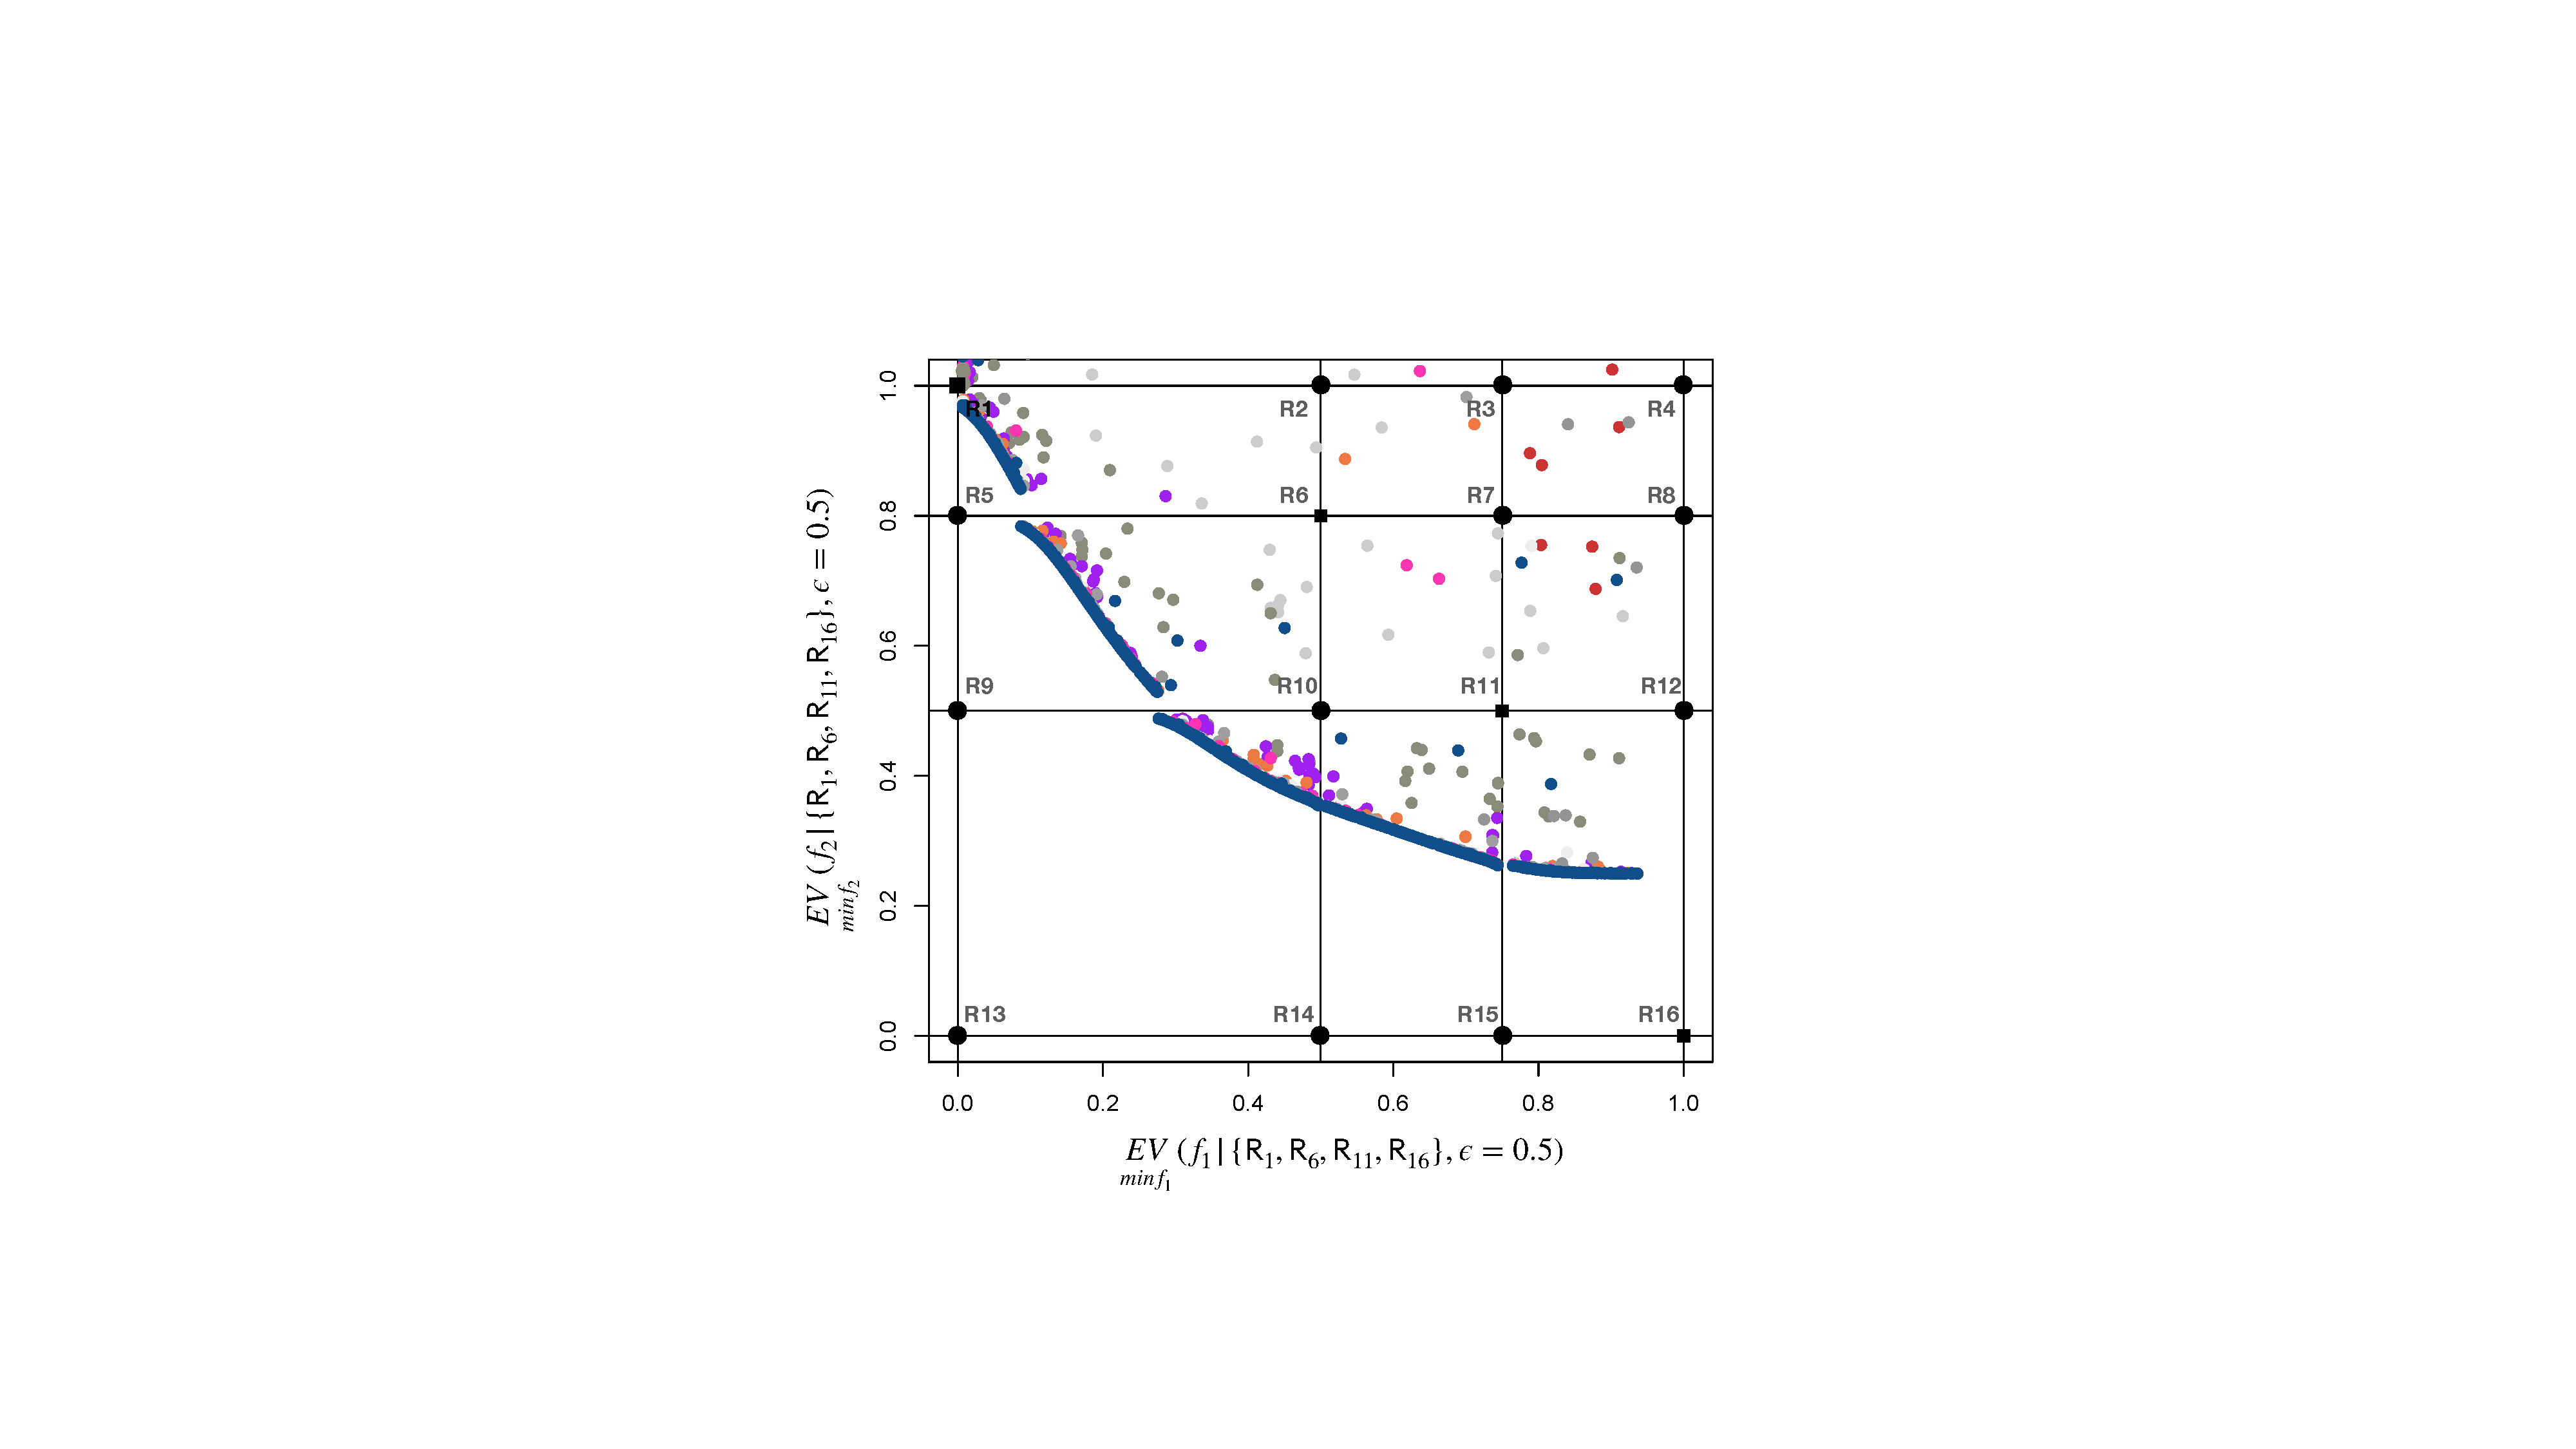
\includegraphics[scale=0.4]{Chapter5/Pictures/EV_ZDT1.pdf}
    \caption{An example for optimization of EV}
    \label{fig:eg:EV}
 \end{figure}
 
 An example for the optimisation of \eqref{Optim_EVs} is shown in Fig. , for a simple MOO test functions set: ZDT1 of two dimensions $(\mathsf{m}=2)$. 
 In this case, $\bm f(\mathscr{P}_{\mathcal{S}})=\{\bm{\mathsf{R}}_1, \bm{\mathsf{R}}_6, \bm{\mathsf{R}}_{11}, \bm{\mathsf{R}}_{16}\}$, $\mathscr{G}=\{\bm{\mathsf{R}}_1,\cdots,\bm{\mathsf{R}}_{16}\}$.
The Pareto front  $\bm f(\mathscr{P}_{\hat{\mathcal{S}}})$ is defined by the reference points $\bm{\mathsf{R}}_{2},\bm{\mathsf{R}}_{6},\bm{\mathsf{R}}_{10},\bm{\mathsf{R}}_{11},\bm{\mathsf{R}}_{16}$, where two of the reference points $\bm{\mathsf{R}}_6$ and $\bm{\mathsf{R}}_{11}$ belong to $\mathscr{P}_{\mathcal{S}}$. This means that the improvements $\mathfrak{I}_{\bm{\mathsf{R}}_6}$ and $\mathfrak{I}_{\bm{\mathsf{R}}_{11}}$ independently define domination over $\bm{\mathsf{R}}_6$ and $\bm{\mathsf{R}}_{11}$ respectively, as $\mathfrak{I}_{\bm{\mathsf{R}}_6} \preceq \bm{\mathsf{R}}_6$ and $\mathfrak{I}_{\bm{\mathsf{R}}_{11}} \preceq \bm{\mathsf{R}}_{11}$.
For $\bm{\mathsf{R}}_{10}$, something interesting happens, where $\bm{\mathsf{R}}_{10} \notin \mathscr{P}_{\mathcal{S}}$ but is purely an outcome of the implicit definition of grid $\mathscr{G}$. In this case, $\bm{\mathsf{R}}_{10} \preceq \{\bm{\mathsf{R}}_6$,  $\bm{\mathsf{R}}_{11}\}$, hence also the improvements $\mathfrak{I}_{\bm{\mathsf{R}}_{10}} \preceq \{\bm{\mathsf{R}}_6$,  $\bm{\mathsf{R}}_{11}\}$, i.e., any improvement $\mathscr{I}_{\bm{\mathsf{R}}_{10}} \in \mathfrak{I}_{\bm{\mathsf{R}}_{10}}$ dominates the two Pareto-front points $\bm{\mathsf{R}}_6$ and $\bm{\mathsf{R}}_{11}$. 
Hence, $\mathscr{G}$ consists of reference points to define improvements with respect to any $\bm f (\bm p_{\mathrm i})$ or combination of several $\bm f (\bm p_{\mathrm i})$. $\mathscr{G}$ also contains points $\bm g_{\mathsf{o}}: \bm f(\mathscr{P}_{\mathcal{S}})\preceq \bm g_{\mathsf{o}}$ where the improvements defined with such points are essential for guiding the solutions to define $\mathscr{P}_{\hat{\mathcal{S}}}$. The reference points $\bm{\mathsf{R}}_2$ and $\bm{\mathsf{R}}_{12}$ are also weakly dominated by the points in the set $\bm f(\mathscr{P}_{\mathcal{S}})$, where in this case, the improvements $\mathfrak{I}_{\bm{\mathsf{R}}_2}$ are presumed to define the intermediate points between ${\bm{\mathsf{R}}_1}$ and ${\bm{\mathsf{R}}_6}$, and similarly the improvements $\mathfrak{I}_{\bm{\mathsf{R}}_{12}}$ are presumed to define the intermediate points between ${\bm{\mathsf{R}}_{11}}$ and ${\bm{\mathsf{R}}_{16}}$.
In this example, the Utopian point corresponds to ${\bm{\mathsf{R}}_{12}} \preceq \bm f(\mathscr{P}_{\mathcal{S}})$ and the Nadir point corresponds to  ${\bm{\mathsf{R}}_4}$ where all the points in $\mathscr{G}$ except ${\bm{\mathsf{R}}_4}$ dominates ${\bm{\mathsf{R}}_4}$. \\


 \begin{figure}
     \centering
    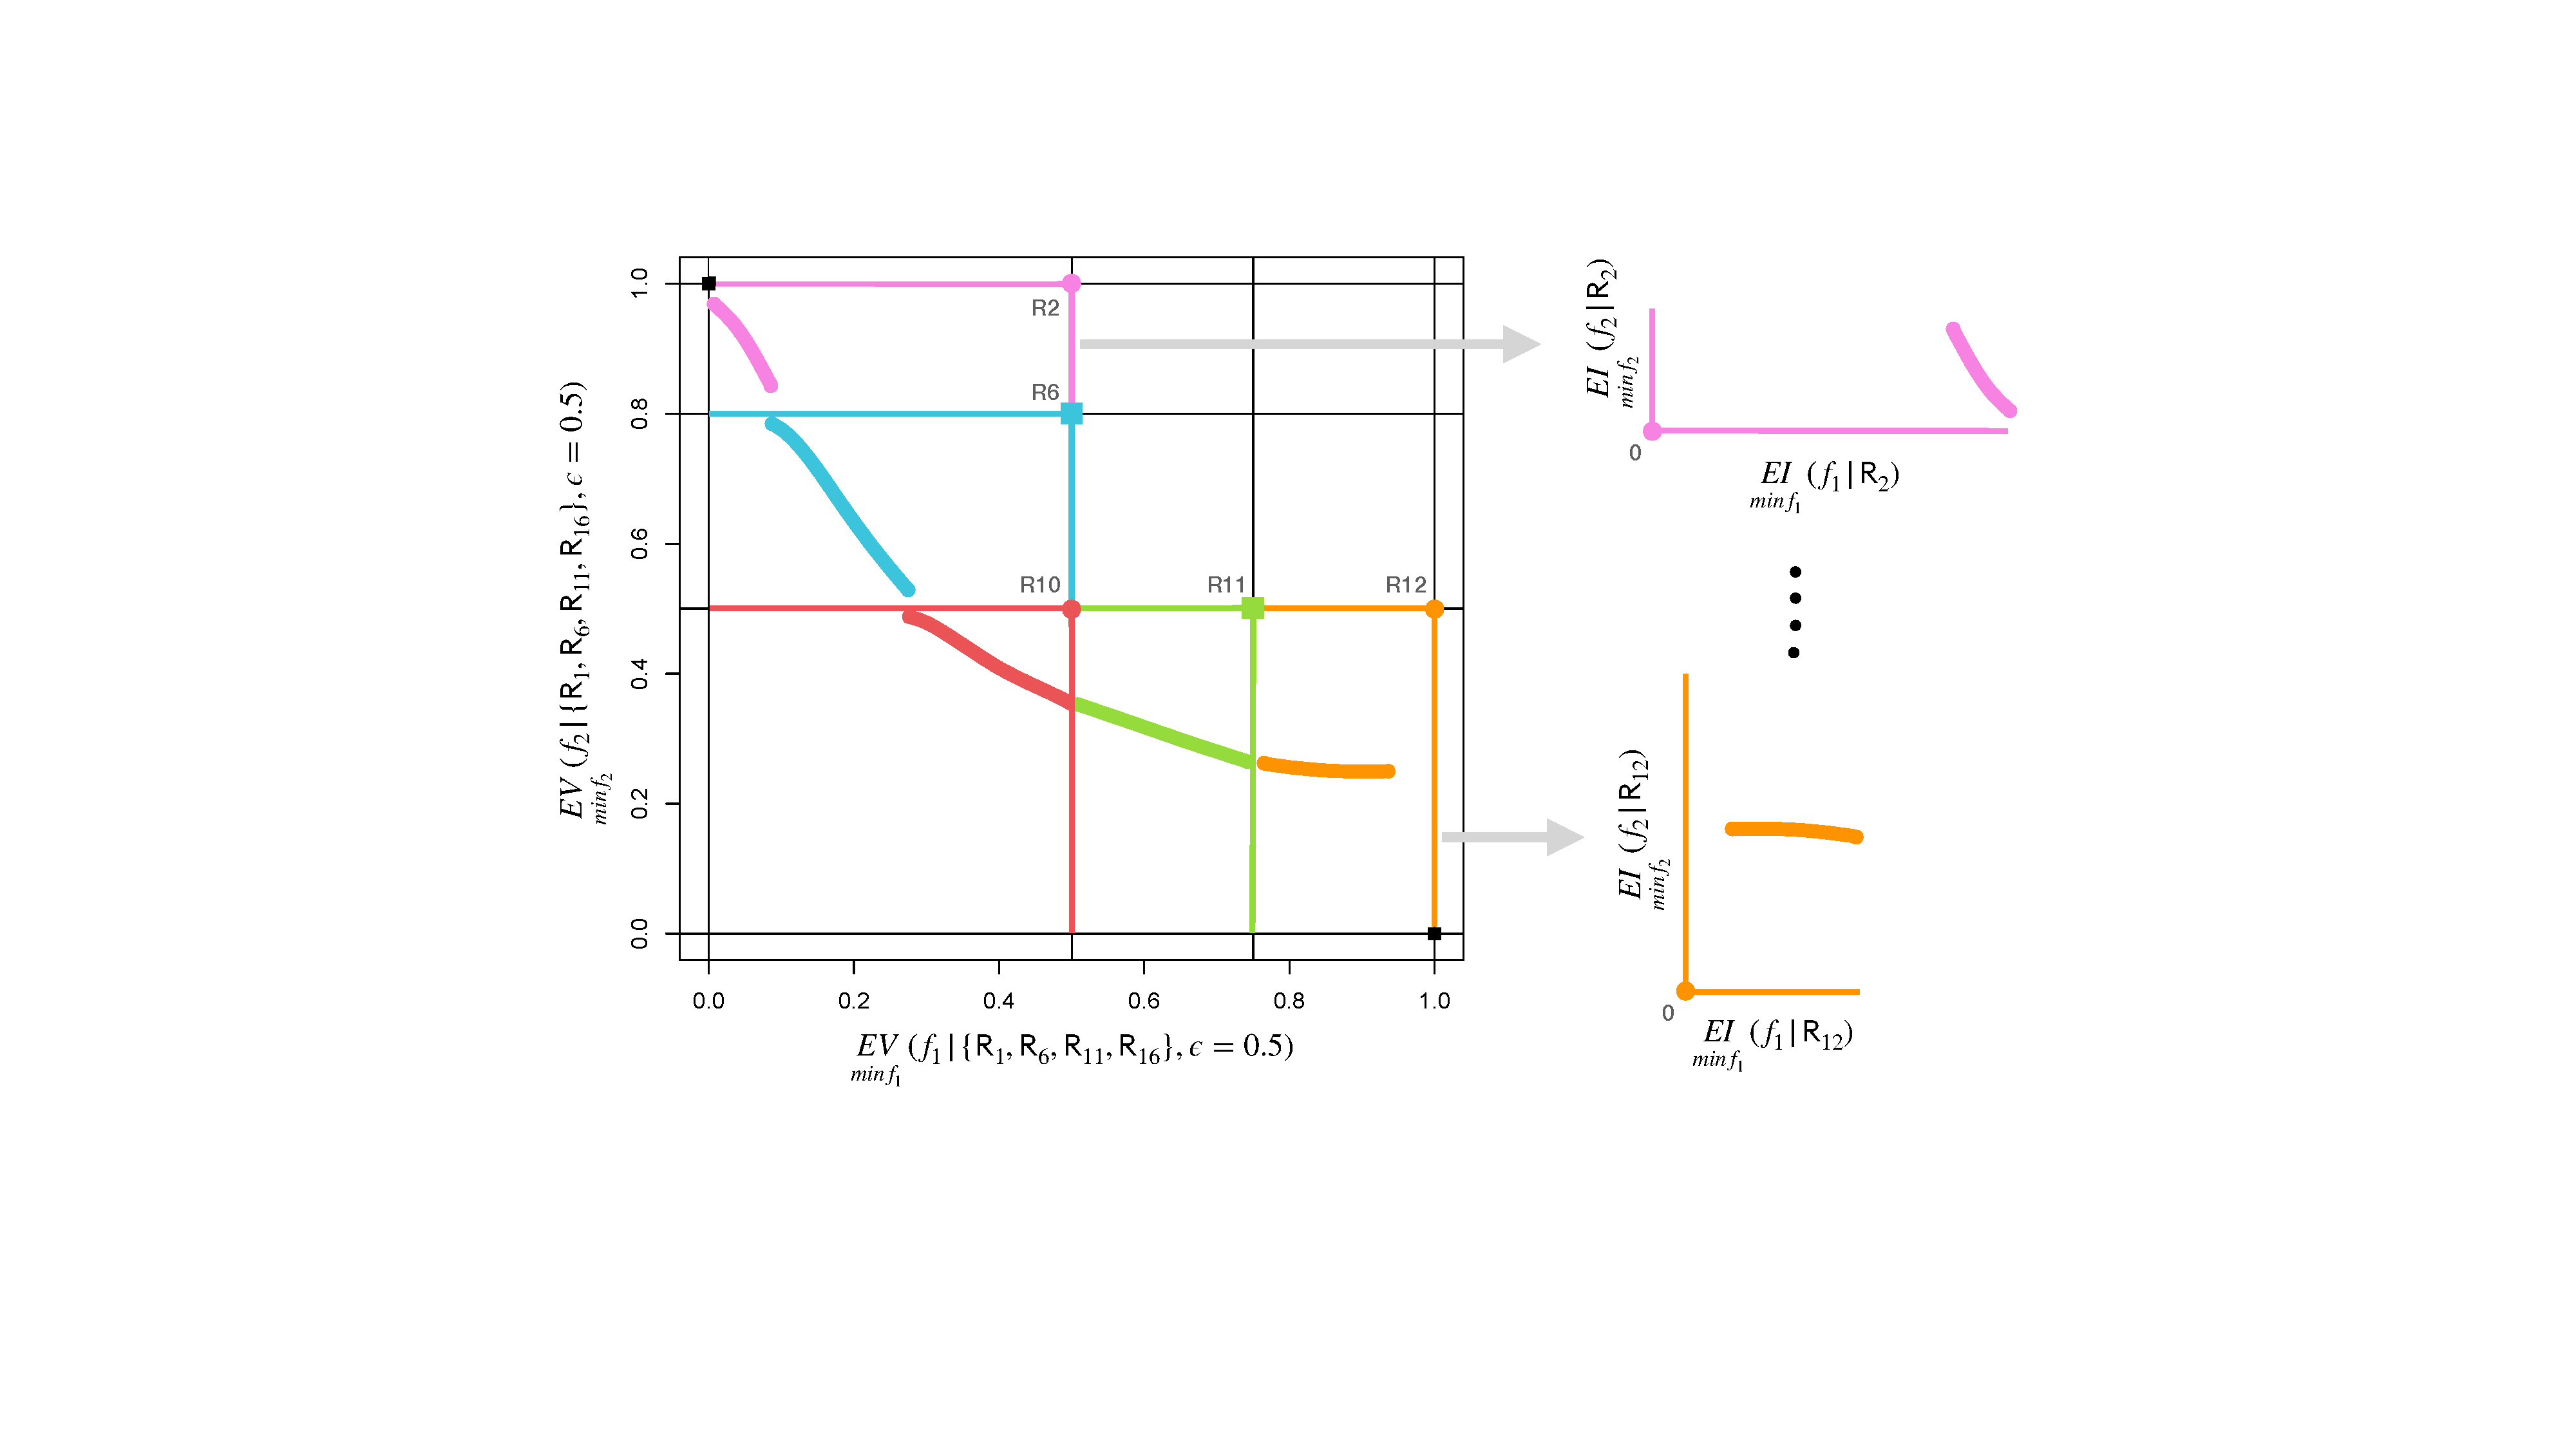
\includegraphics[scale=0.4]{Chapter5/Pictures/EV_rel_EI_ZDT1.pdf}
    \caption{Relation of $EV$ to reference point}
    \label{fig:EV_EIss}
 \end{figure}
 
 
 

Once $\mathscr{P}_{\hat{\mathcal{S}}}$ is obtained optimising Eq. \eqref{Optim_EVs} with NSGA-2, the problem leads to choosing the infill points among  $\mathscr{P}_{\hat{\mathcal{S}}}$. 
Firstly, we discuss the preference of choosing an improvement $\mathscr{I}_{\bm f^*} \in \mathfrak{I}_{\bm f^*}$, where the reference point ${\bm f^*}$ can be considered to define a part of $\bm f(\mathscr{P}_{\hat{\mathcal{S}}})$, i.e., $\{ \mathfrak{I}_{\bm f^*} \cap\bm f(\mathscr{P}_{\hat{\mathcal{S}}})\} \neq \emptyset$.
The part of the Pareto-front defined by ${\bm f^*}$ can hence be expressed as $\mathscr{P}_{\hat{\mathcal{S}}}^{\bm f^*} = \{ \mathfrak{I}_{\bm f^*} \cap \bm f(\mathscr{P}_{\hat{\mathcal{S}}})\}$, where the choice of an infill point in the set  $\mathfrak{I}_{\bm f^*}$ can be narrowed down to choosing a point  $\mathscr{I}_{\bm f^*} \in \bm f(\mathscr{P}_{\hat{\mathcal{S}}}^{\bm f^*})$. A suitable measure to quantify $\mathscr{I}_{\bm f^*}$ with respect to ${\bm f^*}$ can be given through hypervolume metric as

\begin{equation}\label{HVI_ref}
HVI(\mathscr{I}_{\bm f^*}|{\bm f^*})=\prod_{\mathsf{i}=1}^{\mathsf{m}} f_{\mathsf{i}}^*-\underset{min\,f_{\mathsf i}(\bm{x})}{EV}(\bm x|f^*_i)
\end{equation}

Hence, the most suitable choice of $\mathscr{I}_{\bm f^*} \in \bm f ( \mathscr{P}_{\hat{\mathcal{S}}}^{\bm f^*})$ is which maximises  $HVI(\mathscr{I}_{\bm f^*}|{\bm f^*})$, expressed as $\underset{\mathscr{I}_{\bm f^*} \in \bm f(\mathscr{P}_{\hat{\mathcal{S}}}^{\bm f^*})}{max} HVI(\mathscr{I}_{\bm f^*}|{\bm f^*})$.  It should be noted that, in this case, $HVI(\mathscr{I}_{\bm f^*}|{\bm f^*})$ is equivalent to ${EHVI}(\bm{x}|{\bm f^*})$, which is also similar to the criteria $mEI$ detailed in $\label{mEI}$, since $ f_{\mathsf{i}}^*-\underset{min\,f_{\mathsf i}(\bm{x})}{EV}(\bm x|f^*_i)=\underset{min\,f_{\mathsf i}(\bm{x})}{EI}(\bm x|f^*_i)$. The calculation of $HVI$ in this case is analytical and simple irrespective of the dimensions.\\

The choice of $\underset{\mathscr{I}_{\bm f^*} \in \bm f(\mathscr{P}_{\hat{\mathcal{S}}}^{\bm f^*})}{max} HVI(\mathscr{I}_{\bm f^*}|{\bm f^*})$ essentially expresses the best $HVI$ with respect to $\bm f^*$, but it makes no relation of $HVI$ relative to $\bm f(\mathscr{P}_{\mathcal S})$. 
While $HVI$ relative to $\bm f(\mathscr{P}_{\mathcal S})$ can simply be expressed as ${HVI}(\mathscr{I} |\bm f(\mathscr{P}_{\mathcal{S}}), \bm{\mathsf{R}})$\footnote{$\mathscr{I}$ is an arbitrary improvement point where we do not focus on the reference point with which it is defined, contrary to $\mathscr{I}_{\bm f^*}$}, this is quite an expensive strategy to pick an infill point from $\mathscr{P}_{\hat{\mathcal{S}}}$, since this requires evaluation of ${HVI}(\mathscr{I} |\bm f(\mathscr{P}_{\mathcal{S}}), \bm{\mathsf{R}})$ for all $\mathscr{I} \in  \mathscr{P}_{\hat{\mathcal{S}}}$. Since $HVI$ with respect to $\bm f^*$ is known, it can be said that the relation of $\mathscr{I}_{\bm f^*}$  with respect to $\mathscr{P}_{\hat{\mathcal{S}}}$ can be defined by counting the ${HVI}({\bm f^*} |\bm f(\mathscr{P}_{\mathcal{S}}), \bm{\mathsf{R}})$, expressed as

\begin{equation}
HVI_{\uplus}(\mathscr{I}_{\bm f^*}|\bm f(\mathscr{P}_{\mathcal{S}}), \bm{\mathsf{R}})=HVI(\mathscr{I}_{\bm f^*}|{\bm f^*})+
{HVI}({\bm f^*} |\bm f(\mathscr{P}_{\mathcal{S}}), \bm{\mathsf{R}})
\end{equation} 

The idea is that instead of defining ${HVI}(\mathscr{I} |\bm f(\mathscr{P}_{\mathcal{S}}), \bm{\mathsf{R}})$ for all $\mathscr{I} \in  \mathscr{P}_{\hat{\mathcal{S}}}$, the computation of  higher complexity $HVI((.)|\bm f(\mathscr{P}_{\mathcal{S}}), \bm{\mathsf{R}})$ is limited to the reference points $\bm g_o \in \mathscr{G}$ for which $\{ \mathfrak{I}_{\bm g_o} \cap \mathscr{P}_{\hat{\mathcal{S}}}\} \neq \emptyset$. With the definition of $HVI((.)|\bm f(\mathscr{P}_{\mathcal{S}}), \bm{\mathsf{R}})$ for a $\bm g_o$, the definition of $HVI$ for any improvement  
$\mathscr{I}_{\bm f^*} \in \mathfrak{I}_{\bm f^*}$ is given by simple product relation in \eqref{HVI_ref}. The infill point from ${\mathscr P}_{\hat{\mathcal S}}$ to define the maximum $HVI$ relative to $\mathscr P_{\mathcal S}$ can be expressed as

\begin{equation}
\bm x^{\iota}= \underset{\bm x \in \mathcal{X}}{arg\, max} \Big\{ HVI_{\uplus}(\mathscr{I}_{\bm g_o}(\bm x)|\bm f(\mathscr{P}_{\mathcal{S}}),\bm{\mathsf{R}})|  \{\mathfrak{I}_{\bm g_o}\cap \bm f(\mathscr{P}_{\hat{\mathcal S}})\} \neq \emptyset, \forall \bm g_o \in\mathscr{G},\forall \bm x \in \mathcal{X} \Big\}
\end{equation} 

Essentially, we scalarise $\mathscr{I} \in \mathscr{P}_{\hat{\mathcal S}}$ to find a single infill point $\bm x^{\iota}$. But this necessarily does not have to be the case, since we have the optimal measure of $\mathscr{I}$ in multiobjective context as $\mathscr{P}_{\hat{\mathcal S}}$, this gives way to lot of possibilities of choosing infill points from $\mathscr{P}_{\hat{\mathcal S}}$, considering simultaneous improvement in hypervolume with batch-selection and enhancing diversity.
 We do not yet focus on defining batch-selection in this thesis, exploiting the property of $\mathscr{G}$.\\


%The preference of choosing an improvement $\mathscr{I}_{\bm f^*} \in \mathfrak{I}_{\bm f^*}$ with respect to its reference point ${\bm f^*}$ through $\underset{\mathscr{I}_{\bm f^*} \in \mathscr{P}_{\hat{\mathcal{S}}}^{\bm f^*}}{max} HVI(\mathscr{I}_{\bm f^*}|{\bm f^*})$ can be interpreted as optimising for local definition of improvement with respect to its reference point. This is especially more true when the reference point defines improvements which contribute to $\mathscr{P}_{\hat{\mathcal{S}}}$. But this brings the question of choosing a reference point ${\bm f^*}$ to choose $\mathscr{I}_{\bm f^*}$, where this process can be interpreted as optimising for global definition of improvement. The most easiest is to quantify the reference points defining $\mathscr{P}_{\hat{\mathcal{S}}}$ through Pareto-front ranking. This means that any reference point(s) which has better rank define better improvements with respect to that reference point globally. Meanwhile if a set of reference points belong to a same rank, then preference can be inclined to the reference point which  has the maximum  $HVI$. Even though $HVI$ is defined independently with respect to a particular reference point, comparisons can be plausible since the reference points belong to the same rank. Hence, the choice of reference value through Pareto-front ranking naturally leads to global optimisation to choose the best set $\mathfrak{I}$ from which local optimisation of $\mathscr{I}$ can be defined.\\

\\

We focus on the approach of clustering improvements in $\mathscr{P}_{\hat{\mathcal{S}}}$ through $K$-means and a point can be sampled from each cluster to enhance diversity, which also defines the possibility of parallelization. 
Considering simplicity, we chose the most uncertain point in each cluster, given by the uncertainty of the $\mathcal{GP}$ models. Hence, this strategy tries to reduce uncertainty on the $\mathcal{GP}$ meta-models for the points in $\mathscr{P}_{\hat{\mathcal{S}}}$, rather than to seek improvement through quality indicators. But care should be taken, since adjacent points between adjacent clusters can have the same measure of uncertainty and hence can lead to samples for parallelization from the same part of the design space.\\

We show the effect of $\epsilon$ through the following plots, where the idea is to show the behaviour for a range of predictions. The range is defined for  $\hat{\mu} {(\bm x)} \in [50,200]$, distinguished with color scale and $\hat{\sigma} {(\bm x)} \in [5,50]$ defined on the vertical axis. The horizontal axis defines the $EV$ criteria with four possible reference values $\{ 62.5,75,100,150\}$ to choose for any prediction. Firstly, to have a general idea, we give the plot of $\hat{\mu} {(\bm x)}$ against $\hat{\sigma} {(\bm x)}$

\begin{figure}[h!]
    \centering
    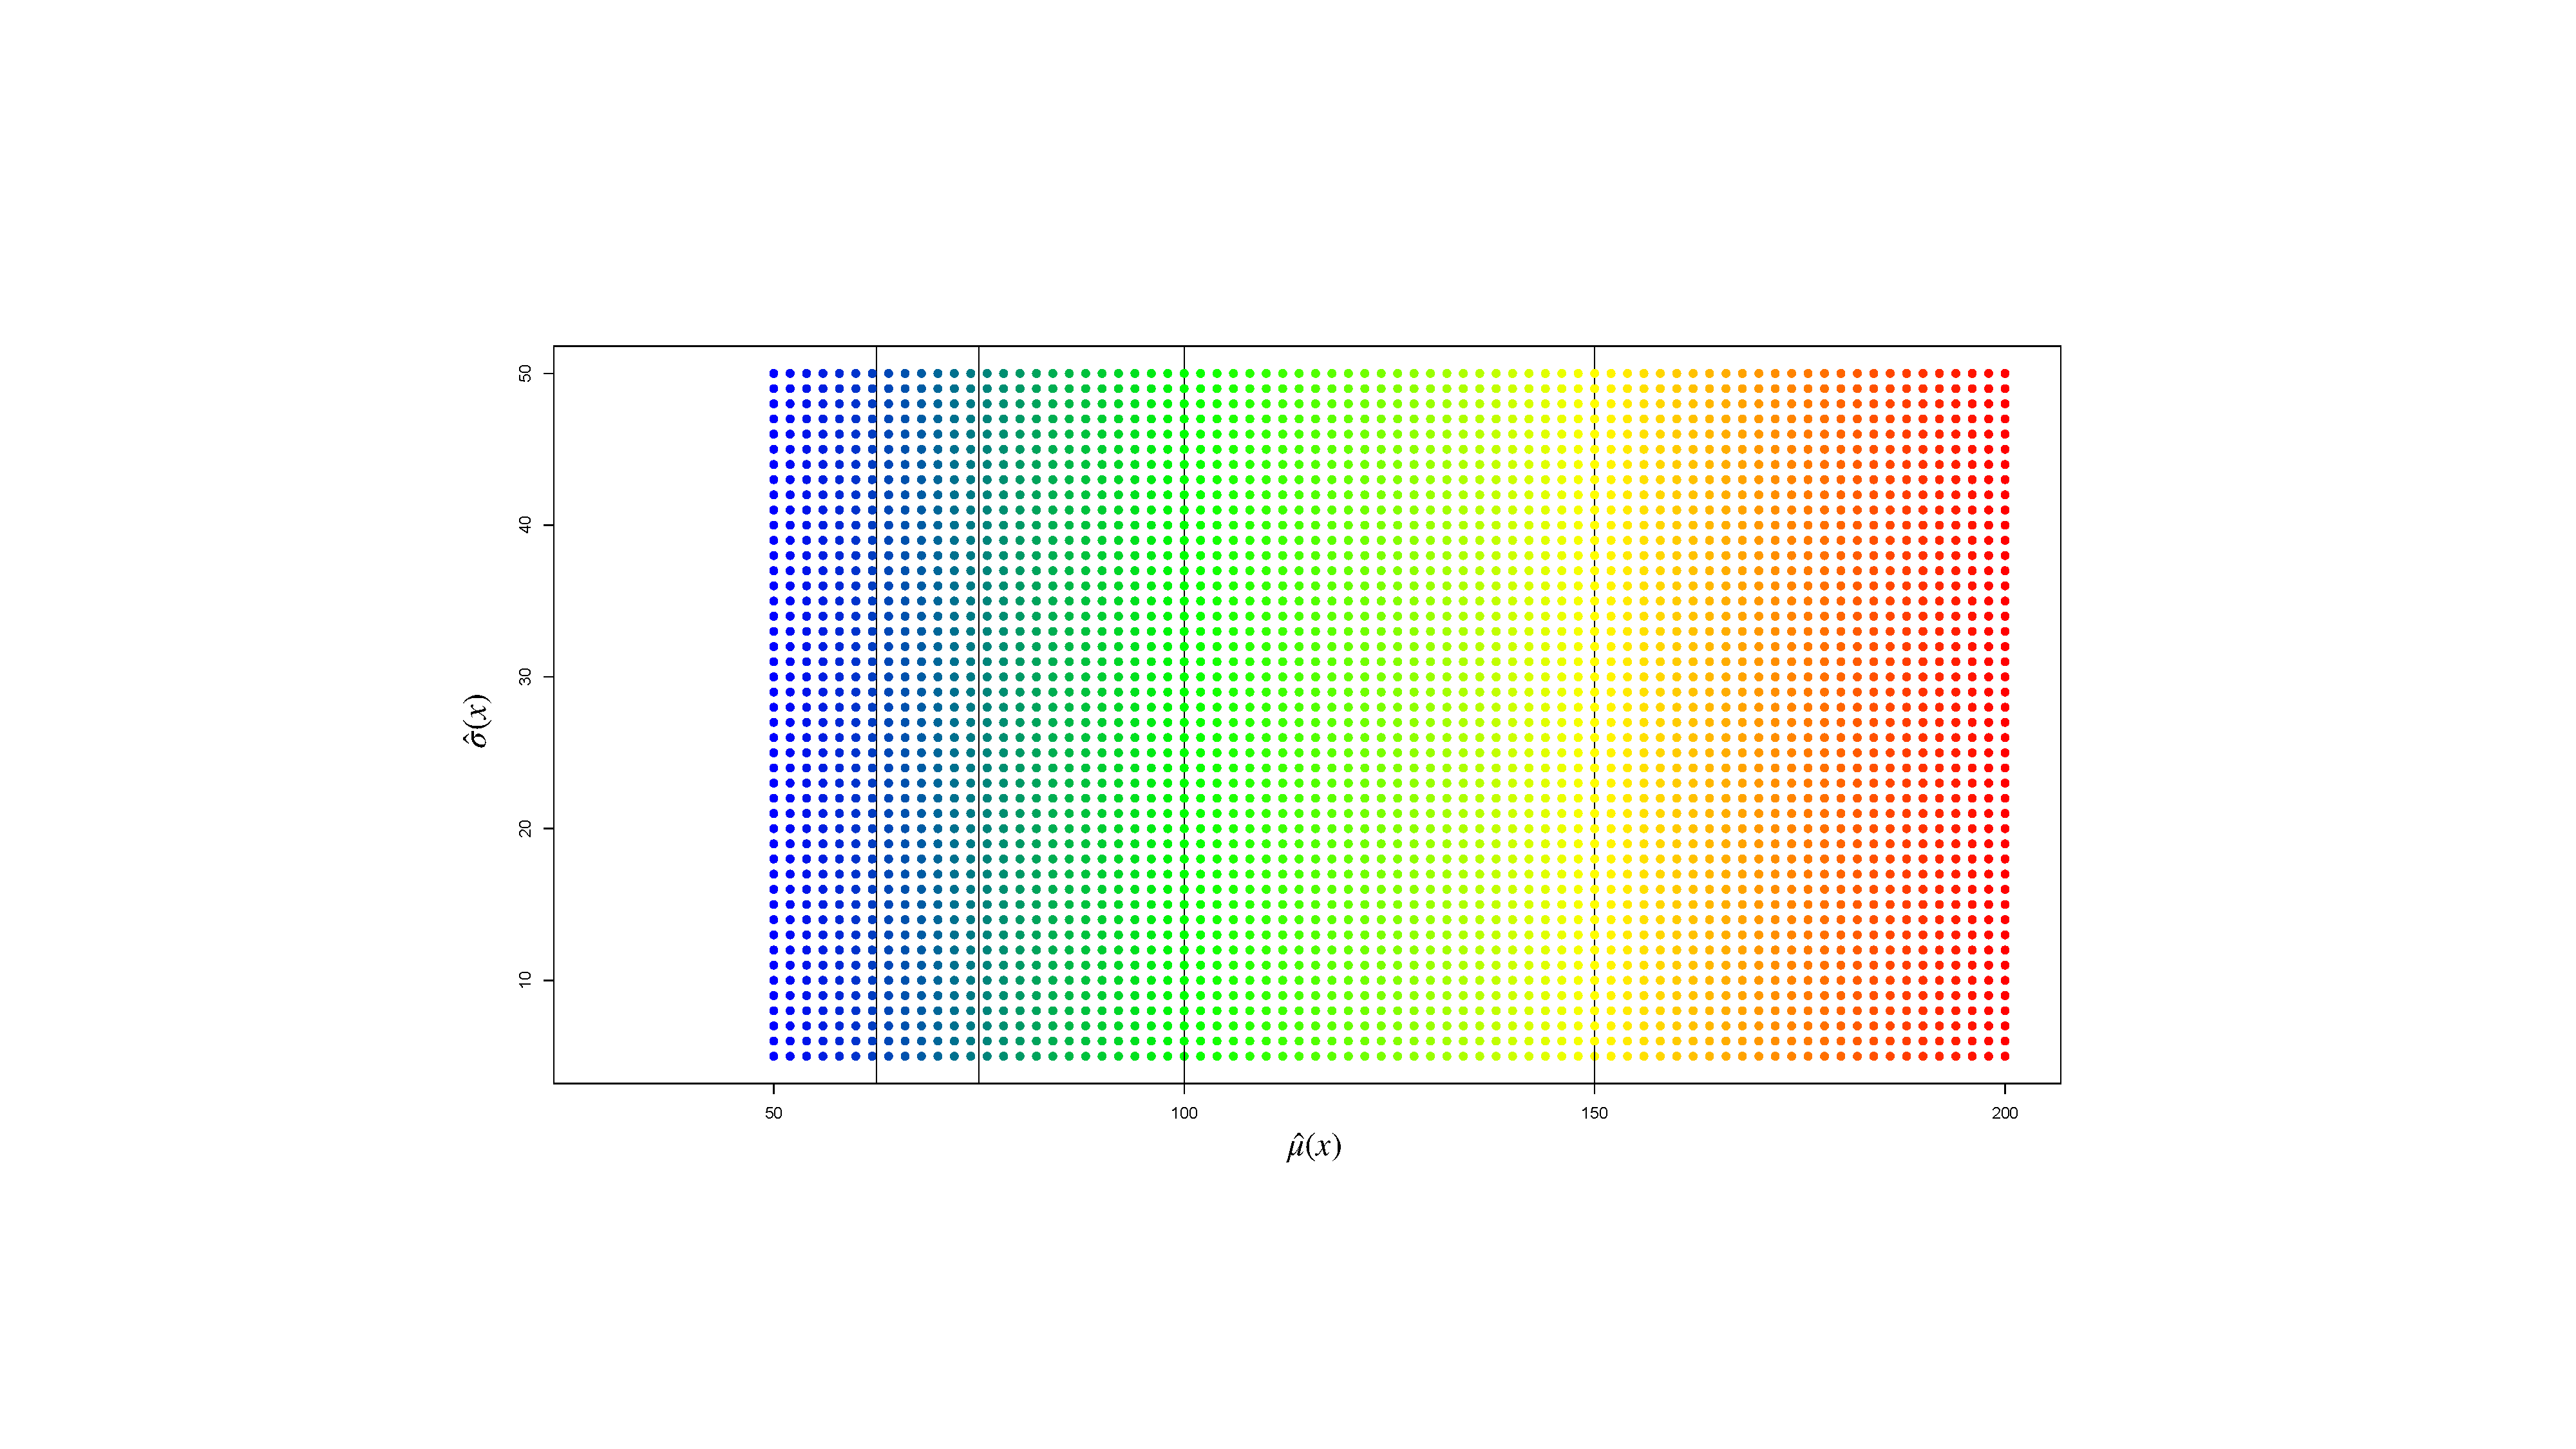
\includegraphics[scale=0.3]{Chapter5/Pictures/EV_mean}
    \caption{Plot showing the characteristics of choosing }
    \label{fig:EV_1.5}
\end{figure}





\begin{figure}[h!]
    \centering
    \subfloat[$\epsilon=0$]{
    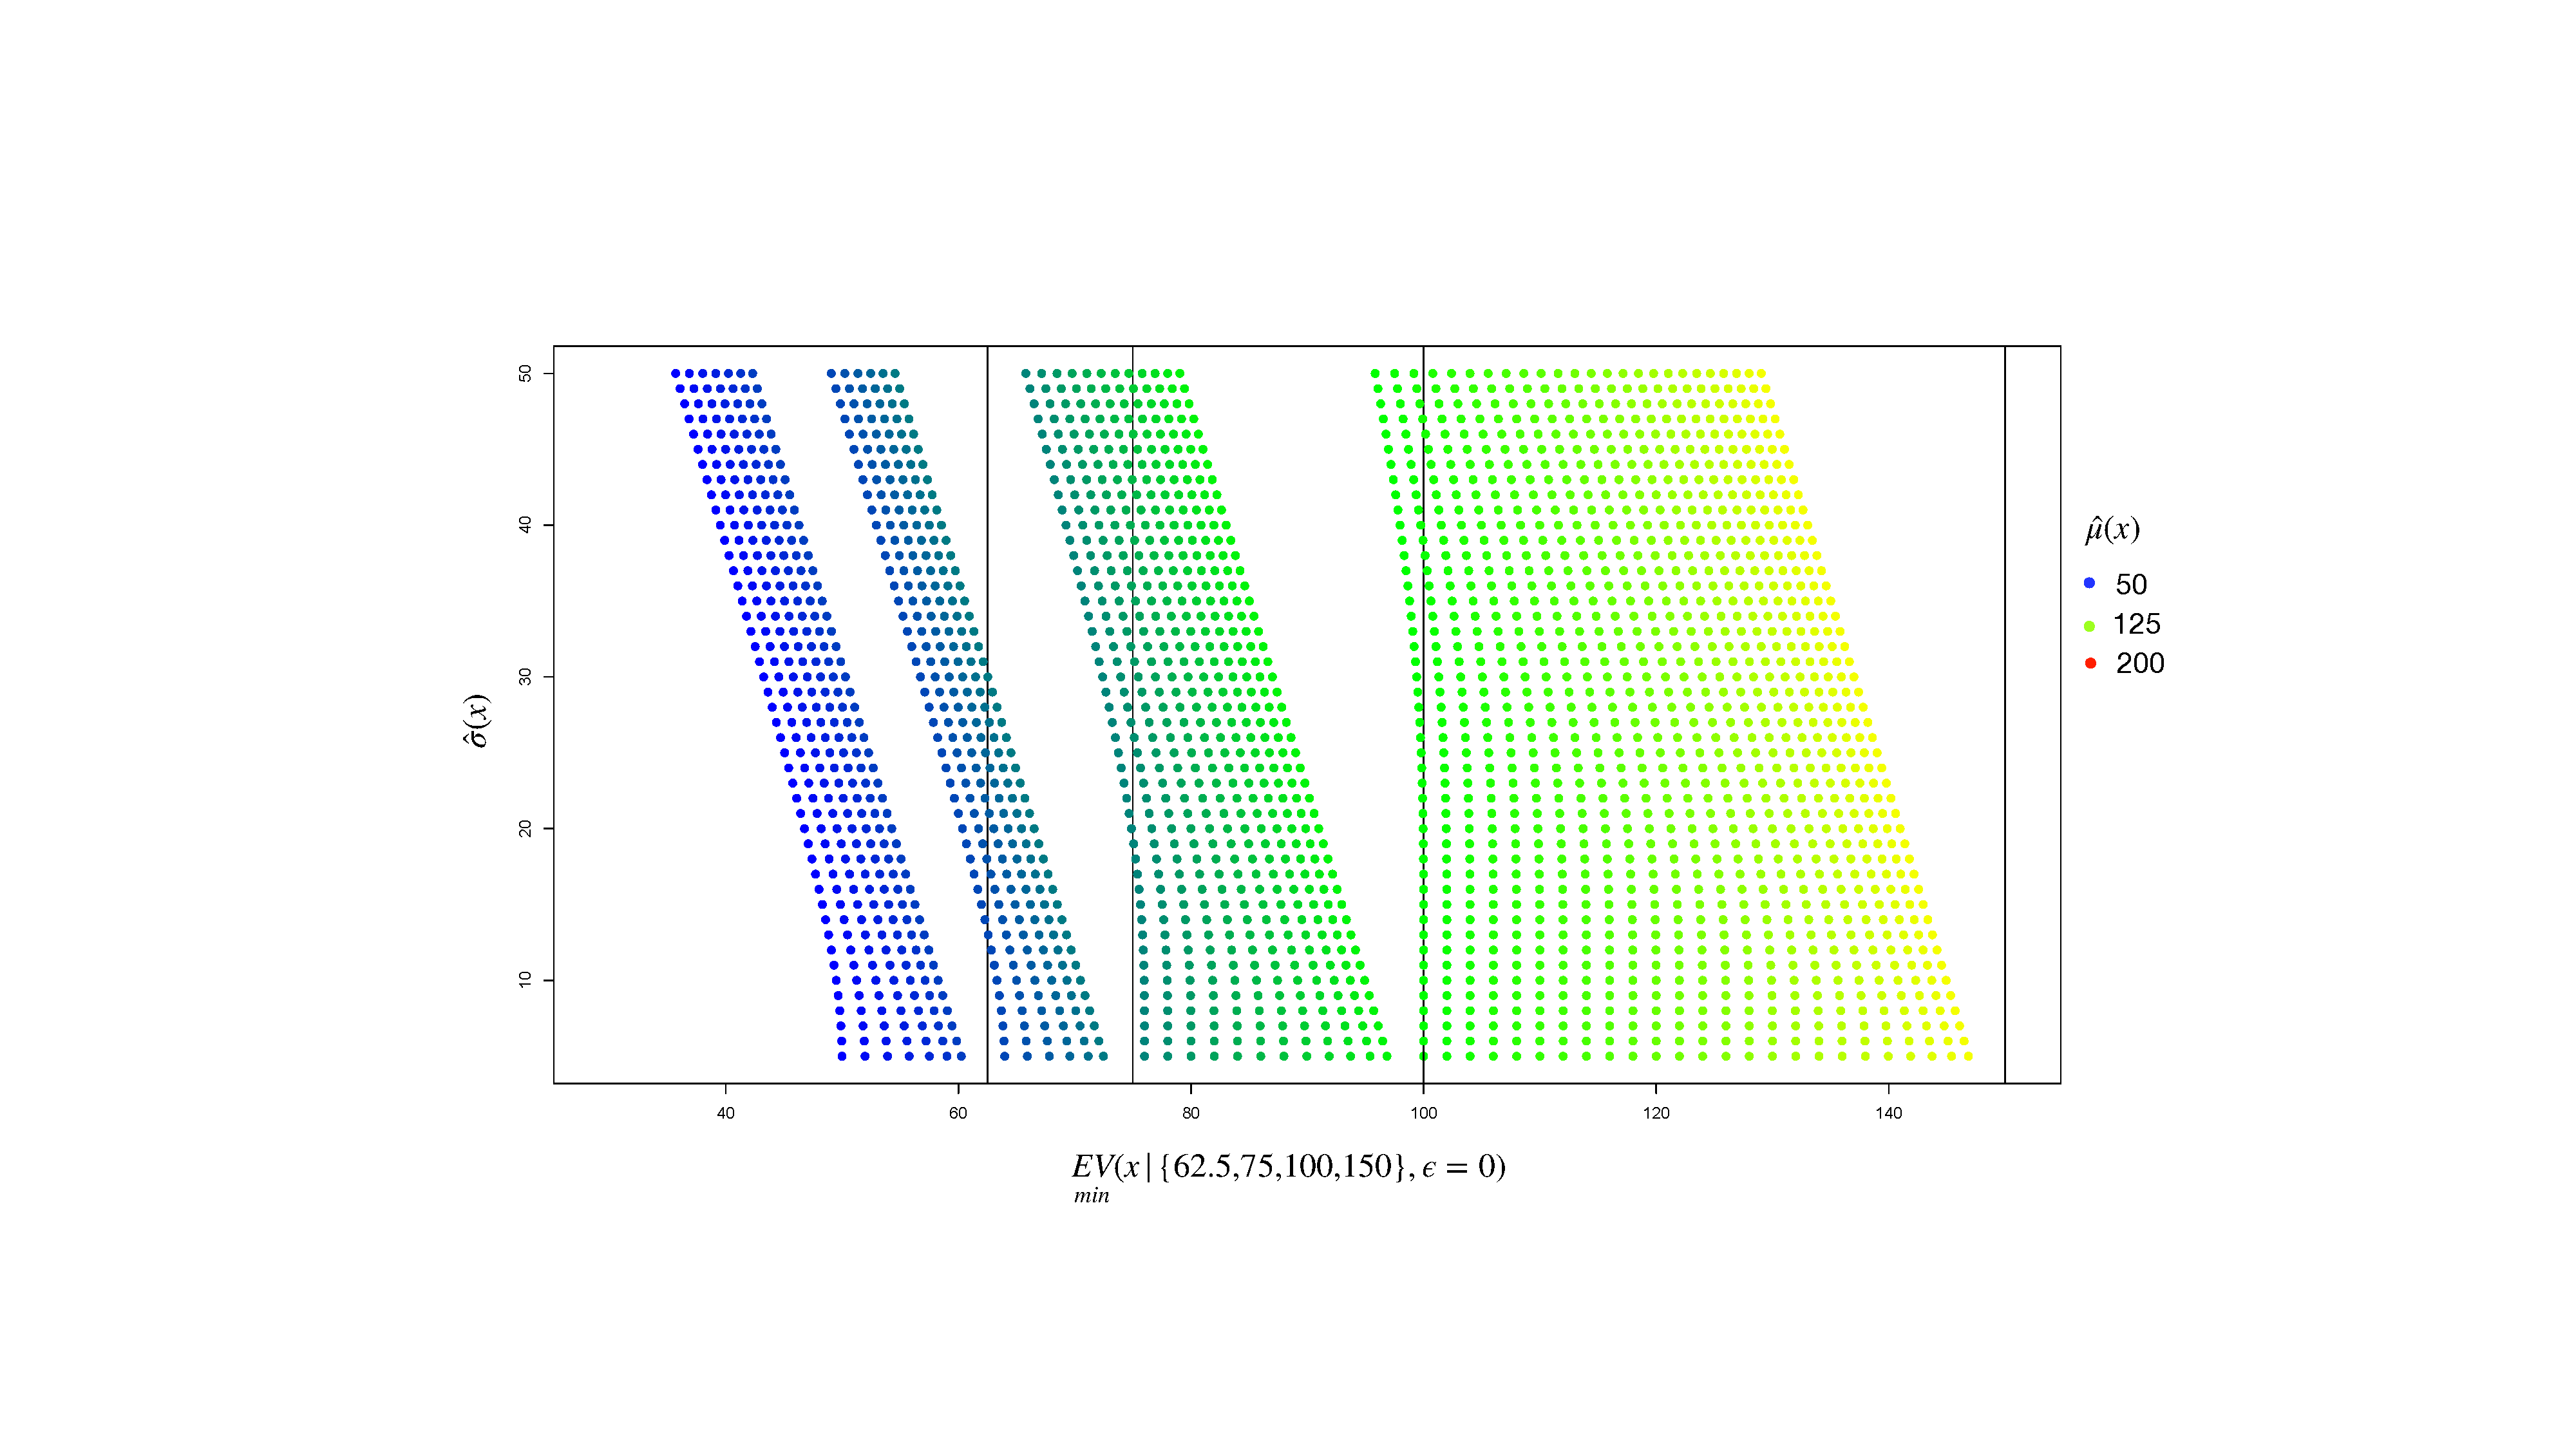
\includegraphics[scale=0.3]{Chapter5/Pictures/EV_0}}\\
    \subfloat[$\epsilon=0.5$]{
    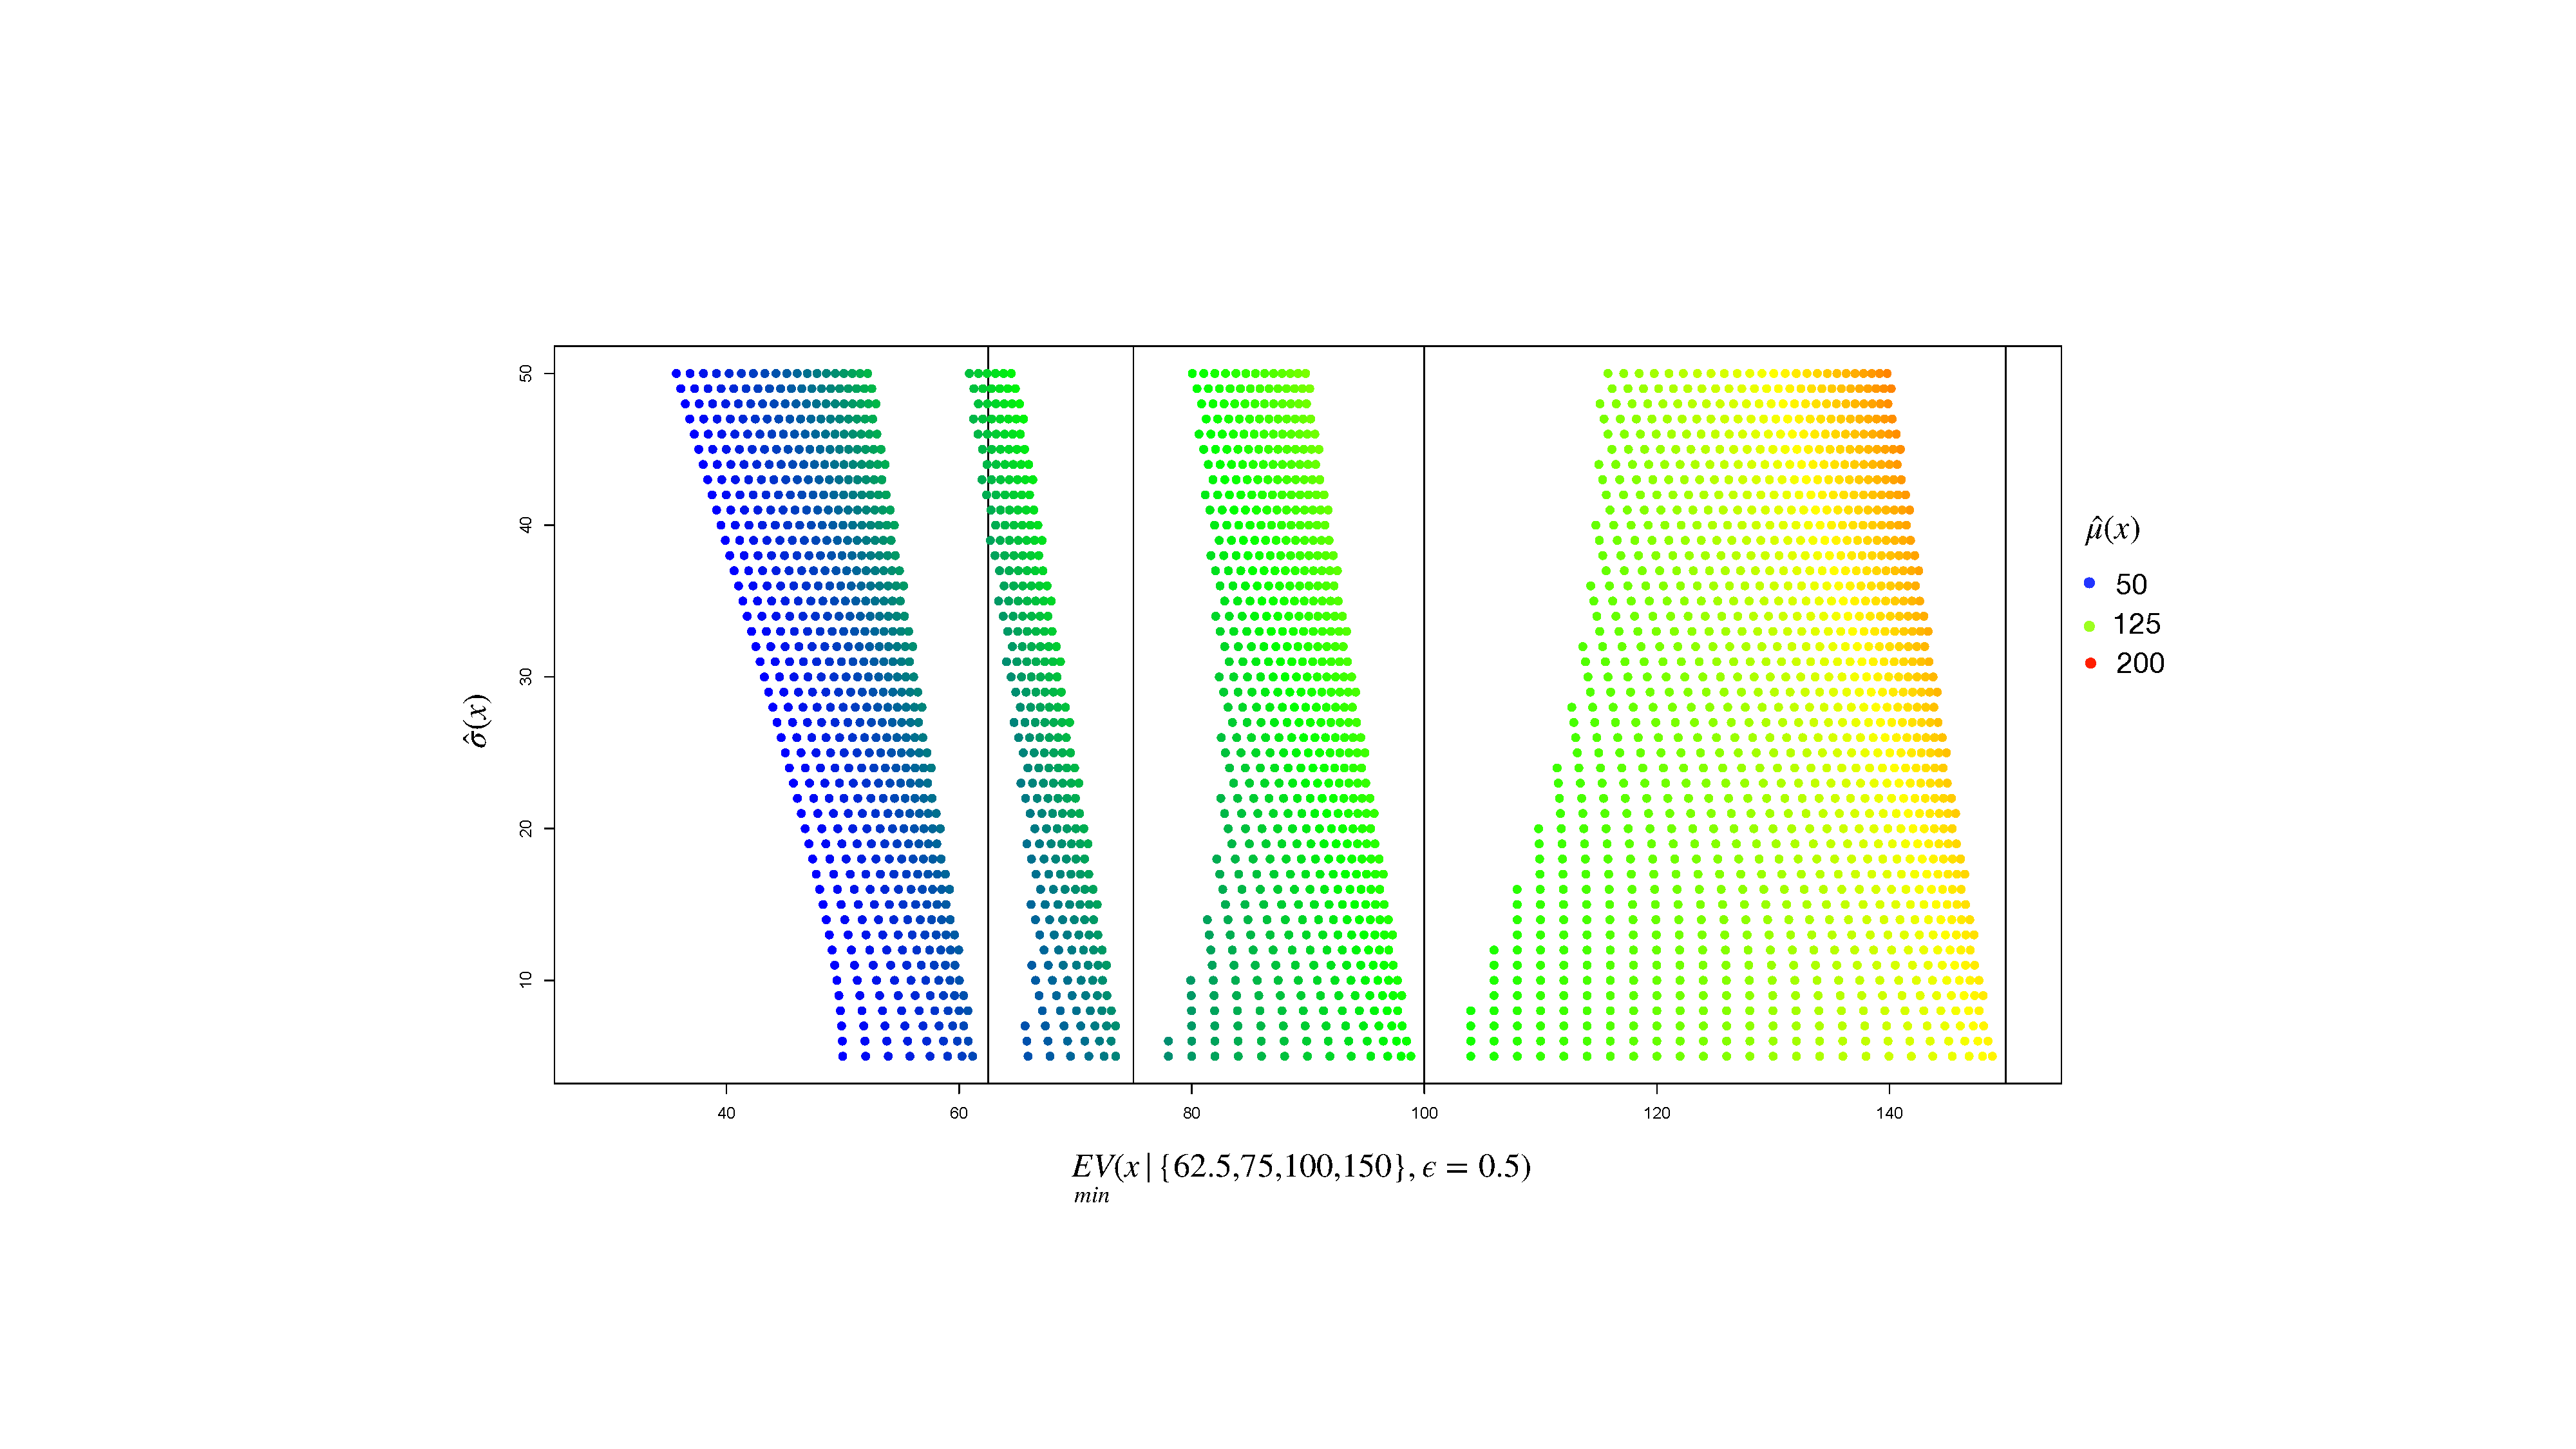
\includegraphics[scale=0.3]{Chapter5/Pictures/EV_05}}
    \end{figure}
\clearpage
    
   \begin{figure}[h!]
    \centering 
    \subfloat[$\epsilon=1$]{
    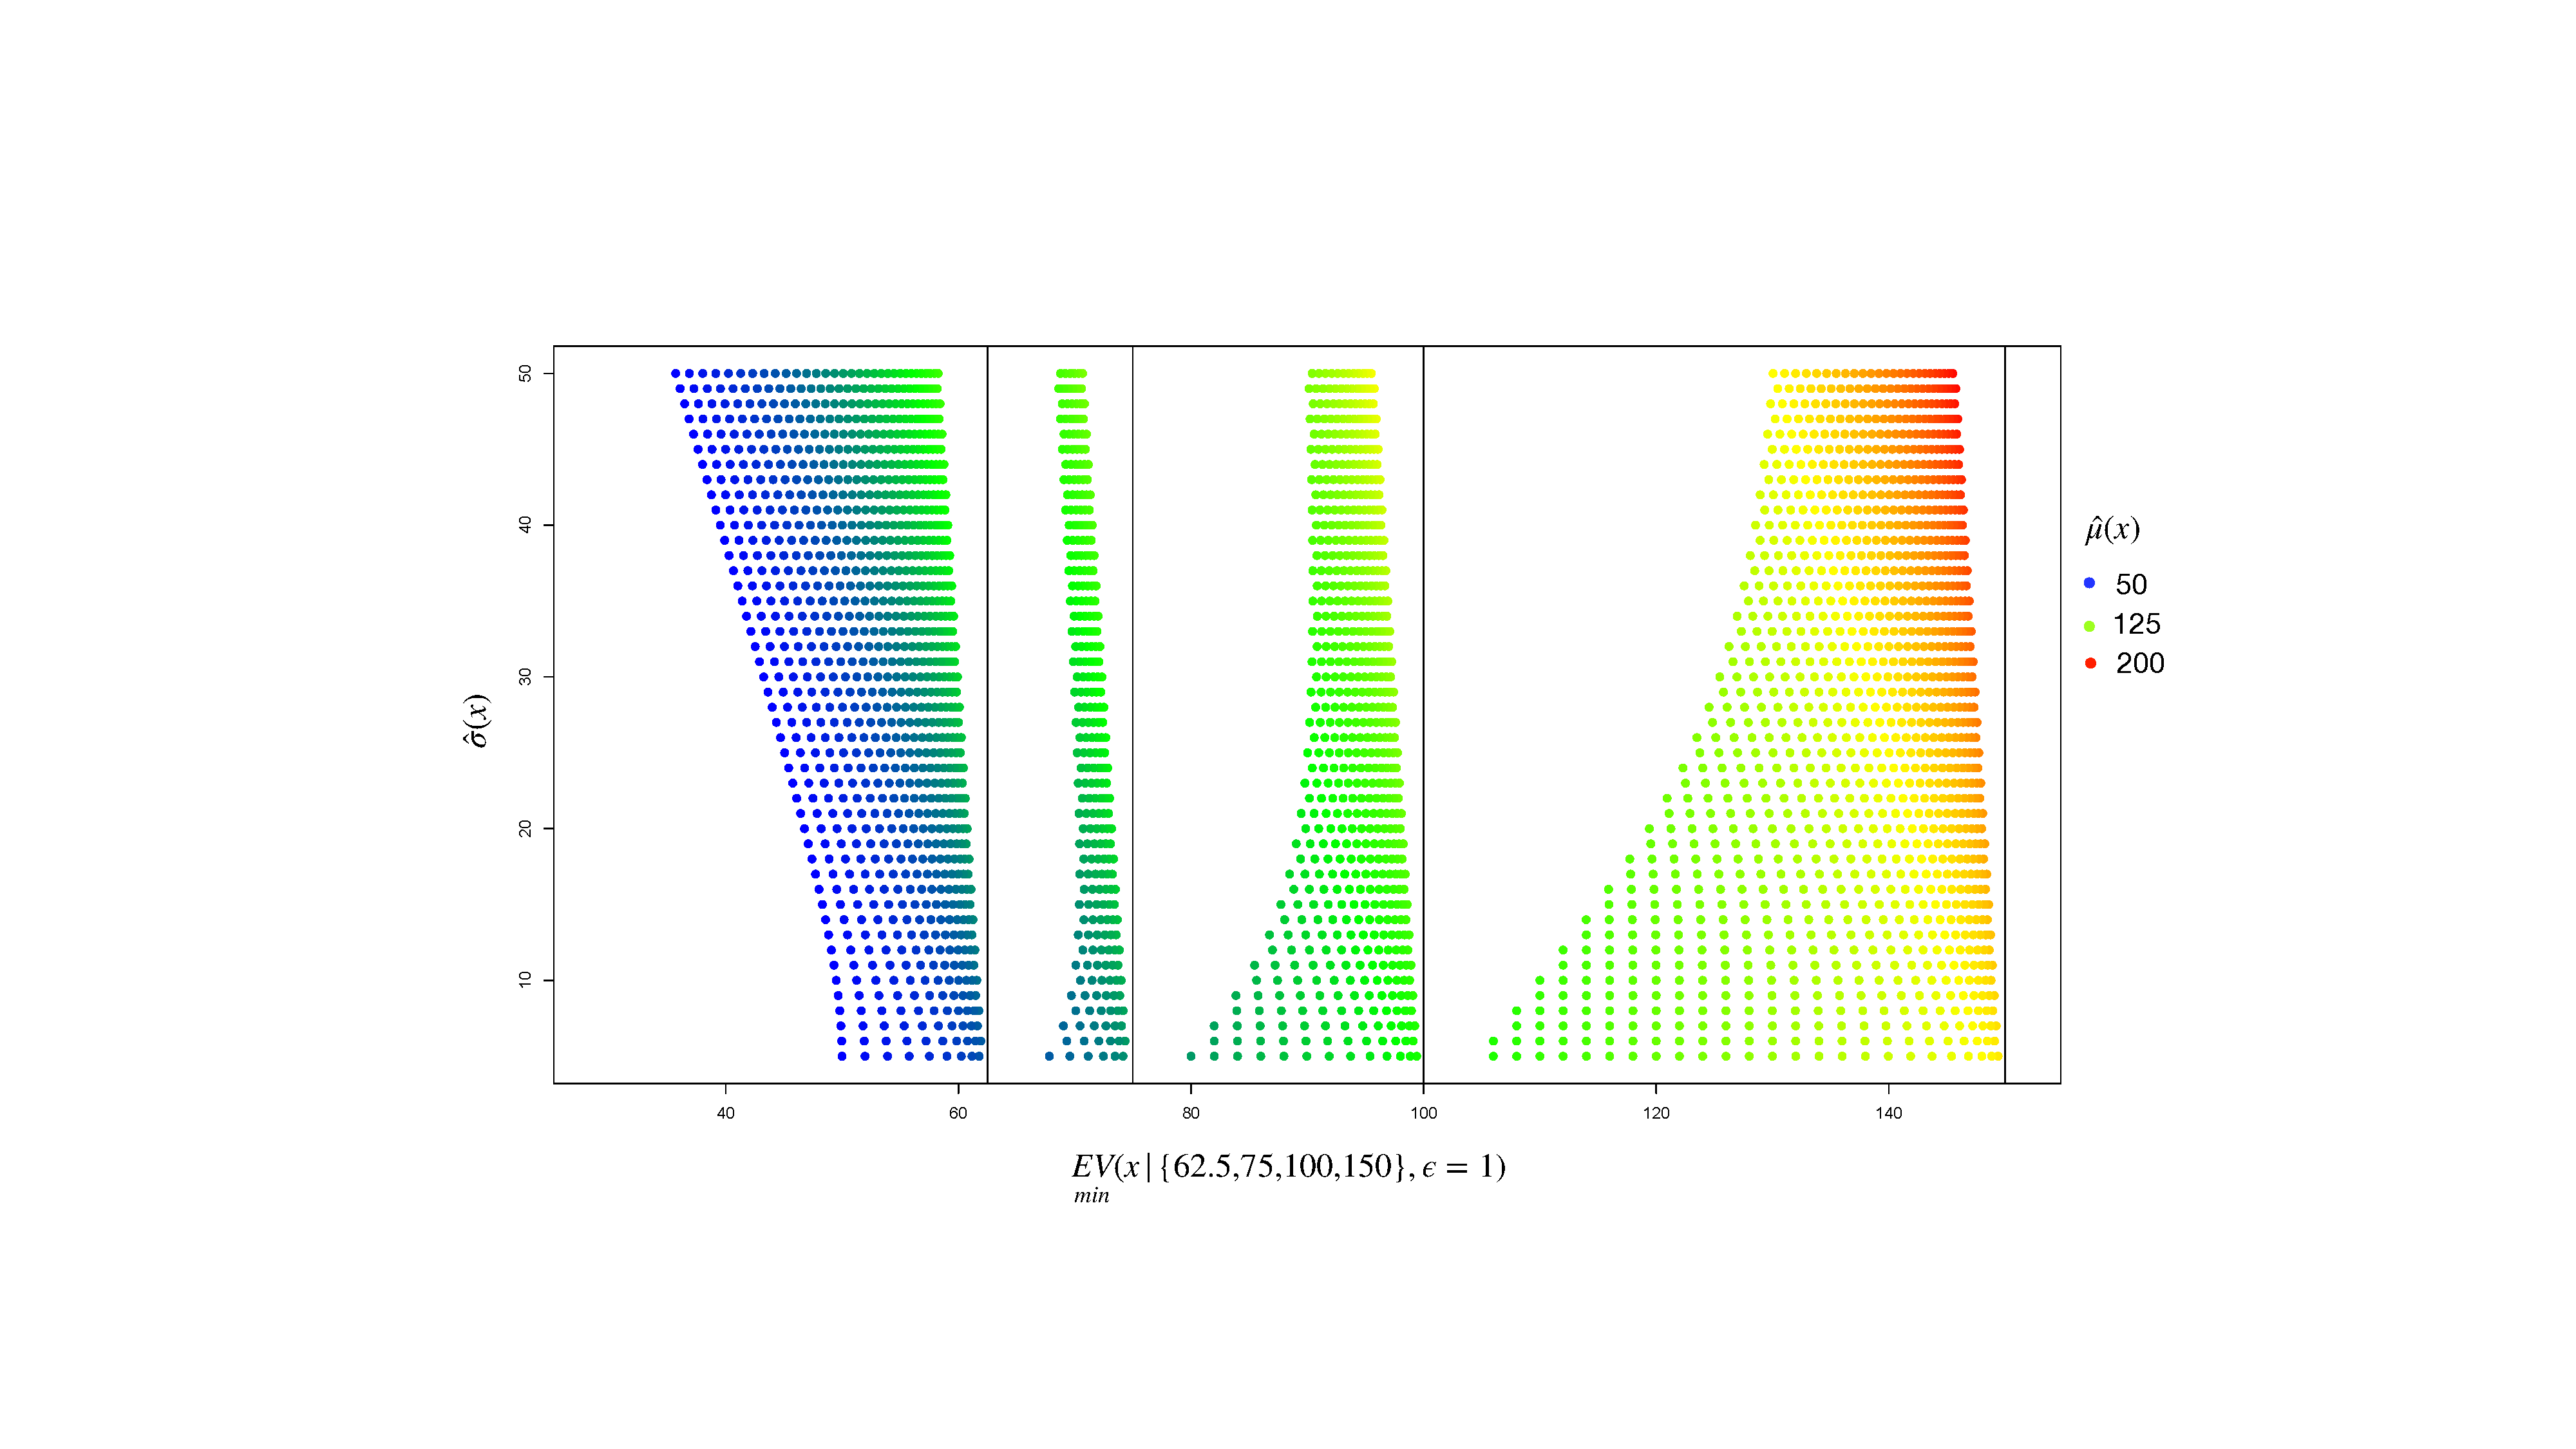
\includegraphics[scale=0.3]{Chapter5/Pictures/EV_1}}\\
    \subfloat[$\epsilon=1.5$]{
    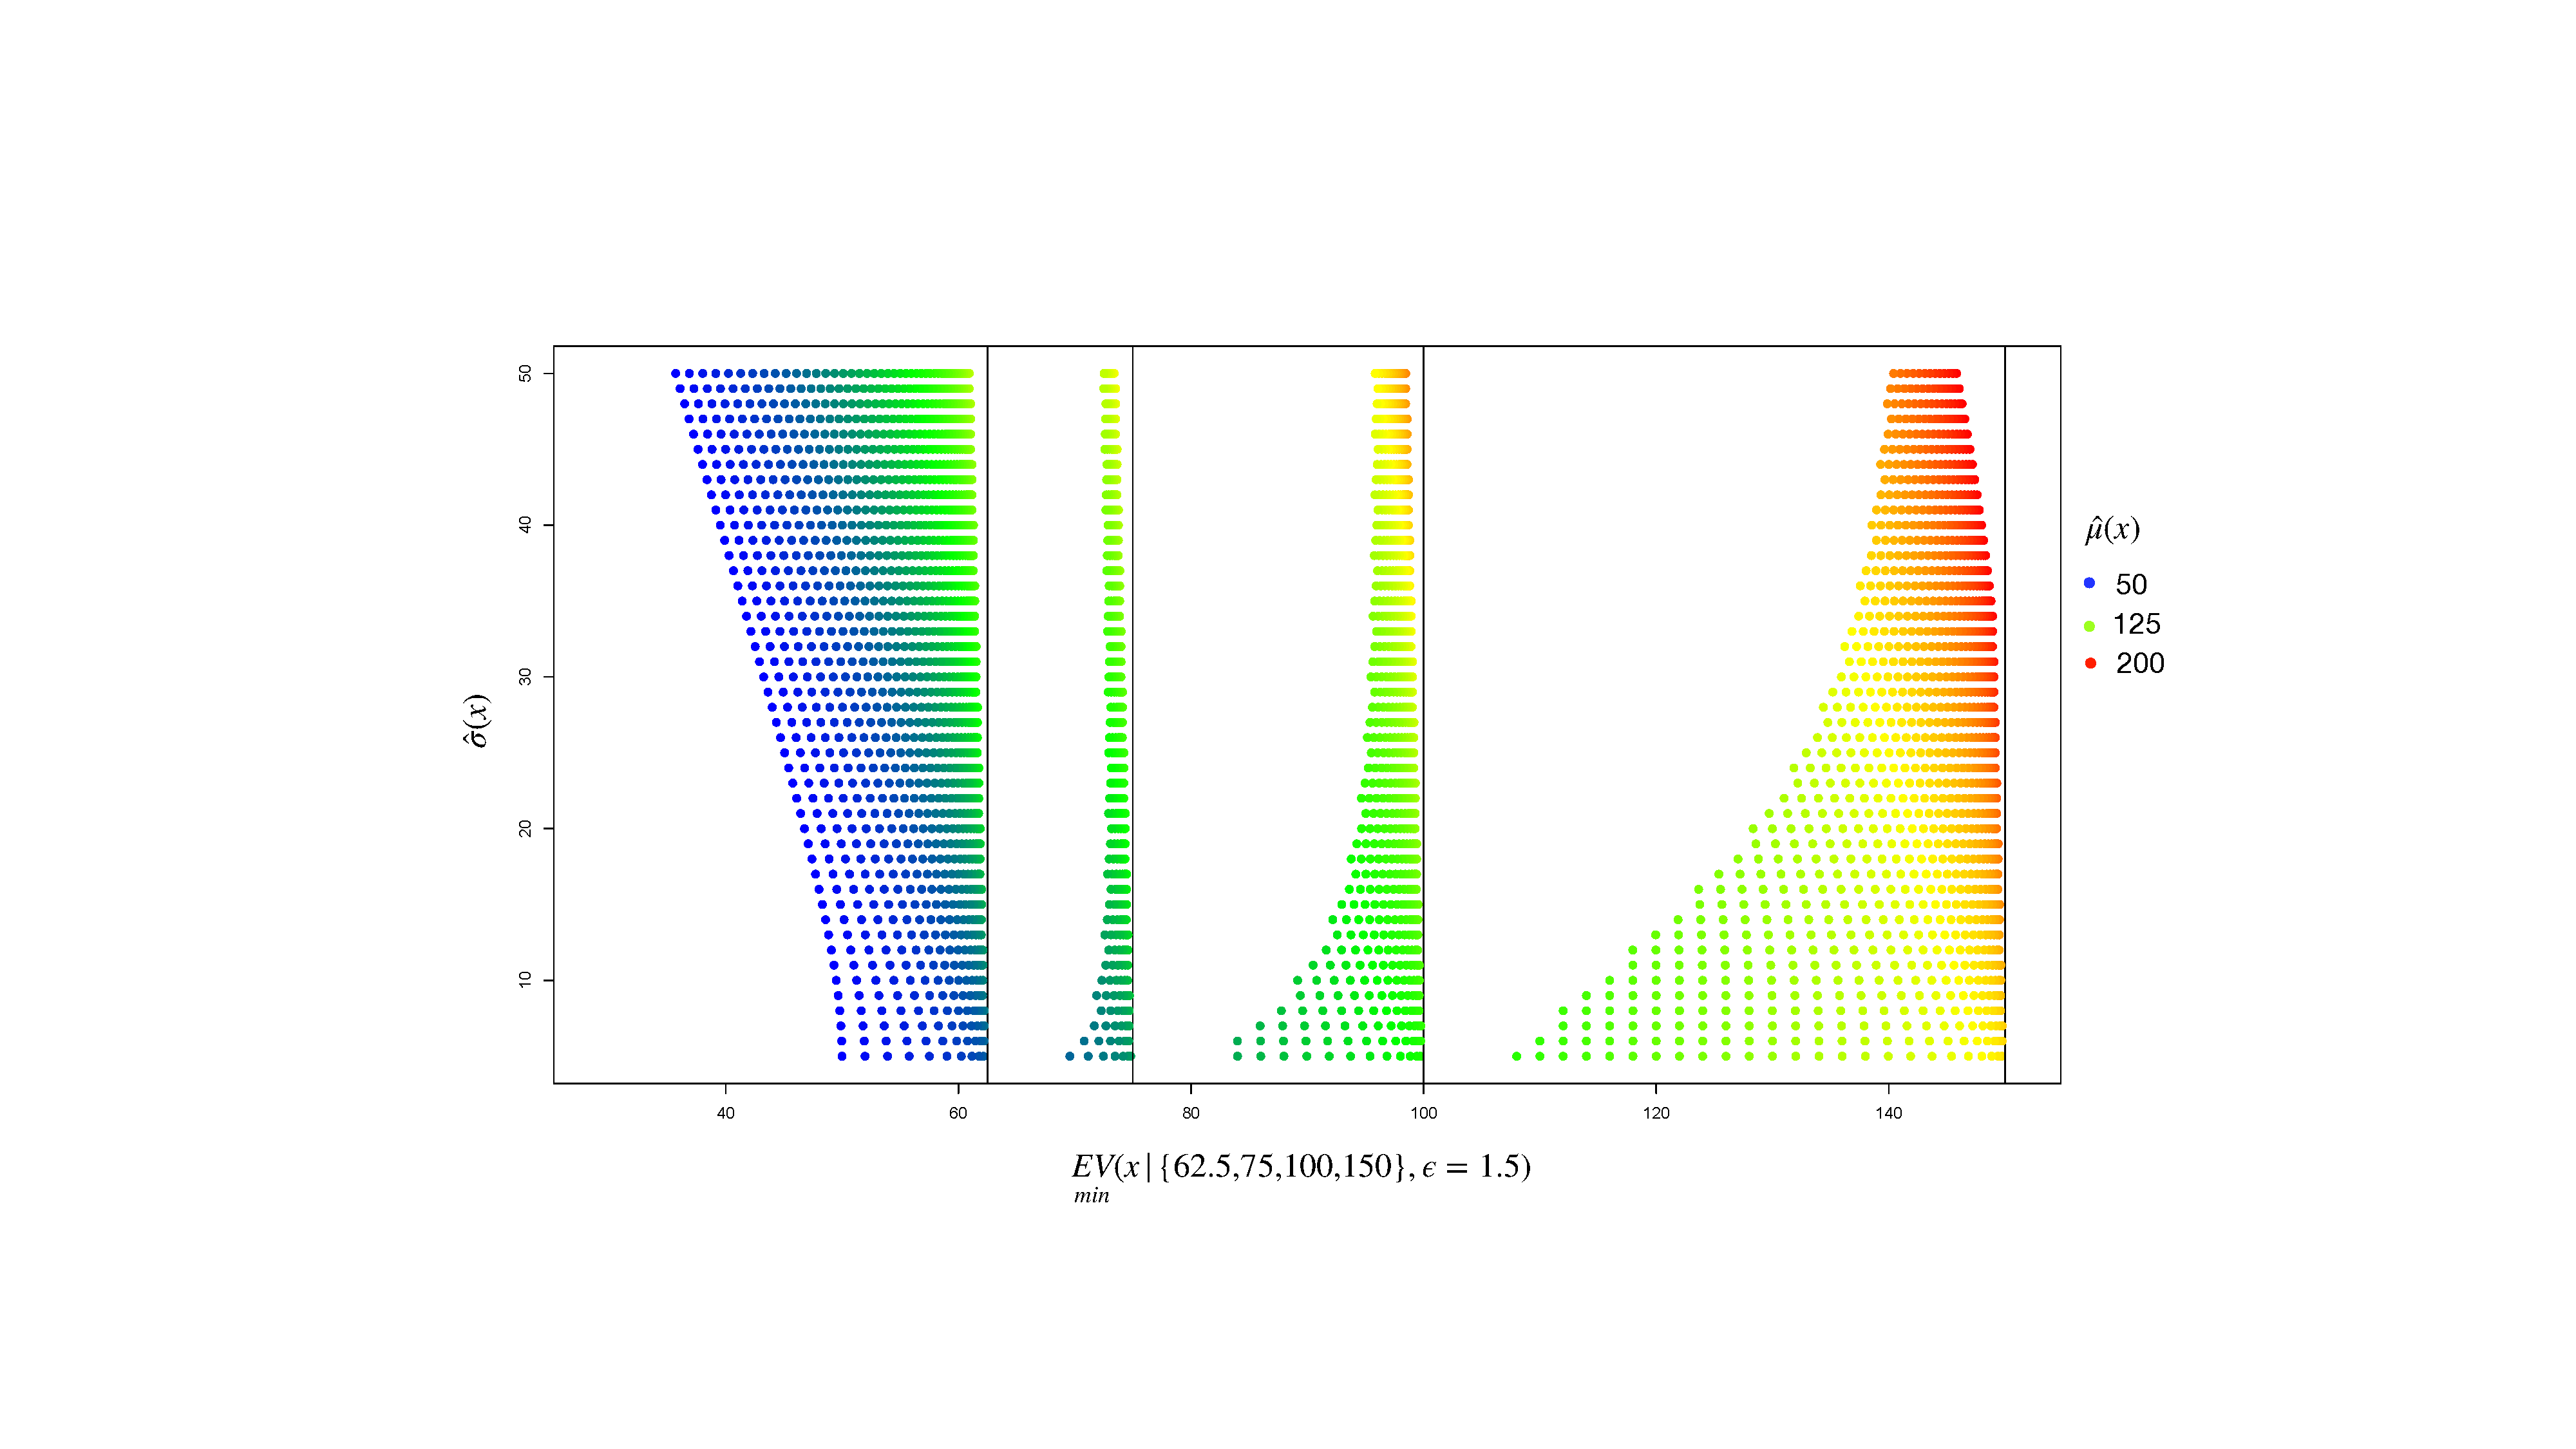
\includegraphics[scale=0.3]{Chapter5/Pictures/EV_15}}
\end{figure}

Some of the special cases where it converges to the cases of Nadir to Utopian value of reference is shown below

\begin{figure}[h!]
    \centering
    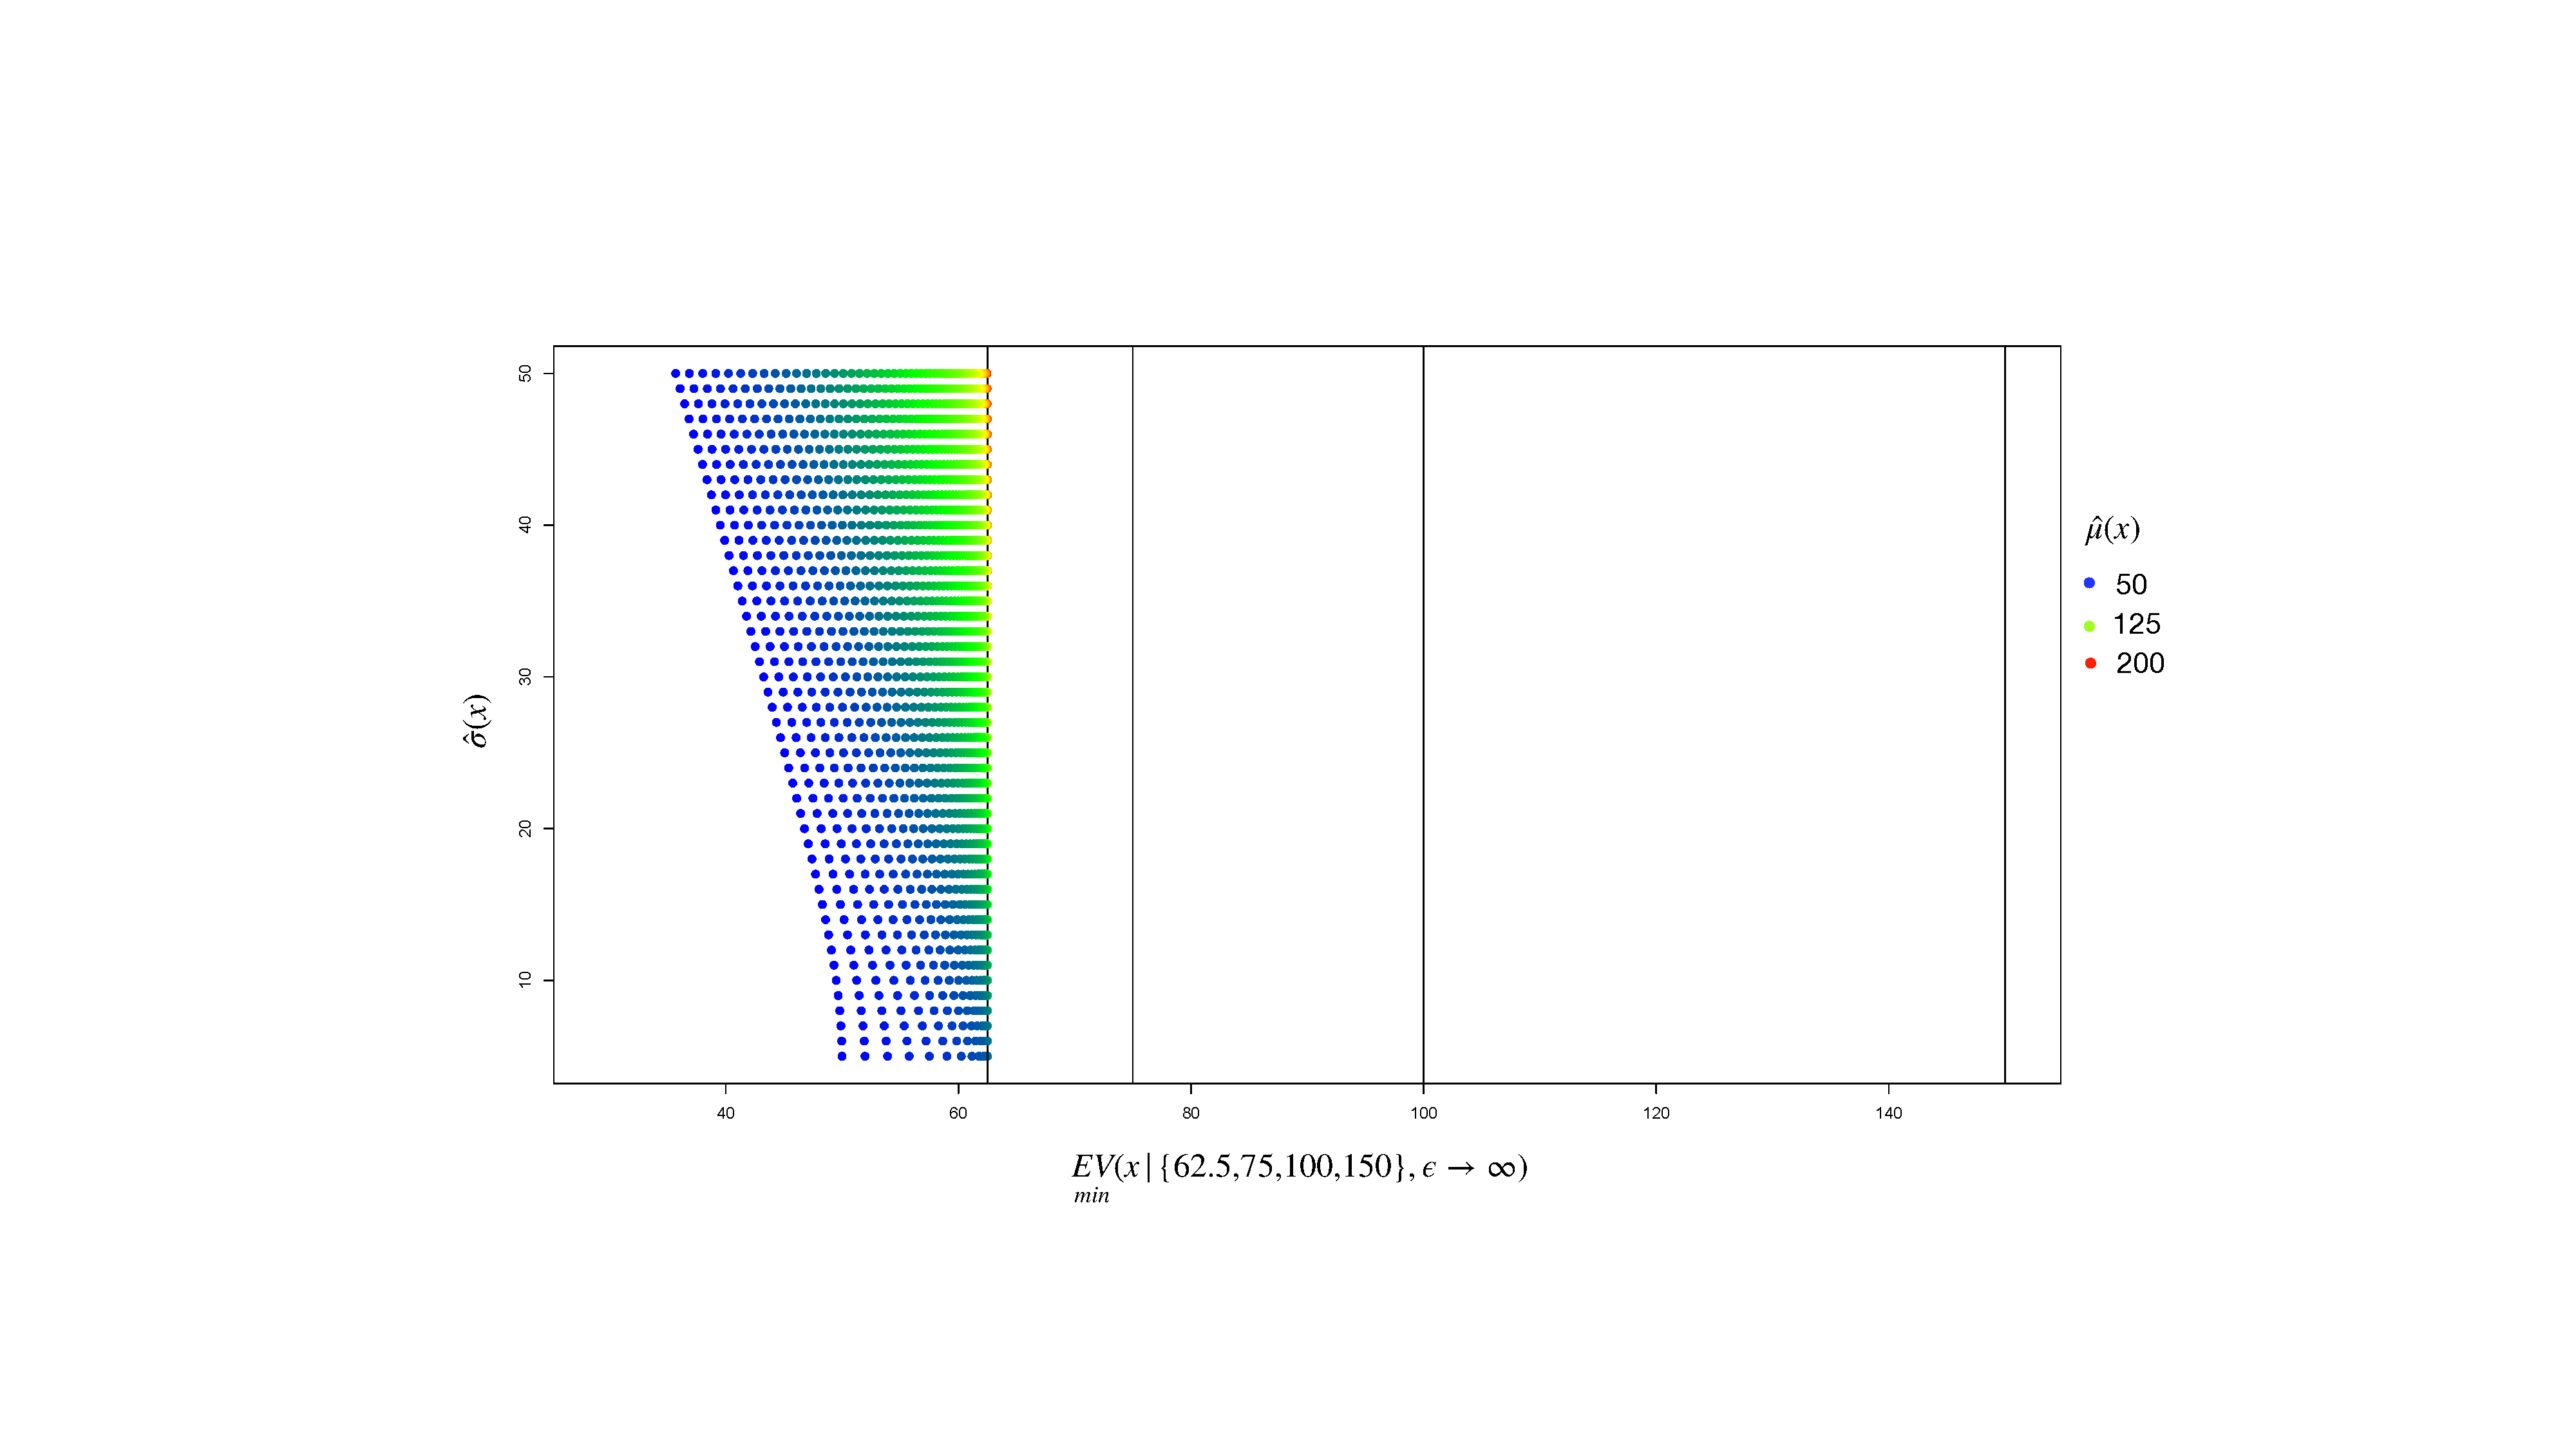
\includegraphics[scale=0.3]{Chapter5/Pictures/EV_inf}
    \caption{ $\epsilon \rightarrow \infty$}
    \label{fig:EV_1.5}
\end{figure}

\begin{figure}[h!]
    \centering
    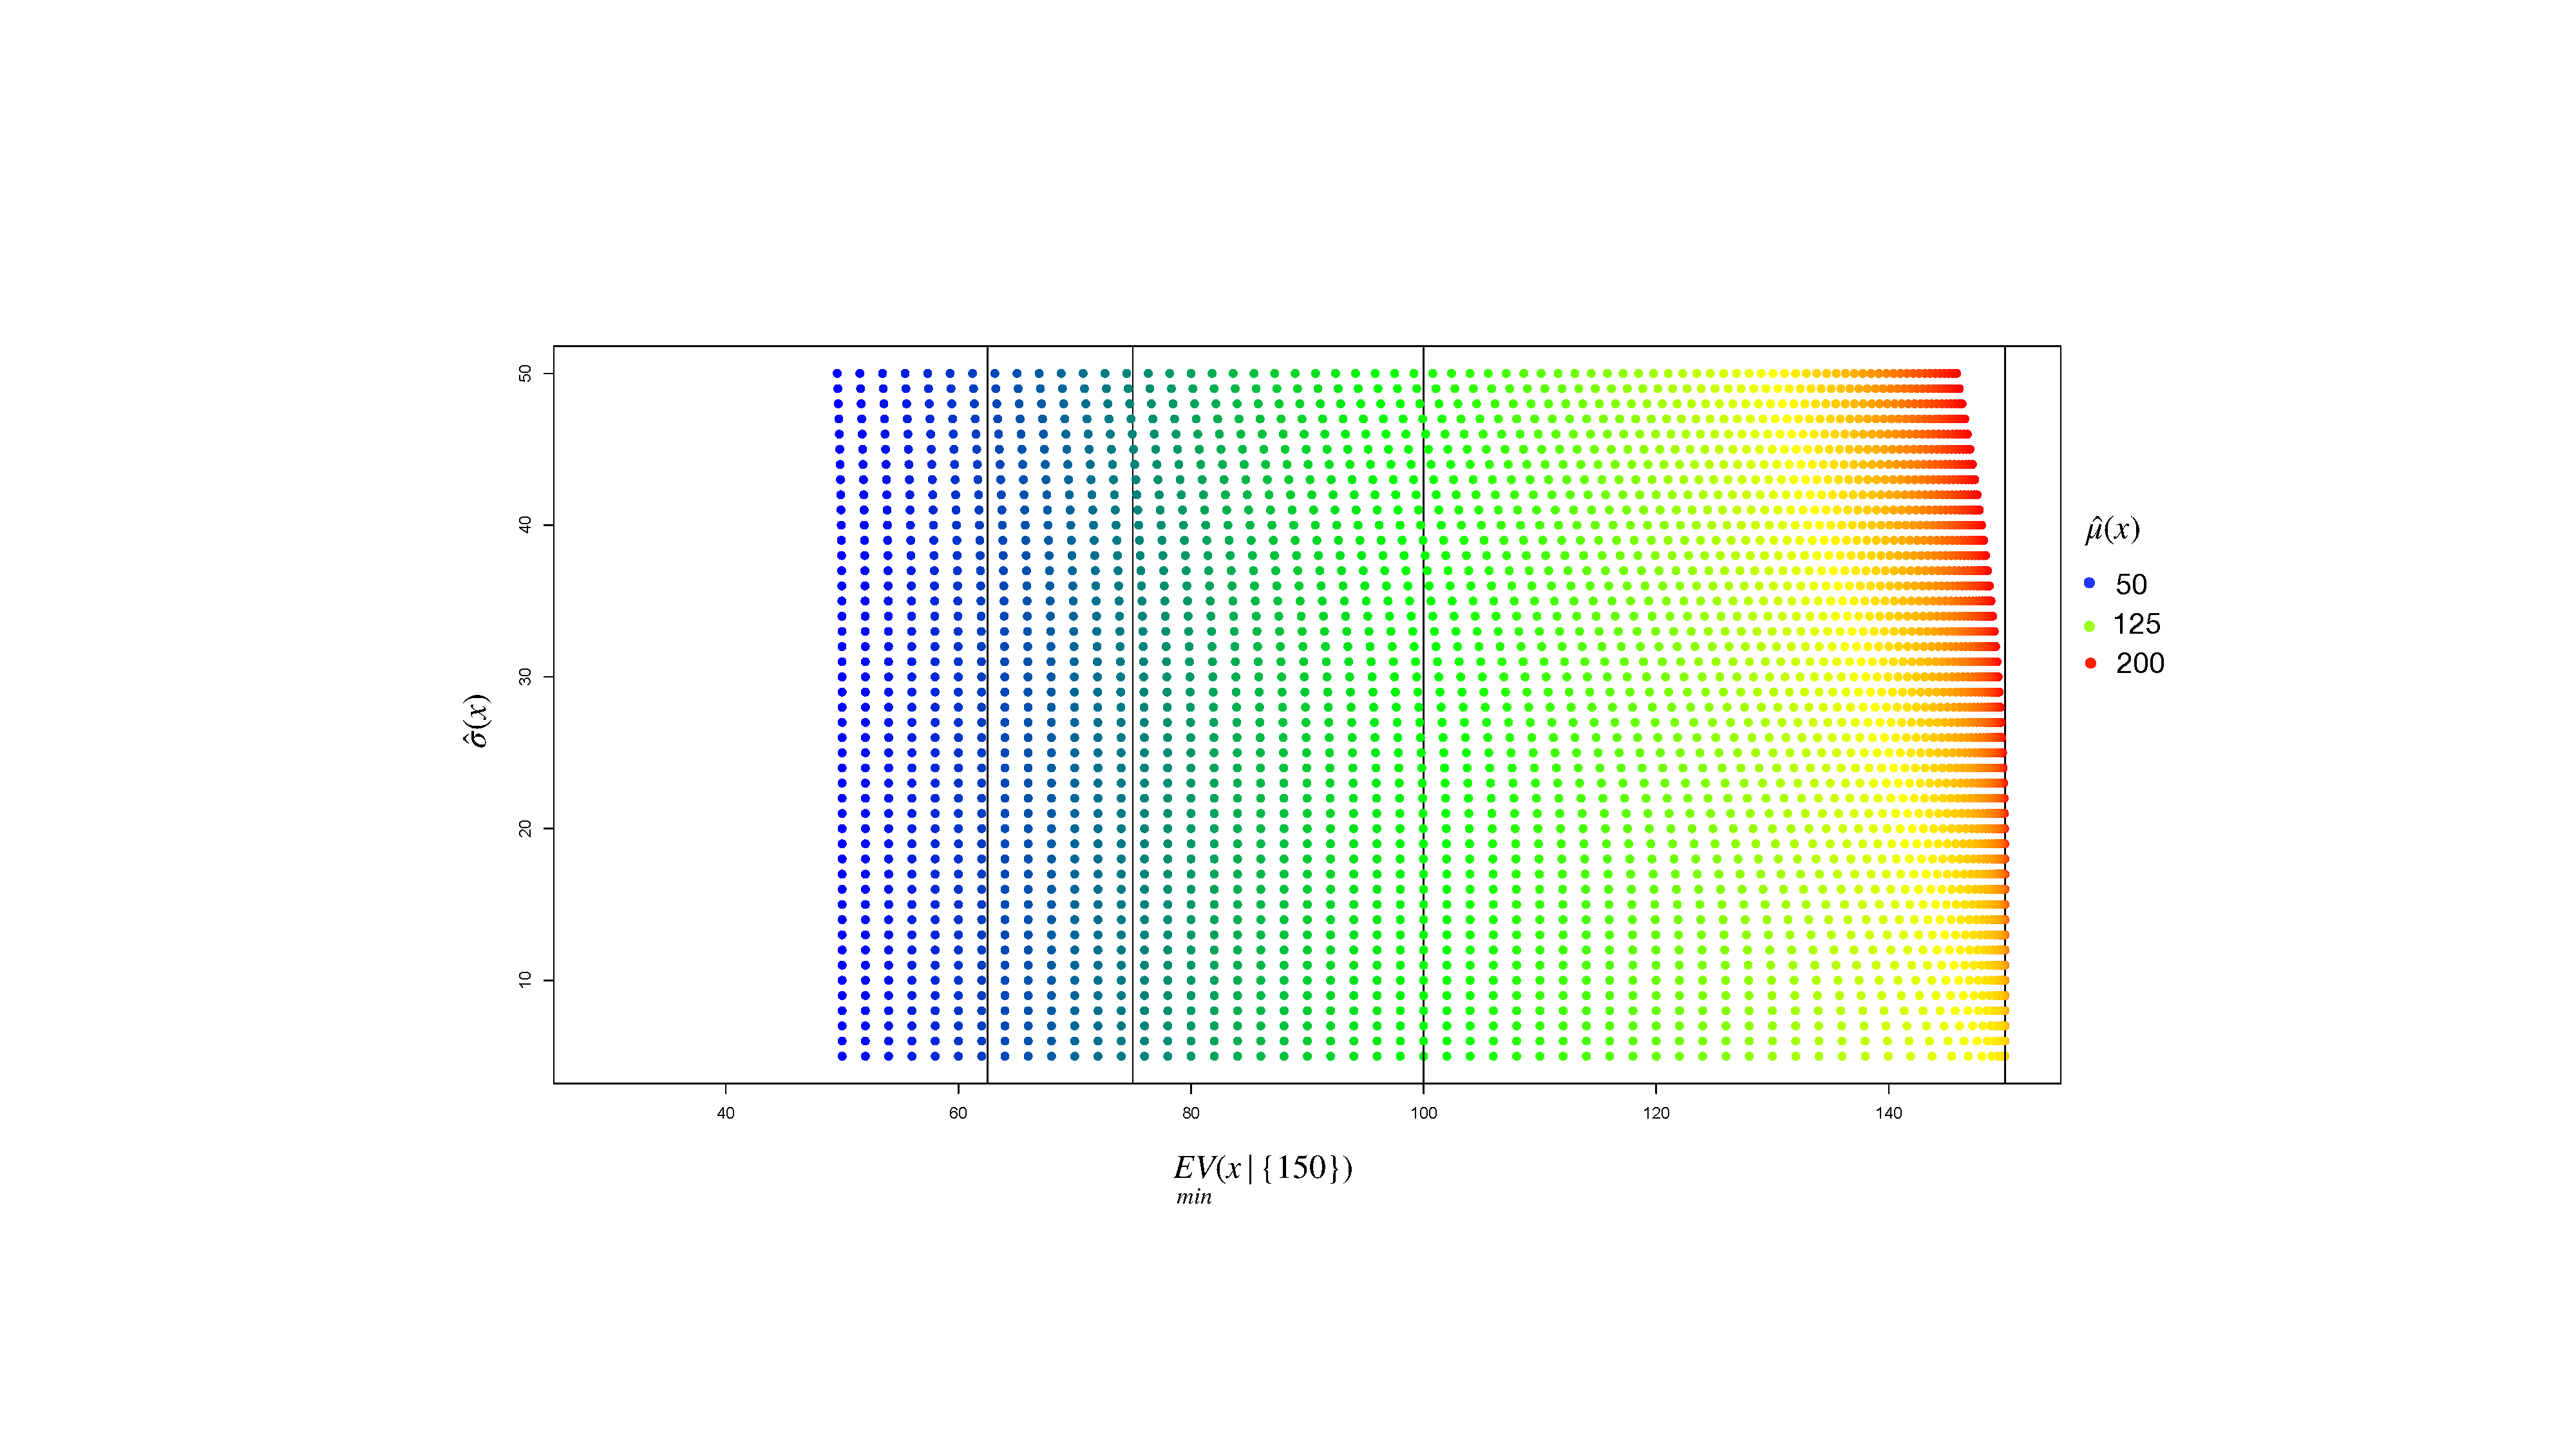
\includegraphics[scale=0.3]{Chapter5/Pictures/EV_nad}
    \caption{EV with Nadir value as reference}
    \label{fig:EV_1.5}
\end{figure}











\input{Chapter6/IGA_based.tex}
%\input{Conclusion/Conclusion.tex}


%\subsection{IGA formulation}
%\chapter{IGA formulation}
\cite{ha2015}
We start with the definition of B-spline functions with extension to B-spline curves, from which NURBS curves are introduced with the definition of a weighing parameter and a non-uniform knot vector. This is followed by description of higher dimensional geometries through extension by tensor product definition.\\
 
 The B-spline basis functions can be defined by Cox de Boor's formula as follows,
 
\begin{equation}
{N_{i,0}\left( \xi  \right)} = \left\{ {\begin{array}{cl}
   1 & {\;{\xi _i} \le \xi  < {\xi _{i + 1}}}  \\
   0 & {\;otherwise}
\end{array}} \right.
\end{equation}

\begin{equation}
{N_{i,p}\left( \xi  \right)} = \frac{{\xi  - \xi_{i} }}{{{\xi _{i + p}} - {\xi _i}}}{N_{i,p - 1}\left( \xi  \right)} + \frac{{{\xi _{i + p + 1}} - \xi }}{{{\xi _{i + p + 1}} - {\xi _{i + 1}}}}{N_{i + 1,p - 1}\left( \xi  \right)}
\end{equation}

where $p$ is defined recursively for $p>0$ to obtain a curve of degree $p$, which starts with a piecewise constant at $p=0$. Naturally, a uniform knot vector can be defined as  $\bm \xi  = \left\{ {{\xi _1},{\xi _2}, \cdots ,{\xi _{n + p + 1}}} \right\}$, where any $\xi_i - \xi_{i+1}$ is uniformly spaced.  
For a uniform knot vector, the bases span with continuity $C^{p-1}$ between the knots, where it satisfies partition of unity $\sum_{i=1}^{n} {N_{i,p}\left( \xi  \right)} = 1$ for $[\xi _p,\xi _{n+1}]$, with $n$ being the number of control points. Further, the span of any ${N_{i,p}\left( \xi  \right)}$ is defined in $[\xi_i,\xi_{i+p+1}]$, and ${N_{i,p}\left( \xi  \right)} \geq 0$, $\forall \xi$.\\

The knot vector need not be equidistant and the multiplicity  of a knot $\xi _i$ by $\mathcal{M}$ in the knot vector decreases the continuity by $C^{p-\mathcal{M}}$ across the knot $\xi _i$,  which defines a non-uniform knot vector. 
The multiplicity $\mathcal{M}=p$ for the first knot and the last knot defines a open knot vector, where the basis functions model interpolation between the first and the last knots. 
The basis functions defined with an open knot vector satisfies partition of unity $\forall \xi$. 
Through B-spline basis functions and a knot vector $\bm \xi  = \left\{ {{\xi _1}, \cdots ,{\xi _{n + p + 1}}} \right\}$, a B-spline curve can be defined with coefficients of the basis functions as follows 

\begin{equation}
\bm X_c(\xi) =  \sum_{i=1}^n N_{i,p}(\xi)  \bm {{P}}_i
\end{equation}

where with a open knot vector for a curve, the ends of the curve are $C^0$. The coefficients $\bm{{P}}_i \in \mathbb{R}^{d}$ are the control points, with $d$ being the dimension of the space. The definition of a weighing parameter $w_i >0$ associated with a re spective basis function $N_i$, normalized defines rational B-splines where it respects the partition of unity, given as follows
\begin{equation}
\bm X_c(\xi) =  \sum_{i=1}^n\underbrace{\frac{w_iN_{i,p}(\xi)}{\sum_{i=0}^n{w_iN_{i,p}(\xi)}}}_{R_{i,p}}\bm {{P}}_i \label{NURBS_c}
\end{equation}

The parameter $w_i$ provides a new dimension for controlling the geometry through projective transformation, while the affine transformation is achieved by $\bm{{P}}_i$ . Hence, the combination of non-uniform knot vectors and rational basis functions define NURBS. Further, if all weights are the same, NURBS is simply a B-spline with non-uniform knot vector.\\

%Add figure for projective trans IGA book

The higher dimensional NURBS are a natural extension of its $1$-dimensional precursor through tensor product definition where the order of the tensor is the same as the dimension of the geometry. For a $2$-dimensional geometry, the tensor product NURBS surface is defined as follows

\begin{equation}
\bm X_s(\xi,\eta) =   \sum_{i=1}^n\sum_{j=1}^m  R_{i,p}(\xi)R_{j,q}(\eta)\bm{{P}}_{i,j} \label{NURBS_s}
\end{equation}

which is supported by knot vectors $\bm \xi = \left\{ {{\xi _1}, \cdots ,{\xi _{n + p + 1}}} \right\}$ and $\bm \eta = \left\{ {{\eta _1}, \cdots ,{\eta _{m + q + 1}}} \right\}$, for the domain $[\xi_1,\xi_{m+q+1}] \times [\eta_1,\eta_{m+q+1}]$, with $n\times m$ net of control points $\bm{{P}}_{i,j}$. Similarly, to define volume, the tensor product NURBS volume is defined as follows

\begin{equation} \label{NURBS_v}
\bm X_v(\xi,\eta,\zeta) =   \sum_{i=1}^n\sum_{j=1}^m\sum_{k=1}^l  \underbrace{R_{i,p}(\xi)R_{j,q}(\eta)R_{k,r}(\zeta)}_{R_{i,j,k}(\mathbf{\Xi})}\bm {{P}}_{i,j,k}
\end{equation}

where the knot vectors are given as $\bm \xi = \left\{ {{\xi _1}, \cdots ,{\xi _{n + p + 1}}} \right\}, \bm \eta = \left\{ {{\eta _1}, \cdots ,{\eta _{m + q    + 1}}} \right\}$ and $\bm \zeta = \left\{ {{\zeta _1}, \cdots ,{\zeta _{l + r + 1}}} \right\}$. \\

The above expression can be simply expressed in matrix form as $\bm X_v(\mathbf{\Xi}) = \mathbf{R(\Xi) \mathbf{P}}$. 

where,

$\mathbf{R(\Xi)}$

\subsubsection{IGA discretization}\label{IGA_contandfric}

We defined the general view of the space ${}_h \bm V$ and now we give a more precise definition of the space with the Isogeometric approach. The main idea with Isogeometric approach is to define ${}_h \bm V$ as the space of the NURBS basis functions which also parameterizes the geometry. 
The parameterization of a domain $\Omega \in \mathbb{R}^3$ as an initial geometric description through NURBS can be defined as $\breve{\bm {X}}^\mathrm{(k)}_v(\breve{\mathbf{\Xi}}^\mathrm{(k)}) = \breve{{\mathbf{R}}}^\mathrm{(k)} (\breve{\mathbf{\Xi}}^\mathrm{(k)}) \breve{\mathbf{P}}^\mathrm{(k)}$, $\bm X : \hat{\Omega}\rightarrow\Omega$, where $\bm {X}$ defines the mapping from the parametric domain $\hat{\Omega}$ to the physical domain $\Omega$ -- for simplicity, we consider the parameterization of the domain $\Omega_\mathrm{k}$  through a single patch: $[ {\xi _1}, \cdots ,{\xi _{n + p + 1}} ] \times  [ {{\eta _1}, \cdots ,{\eta _{m + q    + 1}}} ] \times [ {\zeta _1}, \cdots ,{\zeta _{l + r + 1}} ]$ . 
The analysis-suitable parameterization $\bm X$ \footnote{For simplicity of the notation, we define $\bm{X}$ to be the default notation for analysis-suitable parameterization of a domain $\Omega \in \mathbb{R}^3$} can be achieved through the refinement of $\breve{\bm{X}} \rightarrow \bm{X}$ with one or several of the refinement methods ($h$, $p$ and $k$), where $\bm X$ can be defined as ${\bm {X}}_v({\mathbf{\Xi}}) = {\mathbf{{R}}}(\mathbf{\Xi}) \mathbf{{P}}$ to take in to account of the modified knot vectors and control points -- more on parameterization and refinement for our applicative example of disc-pad system is discussed in.\\

The Isogeometric approach for approximation of the solution $\bm{u}_\mathrm{k}$ is achieved through the same NURBS bases $R_{i,j,k}$, where for the vector-valued function space ${}_h\bm V$, the vectorial definition of the bases  $\bm R_{i,j,k} \in \mathbb{R}^3$ can be defined as\\

$ \begin{Bmatrix}
\begin{bmatrix}
 R_{i,j,k}\\ 
 0\\
 0  
\end{bmatrix}\\ 
\end{Bmatrix}
\bigcup
\begin{Bmatrix}
\begin{bmatrix}
 0\\ 
 R_{i,j,k}\\
 0  
\end{bmatrix}\\ 
\end{Bmatrix}
\bigcup
\begin{Bmatrix}
\begin{bmatrix}
 0\\ 
 0\\
 R_{i,j,k}  
\end{bmatrix}\\ 
\end{Bmatrix}
$\\
\\

where in matrix form,
$\bm R_{i,j,k}({\mathbf{\Xi}}) :=
 \begin{bmatrix}
 R_{i,j,k}({\mathbf{\Xi}}) &0 &0 \\ 
 0&R_{i,j,k}({\mathbf{\Xi}})&0  \\ 
 0 &0&R_{i,j,k}({\mathbf{\Xi}}) \\ 
\end{bmatrix}$\\
\\

which is taken in to account through the definition of the matrix $ \mathbf{R(\Xi)}$ and $\mathbf{P}$ as \\

$\mathbf{R(\bm \Xi)} = \begin{bmatrix}
 \bm R_{1,1,1}({\mathbf{\Xi}}) &\cdots  &\bm R_{n,m,l}({\mathbf{\Xi}})  \\ 
\end{bmatrix}$
\\
\\
$\mathbf{P} = \begin{bmatrix}
 P_{1,1,1}^x& 
P_{1,1,1}^y& 
P_{1,1,1}^z 
\cdots&  
P_{n,m,l}^x& 
P_{n,m,l}^y& 
P_{n,m,l}^z 
\end{bmatrix}^{T}$\\

In a abstract sense, the bases $\bm R_{i,j,k}(\mathbf{\Xi})$ in parametric space is transformed to the bases $\bm \phi_{i,j,k}(x,y,z)$ in physical space using the push-forward operator $\circ$, where the bases $\bm \phi_{\mathrm{i}}$ is defined with the property $\bm \phi_\mathrm{i}=\bm \phi_{i,j,k}(\bm X)= \bm R_{i,j,k}(\mathbf{\Xi}) \circ \bm{X}^{-1}$. Hence, the approximation of a field variable on $\Omega$ is defined through all the bases $\bm \phi_\mathrm{i}$ spanning the finite-dimensional function space $\bm \Phi$.
Considering Eq.   with the Isogeometric approach, the finite-dimensional space ${}_h\bm V \to \bm \Phi$, and its associated bases ${}_h \bm v_{\mathrm{i}} \rightarrow \bm \phi_{\mathrm{i}}$. 
The approximation of $\widetilde{\bm {u}} \in \bm \Phi$ can be defined as ${}_h \widetilde{\bm u} =  \sum_{\forall \mathrm{i} \in \Omega} \bm \phi_{\mathrm{i}} \widetilde{ \bm u}_{\mathrm{i}}$, expressed in matrix form as ${}_h \widetilde{\bm u} = \bm N(\bm X) \bm U$, where\\ 

$ \bm N(\bm X)  
= \begin{bmatrix}
 \bm \phi_{\mathrm{i}}(\bm X) &\cdots   &\bm \phi_{n\times m \times l}(\bm X) \\ 
\end{bmatrix}$\\
\\
$\bm {U} = \begin{bmatrix}
 U_{\mathrm{i}}^x& 
U_{\mathrm{i}}^y& 
U_{\mathrm{i}}^z& 
\cdots& 
U_{n\times m \times l}^x& 
U_{n \times m \times l}^y&
U_{n \times m \times l}^z& 
\end{bmatrix}^T$\\

When $\Gamma_C = \emptyset$, the Eq. can be simply expressed in matrix form as

\begin{multline} \label{weak_pert_2}
\sum_{\mathrm{k}=1}^{\mathrm{n}_{\mathrm{\mathrm{k}}}}   \bigg\{ \int_{\Omega^{(k)}}\rho^\mathrm{(k)} {}_h \bm{\ddot{\widetilde{u}}}^\mathrm{(k)}. {}_h \bm v_i^\mathrm{(k)} +\int_{\Omega^{(k)}} \bm{\sigma}^\mathrm{(k)}({}_h \bm{\widetilde u}^\mathrm{(k)}) : {}_h \bm v_i^\mathrm{(k)}\\  
+\int_{\Gamma^{(k)}_C}  \mathit{p}[({{}_h\widetilde{\bm u}}^{(\mathrm k)} - {{}_h \widetilde{\bm u}}^{ (\sim \mathrm k)}). \bm{\hat{v}}_n]  {}_h \bm v_i^\mathrm{(k)}. \bm{\hat{v}}_n 
-\int_{\Gamma^{(k)}_C}  \mu \mathit{p}[({{}_h\widetilde{\bm u}}^{(\mathrm k)} - {{}_h\widetilde{\bm u}}^{(\sim \mathrm k)}). \bm{\hat{v}}_n]  {}_h \bm v_i^\mathrm{(k)}. \bm{\hat{v}}_k  \bigg\} = 0 \qquad \forall {}_h \bm v_i \in {}_h \bm V
\end{multline} 

For the following explanation, we consider contact between two domains $\Omega_a$ and $\Omega_b$, where the formulation for contact and friction are given in Eq.\eqref{pert_cont} and Eq.\eqref{pert_fric} respectively.
The parameterization of the domains $\Omega^{(a)}$ and  $\Omega^{(b)}$ defined through NURBS can be expressed as $\bm X^{(a)} =\mathbf{R}^{(a)}(\bm \Xi^{(a)})$ and $\bm X^{(b)} =\mathbf{R}^{(b)}(\bm \Xi^{(b)})$.
For the perturbed displacement field $\bm{\widetilde{u}}$ around a equilibrium $\bm u_{eq}$, $\Gamma_C$ was hypothesized to be stationary, where the effect of $\bm{\widetilde{u}}$ for a stationary $\Gamma_C$ was modelled through the normal compliance approach. Hence, $\Gamma_C$ is known a prior from the solution $\bm u_{eq}$ in solving for an equilibrium configuration. Further, $\Gamma_C: g_n = 0$, i.e., $\bm X^{(a)}.\bm{\hat{v}_n}={\overleftarrow{\bm X}^{(b)}}.\bm{\hat{v}_n}$, where $\bm{\hat{v}_n}$ in this case is taken to be the outward normal projection from the slave side $\Gamma^{(a)}$ to the master side $\Gamma^{(b)}$. This means that ${\overleftarrow{\bm X}^{(b)}}: {\overleftarrow{\bm X}^{(b)}}(\bm X^{(a)})$, where for $\bm X^{(a)}$ that parametrizes $\Gamma_C^{(a)}$, a projection exists that maps $\bm X^{(a)}$ on $\Gamma_C^{(b)}$ as ${\overleftarrow{\bm X}^{(b)}}$. 
For the following explanations, we detail the derivation of traction forces on $\Gamma^{\mathrm{(a)}}$ which also similarly applies for $\Gamma^{\mathrm{(b)}}$. 
The approximation of ${\langle \bm{\sigma}^{\mathrm{(a)}}_n, \delta \bm u^{\mathrm{(a)}} \rangle_{\Gamma_C^{\mathrm{(a)}}}}$ and $ {\langle \bm{\sigma}^{\mathrm{(a)}}_t, \delta \bm u^{\mathrm{(a)}} \rangle_{\Gamma_C^{\mathrm{(a)}}}} $ in the function space $\bm \Phi$ can be defined as

\begin{multline}
{\langle {}_h\bm{\sigma}^{\mathrm{(a)}}_n,  \bm \phi^{\mathrm{(a)}}_{\mathrm{i}} \rangle_{\Gamma_C^{\mathrm{(a)}}}} =\\
\int_{\Gamma^{(a)}_C} p[(\bm N^{\mathrm{(a)}}(\bm X^{\mathrm{(a)}})\bm U^{\mathrm{(a)}} - \bm N^{\mathrm{(b)}}(\overleftarrow{\bm X}^{(b)})\bm U^{\mathrm{(b)}}).\bm{\hat{v}}_n] \bm \phi^{\mathrm{(a)}}_{\mathrm{i}} . \bm{\hat{v}}_n \,\, d\Gamma^{(a)}_C  \qquad \forall \bm \phi^{\mathrm{(a)}}_{\mathrm{i}\in \Gamma_C^{(a)}} \in \bm\Phi^{\mathrm{(a)}}  
\end{multline}

\begin{multline}
{\langle {}_h\bm{\sigma}^{\mathrm{(a)}}_t,  \bm \phi^{\mathrm{(a)}}_{\mathrm{i}} \rangle_{\Gamma_C^{\mathrm{(a)}}}} =\\
\int_{\Gamma^{(a)}_C} \mu p[(\bm N^{\mathrm{(a)}}(\bm X^{\mathrm{(a)}})\bm U^{\mathrm{(a)}} - \bm N^{\mathrm{(b)}}(\overleftarrow{\bm X}^{(b)})\bm U^{\mathrm{(b)}}).\bm{\hat{v}}_n] \bm \phi^{\mathrm{(a)}}_{\mathrm{i}} . \bm{\hat{v}}_t \,\, d\Gamma^{(a)}_C \qquad \forall \bm \phi^{\mathrm{(a)}}_{\mathrm{i}\in \Gamma_C^{(a)}} \in \bm\Phi^{\mathrm{(a)}}  
\end{multline}

where in matrix form,\\

$\bm \phi_{\mathrm{i}}.\bm{\hat{v}}:=
\begin{bmatrix}
 \phi_{i,j,k}(\bm X){\hat{v}}^x &0   &0\\ 
 0 & \phi_{i,j,k}(\bm X){\hat{v}}^y   &0\\
 0 &0   & \phi_{i,j,k}(\bm X){\hat{v}}^z
\end{bmatrix}
$\\
\\

The expression for ${\langle {}_h\bm{\sigma}^{\mathrm{(a)}}_n,  \bm \phi^{\mathrm{(a)}}_{\mathrm{i}} \rangle_{\Gamma_C^{\mathrm{(a)}}}}$ and ${\langle {}_h\bm{\sigma}^{\mathrm{(a)}}_t,  \bm \phi^{\mathrm{(a)}}_{\mathrm{i}} \rangle_{\Gamma_C^{\mathrm{(a)}}}}$ can be further expanded as 

\begin{multline}\label{cont_proj}
{\langle {}_h\bm{\sigma}^{\mathrm{(a)}}_n,  \bm \phi^{\mathrm{(a)}}_{\mathrm{i}} \rangle_{\Gamma_C^{\mathrm{(a)}}}} =\\
\int_{\Gamma^{(a)}_C} p[( \bm \phi^{\mathrm{(a)}}_{\mathrm{i}} . \bm{\hat{v}}_n)(\bm N^{\mathrm{(a)}}.\bm{\hat{v}}_n) \quad( \bm \phi^{\mathrm{(a)}}_{\mathrm{i}} . \bm{\hat{v}}_n)(- \bm N^{\mathrm{(b)}}.\bm{\hat{v}}_n)] \bm U^{(a,b)} \,\, d\Gamma^{(a)}_C \\ \qquad \forall \bm \phi^{\mathrm{(a)}}_{\mathrm{i}\in \Gamma_C^{(a)}} \in \bm\Phi^{\mathrm{(a)}}  
\end{multline}

\begin{multline}\label{fric_proj}
{\langle {}_h\bm{\sigma}^{\mathrm{(a)}}_t,  \bm \phi^{\mathrm{(a)}}_{\mathrm{i}} \rangle_{\Gamma_C^{\mathrm{(a)}}}} =\\
\int_{\Gamma^{(a)}_C} \mu p[( \bm \phi^{\mathrm{(a)}}_{\mathrm{i}} . \bm{\hat{v}}_t)(\bm N^{\mathrm{(a)}}.\bm{\hat{v}}_n) \quad( \bm \phi^{\mathrm{(a)}}_{\mathrm{i}} . \bm{\hat{v}}_t)(- \bm N^{\mathrm{(b)}}.\bm{\hat{v}}_n)] \bm U^{(a,b)} \,\, d\Gamma^{(a)}_C \\ \qquad \forall \bm \phi^{\mathrm{(a)}}_{\mathrm{i}\in \Gamma_C^{(a)}} \in \bm\Phi^{\mathrm{(a)}}  
\end{multline}

where \\
\\
$\bm N.\bm{\hat{v}}:=
\begin{bmatrix}
 \bm \phi_{1}(\bm X).\bm{\hat{v}} &\cdots   &\bm \phi_{n\times m \times l}(\bm X).\bm{\hat{v}} \\ 
\end{bmatrix}
$\\
\\
$\bm U^{(a,b)} = 
\begin{bmatrix}
{\bm U^{(a)}}\\
{\bm U^{(b)}}
\end{bmatrix}
$\\
\\

\iffalse
Or alternalively, the expressions Eq. \eqref{cont_proj} and Eq. \eqref{fric_proj} can be defined as

\begin{equation}\label{cont_proj1}
\mathbf{K}^{(a)}_C=
\sum_{\forall \bm i \in \bm I^{(a)}}p[(\bm N^{\mathrm{(a)}}.\bm{\hat{v}}_n)^T(\bm N^{\mathrm{(a)}}.\bm{\hat{v}}_n) \quad(\bm N^{\mathrm{(a)}}.\bm{\hat{v}}_n)^T(- \bm N^{\mathrm{(b)}}.\bm{\hat{v}}_n)] \bm U^{(a,b)} \,\, d\Gamma^{(a)}_C
\end{equation}

\begin{equation}\label{fric_proj1}
\mathbf{K}^{(a)}_F=
\sum_{\forall \bm i \in \bm I^{(a)}} \mu p[(\bm N^{\mathrm{(a)}}.\bm{\hat{v}}_t)^T(\bm N^{\mathrm{(a)}}.\bm{\hat{v}}_n) \quad(\bm N^{\mathrm{(a)}}.\bm{\hat{v}}_t)^T(- \bm N^{\mathrm{(b)}}.\bm{\hat{v}}_n)] \bm U^{(a,b)} \,\, d\Gamma^{(a)}_C
\end{equation}\\
\\
\fi
 
We expand the terms of the form  
$\int_{\Gamma^{(a)}_C} \bm \phi^{\mathrm{(a)}}_{\mathrm{i}} \bm N^{\mathrm{(b)}}(\bm X^{\mathrm{(b)}}) \,\, d\Gamma^{(a)}_C$ \footnote{For simplicity of the expansion, we ignore the unit vectors $\bm{\hat{v}}_n$ and $\bm{\hat{v}}_t$} in Eq. \eqref{cont_proj} and Eq. \eqref{fric_proj}, given as\\
\\
 \begin{multline}
  \int_{\Gamma^{(a)}_C}  \bm \phi^{\mathrm{(a)}}_{\mathrm{i}} \bm N^{\mathrm{(b)}}(\bm X^{\mathrm{(b)}}) d\Gamma^{(a)}_C =\\ \bigg[ \int_{\Gamma^{(a)}_C} \bm  \phi^{\mathrm{(a)}}_{\mathrm{i}}(\bm X^{\mathrm{(a)}}).\bm  \phi^{\mathrm{(b)}}_{\mathrm{1}}(\overleftarrow{\bm X}^{(b)}(\bm X^{\mathrm{(a)}}))\,\, d\Gamma^{(a)}_C \quad \cdots\\ \quad  \int_{\Gamma^{(a)}_C} \bm  \phi^{\mathrm{(a)}}_{\mathrm{i}}(\bm X^{\mathrm{(a)}}). \bm  \phi^{\mathrm{(b)}}_{\mathrm{n \times m \times l}}(\overleftarrow{\bm X}^{(b)}(\bm X^{\mathrm{(a)}}))\,\,d\Gamma^{(a)}_C \bigg]
\end{multline} \\
 
 where the integral is simultaneously defined over the bases of the two contact domains, since $\bm \phi^{(a)} \in H^{-1/2}(\Gamma^{(a)})_C$ and $\bm \phi^{(b)} \in H^{-1/2}(\Gamma^{(b)}_C)$.
 Even though the definition of integral is possible for $\bm  \phi^{\mathrm{(b)}}_{\mathrm{1}}(\overleftarrow{\bm X}^{(b)}(\bm X^{\mathrm{(a)}}))$ on $\Gamma_C^{(a)}$,
 for dissimilar meshes at the contact interface, the definition of numerical quadrature scheme for the integral demands domain decomposition to find the common span: $\bm \phi^{(a)}_{\mathrm{i}\in \Gamma_C^{(a)}}  \cap \bm \phi^{(b)}_{\mathrm{j}\in \Gamma_C^{(b)}}$. This means that the integral can only be defined through a quadrature scheme specific on the span of $\bm \phi^{(a)}_{\mathrm{i}\in \Gamma_C^{(a)}}$ or $\bm \phi^{(b)}_{\mathrm{j}\in \Gamma_C^{(b)}}$ for which the projection $\bm \phi^{(a)}_{\mathrm{i}\in \Gamma_C^{(a)}} \bm \phi^{(b)}_{\mathrm{j}\in \Gamma_C^{(b)}} \neq 0$. Alternatively, this can be viewed as the projection of $\bm \phi^{(a)}_{\mathrm{i}\in \Gamma_C^{(a)}} $ on $\bm \phi^{(b)}_{\mathrm{j}\in \Gamma_C^{(b)}}$ for which the relation of weak sense should hold, given as 

\begin{multline}\label{int_part_unity}
\int_{\Gamma^{(a)}_C} [\bm  \phi^{\mathrm{(a)}}_{\mathrm{i}}.\bm  \phi^{\mathrm{(a)}}_{\mathrm{1}} +\quad \cdots \quad  +\bm  \phi^{\mathrm{(a)}}_{\mathrm{i}}. \bm  \phi^{\mathrm{(a)}}_{\mathrm{n \times m \times l}}]\,\,d\Gamma^{(a)}_C =\\
 \int_{\Gamma^{(a)}_C} [\bm  \phi^{\mathrm{(a)}}_{\mathrm{i}}.\bm  \phi^{\mathrm{(b)}}_{\mathrm{1}} +\quad \cdots \quad  +\bm  \phi^{\mathrm{(a)}}_{\mathrm{i}}. \bm  \phi^{\mathrm{(b)}}_{\mathrm{n \times m \times l}} ] \,\,d\Gamma^{(a)}_C 
\end{multline}    
    
where it verifies the conservation of momentum at the contact interface. We satisfy the relation in an approximate sense, where we consider the integral $\int_{\Gamma_C} \bm \phi_{\mathrm i} \,\, d\Gamma_C$ on one of the domains -- in this case $\Gamma^{(a)}$ -- through collocation defined as  $\int_{\Gamma_C^{(a)}}  \bm \phi_{\mathrm i}^{(a)} d \Gamma_C^{(a)} \rightarrow \sum_{\forall \bm i \in \bm I^{(a)}} {}^{\bm i}\bm \phi_{\mathrm i}^{(a)}$ where $\bm I^{(a)}$ is the set of points on $\Gamma_C^{(a)}$ which depends on the collocation scheme. 
Hence, for Eq. \eqref{int_part_unity}, the integral for the projection of $\bm \phi_{\mathrm{i}}^{(a)}$ on the bases in $H^{-1/2}(\Gamma^{(a)}_C)$ and $H^{-1/2}(\Gamma^{(b)}_C)$ can be given through collocation as 

\begin{multline}\label{sum_part_unity}
\sum_{\forall \bm i \in \bm I^{(a)}} [{}^{\bm i} \bm  \phi^{\mathrm{(a)}}_{\mathrm{i}}.{}^{\bm i} \bm  \phi^{\mathrm{(a)}}_{\mathrm{1}} +\quad \cdots \quad  +{}^{\bm i} \bm  \phi^{\mathrm{(a)}}_{\mathrm{i}}. {}^{\bm i} \bm  \phi^{\mathrm{(a)}}_{\mathrm{n \times m \times l}}]=\\
\sum_{\forall \bm i \in \bm I^{(a)}} [{}^{\bm i} \bm  \phi^{\mathrm{(a)}}_{\mathrm{i}}.{}^{\bm i} \bm  \phi^{\mathrm{(b)}}_{\mathrm{1}} +\quad \cdots \quad  +{}^{\bm i} \bm  \phi^{\mathrm{(a)}}_{\mathrm{i}}. {}^{\bm i} \bm  \phi^{\mathrm{(b)}}_{\mathrm{n \times m \times l}} ] 
\end{multline}    

where ${}^{\bm i} \bm  \phi^{\mathrm{(a)}}:= \bm  \phi^{\mathrm{(a)}}({}^{\bm i} \bm X^{\mathrm{(a)}})$ and  ${}^{\bm i} \bm  \phi^{\mathrm{(b)}}:= \bm  \phi^{\mathrm{(b)}}(\overleftarrow{\bm X}^{(b)}({}^{\bm i} \bm X^{\mathrm{(a)}}))$. 
This implicitly satisfies the conditions for conservation of momentum even though the integral $\int_{\Gamma^{(a)}_C} (\bm  \phi^{\mathrm{(a)}}_{\mathrm{i}})(\bm  \phi^{\mathrm{(b)}}_{\mathrm{1}})\,\, d\Gamma^{(a)}_C$ may not be defined accurately. But this can effect the continuity of the solution, which is typically verified through Patch-test. For any $\bm i$, the following relation also holds

\begin{multline}\label{part_unity}
 [{}^{\bm i} \bm  \phi^{\mathrm{(a)}}_{\mathrm{i}}.{}^{\bm i} \bm  \phi^{\mathrm{(a)}}_{\mathrm{1}} +\quad \cdots \quad  +{}^{\bm i} \bm  \phi^{\mathrm{(a)}}_{\mathrm{i}}.{}^{\bm i} \bm  \phi^{\mathrm{(a)}}_{\mathrm{n \times m \times l}}]=\\
 [{}^{\bm i} \bm  \phi^{\mathrm{(a)}}_{\mathrm{i}}.{}^{\bm i} \bm  \phi^{\mathrm{(b)}}_{\mathrm{1}} +\quad \cdots \quad  +{}^{\bm i} \bm  \phi^{\mathrm{(a)}}_{\mathrm{i}}.{}^{\bm i} \bm  \phi^{\mathrm{(b)}}_{\mathrm{n \times m \times l}} ] = {}^{\bm i} \bm  \phi^{\mathrm{(a)}}_{\mathrm{i}}
\end{multline}    

This means that any quantity defined through collocation at $\bm i$ over ${}^{\bm i} \bm  \phi^{\mathrm{(a)}}_{\mathrm{i}}$ is projected equally over the bases in $H^{-1/2}(\Gamma^{(a)}_C)$ and $H^{-1/2}(\Gamma^{(b)}_C)$. It should be noted that the collocation strategy  can be replaced by a numerical quadrature scheme as $\int_{\Gamma_C^{(a)}} \bm \phi_{\mathrm i}^{(a)} d {\Gamma_C^{(a)}}  \approx \sum_{\forall \bm i \in \bm I^{(a)}} {}^{\bm i}w \,\,  {}^{\bm i}\bm \phi_{\mathrm i}^{(a)}$ where $\bm I^{(a)}$ in this case corresponds to the quadrature points with ${}^{\bm i}w$ being the quadrature weights, but the notion of ${}^{\bm i} w$ on $\bm  \phi^{\mathrm{(b)}} \in H^{-1/2}(\Gamma^{(b)}_C)$ may not be realistic when ${}^{\bm i} w$ is defined for $\bm \phi^{(a)} \in H^{-1/2}(\Gamma^{(a)}_C)$.\\

The Eq. \eqref{cont_proj} and Eq. \eqref{fric_proj} defined through collocation can be expressed as\\

\begin{multline}\label{cont_proj1}
{\langle {}_h\bm{\sigma}^{\mathrm{(a)}}_n,  \bm \phi^{\mathrm{(a)}}_{\mathrm{i}} \rangle_{\bm I^{(a)}}} =\\
\sum_{\forall \bm i \in \bm I^{(a)}}p[( \bm \phi^{\mathrm{(a)}}_{\mathrm{i}} . \bm{\hat{v}}_n)(\bm N^{\mathrm{(a)}}.\bm{\hat{v}}_n) \quad( \bm \phi^{\mathrm{(a)}}_{\mathrm{i}} . \bm{\hat{v}}_n)(- \bm N^{\mathrm{(b)}}.\bm{\hat{v}}_n)] \bm U^{(a,b)} \,\, d\Gamma^{(a)}_C \\ \qquad \forall \bm \phi^{\mathrm{(a)}}_{\mathrm{i}\in \Gamma_C^{(a)}} \in \bm\Phi^{\mathrm{(a)}}  
\end{multline}

\begin{multline}\label{fric_proj1}
{\langle {}_h\bm{\sigma}^{\mathrm{(a)}}_t,  \bm \phi^{\mathrm{(a)}}_{\mathrm{i}} \rangle_{\bm I^{(a)}}} =\\
\sum_{\forall \bm i \in \bm I^{(a)}} \mu p[( \bm \phi^{\mathrm{(a)}}_{\mathrm{i}} . \bm{\hat{v}}_t)(\bm N^{\mathrm{(a)}}.\bm{\hat{v}}_n) \quad( \bm \phi^{\mathrm{(a)}}_{\mathrm{i}} . \bm{\hat{v}}_t)(- \bm N^{\mathrm{(b)}}.\bm{\hat{v}}_n)] \bm U^{(a,b)} \,\, d\Gamma^{(a)}_C \\ \qquad \forall \bm \phi^{\mathrm{(a)}}_{\mathrm{i}\in \Gamma_C^{(a)}} \in \bm\Phi^{\mathrm{(a)}}  
\end{multline}

Or alternalively can be expressed as

 \begin{equation}\label{cont_dis1}
\mathbf{K}^{(a)}_C=\sum_{\forall \bm i \in \bm I^{(a)}} p[({}^{\bm i} \bm N^{\mathrm{(a)}}.\bm{\hat{v}}_n)^T({}^{\bm i}\bm N^{\mathrm{(a)}}.\bm{\hat{v}}_n) \quad({}^{\bm i} \bm N^{\mathrm{(a)}}.\bm{\hat{v}}_n)^T(- {}^{\bm i} \bm N^{\mathrm{(b)}}.\bm{\hat{v}}_n)] \bm U^{(a,b)}
\end{equation}

\begin{equation}\label{fric_dis1}
\mathbf{K}^{(a)}_F=\sum_{\forall \bm i \in \bm I^{(a)}} \mu p[({}^{\bm i} \bm N^{\mathrm{(a)}}.\bm{\hat{v}}_t)^T({}^{\bm i}\bm N^{\mathrm{(a)}}.\bm{\hat{v}}_n) \quad({}^{\bm i} \bm N^{\mathrm{(a)}}.\bm{\hat{v}}_t)^T(- {}^{\bm i} \bm N^{\mathrm{(b)}}.\bm{\hat{v}}_n)] \bm U^{(a,b)}
\end{equation}\\

where ${}^{\bm i} \bm N := 
\begin{bmatrix}
{}^{\bm i} \bm \phi_{1} &\cdots   &{}^{\bm i}\bm \phi_{n\times m \times l} \\ 
\end{bmatrix}$\\
\\
Similar to the Isoparametric approach in the classical FEM, the integral is defined over the parametric domain $\hat \Omega$, where the above expressions can be defined as

\begin{equation}\label{cont_dis2}
\mathbf{K}^{(a)}_C=
\sum_{\forall \bm i \in \bm I^{(a)}} \big[ p[({}^{\bm i} \mathbf{R}^{\mathrm{(a)}}.\bm{\hat{v}}_n)^T({}^{\bm i}\mathbf{R}^{\mathrm{(a)}}.\bm{\hat{v}}_n) \quad({}^{\bm i} \mathbf{R}^{\mathrm{(a)}}.\bm{\hat{v}}_n)^T(-{}^{\bm i} \mathbf{R}^{\mathrm{(b)}}.\bm{\hat{v}}_n)] |{}^{\bm i} \bm J^{(a)}| \big] \bm U^{(a,b)}\\
\end{equation}

\begin{equation}\label{fric_dis2}
\mathbf{K}^{(a)}_F=
\sum_{\forall \bm i \in \bm I^{(a)}} \big[ \mu p[({}^{\bm i} \mathbf{R}^{\mathrm{(a)}}.\bm{\hat{v}}_t)^T({}^{\bm i}\mathbf{R}^{\mathrm{(a)}}.\bm{\hat{v}}_n) \quad({}^{\bm i} \mathbf{R}^{\mathrm{(a)}}.\bm{\hat{v}}_t)^T(-{}^{\bm i} \mathbf{R}^{\mathrm{(b)}}.\bm{\hat{v}}_n)] |{}^{\bm i} \bm J^{(a)}| \big] \bm U^{(a,b)}\\
\end{equation}\\

where ${}^{\bm i}\mathbf{R} := \mathbf{R} ({}^{\bm i}\bm \Xi)$, with ${}^{\bm i}\bm \Xi$ being the collocation point in the parametric space. 
While, ${}^{\bm i}\bm \Xi^{\mathrm{(b)}}$ is the corresponding map of $\overleftarrow{\bm X}^{\mathrm{(b)}}$ in the parametric space, which can determined through Newton-Rhapson method in solving for ${\bm X}^{(b)}({}^{\bm i}\bm \Xi^{(b)})=\overleftarrow{\bm X}^{(b)}(\bm X^{(a)}({}^{\bm i} \bm \Xi^{(a)}))$.
Hence, there exists a mapping ${}^{\bm i} \bm \Xi^{(a)} \rightarrow {}^{\bm i} \bm \Xi^{(b)}$ for which $\bm X^{(a)}({}^{\bm i} \bm \Xi^{(a)})= {\bm X}^{(b)}({}^{\bm i}\bm \Xi^{(b)})$.\\

From the conservation of momentum at the interface, the following relation holds $\bm{\sigma}^{\mathrm{(a)}}_n = - \bm{\sigma}^{\mathrm{(b)}}_n$ and $\bm{\sigma}^{\mathrm{(a)}}_t = - \bm{\sigma}^{\mathrm{(b)}}_t$. Hence, the traction stresses at the interface $\Gamma^{\mathrm{(b)}}$ can be similarly defined as

 \begin{multline}\label{cont_dis3}
\mathbf{K}^{(a)}_C =
\sum_{\forall \bm i \in \bm I^{(a)}} \big[ p[({}^{\bm i} \mathbf{R}^{\mathrm{(b)}}.\bm{\hat{v}}_n)^T(- {}^{\bm i} \mathbf{R}^{\mathrm{(a)}}.\bm{\hat{v}}_n) \quad({}^{\bm i} \mathbf{R}^{\mathrm{(b)}}.\bm{\hat{v}}_n)^T({}^{\bm i} \mathbf{R}^{\mathrm{(b)}}.\bm{\hat{v}}_n)] |{}^{\bm i} \bm J^{(a)}| \big] \bm U^{(a,b)} 
\end{multline}

\begin{multline}\label{fric_dis3}
\mathbf{K}^{(a)}_F =
\sum_{\forall \bm i \in \bm I^{(a)}} \big[ p[({}^{\bm i} \mathbf{R}^{\mathrm{(b)}}.\bm{\hat{v}}_t)^T(- {}^{\bm i} \mathbf{R}^{\mathrm{(a)}}.\bm{\hat{v}}_n) \quad({}^{\bm i} \mathbf{R}^{\mathrm{(b)}}.\bm{\hat{v}}_t)^T({}^{\bm i} \mathbf{R}^{\mathrm{(b)}}.\bm{\hat{v}}_n)] |{}^{\bm i} \bm J^{(a)}| \big] \bm U^{(a,b)} 
\end{multline}\\

Hence, the contact stiffness matrix $\mathbf{K}_C$ and the friction matrix $\mathbf{K}_F$ for the system can be defined as \\
\\
$\mathbf{K}_C=
\begin{bmatrix}
\mathbf{K}^{(a)}_C\\
\mathbf{K}^{(b)}_C
\end{bmatrix}$
and 
$\mathbf{K}_F=
\begin{bmatrix}
\mathbf{K}^{(a)}_F\\
\mathbf{K}^{(b)}_F
\end{bmatrix}$\\
\\
It should be noted that, for the Eqns. \eqref{cont_dis3} and \eqref{fric_dis3} even though the integral should be defined over $\Gamma^{\mathrm{(b)}}$ as $\langle {}_h\bm{\sigma}^{\mathrm{(b)}},  \bm \phi^{\mathrm{(b)}}_{\mathrm{i}} \rangle_{ \Gamma^{(\mathrm{b})}}$, the collocation points ${\bm I^{(a)}}$ are determined only on $\Gamma^{\mathrm{(a)}}$, 
where its corresponding projection on $\Gamma^{\mathrm{(b)}}$ is defined through the projection  $\overleftarrow{\bm X}^{(b)}$. 
This is commonly also known as one-pass.  The Eqns. \eqref{cont_dis3} and \eqref{fric_dis3} can be further simplified based on the relation \eqref{part_unity}, where the following could be stated

\begin{equation}
{}^{\bm i} \bm \phi^{(\mathrm{a})}_{\mathrm{i}}. {}^{\bm i} \bm \phi^{(\mathrm{a})}_{\mathrm{i}} = \sum_{\forall \bm \phi^{\mathrm{(a)}}_{\mathrm{i}\in \Gamma_C^{(a)}}} {}^{\bm i} \bm \phi^{(\mathrm{a})}_{\mathrm{i}}. {}^{\bm i} \bm \phi^{(\mathrm{a})}_{\mathrm{j}} = {}^{\bm i} \bm  \phi^{\mathrm{(a)}}_{\mathrm{i}}
\end{equation}

\begin{equation}
{}^{\bm i} \bm \phi^{(\mathrm{b})}_{\mathrm{i}}. {}^{\bm i} \bm \phi^{(\mathrm{b})}_{\mathrm{i}} = \sum_{\forall \bm \phi^{\mathrm{(b)}}_{\mathrm{i}\in \Gamma_C^{(b)}}} {}^{\bm i} \bm \phi^{(\mathrm{b})}_{\mathrm{i}}. {}^{\bm i} \bm \phi^{(\mathrm{b})}_{\mathrm{j}} = {}^{\bm i} \bm  \phi^{\mathrm{(b)}}_{\mathrm{i}}
\end{equation}
This is similar to the lumping approach where the off-diagonal terms of a row is summed to the diagonal. 
It should be noted that, also the following relation holds

\begin{equation}\label{bases_ab}
{}^{\bm i} \bm \phi^{(\mathrm{a})}_{\mathrm{i}}. {}^{\bm i} \bm \phi^{(\mathrm{a})}_{\mathrm{i}} = \sum_{\forall \bm \phi^{\mathrm{(a)}}_{\mathrm{i}\in \Gamma_C^{(a)}}} {}^{\bm i} \bm \phi^{(\mathrm{a})}_{\mathrm{i}}. {}^{\bm i} \bm \phi^{(\mathrm{b})}_{\mathrm{j}} = {}^{\bm i} \bm  \phi^{\mathrm{(a)}}_{\mathrm{i}}
\end{equation}

\begin{equation}\label{bases_ba}
{}^{\bm i} \bm \phi^{(\mathrm{b})}_{\mathrm{i}}. {}^{\bm i} \bm \phi^{(\mathrm{b})}_{\mathrm{i}} = \sum_{\forall \bm \phi^{\mathrm{(b)}}_{\mathrm{i}\in \Gamma_C^{(b)}}} {}^{\bm i} \bm \phi^{(\mathrm{b})}_{\mathrm{i}}. {}^{\bm i} \bm \phi^{(\mathrm{a})}_{\mathrm{j}} = {}^{\bm i} \bm  \phi^{\mathrm{(b)}}_{\mathrm{i}}
\end{equation}

but only the inner product of the bases from the same space can be lumped, i.e, even though the above relations hold, it can not be lumped since the inner product of the bases are from different space and hence not possible to collocate on to a diagonal term of any particular basis. Moreover, it will not satisfy conservation of momentum with the above case but the relations implicitly define the conservation of momentum at the interface and hence cannot be lumped.
Further, the analyses show nearly no variation between the lumping approach and the default formulation, hence we use this property as an advantage where only off diagonal terms have to stored in memory.\\

As a side note, It is well known that the choice of master and slave can lead to bias with on-pass. The bias can be eliminated by the so called two-pass formulation where after one-pass, the role of the master and the slave is switched, and the average of the projections is taken in to account, given for $\Gamma_C^{(a)}$ as
 
 \begin{equation}
 {\langle {}_h\bm{\sigma}^{\mathrm{(a)}}_n,  \bm \phi^{\mathrm{(a)}}_{\mathrm{i}} \rangle_{ \bm I^{(a,b)}}}=
\frac{1}{2} {\langle {}_h\bm{\sigma}^{\mathrm{(a)}}_n,  \bm \phi^{\mathrm{(a)}}_{\mathrm{i}} \rangle_{ \bm I^{(a)}}}+
\frac{1}{2} {\langle {}_h\bm{\sigma}^{\mathrm{(a)}}_n,  \bm \phi^{\mathrm{(a)}}_{\mathrm{i}} \rangle_{ \bm I^{(b)}}}
 \end{equation}
 
  \begin{equation}
 {\langle {}_h\bm{\sigma}^{\mathrm{(a)}}_t,  \bm \phi^{\mathrm{(a)}}_{\mathrm{i}} \rangle_{ \bm I^{(a,b)}}}=
\frac{1}{2} {\langle {}_h\bm{\sigma}^{\mathrm{(a)}}_t,  \bm \phi^{\mathrm{(a)}}_{\mathrm{i}} \rangle_{ \bm I^{(a)}}}+
\frac{1}{2} {\langle {}_h\bm{\sigma}^{\mathrm{(a)}}_t,  \bm \phi^{\mathrm{(a)}}_{\mathrm{i}} \rangle_{ \bm I^{(b)}}}
 \end{equation}
 
 and could be defined otherwise for $\Gamma_C^{(a)}$. The difference with one-pass and two-pass was found to have no effect in our application and hence we stick with the one-pass formulation.\\
 
 \iffalse
 The equation could be further simplified where the projection of a basis $\bm \phi^{\mathrm{(k)}}$ in it's own space  $H^{-1/2}(\Gamma^{(\mathrm{k})}_C)$ can be defined through Kronecker delta product as
 
 \begin{equation}
\langle \bm \phi_{i}^{(\mathrm{k})}, \bm \phi_{j}^{(\mathrm{k})} \rangle = \delta_{(i,j)}^{(\mathrm{k})} = \left\{ {\begin{array}{cl}
   1 & {i=j}  \\
   0 & {i \neq j}
\end{array}} \right.
\end{equation}
\fi 
 


\iffalse
The Isogeometric approach for approximation of the solution $\bm{u}_\mathrm{k}$ is achieved through the same NURBS bases $R_{i,j,k}(\mathbf{\Xi}_\mathrm{k})$ in $\mathbf{\overline{R}_\mathrm{k}(\Xi_\mathrm{k})}$ which was used to achieve an analysis-suitable parametrization of $\Omega_{\mathrm{k}}$, where $R_{i,j,k}(\mathbf{\Xi})$ defines trivariate spline bases for approximation of $\bm{u} \in \mathrm{R}^3$. 
And in abstract sense, the bases $R_{i,j,k}(\mathbf{\Xi})$ in parametric space is transformed to the bases $\varphi_{i,j,k}(.)$ in physical space using the push-forward operator $\circ$, where the bases $\varphi_{\mathrm{i}}$ for approximation is defined with the property $\varphi_\mathrm{i}=\varphi_{i,j,k}(.)=R_{i,j,k}(\mathbf{\Xi}) \circ \overline{X}^{-1}$.
Hence, the approximation of a field variable in $\Omega_\mathrm{k}$ is defined through all the bases $\varphi_{\mathrm{k},\mathrm{i}}$ spanning the finite dimensional function space $\Phi_\mathrm{k} := H_{0,\Gamma_{D,\mathrm{k}}}^1(\Omega_{\mathrm{k}})$. With the approximation of $u_{\mathrm{k}} \in \Phi_\mathrm{k}$, expressed in matrix form as $u_\mathrm{k} \approx \Phi_\mathrm{k}^T U_\mathrm{k}$ \footnote{We use the same notation for the function space $\Phi:= span\{\varphi_1,\hdots,\varphi_{(.)}\}$ and the matrix $\Phi$ containing the bases $\varphi_{\mathrm{i}}$.} and the application of Galerkin's method to Eq. \eqref{cont_eq1} leads to the following expression:

\begin{equation}
   \int_{\Omega_\mathrm{k}}\rho_\mathrm{k} \Phi^T_\mathrm{k} \varphi_{\mathrm{k},\mathrm{i}} \ddot{U}_\mathrm{k}\,\, d\Omega_\mathrm{k}+\int_{\Omega_\mathrm{k}}[\nabla\bm{\sigma}_\mathrm{k}(\Phi_\mathrm{k})]^T\varphi_{\mathrm{k},\mathrm{i}} U_\mathrm{k} \,\, d\Omega_\mathrm{k}=0 \qquad \forall \varphi_{\mathrm{k},\mathrm{i}} \in \Phi_\mathrm{k} \label{cont2}
\end{equation}

The above weak form is reduced through expansion of the term $[\nabla\bm{\sigma}_\mathrm{k}(\Phi_\mathrm{k})]^T \varphi_{\mathrm{k},\mathrm{i}}$ by Green's identity  for $\mathrm{n}_{\mathrm{\mathrm{k}}}$ domains in contact, given as

\begin{multline}
\sum_\mathrm{k}^{\mathrm{n}_{\mathrm{\mathrm{k}}}}  \int_{\Omega_\mathrm{k}}\rho_\mathrm{k} \Phi^T_\mathrm{k} \varphi_{\mathrm{k},\mathrm{i}} \ddot{U}_\mathrm{k}\,\, d\Omega_\mathrm{k}+\int_{\Omega_\mathrm{k}}[\bm{\sigma}_\mathrm{k}(\Phi_\mathrm{k})]^T \partial{\varphi}_{\mathrm{k},\mathrm{i}} U_\mathrm{k} \,\,d\Omega_\mathrm{k}\\
-\underbrace{\int_{\Gamma_{c_\mathrm{k}}}F_{c_\mathrm{k}}\varphi_{\mathrm{k},\mathrm{i}}\,\,d\Gamma_{c_\mathrm{k}}}_{\langle F_{c_\mathrm{k}},\varphi_{\mathrm{k},\mathrm{i}} \rangle}- \underbrace{\int_{\Gamma_{c_\mathrm{k}}}F_{f_\mathrm{k}}\varphi_{\mathrm{k},\mathrm{i}}\,\,d\Gamma_{c_\mathrm{k}}}_{\langle F_{f_\mathrm{k}},\varphi_{\mathrm{k},\mathrm{i}} \rangle} =0 \\
\qquad \forall \varphi_{\mathrm{k},\mathrm{i}} \in \Phi_\mathrm{k} \label{cont3}
\end{multline}

%\begin{equation}
    %\sum_k^{n_k}  \int_{\Omega_k}\rho_k \Phi^T_k \varphi_{k,i} \ddot{U}_k d\Omega_k+\int_{\Omega_k}[\bm{\sigma}_k(\Phi_k)]^T d{\varphi}_{k,i} U_k d\Omega_k- \underbrace{\int_{\Gamma_{c_k}}F_{c_k}\varphi_{k,i}\,d\Gamma_{c_k}}_{\langle F_{c_k},\varphi_{k,i} \rangle}- \underbrace{\int_{\Gamma_{c_k}}F_{f_k}\varphi_{k,i}\,d\Gamma_{c_k}}_{\langle F_{f_k},\varphi_{k,i} \rangle} =0 \qquad \forall \varphi_{k,i} \in \Phi_k \label{cont3}
%\end{equation}

where $F_{c}$ and $F_{f}$ represent the traction forces for contact and friction respectively, which are defined independently on their respective domains. When $F_{c_\mathrm{k}}=F_{f_\mathrm{k}}=0$, the classical expression for dynamics can be deduced independently for the domain $\Omega_\mathrm{k}$ as

\begin{equation}
    \mathbf{M}_\mathrm{k}\ddot{U}_\mathrm{k}+\mathbf{K}_\mathrm{k}U_\mathrm{k}=0
\end{equation}

where $\mathbf{M}$ and $\mathbf{K}$ represent the classical mass and stiffness matrices. The definition of traction forces require a system level description of the system, which is briefed in the next sub-section.
\fi

    %\subsubsection{IGA advantages}
    
    
    %\subsubsection{Contact formulation}
    
    We explore the contact patch test for different numerical quadrature schemes on various discretisation settings between two blocks in contact with each other.
    The lower block is fixed on the bottom face, while a uniform load of $1 \mathrm{K N}$
    
    
   % \subsubsection{Squeal noise quality output}
%
%\section{Optimization scheme}
%\section{FEM optimization}
%    \subsubsection{Description of the optimization loop}
%    \subsubsection{Dedicated meta-modelization}
%    \subsubsection{Results and discussion}
%
%\section{IGA based optimization loop}
%\input{IGA_optimization_setting.tex}
%\input{IGA_optimization.tex}
%
%\section{Conclusion}

\newpage

\bibliographystyle{unsrt}      

\bibliography{stateofartiso,stateofartoptim,squeal,REF} 


\end{document}
